\documentclass[12pt,twoside]{mitthesis}

%%%%%%%%%%%%%%%%%%%%%%%%%%%%%%%%%%%%%%%%%%%%%%%%%%%%%%%%%%%%%%%%%%%%%%%%%%%%%%%%
% PREAMBLE

\usepackage{units}
\usepackage[bitstream-charter]{mathdesign} % Use BT Charter font
\usepackage[T1]{fontenc}                   % Use T1 encoding instead of OT1
\usepackage[utf8]{inputenc}                % Use UTF8 input encoding
\usepackage{microtype}                     % Improve typography
%\usepackage[fleqn]{amsmath}                       % AMS Math extensions
\usepackage{amsmath}                       % AMS Math extensions
\usepackage{booktabs}                      % Improve table spacing
\usepackage{graphicx}                      % Extended graphics capabilities
\usepackage{tocbibind}                     % Include listings in TOC
\usepackage[printonlyused]{acronym} % withpage: for showing page of use
\usepackage{listings}                      % Source code listings
\usepackage{caption}
\usepackage{subcaption}
\usepackage[table,rgb,x11names]{xcolor}
\usepackage{setspace}
\usepackage{pbox}
\usepackage{siunitx}
\usepackage{multirow}
\usepackage{enumitem}
\usepackage{textcomp}
\usepackage{breqn}
\usepackage{eucal}
\usepackage[multiple,hang,flushmargin]{footmisc}
\usepackage[breaklinks=true]{hyperref}
\usepackage{cleveref}
\usepackage{mathtools}
\usepackage{physics}
\usepackage{longtable}
\usepackage{afterpage}
\usepackage{csquotes}
\usepackage{cite}
\usepackage{hhline}
\usepackage{bm}
\usepackage[tocindentauto]{tocstyle}

\usepackage{tikz}
\usetikzlibrary{positioning,arrows,snakes,backgrounds,patterns,matrix,shapes,fit,calc,shadows,plotmarks}

\tikzset{
  latentnode/.style={draw, minimum width=10mm, shape=circle, ultra thick, black},
  paramnode/.style={draw, minimum width=5mm, shape=rectangle, thick, black},
  dagconn/.style={arrows=->, black, thick},
  plate/.style={draw, shape=rectangle, rounded corners=0.5ex, thick,
    minimum width=3.1cm, text width=3.1cm, align=right, inner sep=10pt, inner ysep=10pt,label={[xshift=-14pt,yshift=14pt]south east:#1}}
}

\usepackage{scrextend}
\usepackage{pgfplots}
\pgfplotsset{compat=1.11}

%\DeclareMathAlphabet{\mathbbm}{U}{bbm}{m}{n}


\Crefname{chapter}{}{}
\Crefname{section}{}{}
\Crefname{subsection}{}{}
\Crefname{equation}{}{}
\Crefname{figure}{}{}
\Crefname{tabular}{}{}

% Specialties for tables
\usepackage{array}
\newcolumntype{L}[1]{>{\raggedright\let\newline\\\arraybackslash\hspace{0pt}}m{#1}}
\newcolumntype{C}[1]{>{\centering\let\newline\\\arraybackslash\hspace{0pt}}m{#1}}
\newcolumntype{R}[1]{>{\raggedleft\let\newline\\\arraybackslash\hspace{0pt}}m{#1}}

% footnotes in tabular environment
\usepackage{tablefootnote}

% Highlights and emphasis boxes from Bryans thesis
\usepackage[framemethod=tikz]{mdframed}
\definecolor{mitred}{rgb}{0.698,0.0314,0.216}
\definecolor{mitgray}{rgb}{0.690,0.694,0.710}
\definecolor{canyellow}{rgb}{0.933, 0.965, 0.424}
\newmdenv[nobreak=false, skipabove=2ex, skipbelow=2ex, innerlinewidth=3pt, innerlinecolor=black, backgroundcolor=mitgray!75, roundcorner=10pt, frametitlerule=true, frametitlerulewidth=2.5pt, frametitlefont=\color{white}\Large\bfseries, frametitlealignment=\centering, frametitlebackgroundcolor=mitred, frametitleaboveskip=2ex, frametitlebelowskip=2ex, innertopmargin=3ex, innerbottommargin=2ex]{highlightsbox}
\newmdenv[nobreak=false, skipabove=2ex, skipbelow=2ex, innerlinewidth=2pt, innerlinecolor=black, backgroundcolor=white, roundcorner=10pt]{emphbox}

\newcommand\numberthis{\addtocounter{equation}{1}\tag{\theequation}}

% Define colors for table rows
\definecolor{lightgreen}{rgb}{0.56, 0.93, 0.56}
\definecolor{carolinablue}{rgb}{0.6, 0.73, 0.89}
\definecolor{lightsalmonpink}{rgb}{1.0, 0.6, 0.6}
\definecolor{darktangerine}{rgb}{1.0, 0.66, 0.07}

% Define color macros for table columns
\definecolor{beaublue}{rgb}{0.74, 0.83, 0.9}
\newcommand{\mc}[2]{\multicolumn{#1}{c}{#2}}
\newcolumntype{a}{>{\columncolor{beaublue}}c}
\newcolumntype{b}{>{\columncolor{beaublue}}l}
\newcolumntype{q}{>{\columncolor{lightgray}}c}

\setlength{\aboverulesep}{0pt}
\setlength{\belowrulesep}{0pt}
\setlength{\extrarowheight}{.75ex}

%\setlength{\mathindent}{40pt}

\usepackage{caption}
\captionsetup{skip=0pt}

\newcommand\ddfrac[2]{\frac{\displaystyle #1}{\displaystyle #2}}

\makeatletter
\newcommand\footnoteref[1]{\protected@xdef\@thefnmark{\ref{#1}}\@footnotemark}
\makeatother

\hypersetup{colorlinks=true, linkcolor=black, citecolor=black, urlcolor=black,
  pdftitle={Full Core 3D Neutron Transport Simulation Using the Method of Characteristics with Linear Sources},
  pdfauthor={Geoffrey Alexander Gunow}
}

\pagestyle{plain}

%\usepackage{floatrow}
%\floatsetup[table]{style=plaintop}
%\floatsetup[widefigure]{margins=hangleft}

% Appendix
\usepackage[toc,page]{appendix}

% Don't reset footnote counter between chapters
\usepackage{chngcntr}
\counterwithout{footnote}{chapter}

% Algorithm constructs
\usepackage[chapter]{algorithm} % Provides algorithm environment
\usepackage{algorithmicx}       % Provides algorithmic block
\usepackage{algpseudocode}      % Option of algorithmicx package
\renewcommand{\thealgorithm}{\thechapter-\arabic{algorithm}}
\newcommand\Algphase[1]{%
\vspace*{-.7\baselineskip}\Statex\hspace*{\dimexpr-\algorithmicindent-2pt\relax}\rule{\columnwidth}{0.4pt}%
\Statex\hspace*{-\algorithmicindent}{#1}%
\vspace*{-.7\baselineskip}\Statex\hspace*{\dimexpr-\algorithmicindent-2pt\relax}\rule{\columnwidth}{0.4pt}%
}
\newcommand{\algrule}[1][.4pt]{\par\vskip.5\baselineskip\hrule height #1\par\vskip.5\baselineskip}

% Configure captions
\captionsetup{labelfont=bf, labelsep=colon}
\captionsetup[algorithm]{labelfont=bf, labelsep=colon}

% Use Latin Modern for typewriter fonts
\renewcommand{\ttdefault}{lmtt}

\definecolor{gray}{rgb}{0.4,0.4,0.4}
\definecolor{darkblue}{rgb}{0.0,0.0,0.6}
\definecolor{cyan}{rgb}{0.0,0.6,0.6}
\lstset{
  basicstyle=\footnotesize\ttfamily,
  columns=fullflexible,
  showstringspaces=false,
  commentstyle=\color{gray}\upshape,
  frame=single,
  xleftmargin=0.55in
}

\lstdefinelanguage{XML}
{
  morestring=[b]",
  morestring=[s]{>}{<},
  morecomment=[s]{<?}{?>},
  morecomment=[s]{<!--}{-->},
  stringstyle=\color{black},
  identifierstyle=\color{darkblue},
  keywordstyle=\color{cyan},
  morekeywords={}
}

\setcounter{secnumdepth}{4}
\setcounter{tocdepth}{3}

\renewcommand{\contentsname}{Table of Contents}
\renewcommand{\bibname}{References}

%\includeonly{chapters/sph}

\acrodefplural{LWR}[LWRs]{Light Water Reactors}
\acrodefplural{FLOP}[FLOPs]{Floating Point Operations}
\acrodefplural{CRGT}[CRGTs]{Control Rod Guide Tubes}
\acrodefplural{BP}[BPs]{Burnable Poisons}
\acrodefplural{BC}[BCs]{Boundary Conditions}

\begin{document}

%%%%%%%%%%%%%%%%%%%%%%%%%%%%%%%%%%%%%%%%%%%%%%%%%%%%%%%%%%%%%%%%%%%%%%%%%%%%%%%%
% TITLE PAGE

\include{frontmatter/cover}

\title{3D Method of Characteristics Simulation of Full-core Reactor Problems}

\author{Geoffrey A. Gunow}
\prevdegrees{B.S.E., University of Michigan (2012) \\
             S.M., Massachusetts Institute of Technology (2015)}
\department{Department of Nuclear Science and Engineering}
\degree{Doctor of Philosophy in Computational Nuclear Engineering}

\degreemonth{March}
\degreeyear{2018}
\thesisdate{March 1, 2018}

%\supervisor{Benoit Forget}{Associate Professor of Nuclear Science and Engineering}
%\reader{Kord S. Smith}{KEPCO Professor of the Practice of Nuclear Science and Engineering}
%\chairman{Emilio Bagglietto}{Associate Professor of Nuclear Science and Engineering}


%%%%%%%%%%%%%%%%%%%%%%%%%%%%%%%%%%%%%%%%%%%%%%%%%%%%%%%%%%%%%%%%%%%%%%%%%%%%%%%
% ABSTRACT

\cleardoublepage
\setcounter{savepage}{\thepage}

\begin{abstractpage}

A key challenge for whole-core transport methods is accurate reactor agnostic multi-group cross section (MGXS) generation. Monte Carlo (MC) presents the most accurate method for reactor agnostic multi-group cross section generation since it does not require the use of any local approximations to the flux. This accuracy comes at the computational expense of converging group constant tallies to acceptably low uncertainties. This work develops methods that use MC to generate the fine-spatial mesh MGXS that are needed by high-fidelity whole-core transport codes. The novel techniques developed by this thesis employ engineering-based and statistical clustering algorithms to accelerate the convergence rate and reduce the data storage requirements for MGXS tallied on fine, heterogeneous spatial meshes in Monte Carlo.

-need to discuss angular-dependent MGXS, SPH
  -simple 1D slab and 2D fuel pin cell geometries
-need stronger conclusions
-need sentence summarizing future work
-mention the flux separability approximation, angular-dependent MGXS
-define all acronyms
-simplify discussion of the benchmarks
  -just mention increasing heterogeities, metrics for verification
-mention simulation triad - openmc, openmoc, opencg

%MC methods have increasingly been used to generate few group constants for coarse mesh diffusion, most notably by the Serpent MC code.

%The nuclear reactor physics community has long strived for deterministic neutron transport-based tools for whole-core reactor analysis. A key challenge for whole-core transport methods is accurate reactor agnostic multi-group cross section (MGXS) generation. Monte Carlo (MC) presents the most accurate method for reactor agnostic multi-group cross section generation since it does not require the use of any local approximations to the flux. This accuracy comes at the computational expense of converging group constant tallies to acceptably low uncertainties. MC methods have increasingly been used to generate few group constants for coarse mesh diffusion, most notably by the Serpent MC code. This work develops methods that use MC to generate the fine-spatial mesh MGXS that are needed by high-fidelity whole-core transport codes. The novel techniques developed by this thesis employ engineering-based and statistical clustering algorithms to accelerate the convergence rate and reduce the data storage requirements for MGXS tallied on fine, heterogeneous spatial meshes in Monte Carlo.

%No systematic methodology of approximations has been developed which is broadly applicable to all reactor types.

-need to mention replacement of multi-level scheme
-two themes:
1) quantify and diagnose approximation error
2) replace multi-level scheme with single full-core MC calculations
    -engineering-based and statistical clustering-based methods
      -simultaneously model spatial self-shielding effects while accelerating MC tally convergence to a prescribed accuracy 
    -model pin-wise spatial self-shielding effects in MGXS generation
      -mention clustering of pin-wise MGXS from spatial self-shielding
      -Local Neighbor Symmetry (LNS) algorithm to model spatial self-shielding effects with ``geometric templates''
      -
    -iMGXS data processing pipeline, uses unsupervised machine learning to identify clustering trends
  -must mention that global reactivity is shown to be very nearly preserved for all clustering schemes 
  -pin-wise fission rates are only marginally impacted by clustering of U-235 fission
  -pin-wise U-238 capture rates are most impacted by clustering predictions
    -this is important to predict Pu-239 buildup in burnup calculations, etc.

This thesis is organized along two main themes. First, the efficacy of MGXS generation with MC for fine-mesh transport calculations is rigorously assessed. Some of the approximations made by MC-based MGXS generation are quantified, including the angular, energy- and spatial-dependence of condensed MGXS. The second theme develops a novel methodology called inferential MGXS (\textit{i}MGXS) which directly models all energy and spatial self-shielding effects to generate accurate MGXS with a single whole-core MC calculation. The \textit{i}MGXS scheme is a data processing pipeline that uses unsupervised machine learning algorithms to infer the clustering of MGXS from ``noisy'' MC tally data with limited human supervision.

The \textit{i}MGXS scheme is evaluated for six PWR benchmarks with heterogeneities with varying spatial self-shielding effects, including control rod guide tubes and water reflectors. The \textit{i}MGXS scheme was shown to enable highly accurate predictions of U-238 capture rates, reducing the error by a factor of four with respect to schemes which neglect to model MGXS clustering. In addition, the scheme requires at least an order of magnitude fewer MC particle histories to converge MGXS for accurate multi-group deterministic calculations than a reference MC calculation. These results demonstrate the promise for \textit{i}MGXS as a means to efficiently generate MGXS with reactor agnostic MC calculations of the complete heterogeneous geometry with little human oversight. The \textit{i}MGXS scheme may be valuable for future reactor physics analyses of advanced LWR core designs and next generation reactors with spatial heterogeneities that are poorly modeled by the engineering approximations in today's methods for MGXS generation.

%for which engineering approximations for MGXS generation poorly model spatial self-shielding effects of aribtrary core heterogeneities.

%which do not easily lend themselves to engineering approximations for generating MGXS for neutron transport calculations.

%Nevertheless, it points to the potential for \textit{i}MGXS to harness \ac{MC} to efficiently generate accurate \ac{MGXS} for deterministic transport codes.

%The inference of MGXS clustering with the \textit{i}MGXS scheme enables deterministic reactor physics simulations to produce accurate results from MGXS generated by MC faster than would be possible with a direct calculation with MC.

\end{abstractpage}


\cleardoublepage

%%%%%%%%%%%%%%%%%%%%%%%%%%%%%%%%%%%%%%%%%%%%%%%%%%%%%%%%%%%%%%%%%%%%%%%%%%%%%%%
% ACKNOWLEDGMENTS

\section*{Acknowledgments}

This work was supported by the Office of Advanced Scientific Computing Research,
Office of Science, US Department of Energy, under Contract DE-AC02-06CH11357.

\begin{itemize}[noitemsep]
  \item INL computing resources
  \item Other CRPG peers
\end{itemize}
\pagestyle{plain}

%%%%%%%%%%%%%%%%%%%%%%%%%%%%%%%%%%%%%%%%%%%%%%%%%%%%%%%%%%%%%%%%%%%%%%%%%%%%%%%
% TABLE OF CONTENTS, FIGURES, TABLES

\begin{singlespace}
\tableofcontents
\newpage
\listoffigures
\newpage
\listoftables
\listofalgorithms
\addcontentsline{toc}{chapter}{List of Algorithms}
\newpage
\section*{Definitions and Acronyms}

\begin{acronym}[TDMA,smaller]
  \acro{ASCII}{American Standard Code for Information Interchange}
  \acro{API}{Application Programming Interface}
  \acro{BC}{Boundary Condition}
  \acro{BEAVRS}{Benchmark for Evaluation and Validation of Reactor Simulations}
  \acro{BP}{Burnable Poison}
  \acro{BWR}{Boiling Water Reactor}
  \acro{BFS}{Breadth-First Search}
  \acro{CCM}{Chord Classification Method}
  \acro{CG}{Combinatorial Geometry}
  \acro{CRGT}{Control Rod Guide Tube}
  \acro{CSG}{Constructive Solid Geometry}
  \acro{CSV}{Comma-Separated Values}
  \acro{CMFD}{Coarse Mesh Finite Difference}
  \acro{FLOP}{Floating Point Operation}
  \acro{FSR}{Flat Source Region}
  \acro{GMRES}{Generalized Minimal Residual}
  \acro{HDF5}{Hierarchical Data Format 5}
  \acro{HZP}{Hot Zero Power}
  \acro{HPC}{High-Performance Computing}
  \acro{LNS}{Local Neighbor Symmetry}
  \acro{LSVM}{Latent Spectral Variable Model}
  \acro{LWR}{Light Water Reactor}
  \acro{MC}{Monte Carlo}
  \acro{MGXS}{Multi-Group Cross Sections}
  \acro{MOC}{Method of Characteristics}
  \acro{MPI}{Message Passing Interface}
  \acro{MRT}{Modular Ray Tracing}
  \acro{s-MRT}{Simplified Modular Ray Tracing}
  \acro{pcm}{per cent mille}
  \acro{PWR}{Pressurized Water Reactor}
  \acro{SR}{Source Region}
  \acro{SPH}{SuPerHomog\'{e}n\'{e}isation}
  \acro{SWIG}{Simplified Wrapper Interface Generator}
  \acro{Q-Q}{Quantile-Quantile}
  \acro{XML}{eXtensible Markup Language}
\end{acronym}

\addcontentsline{toc}{chapter}{Definitions and Acronyms}
\end{singlespace}
%%%%%%%%%%%%%%%%%%%%%%%%%%%%%%%%%%%%%%%%%%%%%%%%%%%%%%%%%%%%%%%%%%%%%%%%%%%%%%%
% CHAPTERS

%\part{Introduction}
\chapter{Introduction}
\label{chap:intro}

%%%%%%%%%%%%%%%%%%%%%%%%%%%%%%%%%%%%%%%%%%%%%%%%%%%%%%%%%%%%%%%%%%%%%%%%%%%%%%%
\section{Motivation}
\label{sec:chap1-motivation}

%Intro paragraph\\
%-talk about the increasingly important role of simulation in nuclear?\\
%-challenges for today's nuclear fleet which simulation is well-poised to tackle\\
%-segue into talk about nuclear reactor / neutron physics paragraph\\
%-based on empirical models\\
%-need to account for angular dependence of neutron flux (e.g. "transport" methods)\\

Numerical simulation of neutron physics inside a nuclear reactor is fundamental to the design and operation of nuclear power plants. Neutron physics simulations are necessary for determining core reactivity, power distributions, isotopic depletion, and transient behavior. Accurate and predictive simulations can improve the operation of current nuclear reactors by reducing safety margins, incorporating accident tolerant fuels, and extending to longer operating cycle lengths. In addition, predictive neutron physics simulations are critical to the evalulation of advanced reactor designs, many of which operate in very different physics regimes than currently operating reactors. 

Current generation nuclear reactor designs, such as the Westinghouse AP 1000\texttrademark \ac{PWR}, employ much greater geometric and material complexity than previous generations. These new complexities such as axial enrichment zoning and partial length \ac{BP}s allow for greater efficiency and longer cycle lengths by reducing power peaking. These additional features introduce much greater axial hetergeneity compared with previous designs.

Nodal diffusion methods are commonly used to simulate neutron phsyics inside modern reactors. These methods are very fast and efficient but have difficulty capturing localized gradients. While higher fidelity methods are capable of resolving these gradients, they are often significantly slower. This can be prohibitive in reactor analysis where many simulations are required in a relatively short time frame. The goal of high fidelity modeling in this realm is to create a tool that can benchmark and inform the development of nodal diffusion solvers. 

Even as a benchmark tool, high fidelity neutron physics simulations can be too computationally intense to be useful. Therefore, there is a need for high fidelity neutron physics simulations that are accurate and reliable but also computationally efficient. Due to the axial hetergeneity of modern reactor designs, these high fidelity models should be capable of resolving gradients not only in the radial plane but also in the axial direction. This thesis develops a high fidelity 3D \ac{MOC} solver capable of forming benchmark solutions in reasonable computational time.

%%%%%%%%%%%%%%%%%%%%%%%%%%%%%%%%%%%%%%%%%%%%%%%%%%%%%%%%%%%%%%%%%%%%%%%%%%%%%%%
\section{Background}
\label{sec:chap1-background}
TO DO % tbr

%\part{Background}
%\chapter{Transport Theory}
\label{chap:transport}

This chapter briefly introduces the fundamentals of neutron interactions in order to understand the formation of the neutron transport equation. First, neutron reactions are discussed in Section~\ref{sec:transport-fundamentals}, leading to a concise formula for their calculation in terms of the neutron population. Then, in Section~\ref{sec:transport-eq}, the sources and sinks of neutrons are identified in order to determine a general balance equation for the neutron population. Assumptions are then introduced and identified, leading finally to the multi-group transport equation, whose solution is the subject of this thesis. The emphasis in this description is identifying approximations and discussing their impact on solution accuracy. Other more traditional discussions of the neutron transport equation can be found throughout the literature~\cite{henry, duderstadt, duderstadt-martin, bell1967transport, hebert2009applied}. This thesis aims to form a cohesive description of steady-state neutron transport from fundamentals, mentioning all non-trivial approximations.

\section{Neutron Reactions}
\label{sec:transport-fundamentals}

The ultimate goal in neutron transport analysis is to determine the rates of neutron-induced reactions throughout the reactor core. Neutrons can induce or undergo various reactions when they strike materials existing in the reactor core, often referred to as \textit{target nuclei}. These interactions include scattering, capture, and fission, though others exist. Since neutrons are the initiators of these events, understanding their behavior is critical to determining the reaction rates.

The neutron population can be categorized by location $\mathbf{r}$, direction of travel $\mathbf{\Omega}$, and energy $E$ at each time $t$. Here, vectorial quantities (such as direction $\mathbf{\Omega}$) are in bold to differentiate them from scalar quantities (such as energy $E$). Since neutrons modeled inside a nuclear reactor core exist far below the relativistic range, their energy $E$ can be directly related to their velocity $v$ as
\begin{equation}
E = \frac{1}{2} m_n v^2
\end{equation}
where $m_n$ is the mass of the neutron. Therefore, in the context of neutron transport, neutron velocity is nearly synonymous with neutron energy.

The reaction rate $R_X(\mathbf{r}, \mathbf{\Omega}, E, t)$ of type $X$ induced by neutrons of density $n(\mathbf{r}, \mathbf{\Omega}, E, t)$ striking a target material composed of $K$ isotopes, indexed by $k$, each with a number density of $\rho_k(\mathbf{r}, t)$ can be calculated as
\begin{equation}
R_X(\mathbf{r}, \mathbf{\Omega}, E, t) = \sum_{k=1}^K \sigma_{k,X}(\mathbf{r}, \mathbf{\Omega}, E, t) \rho_k(\mathbf{r}, t) n(\mathbf{r}, \mathbf{\Omega}, E, t) v(E) 
\label{eqn:rr_fundamental}
\end{equation}
where $\sigma_{k,X}(\mathbf{r}, \mathbf{\Omega}, E, t)$ is the microscopic nuclear cross-section of isotope $k$\cite{duderstadt}. The nuclear cross-section is a fundamentally important quantity in nuclear engineering that is often interpreted as being related to the probability of a neutron interacting with the target nuclei. This particularly interesting material attribute is discussed further in Chapter~\ref{chap:mgxs}. For the purposes of this discussion on neutron transport, it is necessary to calculate reaction rates -- the goal of neutron transport calculations.

Notice that of the four components in Eq.~\ref{eqn:rr_fundamental}, the first two relate to the target material and the last two relate to the impinging neutrons. These terms are therefore grouped into the macroscopic nuclear cross-section $\Sigma_X(\mathbf{r}, \mathbf{\Omega}, E, t)$ defined as
\begin{equation}
\Sigma_X(\mathbf{r}, \mathbf{\Omega}, E, t) \equiv \sum_{k=1}^K \sigma_{k,X}(\mathbf{r}, \mathbf{\Omega}, E, t) \rho_k(\mathbf{r}, t)
\end{equation} 
and the neutron angular flux $\psi(\mathbf{r}, \mathbf{\Omega}, E, t)$ defined as
\begin{equation}
\psi(\mathbf{r}, \mathbf{\Omega}, E, t) \equiv n(\mathbf{r}, \mathbf{\Omega}, E, t) v(E).
\label{eqn:angular_neutron_flux}
\end{equation}
With these definitions, the reaction rates can be calculated simply as the product of macroscopic cross-section and angular neutron flux:
\begin{equation}
R_X(\mathbf{r}, \mathbf{\Omega}, E, t) = \Sigma_X(\mathbf{r}, \mathbf{\Omega}, E, t) \psi(\mathbf{r}, \mathbf{\Omega}, E, t).
\label{eqn:rr_differential}
\end{equation}

Often, integrated reaction rates over all angles for a region in space are desired. For instance, determining the fission reaction rate within a fuel rod dictates the amount of heat produced by the rod, a necessary input for thermal analysis of a reactor core. The time-dependent fission reaction rate $R_F(t)$ within a volume $V$ with macroscopic fission cross-section $\Sigma_f(\mathbf{r}, \mathbf{\Omega}, E, t)$ at time $t$ can be calculated by integrating Eq.~\ref{eqn:rr_differential} over the volume, all directions, and all energies:

\begin{equation}
R_{F}(t) = \int_{V} d\mathbf{r} \,  \int_{4\pi} d\mathbf{\Omega} \, \int_{0}^{\infty} dE \, \Sigma_f(\mathbf{r}, \mathbf{\Omega}, E, t) \psi(\mathbf{r}, \mathbf{\Omega}, E, t)
\label{eqn:rr_psi}
\end{equation}

With known macroscopic cross-sections, all reaction rates can be determined by obtaining the neutron angular flux.

\section{The Neutron Transport Equation}
\label{sec:transport-eq}

Now that the fundamentals of calculating reaction rates have been established, a balance equation must be formed in order to solve for the neutron angular flux distribution. First, consider the rate of change in neutron population in a given volume $V$ over time in terms of the neutron sources and neutron sinks:
\begin{equation}
\frac{\partial}{\partial t} \int_V d\mathbf{r} \, n(\mathbf{r},\mathbf{\Omega},E,t) = \text{sources} - \text{sinks}
\end{equation}
From Eq.~\ref{eqn:angular_neutron_flux}, this neutron density rate of change can be written in terms of the neutron angular flux. After re-arranging terms, this yields Eq.~\ref{eqn:nt_fundamentals_1}.
\begin{equation}
\int_V d\mathbf{r} \, \left( \frac{1}{v(E)} \frac{\partial}{\partial t} \psi(\mathbf{r},\mathbf{\Omega},E,t)\right) + \text{sinks} = \text{sources}.
\label{eqn:nt_fundamentals_1}
\end{equation}
Now, all the relevant neutron sources and neutron sinks must be identified. The neutron sources are identified as
\begin{equation}
\begin{split}
\text{sources} = \text{prompt fission} \, + \, & \text{in-scattering} \, +  \, \text{neutron influx} \, + \\ & \text{delayed neutron emission} \, + \, \text{external sources} \\
\end{split}
\end{equation}
The prompt fission term refers to neutrons that are emitted during fission reactions. During the fission process, the impingent neutron of direction $\mathbf{\Omega}$ and energy $E$ is modeled as briefly being joined with the target nucleus to form a \textit{compound nucleus}. Then, the compound nucleus breaks into several pieces, including fission products but also releasing some additional neutrons. The number of additional neutrons follows a stochastic process. In deterministic transport, only the mean is modeled so only the average number of neutrons released from the fission process is relevant. This is nuclide-dependent but in order to model the transport through materials rather individual isotopes, an average number of neutrons released from fission in the material $\nu_p(\mathbf{r},\mathbf{\Omega}, E, t)$ is assumed for every fission event. Due to the compound nucleus model from quantum mechanics~\cite{compound-nucleus}, it is possible to assume that the direction and energy of released fission neutrons follow a prompt emission spectrum $\chi_p(\mathbf{r},\mathbf{\Omega}, E,t)$ that is independent of the impingent neutron direction and energy. Therefore, the overall fission rate at each location can be calculated by integrating the product of fission cross-section $\Sigma_f(\mathbf{r},\mathbf{\Omega}, E, t)$  and angular flux over all incoming directions and energies. The prompt emission spectrum is then applied to determine the rate of neutrons emitted at direction $\mathbf{\Omega}$ and energy $E$ as
\begin{equation}
\begin{split}
\text{prompt } & \text{fission} =  \\
 \int_V d\mathbf{r} \, & \chi_p(\mathbf{r}, \mathbf{\Omega}, E,t) \int\displaylimits_{0}^{\infty} dE' \, \int\displaylimits_{4\pi} d\mathbf{\Omega'} \, \nu_p(\mathbf{r},\mathbf{\Omega'}, E', t) \Sigma_f(\mathbf{r},\mathbf{\Omega'}, E', t) \psi(\mathbf{r},\mathbf{\Omega'}, E',t)
\end{split}
\end{equation}
In-scattering refers to neutrons that collide with a target nucleus and scatter into direction $\mathbf{\Omega}$ and energy $E$ from another direction and energy pair $\mathbf{\Omega'}$ and $E'$, respectively. Unlike the prompt fission source, the outgoing neutron direction and energy cannot be decoupled from the incoming direction and energy. This is because the scattering deflection ($\mathbf{\Omega} \cdot \mathbf{\Omega'}$) is highly dependent on the incoming neutron energy. For instance, a neutron is likely to be deflected far less from a light target than a heavier target due to conservation of momentum \cite{duderstadt}. Therefore, a scattering macroscopic cross-section governing the probability of this scattering process is defined in terms of both incoming and outgoing neutron directions and energies as $\Sigma_{s}(\mathbf{r}, \mathbf{\Omega'}\rightarrow \mathbf{\Omega},{E'\rightarrow E},t)$. Integrating over all possible incoming neutron directions and energies yields the in-scattering source term:
\begin{equation}
\text{in-scattering} = \int_V d\mathbf{r} \, \int\displaylimits_{0}^{\infty} dE' \, \int\displaylimits_{4\pi} \, d\mathbf{\Omega'} \Sigma_{s}(\mathbf{r}, \mathbf{\Omega'}\rightarrow \mathbf{\Omega},{E'\rightarrow E},t) \psi(\mathbf{r}, \mathbf{\Omega'},E', t)
\end{equation}
The neutron influx term refers to the rate of neutrons entering the volume $V$ from outside its boundary. A surface $S$ is defined that bounds the volume $V$ and has a surface normal vector $\mathbf{n}$. In this way, all neutrons impingent on the surface $S$ with their direction pointed towards the volume ($\mathbf{\Omega} \cdot \mathbf{n} < 0$) contribute to the neutron influx. In addition, since the rate depends on the velocity of neutrons across the surface, but our definition of angular neutron flux encompasses the neutron velocity in the direction of travel $\mathbf{\Omega}$, the dot product must be taken with the surface normal $\mathbf{n}$. This leads to the definition of the neutron influx as:
\begin{equation}
\text{neutron influx} = - \int_{S \cap \left(\mathbf{\Omega} \cdot \mathbf{n} < 0 \right)} dS \, \left(\mathbf{\Omega} \cdot \mathbf{n} \right) \psi(\mathbf{r}, \mathbf{\Omega}, E, t)
\label{eqn:neutron-influx}
\end{equation}
where the negation is due to the dot product $\left(\mathbf{\Omega} \cdot \mathbf{n} \right)$ being negative.

The delayed neutron emission term refers to neutrons emitted from isotopes formed by the fission process. Some fission products are radioactive and decay via neutron emission. These neutrons are often far lower in energy than prompt fission neutrons. For the purpose of this discussion, no assumptions are made about the form of delayed neutron source and is left as a general function:
\begin{equation}
\text{delayed neutron emission} = \int_V d\mathbf{r} \, D(\mathbf{r}, \mathbf{\Omega}, E, t)
\end{equation}
A more detailed discussion of delayed neutrons can be found elsewhere~\cite{duderstadt, hebert2009applied}. Lastly, neutrons can be released from external sources found within the reactor core. For instance, radioactive sources that emit neutrons are often placed in the core during startup. Similar to the delayed neutron source, no assumptions are made about the form of these external sources:
\begin{equation}
\text{external sources} = \int_V d\mathbf{r} \, S(\mathbf{r}, \mathbf{\Omega}, E, t)
\end{equation}
Now that all of the relevant sources have been identified, it is time to identify the neutron sinks. With few exceptions, the sinks are identified as:
\begin{equation}
\text{sinks} = \text{neutron leakage} \, + \, \text{all neutron interactions}
\end{equation}
The neutron leakage term refers to the loss of neutrons leaving the volume $V$. This is calculated very similar to neutron influx in Eq.~\ref{eqn:neutron-influx} but for neutrons pointed away from the volume ($\mathbf{\Omega} \cdot \mathbf{n} \geq 0$).
\begin{equation}
\text{neutron leakage} = \int_{S \cap \left(\mathbf{\Omega} \cdot \mathbf{n} \geq 0 \right)} dS \, \left(\mathbf{\Omega} \cdot \mathbf{n} \right) \psi(\mathbf{r}, \mathbf{\Omega}, E, t)
\label{eqn:neutron-leakage}
\end{equation}
Combining Eq.~\ref{eqn:neutron-influx} and Eq.~\ref{eqn:neutron-leakage}, the net leakage can be calculated as
\begin{equation}
\text{net leakage} = \text{neutron leakage} - \text{neutron influx} = \int_{S} dS \, \left(\mathbf{\Omega} \cdot \mathbf{n} \right) \psi(\mathbf{r}, \mathbf{\Omega}, E, t)
\label{eqn:net-leakage-surf}
\end{equation}
where the two integrals can be combined because together they form a non-overlapping partition of $S$. Using Gauss divergence theorem, the net leakage term can be cast as a volume integral:
\begin{equation}
\text{net leakage} = \int_V d\mathbf{r} \, \mathbf{\Omega} \cdot \nabla \psi(\mathbf{r},\mathbf{\Omega},E,t)
\label{eqn:net-leakage}
\end{equation}
The last term that needs to be defined is for all neutron interactions within the volume $V$. Since the direction $\mathbf{\Omega}$ and energy $E$ are continuous variables, in order to conserve momentum and energy, an observable interaction must change the neutron direction and energy. Therefore any observable reaction should be regarded as a loss of neutron population traveling at the incoming direction and energy. A total cross-section $\Sigma_{t}(\mathbf{r},\mathbf{\Omega},E, t)$ is defined relating to the total probability of any interaction per unit length. Therefore the total number of interactions within the volume can be calculated as
\begin{equation}
\text{all neutron interactions} = \int_V d\mathbf{r} \, \Sigma_{t}(\mathbf{r},\mathbf{\Omega},E, t)\psi(\mathbf{r},\mathbf{\Omega},E,t).
\label{eqn:total-interactions}
\end{equation}
Combining all of these terms, a neutron balance equation is formed in Eq.~\ref{eqn:first-balance}
\begin{equation}
\begin{split}
\int_V d\mathbf{r} \, \frac{1}{v(E)} \frac{\partial \psi(\mathbf{r},\mathbf{\Omega},E,t)}{\partial t} \, + \, \int_V d\mathbf{r} \, \mathbf{\Omega} \cdot \nabla \psi(\mathbf{r},\mathbf{\Omega},E,t) \, + \, \int_V d\mathbf{r} \, \Sigma_{t}(\mathbf{r},\mathbf{\Omega},E, t)\psi(\mathbf{r},\mathbf{\Omega},E,t)\\
  =  \, \int_V d\mathbf{r} \, \chi_p(\mathbf{r}, \mathbf{\Omega}, E,t) \int\displaylimits_{0}^{\infty} dE' \, \int\displaylimits_{4\pi} d\mathbf{\Omega'} \, \nu_p(\mathbf{r},\mathbf{\Omega'}, E', t) \Sigma_f(\mathbf{r},\mathbf{\Omega'}, E', t) \psi(\mathbf{r},\mathbf{\Omega'}, E',t )\\
 + \, \int_V d\mathbf{r} \, \int\displaylimits_{0}^{\infty} dE' \, \int\displaylimits_{4\pi} \, d\mathbf{\Omega'} \Sigma_{s}(\mathbf{r}, \mathbf{\Omega'}\rightarrow \mathbf{\Omega},{E'\rightarrow E},t) \psi(\mathbf{r}, \mathbf{\Omega'},E', t) \\ 
 + \, \int_V d\mathbf{r} \, S(\mathbf{r}, \mathbf{\Omega}, E, t) +  \int_V d\mathbf{r} \, D(\mathbf{r}, \mathbf{\Omega}, E, t)
\end{split}
\label{eqn:first-balance}
\end{equation}

Since the volume $V$ was defined arbitrarily and all terms are integrated over the volume, in order for the equality to hold the function must be identical across all possible volumes. This is only true if the underlying functions are identical. Therefore the integral can be dropped from all terms yielding a new balance equation in Eq.~\ref{eqn:first-diff-balance}.
\begin{equation}
	\begin{split}
		\frac{1}{v(E)} \frac{\partial \psi(\mathbf{r},\mathbf{\Omega},E,t)}{\partial t} \, & + \, \mathbf{\Omega} \cdot \nabla \psi(\mathbf{r},\mathbf{\Omega},E,t) \, + \, \Sigma_{t}(\mathbf{r},\mathbf{\Omega},E, t)\psi(\mathbf{r},\mathbf{\Omega},E,t) = \\
		& \phantom{+} \, \chi_p(\mathbf{r}, \mathbf{\Omega}, E,t) \int\displaylimits_{0}^{\infty} dE' \, \int\displaylimits_{4\pi} d\mathbf{\Omega'} \, \nu_p(\mathbf{r},\mathbf{\Omega'}, E', t) \Sigma_f(\mathbf{r},\mathbf{\Omega'}, E', t) \psi(\mathbf{r},\mathbf{\Omega'}, E',t )\\
		& + \, \int\displaylimits_{0}^{\infty} dE' \, \int\displaylimits_{4\pi} \, d\mathbf{\Omega'} \Sigma_{s}(\mathbf{r}, \mathbf{\Omega'}\rightarrow \mathbf{\Omega},{E'\rightarrow E},t) \psi(\mathbf{r}, \mathbf{\Omega'},E', t) \\ 
		& + \, S(\mathbf{r}, \mathbf{\Omega}, E, t) + D(\mathbf{r}, \mathbf{\Omega}, E, t).
	\end{split}
	\label{eqn:first-diff-balance}
\end{equation}
This is the time-dependent neutron transport equation. In the context of this thesis, only steady-state problems will be analyzed, removing any temporal dependence. Therefore all time-dependence can be eliminated from Eq.~\ref{eqn:first-diff-balance}. In doing so, the delayed neutron emission is encompassed by the fission emission term, yielding a new fission emission spectrum $\chi(\mathbf{r}, \mathbf{\Omega}, E)$ and a new average number of neutrons per fission $\nu(\mathbf{r}, \mathbf{\Omega}, E)$ in Eq~\ref{eqn:first-time-independent-balance}.
\begin{equation}
\begin{split}
\mathbf{\Omega} \cdot \nabla \psi(\mathbf{r},\mathbf{\Omega},E) \, + & \, \Sigma_{t}(\mathbf{r},\mathbf{\Omega},E)\psi(\mathbf{r},\mathbf{\Omega},E) = \\
& \phantom{+} \, \chi(\mathbf{r}, \mathbf{\Omega}, E) \int\displaylimits_{0}^{\infty} dE' \, \int\displaylimits_{4\pi} d\mathbf{\Omega'} \, \nu(\mathbf{r},\mathbf{\Omega'},E') \Sigma_f(\mathbf{r},\mathbf{\Omega'}, E') \psi(\mathbf{r},\mathbf{\Omega'}, E')\\
& + \, \int\displaylimits_{0}^{\infty} dE' \, \int\displaylimits_{4\pi} \, d\mathbf{\Omega'} \Sigma_{s}(\mathbf{r}, \mathbf{\Omega'}\rightarrow \mathbf{\Omega},{E'\rightarrow E}) \psi(\mathbf{r}, \mathbf{\Omega'},E') \\ 
& + \, S(\mathbf{r}, \mathbf{\Omega}, E)
\end{split}
\label{eqn:first-time-independent-balance}
\end{equation}

Next, external sources are often assumed to be trivial. During full power operation of a nuclear power reactor, this is indeed true. The fission source overwhelms any external neutron source. Once the external sources are removed it is clear that the trivial solution $\psi(\mathbf{r},\mathbf{\Omega},E) = 0$ is a solution, and might indeed be the only solution that solves the problem for the provided cross-sections. 

In reality, the cross-sections are far from known. Instead, there are feedback mechanisms that force them to vary based on the neutron population. For instance, an increase in neutron population would likely lead to an increase in temperature that often causes neutron absorption to increase. Since cross-sections at steady-state operation are not precisely known, there is numerical difficulty in demanding equilibrium between sinks and sources. Therefore, a scaling factor $k$ is introduced in Eq.~\ref{eqn:k-indroduction} that modifies the fission source. This additional degree of freedom allows for solutions of the neutron transport equation were the unscaled sources do not exactly match the sinks.
\begin{equation}
	\begin{split}
		\mathbf{\Omega} \cdot \nabla \psi(\mathbf{r},\mathbf{\Omega},E) \, + & \, \Sigma_{t}(\mathbf{r},\mathbf{\Omega},E)\psi(\mathbf{r},\mathbf{\Omega},E) = \\
		& \phantom{+} \, \frac{\chi(\mathbf{r}, \mathbf{\Omega}, E)}{k} \int\displaylimits_{0}^{\infty} dE' \, \int\displaylimits_{4\pi} d\mathbf{\Omega'} \, \nu(\mathbf{r},\mathbf{\Omega'}E') \Sigma_f(\mathbf{r},\mathbf{\Omega'}, E') \psi(\mathbf{r},\mathbf{\Omega'}, E')\\
		& + \, \int\displaylimits_{0}^{\infty} dE' \, \int\displaylimits_{4\pi} \, d\mathbf{\Omega'} \Sigma_{s}(\mathbf{r}, \mathbf{\Omega'}\rightarrow \mathbf{\Omega},{E'\rightarrow E}) \psi(\mathbf{r}, \mathbf{\Omega'},E')
	\end{split}
	\label{eqn:k-indroduction}
\end{equation}
A closer examination of the scaling factor $k$ shows it is an eigenvalue of the system. This will become more obvious when a system of equations is formed to solve the neutron transport equation. In simulating steady state behavior, the dominant mode is often desired. The eigenvalue $k$ relating to that dominant mode is termed the criticality of the reactor. Only an eigenvalue $k=1$ indicates that the reactor is \textit{critical} -- that neutron sources exactly match sinks. However, due to imperfect knowledge of the system and its constituent material cross-sections the eigenvalue is never exactly $k=1$ in practical applications.

%If this mode corresponds to $k>1$, then the reactor is termed to be super-critical, meaning that sources overpower the sinks for the provided reactor configuration and cross-sections. A value of $k = 1$ implies the reactor is operating at perfect steady-state conditions, and the reactor is termed to be critical. For a value of $k < 1$ the reactor is termed to be sub-critical.

In the fission source term, the fission emission spectrum $\chi(\mathbf{r}, \mathbf{\Omega}, E)$ dictates how neutrons are emitted from fission events. Since the energy of emitted neutrons is so large in comparison with typical neutron energies causing neutron emission, as well as compound nucleus creation, there is virtually no dependence on angle. Therefore, the emission is assumed to be isotropic, as presented in Eq.~\ref{eqn:tr-isotropic-emission}.
\begin{equation}
	\begin{split}
		\mathbf{\Omega} \cdot \nabla \psi(\mathbf{r},\mathbf{\Omega},E) \, + & \, \Sigma_{t}(\mathbf{r},\mathbf{\Omega},E)\psi(\mathbf{r},\mathbf{\Omega},E) = \\
		& \phantom{+} \, \frac{\chi(\mathbf{r},E)}{4\pi k} \int\displaylimits_{0}^{\infty} dE' \, \int\displaylimits_{4\pi} d\mathbf{\Omega'} \, \nu(\mathbf{r},\mathbf{\Omega'},E') \Sigma_f(\mathbf{r},\mathbf{\Omega'}, E') \psi(\mathbf{r},\mathbf{\Omega'}, E')\\
		& + \, \int\displaylimits_{0}^{\infty} dE' \, \int\displaylimits_{4\pi} \, d\mathbf{\Omega'} \Sigma_{s}(\mathbf{r}, \mathbf{\Omega'}\rightarrow \mathbf{\Omega},{E'\rightarrow E}) \psi(\mathbf{r}, \mathbf{\Omega'},E')
	\end{split}
	\label{eqn:tr-isotropic-emission}
\end{equation}

Next, angular dependence is removed from non-scattering cross-sections, as well as the mean number of neutrons released by fission $\nu(\mathbf{r},\mathbf{\Omega},E')$ in Eq.~\ref{eqn:xs-angular-dependence-removal}. Since materials with strong orientation structures (eg. a crystalline structure) are uncommon in typical reactor configurations, this assumption introduces virtually no bias.
\begin{equation}
	\begin{split}
		\mathbf{\Omega} \cdot \nabla \psi(\mathbf{r},\mathbf{\Omega},E) \, + & \, \Sigma_{t}(\mathbf{r},E)\psi(\mathbf{r},\mathbf{\Omega},E) = \\
		& \phantom{+} \, \frac{\chi(\mathbf{r},E)}{4\pi k} \int\displaylimits_{0}^{\infty} dE' \, \nu(\mathbf{r},E') \Sigma_f(\mathbf{r}, E') \int\displaylimits_{4\pi} d\mathbf{\Omega'} \,  \psi(\mathbf{r},\mathbf{\Omega'}, E')\\
		& + \, \int\displaylimits_{0}^{\infty} dE' \, \int\displaylimits_{4\pi} \, d\mathbf{\Omega'} \Sigma_{s}(\mathbf{r}, \mathbf{\Omega'}\rightarrow \mathbf{\Omega},{E'\rightarrow E}) \psi(\mathbf{r}, \mathbf{\Omega'},E')
	\end{split}
	\label{eqn:xs-angular-dependence-removal}
\end{equation}

Many neutron transport methods rely on solving Eq.~\ref{eqn:xs-angular-dependence-removal} as it only incorporates very mild assumptions. For instance, many Monte Carlo solvers implicitly solve the neutron transport equation in this form~\cite{mcnpx2003manual, serpent2013manual, openmc2016manual, bucholz1982scale}. However, this form is too general for many deterministic solvers to be feasible. One of the added complexities comes from the angular dependence of the scattering source.

For computational efficiency, the scattering is therefore assumed to be isotropic. This assumption, unlike many of the others in this section, does indeed induce a measurable bias. In typical LWRs, significant hydrogen is present which scatters neutrons preferentially in the forward direction, which is not captured with the isotropic scattering assumption. However, in Section~\ref{eqn:transport-correction}, an adjustment will be introduced to account for the discrepancy between isotropic and anisotropic scattering. With the isotropic scattering assumption, all neutron sources are be simulated as equal in all directions, as presented in Eq.~\ref{eqn:transport-isotropic}.
\begin{equation}
	\begin{split}
		\mathbf{\Omega} \cdot \nabla \psi(\mathbf{r},\mathbf{\Omega},E) \, + & \, \Sigma_{t}(\mathbf{r},E)\psi(\mathbf{r},\mathbf{\Omega},E) = \\
		& \phantom{+} \, \frac{\chi(\mathbf{r},E)}{4\pi k} \int\displaylimits_{0}^{\infty} dE' \, \nu(\mathbf{r},E') \Sigma_f(\mathbf{r}, E') \int\displaylimits_{4\pi} d\mathbf{\Omega'} \,  \psi(\mathbf{r},\mathbf{\Omega'}, E')\\
		& + \, \int\displaylimits_{0}^{\infty} dE' \,  \frac{\Sigma_{s}(\mathbf{r},{E'\rightarrow E})}{4\pi}\int\displaylimits_{4\pi} \, d\mathbf{\Omega'} \psi(\mathbf{r}, \mathbf{\Omega'},E')
	\end{split}
	\label{eqn:transport-isotropic}
\end{equation}

The only angular dependence of source terms in Eq.~\ref{eqn:transport-isotropic} are due to the angular flux. Therefore it is convenient to define the scalar flux as the integral of the angular flux over all directions in Eq.~\ref{eqn:scalar-flux}.
\begin{equation}
\phi(\mathbf{r}, E) = \int\displaylimits_{4\pi} d\mathbf{\Omega} \,  \psi(\mathbf{r},\mathbf{\Omega}, E).
\label{eqn:scalar-flux}
\end{equation}
With this definition, the balance equation can be written more succinctly in Eq.~\ref{eqn:pre-multigroup}.
\begin{equation}
	\begin{split}
		\mathbf{\Omega} \cdot \nabla \psi(\mathbf{r},\mathbf{\Omega},E) \, + & \, \Sigma_{t}(\mathbf{r},E)\psi(\mathbf{r},\mathbf{\Omega},E) = \\
		& \phantom{+} \, \frac{\chi(\mathbf{r},E)}{4\pi k} \int\displaylimits_{0}^{\infty} dE' \, \nu(\mathbf{r},E') \Sigma_f(\mathbf{r}, E') \phi(\mathbf{r}, E')\\
		& + \, \int\displaylimits_{0}^{\infty} dE' \,  \frac{\Sigma_{s}(\mathbf{r},{E'\rightarrow E})}{4\pi} \phi(\mathbf{r}, E')
	\end{split}
	\label{eqn:pre-multigroup}
\end{equation}

\section{Multi-Group Transport}

Similar to how angular dependence of the scattering source causes increased computational complexity for deterministic methods, the continuous energy nature of the neutron transport equation \textit{greatly} increases computational complexity. Therefore, many deterministic methods rely on a multi-group form of the neutron transport equation in which neutron populations are grouped into energy intervals or \textit{groups}.

To determine the neutron population within a given energy group $g$, Eq.~\ref{eqn:pre-multigroup} is integrated over the associated energy interval with minimum energy corresponding to $E_{g-1}$ and maximum energy corresponding to $E_{g}$ which leads to Eq.~\ref{eqn:energy-range-int-transport}.
\begin{equation}
\begin{split}
\mathbf{\Omega} \cdot \nabla \psi_g(\mathbf{r},\mathbf{\Omega}) \, + & \, \int_{E_{g-1}}^{E_{g}} dE \, \Sigma_{t}(\mathbf{r},E)\psi(\mathbf{r},\mathbf{\Omega},E) = \\
& \phantom{+} \, \int_{E_{g-1}}^{E_g} dE \, \frac{\chi(\mathbf{r},E)}{4\pi k} \int\displaylimits_{0}^{\infty} dE' \, \nu(\mathbf{r},E') \Sigma_f(\mathbf{r}, E') \phi(\mathbf{r}, E')\\
& + \, \int_{E_{g-1}}^{E_g} dE \, \int\displaylimits_{0}^{\infty} dE' \,  \frac{\Sigma_{s}(\mathbf{r},{E'\rightarrow E})}{4\pi} \phi(\mathbf{r}, E')
\end{split}
\label{eqn:energy-range-int-transport}
\end{equation}
where the multi-group angular flux $\psi_g(\mathbf{r},\mathbf{\Omega})$ is defined as
\begin{equation}
\psi_g(\mathbf{r},\mathbf{\Omega}) = \int_{E_{g-1}}^{E_g} dE \, \psi(\mathbf{r},\mathbf{\Omega},E).
\end{equation}
If the entire energy range $[0, \infty)$ is partitioned into $G$ non-overlapping energy intervals, yielding $G+1$ energy boundaries, then integrals over the entire range can be cast as the sum of integrals over each energy interval. This is introduced in Eq.~\ref{eqn:transport-group-introduction}.
\begin{equation}
\begin{split}
\mathbf{\Omega} \cdot \nabla \psi_g(\mathbf{r},\mathbf{\Omega}) \, + & \, \int_{E_{g-1}}^{E_g} dE \, \Sigma_{t}(\mathbf{r},E)\psi(\mathbf{r},\mathbf{\Omega},E) = \\
& \phantom{+} \, \int_{E_{g-1}}^{E_g} dE \, \frac{\chi(\mathbf{r},E)}{4\pi k} \sum_{g'=1}^G \left( \int\displaylimits_{E_{g'-1}}^{E_{g'}} dE' \, \nu(\mathbf{r},E') \Sigma_f(\mathbf{r}, E') \phi(\mathbf{r}, E') \right)\\
& + \, \int_{E_{g-1}}^{E_g} dE \, \sum_{g'=1}^G \left( \int\displaylimits_{E_{g'-1}}^{E_{g'}} dE' \,  \frac{\Sigma_{s}(\mathbf{r},{E'\rightarrow E})}{4\pi} \phi(\mathbf{r}, E') \right).
\end{split}
\label{eqn:transport-group-introduction}
\end{equation}
For convenience, the group-wise scalar flux $\phi_g(\mathbf{r})$ is defined in Eq.~\ref{eqn:multi-group-scalar-flux}.
\begin{equation}
\phi_g(\mathbf{r}) = \int_{E_{g-1}}^{E_g} dE \, \phi(\mathbf{r},E)
\label{eqn:multi-group-scalar-flux}
\end{equation}
and \textit{multi-group cross-sections} are defined in Eq.~\ref{eqn:multi-group-xs-definitions-first} -- Eq.~\ref{eqn:multi-group-xs-definitions-last}.
\begin{eqnarray}
\Sigma_{t}^g(\mathbf{r},\mathbf{\Omega}) = \frac{\int_{E_{g-1}}^{E_g} dE \, \Sigma_{t}(\mathbf{r},E)\psi(\mathbf{r},\mathbf{\Omega},E)}{\int_{E_{g-1}}^{E_g} dE \, \psi(\mathbf{r},\mathbf{\Omega},E)} 
\label{eqn:multi-group-xs-definitions-first}\\
\nu \Sigma_f^g\left(\mathbf{r}\right) = \frac{\int\displaylimits_{E_{g'-1}}^{E_{g'}} dE \, \nu(\mathbf{r},E) \Sigma_f(\mathbf{r}, E) \phi(\mathbf{r}, E)}{\int\displaylimits_{E_{g'-1}}^{E_{g'}} dE \, \phi(\mathbf{r}, E)} \\
\chi_g\left(\mathbf{r}\right) = \frac{\int\displaylimits_{E_{g'-1}}^{E_{g'}} dE \, \chi(\mathbf{r},E) \sum_{g'=1}^G \nu \Sigma_f^{g'}(\mathbf{r}) \phi_{g'}(\mathbf{r})}{\sum_{g=1}^G \nu \Sigma_f^{g}(\mathbf{r}) \phi_{g}(\mathbf{r})}
\end{eqnarray}
\begin{equation}
\begin{split}
\Sigma_{s}^{g' \rightarrow g}\left(\mathbf{r}\right) = \frac{\int_{E_{g-1}}^{E_g} dE \, \int\displaylimits_{E_{g'-1}}^{E_{g'}} dE' \,  \Sigma_{s}(\mathbf{r},{E'\rightarrow E}) \phi(\mathbf{r}, E') }{\int_{E_{g-1}}^{E_g} dE \, \phi(\mathbf{r},E)}
\end{split}
\label{eqn:multi-group-xs-definitions-last}
\end{equation}
Incorporating these definitions into the transport equation yields the \textit{multi-group transport equation} given in Eq.~\ref{eqn:full-multi-group-transport}.
\begin{equation}
\begin{split}
\mathbf{\Omega} \cdot \nabla \psi_{g}(\mathbf{r},\mathbf{\Omega}) & \, + \, \Sigma_t^{g}(\mathbf{r},\mathbf{\Omega}) \psi_{g}(\mathbf{r},\mathbf{\Omega}) =  \\
& \frac{1}{4 \pi} \left( \frac{\chi_{g}\left(\mathbf{r}\right)}{k} \sum_{g'=1}^{G} \nu_{g'}\left(\mathbf{r}\right) \Sigma_f^{g'}\left(\mathbf{r}\right) \phi_{g'}\left(\mathbf{r}\right) + \, \sum_{g'=1}^G \,  \Sigma_{s}^{g' \rightarrow g}\left(\mathbf{r}\right) \phi_{g'}(\mathbf{r}) \right)
\end{split}
\label{eqn:full-multi-group-transport}
\end{equation}
It is important to note that no assumptions were needed from the energy independent form in Eq.~\ref{eqn:pre-multigroup} to arrive at the multi-group transport equation in Eq.~\ref{eqn:full-multi-group-transport}. However, the expressions for multi-group cross-sections are dependent on either scalar flux $\phi(\mathbf{r}, E)$ or angular flux $\psi(\mathbf{r},\mathbf{\Omega},E)$ which are unknown. Therefore, approximations need to be made in order to determine appropriate values for multi-group cross-sections. This will be the subject of Chapter~\ref{chap:mgxs}.

\newpage
\vfill
\begin{highlightsbox}[frametitle=Highlights]
	\begin{itemize}
		\item By properly identifying sources and sinks of neutrons, a balance equation can be derived from fundamentals.
		\item After light approximations, sources are limited to scattering and fission. Sinks are limited to neutron interactions and net leakage.
		\item In order to model reactors with imperfect knowledge of cross-sections, the eigenvalue $k$ is introduced which scales the fission source, forcing equilibrium between sources and sinks.
		\item This multi-group transport equation removes dependence on the continuous energy variable, producing a balance equation for each energy interval which are inter-dependent.
		\item The derivation of the multi-group transport equation from a continuous energy form involves no additional approximations, but relies on knowing the final solution in order to obtain accurate multi-group cross-section values.
		\item For the purpose of this thesis, scattering is assumed to be isotropic which introduces significant bias. However, this bias is hoped to be overcome with an appropriate transport correction, discussed in Chapter~\ref{chap:mgxs}.
	\end{itemize}
\end{highlightsbox}
\vfill % reviewed
%\chapter{Multi-Group Cross Sections}
\label{chap:mgxs}

%%%%%%%%%%%%%%%%%%%%%%%%%%%%%%%%%%%%%%%%%%%%%%%%%%%%%%%%%%%%%%%%%%%%%%%%%%%%%%%
\section{Background}
\label{sec:chap2-background}

-discuss each approximation in sequence, building approximations upon one another similar to \ac{MOC} derivation in M.S. thesis?? \\

\begin{itemize}[noitemsep]
  \item continuous energy neutron transport equation
  \item \ac{MGXS} equations
  \begin{itemize}[noitemsep]
    \item generic reaction
    \item scattering matrix
    \item chi fission spectrum
  \end{itemize}
  \item equation and figures mapped to variables
  \item figure of continuous energy and \ac{MGXS}
  \begin{itemize}
    \item U-235 nu-fission
    \item U-238 capture
    \item 2-, 8-, 70-groups
  \end{itemize}
\end{itemize}


%%%%%%%%%%%%%%%%%%%%%%%%%%%
\subsection{Approximations}
\label{subsec:chap2-approx}

\begin{itemize}
  \item motivate bias studies in chapter 4
\end{itemize}

\begin{equation}
\label{eqn:moc-theory-condensed-total-xs}
\Sigma_{g}^T(s) = \frac{\int_{E_{g}}^{E_{g-1}}\mathrm{d}E'\Sigma^T(s,E')\Psi(s,\mathbf{\Omega},E')}{\int_{E_{g}}^{E_{g-1}}\mathrm{d}E'\Psi(s,\mathbf{\Omega},E')}
\end{equation}

\begin{equation}
\label{eqn:moc-theory-condensed-fission-xs}
\Sigma_{g}^F(s) = \frac{\int_{E_{g}}^{E_{g-1}}\mathrm{d}E'\Sigma^F(s,E')\Psi(s,\mathbf{\Omega},E')}{\int_{E_{g}}^{E_{g-}1}\mathrm{d}E'\Psi(s,\mathbf{\Omega},E')}
\end{equation}

\begin{equation}
\label{eqn:moc-theory-condensed-scatter-xs}
\Sigma_{g'\rightarrow g}^S(s,\mathbf{\Omega'}\rightarrow \mathbf{\Omega}) = \frac{\int_{E_{g'}}^{E_{g'-1}}\mathrm{d}E'\int_{E_{g}}^{E_{g-1}}\mathrm{d}E''\Sigma^S(s,\mathbf{\Omega'}\rightarrow \mathbf{\Omega},E'\rightarrow E'')\Psi(s,\mathbf{\Omega'},E')}{\int_{E_{g'}}^{E_{g'-1}}\mathrm{d}E'\Psi(s,\mathbf{\Omega'},E')}
\end{equation}

\begin{equation}
\label{eqn:moc-theory-condensed-chi}
\chi_{g'\rightarrow g}(s) = \frac{\int_{E_{g'}}^{E_{g'-1}}\mathrm{d}E'\int_{E_{g}}^{E_{g-1}}\mathrm{d}E''\chi(s,E'\rightarrow E'')\nu\Sigma^F(s,\mathbf{\Omega},E')\Psi(s,\mathbf{\Omega'},E')}{\int_{E_{g'}}^{E_{g'-1}}\mathrm{d}E'\nu\Sigma^F(s,\mathbf{\Omega},E')\Psi(s,\mathbf{\Omega'},E')}
\end{equation}

Although \autoref{eqn:moc-theory-condensed-chi} assumes a dependence of $\chi$ on both the energy of the neutron causing fission $g'$ and the fission emission energy group $g$, the former is typically summed over to simplify the multi-group $\chi$ to the following approximation:

\begin{equation}
\label{eqn:moc-theory-condensed-chi-group}
\chi_{g}(s) = \displaystyle\sum\limits_{g=1}^{G}\chi_{g'\rightarrow g}(s)
\end{equation}


%%%%%%%%%%%%%%%%%%%%%%%%%%%%%%%%%%%%%
\subsubsection{Energy Discretization}
\label{subsubsec:chap2-energy-discrete}

%%%%%%%%%%%%%%%%%%%%%%%%%%%%%%%%%%%%%%
\subsubsection{Spatial Discretization}
\label{subsubsec:chap2-space-discrete}

%%%%%%%%%%%%%%%%%%%%%%%%%%%%%%%%%%%%
\subsubsection{Isotropic Scattering}
\label{subsubsec:chap2-iso-scatter}

\begin{itemize}
  \item mention ``iso-in-lab'' feature in OpenMC
\end{itemize}

%%%%%%%%%%%%%%%%%%%%%%%%%%%%%%%%%
\subsubsection{Scalar Flux Weighting}
\label{subsubsec:chap2-const-in-angle}

\begin{itemize}[noitemsep]
  \item connect to Nate's ``batman'' plot
\end{itemize}


%%%%%%%%%%%%%%%%%%%%%%%%%%%%%%%%%%%%%%%%%%%%%%%%%%%%%%%%%%%%%%%%%%%%%%%%%%%%%%%
\section{MGXS Generation with Monte Carlo}
\label{sec:chap2-mgxs-mc}

\begin{itemize}[noitemsep]
  \item \ac{MC} is \emph{reactor agnostic}
  \item stochastic approx. to integrals in Section~\ref{sec:chap2-background}
\end{itemize}

%%%%%%%%%%%%%%%%%%%%%%
\subsection{Past Work}
\label{subsec:chap2-past-work}

\begin{itemize}[noitemsep]
  \item \ac{MGXS} for coarse mesh diffusion
  \begin{itemize}[noitemsep]
    \item Redmond
    \item Pounders
    \item Serpent
  \end{itemize}
  \item \ac{MGXS} for fine mesh transport
  \begin{itemize}[noitemsep]
    \item Nelson with NDPP
  \end{itemize}
\end{itemize}

%%%%%%%%%%%%%%%%%%%%%%%%%%%%%%%%%%%%%%%%%%%%%
\subsection{Spatial Self-Shielding Treatment}
\label{subsec:chap2-spatial-shield}

\begin{itemize}[noitemsep]
  \item spatial self-shielding treatment is natural in \ac{MC}
  \item challenge is slow convergence rate
  \item motivate clustering
\end{itemize} % reviewed
\chapter{The Method of Characteristics}
\label{chap:moc}

In the previous chapter, numerous approximations are made in generation of multi-group cross-sections. Standard Method of Characteristics (MOC) solvers, such as the one developed and discussed in this thesis, rely on multi-group cross-sections as input. Once the cross-sections are generated, MOC is capable of computing reaction rates across the reactor geometry.

First, the MOC equations will be derived from the multi-group neuton transport equation. Then ...

%and Sec.~\ref{sec:chap3-mgxs-gen} outlines the necessary computation needed to generate \ac{MGXS} with \ac{MC}. Sec.~\ref{sec:chap3-lit-review} discusses past work to apply \ac{MC} for \ac{MGXS} generation, while Sec.~\ref{sec:chap3-latent-variables} introduces a new approach based on a latent variable model for spatial self-shielding.


%%%%%%%%%%%%%%%%%%%%%%%%%%%%%%%%%%%%%%%%%%%%%%%%%%%%%%%%%%%%%%%%%%%%%%%%%%%%%%%
\section{Derivation of Continuous Angle MOC Equations}
\label{sec:chap3-mc-overview}

Starting, from the multi-group neutron transport equation given in Eq.~\ref{eqn:multi-group-transport}, the neutron source $q_g(\mathbf{r})$ is defined to be
\begin{equation}
q_g(\mathbf{r}) = \frac{1}{4 \pi} \left( \frac{\chi_{g}\left(\mathbf{r}\right)}{k} \sum_{g'=1}^{G} \nu_{g'}\left(\mathbf{r}\right) \Sigma_f^{g'}\left(\mathbf{r}\right) \phi_{g'}\left(\mathbf{r}\right) + \, \sum_{g'=1}^G \,  \Sigma_{s}^{g' \rightarrow g}\left(\mathbf{r}\right) \phi_{g'}(\mathbf{r}) \right)
\label{eqn:source}
\end{equation}
which leads to a new form for the neutron balance equation:
\begin{dmath}
	\mathbf{\Omega} \cdot \nabla \psi_g(\mathbf{r},\mathbf{\Omega}) \, + \, \Sigma_{t}^{g}(\mathbf{r})\psi_g(\mathbf{r},\mathbf{\Omega}) = q_g(\mathbf{r})
\end{dmath}
Next, a coordinate transformation is performed, casting the position as a displacement from an origin $\mathbf{r_0}$ along the direction of travel $\mathbf{\Omega}$ as $\mathbf{r} = \mathbf{r_0} + s\mathbf{\Omega}$. Under this transformation, the new balance equation becomes:
\begin{dmath}
	\mathbf{\Omega} \cdot \nabla \psi_g(\mathbf{r_0} + s\mathbf{\Omega},\mathbf{\Omega}) \, + \, \Sigma_{t}^{i,g}(\mathbf{r_0} + s\mathbf{\Omega})\psi_g(\mathbf{r_0} + s\mathbf{\Omega},\mathbf{\Omega}) = q_g(\mathbf{r_0} + s\mathbf{\Omega})
\end{dmath}
In this new form, the gradient reduces to a simple derivative by the distance $s$ traveled from the origin $\mathbf{r_0}$ as:
\begin{dmath}
	\frac{d\psi_g(\mathbf{r_0} + s\mathbf{\Omega},\mathbf{\Omega})}{ds} \, + \, \Sigma_{t}^{g}(\mathbf{r_0} + s\mathbf{\Omega})\psi(\mathbf{r_0} + s\mathbf{\Omega},\mathbf{\Omega}) = q_g(\mathbf{r_0} + s\mathbf{\Omega})
\end{dmath}
Considering a region $i$ with constant total cross-section $\Sigma_{t}^{i,g}$, the angular flux a distance $\ell$ from the origin can be calculated using Eq.~\ref{eqn:moc-source-int}. The interested reader can find a simple derivation in Appendix~\ref{deriv:moc-source-int}.
\begin{dmath}
	\psi_g(\mathbf{r_0} + \ell \mathbf{\Omega},\mathbf{\Omega}) = \psi_g(\mathbf{r_0},\mathbf{\Omega}) e^{-\Sigma_{t}^{i,g} \ell} + \int\displaylimits_{0}^{\ell} ds \, e^{-\Sigma_{t}^{i,g} (\ell-s)}q_g(\mathbf{r_0} + s\mathbf{\Omega})
	\label{eqn:moc-source-int}
\end{dmath}

Eq.~\ref{eqn:moc-source-int} reveals an important relationship. For a region of constant total cross-section with known source distribution $q_g(\mathbf{r})$ and angular flux at a single point $\psi_g(\mathbf{r_0},\mathbf{\Omega})$, the angular flux for all points along the direction of travel $\mathbf{\Omega})$ can be calculated. Therefore an enclosing boundary defining the relationship of impinging angular fluxes is sufficient for the calculation of all angular fluxes within the region.

An example of one such boundary condition is the vacuum boundary condition where it is assumed that zero angular flux is impingent on the region for all angles. This is often used for full core problems since there are virtually no neutron sources outside the problem domain.

If the problem domain can be represented (or approximated) as the composition of a finite number of regions over which the total cross-section is finite and the neutron source $q_g(\mathbf{r})$ takes some known distribution, the calculation of all angular fluxes throughout the problem is possible.

Realistically, the source distribution is not known before solving the problem, since it depends on the solution. However, if the problem domain is sufficiently discretized, a low order approximation of the shape of the neutron source within the regions can be made with little impact on solution accuracy. An example of problem discretization is shown in Fig.~\ref{fig:pin-discretization} where a fuel pin is discretized radially. The image on the left shows a radial view of the fuel pin geometry, colored by (constant cross-section) material region. The image on the right shows a discretized form of that geometry, colored by source region over which the neutron source is assumed to have some low-order form.

FIGURE

One common low order approximation for the neutron source is the flat source approximation. This approximation assumes the neutron source for a given energy group $q_g(\mathbf{r})$ is constant over each source region. A linear source approximation will be introduced later in Section~\ref{sec:linear-source}, allowing for a coarser discretization of the geometry. However, the flat source approximation is first presented in the explaination of MOC as it is less mathematically cumbersome than the linear source approximation and arrives at a very similar form and solution method as the linear source version. The flat source approximation is also the most fequently used approximation in standard MOC solvers~\cite{other-moc-flat-source-solvers}. Under this approximation the angular flux relationship given in Eq.~\ref{eqn:moc-source-int} reduces to
\begin{dmath}
	\psi_g(\mathbf{r_0} + \ell \mathbf{\Omega},\mathbf{\Omega}) = \psi_g(\mathbf{r_0},\mathbf{\Omega}) e^{-\Sigma_{t}^{i,g} \ell} + \int\displaylimits_{0}^{\ell} ds \, q^0_{i,g} e^{-\Sigma_{t}^{i,g} (\ell-s)}
\end{dmath}
with region $i$ having constant neutron source $q^0_{i,g}$. The integral can be analytically solved, leading to the final form given in Eq.~\ref{eqn:angular-flux-var}.
\begin{dmath}
	\psi_g(\mathbf{r_0} + \ell \mathbf{\Omega},\mathbf{\Omega}) = \psi_g(\mathbf{r_0},\mathbf{\Omega}) e^{-\Sigma_{t}^{i,g} \ell} + \frac{q^0_{i,g}}{\Sigma_{t}^{i,g}} F_1 \left(\Sigma_{t}^{i,g} \ell\right)
	\label{eqn:angular-flux-var}
\end{dmath}
where
\begin{equation}
F_1(\tau) = \left(1 - e^{-\tau}\right).
\end{equation}

This equation allows for the computation of all necessary angular fluxes from a known neutron source $q^0_{i,g}$. With the flat source approximation we were able to impose some form for the source, but we do not know its value. Therefore, the only task remaining is determining the value of the source in each region, $q^0_{i,g}$.

In addition to assuming a constant source over the region, it is likewise assumed that the scalar flux is constant over each region. From the definition of the neutron source in Eq.~\ref{eqn:source}, the constant neutron source $q^0_{i,g}$ in the region $i$ can be computed as
\begin{equation}
q^0_{i,g} = \frac{1}{4 \pi} \left( \frac{\chi_{g}\left(\mathbf{r}\right)}{k} \sum_{g'=1}^{G} \nu_{g'}\left(\mathbf{r}\right) \Sigma_f^{g'}\left(\mathbf{r}\right) \overline{\phi_{i,g'}} + \, \sum_{g'=1}^G \,  \Sigma_{s}^{g' \rightarrow g}\left(\mathbf{r}\right) \overline{\phi_{i,g'}} \right)
\end{equation}
where $\overline{\phi_{i,g}}$ is the average scalar flux in the region. Recall from Eq.~\ref{eqn:scalar-flux} and integrating over region $i$ that the average scalar flux can be computed as:
\begin{dmath}
	\overline{\phi_{i,g}} = \frac{1}{V}\int_V dV \, \int_{4\pi} d\Omega \, \psi_g(\mathbf{r},\mathbf{\Omega})
\end{dmath}

This form is relatively un-useful since our relationship only for a given direction. Tracks laid down. Introduce track-laydown.

\subsection{Continuity of tracks + track laydown + linking}

For bulk
\begin{dmath}
	\psi_g^{t,s} = \psi_g^{t,s-1}
\end{dmath}

For boundaries, we have problems ... some approxmination is needed ... or linking tracks. Note that $S(c)$ is the last index of segment track $c$ containing $S(c) + 1$ segments.
\begin{dmath}
	\psi_g^{t,0} = \psi_g^{c(t),S(c)}
\end{dmath}

Lagged iteration approx (maybe move later)
\begin{dmath}
	\psi_g^{t,0} = \widetilde{\psi}_g^{c(t),S(c)}
\end{dmath}
Explain + pictures

\section{Derivation of the Track Discretized MOC Equations}

Angular flux attenuation
\begin{dmath}
	\psi_g^{t,s}(s) = \psi^{t,s}_g(0) + \left( \frac{q^0_{i,g}}{\Sigma_{t}^{i,g}} - \psi_g^{t,s}(0) \right) F_1\left(\Sigma_{t}^{i,g} s \right)
\end{dmath}

Average flux:
\begin{dmath}
	\overline{\phi_{i,g}} = \frac{1}{V_i} \sum_{(t,s) \in V_i} \delta A_{i,t} \int_{0}^{\ell_{t,s}} ds \, \psi^{t,s}_g(s)
\end{dmath}

Begin:
\begin{dmath}
	\overline{\phi_{i,g}} = \frac{1}{V_i} \sum_{(t,s) \in V_i} \delta A_{i,t} \int_{0}^{\ell_{t,s}} ds \,  \left(\psi^{t,s}_g(0) + \left( \frac{q^0_{i,g}}{\Sigma_{t}^{i,g}} - \psi_g^{t,s}(0) \right) F_1\left(\Sigma_{t}^{i,g} s \right) \right)
\end{dmath}

\begin{dmath}
	\overline{\phi_{i,g}} = \frac{1}{V_i} \sum_{(t,s) \in V_i} \delta A_{i,t} \left( \psi^{t,s}_g(0) \ell_{t,s} + \left( \frac{q^0_{i,g}}{\Sigma_{t}^{i,g}} - \psi_g^{t,s}(0) \right) \left( \ell_{t,s} - \int_{0}^{\ell_{t,s}} ds \, e^{-\Sigma_{t}^{i,g} s} \right) \right)
\end{dmath}

\begin{dmath}
	\overline{\phi_{i,g}} = \frac{1}{V_i} \sum_{(t,s) \in V_i} \delta A_{i,t} \left( \psi^{t,s}_g(0) \ell_{t,s} + \left( \frac{q^0_{i,g}}{\Sigma_{t}^{i,g}} - \psi_g^{t,s}(0) \right) \left( \ell_{t,s} + \frac{1}{\Sigma_{t}^{i,g}} \left( e^{-\Sigma_{t}^{i,g} \ell_{t,s}} - 1\right) \right) \right)
\end{dmath}

\begin{dmath}
	\overline{\phi_{i,g}} = \frac{1}{V_i} \sum_{(t,s) \in V_i} \delta A_{i,t} \left( \frac{q^0_{i,g} \ell_{t,s}}{\Sigma_{t}^{i,g}} + \frac{1}{\Sigma_{t}^{i,g}} \left( \frac{q^0_{i,g}}{\Sigma_{t}^{i,g}} - \psi_g^{t,s}(0) \right) \left( e^{-\Sigma_{t}^{i,g} \ell_{t,s}} - 1\right) \right)
\end{dmath}

\begin{dmath}
	\overline{\phi_{i,g}} = \frac{q^0_{i,g}}{\Sigma_{t}^{i,g}} + \frac{1}{V_i} \sum_{(t,s) \in V_i} \frac{\delta A_{i,t}}{\Sigma_{t}^{i,g}} \left( \frac{q^0_{i,g}}{\Sigma_{t}^{i,g}} - \psi_g^{t,s}(0) \right) \left( e^{-\Sigma_{t}^{i,g} \ell_{t,s}} - 1\right)
\end{dmath}

\begin{dmath}
	\overline{\phi_{i,g}} = \frac{q^0_{i,g}}{\Sigma_{t}^{i,g}} - \frac{1}{\Sigma_{t}^{i,g} V_i} \sum_{(t,s) \in V_i} \delta A_{i,t} \left( \frac{q^0_{i,g}}{\Sigma_{t}^{i,g}} - \psi_g^{t,s}(0) \right) F_1\left(\Sigma_{t}^{i,g} \ell_{t,s} \right)
\end{dmath}

\begin{dmath}
	\overline{\phi_{i,g}} = \frac{q^0_{i,g}}{\Sigma_{t}^{i,g}} + \frac{1}{\Sigma_{t}^{i,g} V_i} \sum_{(t,s) \in V_i} \delta A_{i,t} \left(\psi_g^{t,s}(0) - \psi_g^{t,s}(s) \right)
\end{dmath}

\begin{dmath}
	\overline{\phi_{i,g}} = \frac{q^0_{i,g}}{\Sigma_{t}^{i,g}} + \frac{1}{\Sigma_{t}^{i,g} V_i} \sum_{(t,s) \in V_i} \delta A_{i,t} \Delta \psi_g^{t,s}
\end{dmath}


\subsection{Solving the MOC System of Equations}

Normally presented in terms of physics and mechanics of source iteration. The purpose here is to demonstrate that MOC can be cast as a simple matrix problem but computationally infeasible.

More general
\begin{dmath}
	\overline{\phi_{i,g}} = \frac{1}{\Sigma_{t}^{i,g} V_i} \sum_{(t,s) \in V_i} \delta A_{i,t} \left( q^0_{i,g} \ell_{t,s} + \Delta \psi_g^{t,s} \right)
\end{dmath}


USING: (remove)
\begin{dmath}
	\psi_g^{t,s}(s) = \psi^{t,s}_g(0) + \left( \frac{q^0_{i,g}}{\Sigma_{t}^{i,g}} - \psi_g^{t,s}(0) \right) F_1\left(\Sigma_{t}^{i,g} s \right)
\end{dmath}


Solving for source given all angular fluxes known along a track:
\begin{dmath}
	q^0_{i,g} = \Sigma_{t}^{i,g} \left( \psi_g^{t,s}(0) - \frac{\Delta \psi_g^{t,s}}{F_1\left(\Sigma_{t}^{i,g} \ell_{t,s} \right)}  \right) 
\end{dmath}

Substituting into general equation
\begin{dmath}
	\overline{\phi_{i,g}} = \frac{1}{\Sigma_{t}^{i,g} V_i} \sum_{(t,s) \in V_i} \delta A_{i,t} \left( \left( \Sigma_{t}^{i,g} \ell_{t,s} \right) \left( \psi_g^{t,s}(0) - \frac{\Delta \psi_g^{t,s}}{F_1\left(\Sigma_{t}^{i,g} \ell_{t,s} \right)}  \right) + \Delta \psi_g^{t,s} \right)
\end{dmath}

Using continuity
\begin{dmath}
	\overline{\phi_{i,g}} = \frac{1}{\Sigma_{t}^{i,g} V_i} \sum_{(t,s) \in V_i} \delta A_{i,t} \left( \left( \Sigma_{t}^{i,g} \ell_{t,s} \right) \left( \psi_g^{t,s-1} - \frac{\psi_g^{t,s-1} - \psi_g^{t,s}}{F_1\left(\Sigma_{t}^{i,g} \ell_{t,s} \right)}  \right) + \psi_g^{t,s-1} - \psi_g^{t,s} \right)
\end{dmath}


This is an equation linear in the unknown angular fluxes. Note dimensionality

\begin{dmath}
	\Phi = W \Psi
\end{dmath}

From the scalar fluxes, we can calculate sources ... (give equations for source calculation)

Matrix form

\begin{dmath}
	Q = \frac{1}{k} F \Phi + S \Phi
\end{dmath}


Similarly, the angular fluxes are calculated as

\begin{dmath}
	\frac{q^0_{i,g}}{\Sigma_{t}^{i,g}} = \left( \psi_g^{t,s}(0) - \frac{\Delta \psi_g^{t,s}}{F_1\left(\Sigma_{t}^{i,g} \ell_{t,s} \right)} \right) 
\end{dmath}

Fundamental equations
\begin{dmath}
	HQ = T \Psi
\end{dmath}

In terms of the scalar fluxes
\begin{dmath}
	H\left(\frac{1}{k} F \Phi + S \Phi\right) = T \Psi
\end{dmath}

Calculating scalar flux from angular fluxes
\begin{dmath}
	H\left(\frac{1}{k} F W\Psi + S W \Psi\right) = T \Psi
\end{dmath}

...
\begin{dmath}
	\frac{1}{k} H F W\Psi = \left(T - H S W \right)\Psi
\end{dmath}

...


In general eigenvalue form:
\begin{dmath}
	H F W\Psi =  k \left(T - H S W \right) \Psi
\end{dmath}

Which is just like
\begin{dmath}
	\left(T - H S W \right)^{-1} H F W\Psi =  k\Psi
\end{dmath}


However, we only care about $\Phi$ since it is sufficient and necessary to compute reaction rates. Therefore, we're only interested in the much smaller vector $\Phi = W \Psi$. This is problematic for standard eigenvalue solvers.

Talk about structure. While H matrix is sparse it has no discernable structure. (Before this say assumption that randomly distributed source regions).

Source iteration: fixed point process with guess of $k$ and $\Psi$, first compute source
\begin{dmath}
	Q \leftarrow \left(\frac{1}{k} F + S \right) \Phi
\end{dmath}

Then, the scalar flux vector can be compmuted as
\begin{dmath}
	\Phi \leftarrow W T^{-1} H Q
\end{dmath}

After each iteration, we arrive at a new estimate of $\phi$ and from this updated estimate it is possible to compute a new value for $k$. The new value of $k$ is computed by forcing

\begin{dmath}
	\frac{1}{k} F \Phi \mathbb{1}^T = C
\end{dmath}
where $C$ is some constant and $\mathbb{1}$ is the vector of ones. Therefore at each iteration $k$ is updated by taking

\begin{dmath}
	k_{\text{new}} \leftarrow k_{\text{old}} \frac{F \Phi_{\text{new}} \mathbb{1}^T}{F \Phi_{\text{old}} \mathbb{1}^T}
\end{dmath}


Physically, this is taking the eigenvalue $k$ to be the ratio of fission sources between iterations. The process continues iteratively until a stationary point is reached and the eigenvalue problem is converged.


DERIV: MOC derivation of integral eq
Begin deriv:
\begin{dmath}
	\frac{d\psi_g(\mathbf{r_0} + s\mathbf{\Omega},\mathbf{\Omega})}{ds} \, + \, \Sigma_{t}^{i,g}\psi_g(\mathbf{r_0} + s\mathbf{\Omega},\mathbf{\Omega}) = q_g(\mathbf{r_0} + s\mathbf{\Omega})
\end{dmath}

\begin{dmath}
	e^{\Sigma_{t}^{i,g} s}\frac{d\psi_g(\mathbf{r_0} + s\mathbf{\Omega},\mathbf{\Omega})}{ds} \, + \, e^{\Sigma_{t}^{i,g} s}\Sigma_{t}^{i,g}\psi_g(\mathbf{r_0} + s\mathbf{\Omega},\mathbf{\Omega}) = e^{\Sigma_{t}^{i,g} s}q_g(\mathbf{r_0} + s\mathbf{\Omega})
\end{dmath}

\begin{dmath}
	\frac{d\left[e^{\Sigma_{t}^{i,g} s} \psi_g(\mathbf{r_0} + s\mathbf{\Omega},\mathbf{\Omega})\right]}{ds} = e^{\Sigma_{t}^{i,g} s}q_g(\mathbf{r_0} + s\mathbf{\Omega})
\end{dmath}

\begin{dmath}
	\int\displaylimits_{s=0}^{s=\ell} d\left[e^{\Sigma_{t}^{i,g} s} \psi_g(\mathbf{r_0} + s\mathbf{\Omega},\mathbf{\Omega})\right] = \int\displaylimits_{s=0}^{s=\ell} ds \, e^{\Sigma_{t}^{i,g} s}q_g(\mathbf{r_0} + s\mathbf{\Omega})
\end{dmath}

\begin{dmath}
	e^{\Sigma_{t}^{i,g} \ell} \psi_g(\mathbf{r_0} + \ell \mathbf{\Omega},\mathbf{\Omega}) - \psi_g(\mathbf{r_0},\mathbf{\Omega}) = \int\displaylimits_{0}^{\ell} ds \, e^{\Sigma_{t}^{i,g} s}q_g(\mathbf{r_0} + s\mathbf{\Omega})
\end{dmath}

End deriv:
\begin{dmath}
	\psi_g(\mathbf{r_0} + \ell \mathbf{\Omega},\mathbf{\Omega}) = \psi_g(\mathbf{r_0},\mathbf{\Omega}) e^{-\Sigma_{t}^{i,g} \ell} + \int\displaylimits_{0}^{\ell} ds \, e^{-\Sigma_{t}^{i,g} (\ell-s)}q_g(\mathbf{r_0} + s\mathbf{\Omega})
\end{dmath}
 % reviewed
%\chapter{CMFD Acceleration}
\label{chap:cmfd}

In the previous section, the poor convergence of source iteration to solve the \ac{MOC} equations was discussed. In this section, \ac{CMFD} acceleration is introduced which allows for better convergence. During \ac{CMFD} acceleration, a course mesh problem is solved that is consistent with the fine mesh \ac{MOC} problem. Since the course mesh problem can be solved quickly, it can be fully converged and used to update the \ac{MOC} solution allowing global behavior to be communicated in fewer iterations. This section discuss \ac{CMFD} as a multigrid method, shows how the \ac{CMFD} equations are derived from the fundamental multi-group transport equation, and then the process of applying \ac{CMFD} acceleration is discussed.

%%%%%%%%%%%%%%%%%%%%%%%%%%%%%%%%%%%%%%%%%%%%%%%%%%%%%%%%%%%%%%%%%%%%%%%%%%%%%%%
\section{Multigrid Methods}
\label{sec:multigrid}

Multigrid methods are popular in numerical analysis for solving differential equations. The fundamental idea is that global information can be transferred much quicker over a coarse mesh that a fine mesh. Using this principle multigrid methods alternate between solving the set of equations on a coarse mesh, where the problem size is reduced and information propagates much quicker, and a fine mesh where the discretization accurately captures the solution of the problem. It is vital that the coarse mesh solution be consistent with the fine mesh solution. In this context, consistency means that at convergence the coarse mesh and fine mesh solutions agree.

Multigrid methods can be structured in many different ways but they generally involve two important stages: restriction and prolongation.
\begin{itemize}
	\item \textbf{Restriction - } Collapsing the fine mesh solution down to a consistent form on a coarse mesh.
	\item \textbf{Prolongation - } Using the coarse mesh solution to interpolate corrections to the fine mesh solution.
\end{itemize}

Multigrid methods in general can involve many layers of mesh. At each layer, restriction and prolongation are used to transfer to coarser and finer mesh layers, respectively. However, for the \ac{CMFD} acceleration scheme implemented in this thesis, only two layers of mesh are used: the fine \ac{MOC} mesh and the coarse \ac{CMFD} mesh. Figure~\ref{fig:multigrid-cmfd} illustrates the process of solving the \ac{MOC} equations using \ac{CMFD} acceleration.
\begin{figure}[h!] 
	\centering 
	\includegraphics[width=\linewidth]{figures/multigrid-cmfd.PNG}
	\caption[]{A depiction of the multigrid approach to solving the \ac{MOC} transport equations with \ac{CMFD} acceleration.}
	\label{fig:multigrid-cmfd}
\end{figure}

One important difference between usual multigrid approaches and \ac{CMFD} is that the \ac{CMFD} equations are solved using consistent but fundamentally different equations. Instead of solving the coarse mesh problem using the same \ac{MOC} form of the neutron transport equation, where the angular space is discretized using tracks, the \ac{CMFD} equations rely on diffusion theory. This alternate form of the transport equation relies strictly on cell averaged quantities rather than having a dependence on angular directions. To enforce consistency with the \ac{MOC} solution, surface currents are tallied during the \ac{MOC} solve. Section~\ref{sec:cmfd-derivation} details the derivation of the diffusion form of the neutron transport equation with term definitions from the \ac{MOC} equations for consistency.

%%%%%%%%%%%%%%%%%%%%%%%%%%%%%%%%%%%%%%%%%%%%%%%%%%%%%%%%%%%%%%%%%%%%%%%%%%%%%%%
\section{Derivation of the CMFD Equations}
\label{sec:cmfd-derivation}

The \ac{CMFD} equations can be derived from the fundamentals of multi-group transport. The general concept is to turn the transport equation, which is fundamentally based on angular fluxes into a diffusion problem which is fundamentally based on scalar fluxes averaged over some volume in the reactor. During this process, some approximations will be introduced. However, all of these approximations introduce no bias at convergence. Therefore they do not impact solution accuracy. First recall the multigroup approximation given in Eq.~\ref{eqn:multi-group-transport}:
\begin{equation}
	\mathbf{\Omega} \cdot \nabla \psi_{g}(\mathbf{r},\mathbf{\Omega}) + \Sigma_t^{g}(\mathbf{r}) \psi_{g}(\mathbf{r},\mathbf{\Omega}) = \frac{1}{4 \pi} \left( \frac{\chi_{g}\left(\mathbf{r}\right)}{k} \sum_{g'=1}^{G} \nu_{g'}\left(\mathbf{r}\right) \Sigma_f^{g'}\left(\mathbf{r}\right) \phi_{g'}\left(\mathbf{r}\right) + \, \sum_{g'=1}^G \,  \Sigma_{s}^{g' \rightarrow g}\left(\mathbf{r}\right) \phi_{g'}(\mathbf{r}) \right)
\end{equation}
To transform this equation into one based on the scalar fluxes $\phi_{g}(\mathbf{r})$ rather than the angular fluxes $\psi_{g}(\mathbf{r},\mathbf{\Omega})$, the equation is integrated over the entire $4\pi$ angular space. In doing so, recall from Eq.~\ref{eqn:scalar-flux} that the integral of angular flux over the entire angular space is simply the scalar flux, leading to the relationship in Eq.~\ref{eqn:angle_int_transport}.
\begin{equation}
	\int\displaylimits_{4 \pi} d\mathbf{\Omega} \,\mathbf{\Omega} \cdot \nabla \psi_{g}(\mathbf{r},\mathbf{\Omega}) + \Sigma_t^{g}\left(\mathbf{r}\right) \phi_{g}(\mathbf{r}) = \frac{\chi_{g}\left(\mathbf{r}\right)}{k} \sum_{g'=1}^{G} \nu_{g'}\left(\mathbf{r}\right) \Sigma_f^{g'}\left(\mathbf{r}\right) \phi_{g'}(\mathbf{r}) + \, \sum_{g'=1}^G \,  \Sigma_{s}^{g' \rightarrow g}\left(\mathbf{r}\right) \phi_{g'}(\mathbf{r})
	\label{eqn:angle_int_transport}
\end{equation}
Notice that only the streaming term has any dependence on the angular flux $\psi_{g}(\mathbf{r},\mathbf{\Omega})$. Since the angular variable $\mathbf{\Omega}$ is independent of the spatial variable $\mathbf{r}$, the gradient can be brought outside the integral in the streaming term as shown in Eq.~\ref{eqn:angle_int_transport_grad}.
\begin{equation}
	\nabla \cdot \int\displaylimits_{4 \pi} d\mathbf{\Omega} \,\mathbf{\Omega} \psi_{g}(\mathbf{r},\mathbf{\Omega}) + \Sigma_t^{g}\left(\mathbf{r}\right) \phi_{g}(\mathbf{r}) = \frac{\chi_{g}\left(\mathbf{r}\right)}{k} \sum_{g'=1}^{G} \nu_{g'}\left(\mathbf{r}\right) \Sigma_f^{g'}\left(\mathbf{r}\right) \phi_{g'}(\mathbf{r}) + \, \sum_{g'=1}^G \,  \Sigma_{s}^{g' \rightarrow g}\left(\mathbf{r}\right) \phi_{g'}(\mathbf{r})
	\label{eqn:angle_int_transport_grad}
\end{equation}
Next, the net current $J_g\left(\mathbf{r}\right)$ is defined as
\begin{equation}
J_g\left(\mathbf{r}\right) = \int\displaylimits_{4 \pi} d\mathbf{\Omega} \,\mathbf{\Omega} \psi_{g}(\mathbf{r},\mathbf{\Omega}).
\label{eqn:net_current}
\end{equation}
Inserting this definition and integrating the equation over an arbitrary volume $V$ leads to Eq.~\ref{eqn:vol_int_transport}.
\begin{equation}
	\begin{split}
	\int\displaylimits_{V} d\mathbf{r} \,\nabla \cdot J_g\left(\mathbf{r}\right) + \int\displaylimits_{V} d\mathbf{r} \, \Sigma_t^{g}\left(\mathbf{r}\right) \phi_{g}(\mathbf{r}) = & \\
	 \int\displaylimits_{V} d\mathbf{r} \, \Bigg( \frac{\chi_{g}\left(\mathbf{r}\right)}{k} \sum_{g'=1}^{G} & \nu_{g'}\left(\mathbf{r}\right) \Sigma_f^{g'}\left(\mathbf{r}\right) \phi_{g'}(\mathbf{r}) + \, \sum_{g'=1}^G \,  \Sigma_{s}^{g' \rightarrow g}\left(\mathbf{r}\right) \phi_{g'}(\mathbf{r}) \Bigg) 
	\end{split}
	\label{eqn:vol_int_transport}
\end{equation}
The entire geometry is then partitioned into \ac{CMFD} cells. Defining a volume $V_j$ for \ac{CMFD} cell $j$ which is the composition of a finite number of non-overlapping \ac{MOC} source regions, the transport equation can be cast in terms of the fluxes and constant cross-sections for the \ac{MOC} source regions $i$ with volumes $V_i$ as given in Eq.~\ref{eqn:cmfd_composition_moc}. 
\begin{equation}
\begin{split}
	\int\displaylimits_{V_j} d\mathbf{r} \,\nabla \cdot J_g\left(\mathbf{r}\right) + & \sum_{i \in j} \int\displaylimits_{V_i} d\mathbf{r} \, \Sigma_t^{i,g} \phi_{g}(\mathbf{r}) = \\
	& \sum_{i \in j} \int\displaylimits_{V_i} d\mathbf{r} \, \left( \frac{\chi_{i,g}}{k} \sum_{g'=1}^{G} \nu_{i, g'} \Sigma_f^{i,g'} \phi_{g'}(\mathbf{r}) + \sum_{g'=1}^G  \Sigma_{s}^{i, g' \rightarrow g} \phi_{g'}(\mathbf{r}) \right)
\end{split}
	\label{eqn:cmfd_composition_moc}
\end{equation}
It is important to note that in this definition, \ac{CMFD} boundaries are not allowed to intersect \ac{MOC} source region boundaries. In practice, source regions with an intersecting \ac{CMFD} boundary are split so that each source region has only one \ac{CMFD} cell within its domain. Since the \ac{MOC} equations are often solved for the average flux within source regions, $\overline{\phi_{i,g}}$, the transport equation can be re-written as:
\begin{equation}
	\int\displaylimits_{V_j} d\mathbf{r} \,\nabla \cdot J_g\left(\mathbf{r}\right) + \sum_{i \in j} \Sigma_t^{i,g} \overline{\phi_{i,g}} V_i = \sum_{i \in j} \left( \frac{\chi_{i,g}}{k} \sum_{g'=1}^{G} \nu_{i, g'} \Sigma_f^{i,g'} \overline{\phi_{i,g'}} V_i + \sum_{g'=1}^G   \Sigma_{s}^{i, g' \rightarrow g}\overline{\phi_{i,g'}} V_i \right)
\end{equation}
All of the variables given in this equation are present in the \ac{MOC} equations except for the net current found in the streaming term. The bounding surface of \ac{CMFD} cell $j$ is defined as $S_j$ with surface normal $\mathbf{n}$. Applying gauss-divergence theorem to the streaming term, it can be cast as a surface integral, shown in Eq.~\ref{eqn:cmfd_gauss_divergence}.
\begin{equation}
	\int\displaylimits_{S \in S_j} dS \, J_g\left(\mathbf{r}\right) \cdot \mathbf{n} + \sum_{i \in j} \Sigma_t^{i,g} \overline{\phi_{i,g}} V_i = \sum_{i \in j} \left( \frac{\chi_{i,g}}{k} \sum_{g'=1}^{G} \nu_{i, g'} \Sigma_f^{i,g'} \overline{\phi_{i,g'}} V_i + \sum_{g'=1}^G   \Sigma_{s}^{i, g' \rightarrow g}\overline{\phi_{i,g'}} V_i \right)
	\label{eqn:cmfd_gauss_divergence}
\end{equation}
In order to make the \ac{CMFD} problem even less computationally intense, the group structure is coarsened. A group collapse is performed in which a given v group $e$ is the incorporation of one or more \ac{MOC} groups. To arrive at this relationship, the transport equation is summed over all \ac{MOC} groups $g$ within the \ac{CMFD} group $e$, shown in Eq.~\ref{eqn:cmfd_sum_groups}.
\begin{equation}
\begin{split}
	\sum_{g \in e} \left( \int\displaylimits_{S \in S_j} dS \, J_g\left(\mathbf{r}\right) \cdot \mathbf{n} + \sum_{i \in j} \Sigma_t^{i,g} \overline{\phi_{i,g}} V_i \right) = & \\
	\sum_{i \in j}  \Bigg( \frac{\sum_{g \in e} \chi_{i,g}}{k} \sum_{g'=1}^{G}  \nu_{i, g'} \Sigma_f^{i,g'} \overline{\phi_{i,g'}} V_i & + \sum_{g'=1}^G \left(\sum_{g \in e} \Sigma_{s}^{i, g' \rightarrow g} \right) \overline{\phi_{i,g'}} V_i \Bigg)
\end{split}
	\label{eqn:cmfd_sum_groups}
\end{equation}
Similar to the process of forming multi-group cross-sections from continuous energy definitions in Chapter~\ref{chap:transport}, \ac{CMFD} cross-sections over coarse mesh and coarse group structures are defined in terms of the fine mesh \ac{MOC} quantities. The \ac{CMFD} cross-sections are given the subscript $C$ and their definitions are given in equations ~\ref{eqn:cmfd-xs-chi} -- ~\ref{eqn:cmfd-xs-total}. 
\begin{equation}
	\chi_C^{j,e} = \frac{\sum_{i \in j} \left[ \left(\sum_{g \in e} \chi_{i,g} \right) \left(\sum_{g'=1}^{G} \nu_{i, g'} \Sigma_f^{i,g'} \overline{\phi_{i,g'}} V_i \right)\right]}{\sum_{i \in j} \sum_{g=1}^{G} \nu_{i, g} \Sigma_f^{i,g} \overline{\phi_{i,g}} V_i}
	\label{eqn:cmfd-xs-chi}
\end{equation}
\begin{equation}
	\nu_C^{j,e} \, \Sigma_{C,f}^{j,e} = \frac{\sum_{i \in j} \sum_{g \in e} \nu_{i, g} \Sigma_f^{i,g} \overline{\phi_{i,g}} V_i}{\sum_{i \in j} \sum_{g \in e} \overline{\phi_{i,g}} V_i}
\end{equation}
\begin{equation}
	\Sigma_{C,s}^{j, e' \rightarrow e} = \frac{\sum_{i \in j} \sum_{g'\in e'} \left(\sum_{g \in e} \Sigma_{s}^{i, g' \rightarrow g} \right) \overline{\phi_{i,g'}} V_i}{\sum_{i \in j} \sum_{g\in e} \overline{\phi_{i,g}} V_i}
\end{equation}
\begin{equation}
	\Sigma_{C,t}^{j, e} = \frac{\sum_{i \in j} \sum_{g \in e} \Sigma_{t}^{i, g} \overline{\phi_{i,g}} V_i}{\sum_{i \in j} \sum_{g\in e} \overline{\phi_{i,g}} V_i}
	\label{eqn:cmfd-xs-total}
\end{equation}
Notice that these cross-sections involve a weighting over the \ac{MOC} fluxes. Therefore the \ac{CMFD} solution is limited in accuracy by the calculation of \ac{MOC} scalar fluxes. At convergence, the \ac{MOC} scalar fluxes are sufficiently accurate so that there is no approximation error, allowing the \ac{CMFD} solution to be entirely consistent. \ac{CMFD} cell volumes $V_C^j$ and cell-averaged scalar fluxes $\phi_C^{j,e}$ are defined by Eq.~\ref{eqn:cmfd_volumes} and Eq.~\ref{eqn:cmfd_scalar_fluxes}, respectively.
\begin{equation}
	V_C^j = \sum_{i \in j} V_i
	\label{eqn:cmfd_volumes}
\end{equation}
\begin{equation}
\phi_C^{j,e} = \frac{\sum_{i \in j} \sum_{g \in e} \overline{\phi_{i,g}} V_i}{\sum_{i \in j} V_i}
\label{eqn:cmfd_scalar_fluxes}
\end{equation}
These definitions, along with the \ac{CMFD} cross-section definitions, form the basis of the restriction component of \ac{CMFD} acceleration. It is important to note that the \ac{CMFD} mesh is significantly coarser - both in space and energy -- than the \ac{MOC} mesh. A comparison of the spatial mesh is given in Figure~\ref{fig:cmfd-mesh} with the \ac{MOC} mesh on the left. The depicted mesh are the actual mesh sizes used in the final results for this thesis. The \ac{MOC} mesh is quite coarser than typical \ac{MOC} mesh due to the use of a linear source approximation. The \ac{CMFD} calculations use pin-cell sized mesh. Even with the coarse \ac{MOC} mesh, the \ac{CMFD} mesh is significantly coarser.
\begin{figure}[h!]
	\centering
	\begin{subfigure}{0.45\textwidth}
		\centering
		\includegraphics[width=\linewidth]{figures/moc_mesh.PNG}
		\caption{}
		\label{fig:cmfd-mesh-a}
	\end{subfigure}
	\begin{subfigure}{0.45\textwidth}
		\centering
		\includegraphics[width=\linewidth]{figures/cmfd_mesh.PNG}
		\caption{}
		\label{fig:cmfd-mesh-b}
	\end{subfigure}
	\caption[]{A depiction of the spatial mesh used in \ac{MOC} (a) and \ac{CMFD} (b) solvers. The mesh refinements correspond to those used in the final results for this thesis.}
	\label{fig:cmfd-mesh}
\end{figure}

For the energy condensation, the \ac{MOC} calculations in this thesis use 70 energy groups whereas the \ac{CMFD} solver uses 25 or less energy groups. The combination of coarse spatial mesh and coarse energy groups causes the \ac{CMFD} problem size to be incredibly small in comparison with the \ac{MOC} problem size. With the collapsed cross-sections on the coarse mesh, the \ac{CMFD} transport equation looks very similar to the original multi-group transport equation and is given in Eq.~\ref{eqn:cmfd_transport}.
\begin{equation}
	\frac{1}{V_C^j} \sum_{g \in e} \left( \int\displaylimits_{S \in S_j} dS \, J_g\left(\mathbf{r}\right) \cdot \mathbf{n} \right) + \Sigma_{C,t}^{j,e} \phi_C^{j,e} = \frac{\chi_C^{j,e}}{k} \sum_{e'=1}^{E} \nu_C^{j, e'} \Sigma_{C,f}^{j,e'} \phi_C^{j,e'} + \sum_{e'=1}^E  \Sigma_{C,s}^{i, e' \rightarrow e} \phi_C^{j,e'}
	\label{eqn:cmfd_transport}
\end{equation}
Returning to the streaming term, the entire surface $S_j$ of \ac{CMFD} cell $j$ is partitioned into a finite number of partial surfaces $H$ that form an interface between cell $j$ and exactly one other \ac{CMFD} cell. This allows the total net current of \ac{CMFD} cell $j$ to be defined in terms of the sum over net currents over these interfacial surfaces as given in Eq.~\ref{eqn:cmfd_partial_surface_currents}.
\begin{equation}
	\frac{1}{V_C^j} \sum_{g \in e} \sum_{h=1}^H \left( \int\displaylimits_{S \in S_{j,h}} dS \, J_g\left(\mathbf{r}\right) \cdot \mathbf{n} \right) + \Sigma_{C,t}^{j,e} \phi_C^{j,e} = \frac{\chi_C^{j,e}}{k} \sum_{e'=1}^{E} \nu_C^{j, e'} \Sigma_{C,f}^{j,e'} \phi_C^{j,e'} + \sum_{e'=1}^E  \Sigma_{C,s}^{i, e' \rightarrow e} \phi_C^{j,e'}
	\label{eqn:cmfd_partial_surface_currents}
\end{equation}
The integrated net current over each interfacial surface for an \ac{MOC} group $g$ can be cast in terms of angular fluxes using the definition given in Eq.~\ref{eqn:net_current} to produce the relationship in Eq.~\ref{eqn:interfacial_current_def}.
\begin{equation}
	\int\displaylimits_{S_{j,h}} dS \, J_g\left(\mathbf{r}\right) \cdot \mathbf{n} =  \int\displaylimits_{S \in S_{j,h}} dS \, \int\displaylimits_{4 \pi} d\mathbf{\Omega} \, \psi_{g}(\mathbf{r},\mathbf{\Omega}) \left(\mathbf{\Omega} \cdot \mathbf{n} \right)
	\label{eqn:interfacial_current_def}
\end{equation}
Figure~\ref{fig:cmfd-contact-surface} shows the geometric relationship between a given \ac{MOC} track and \ac{CMFD} surfaces. This shows that the surface area penetrated on surface $S_{j,h}$ by track $t$ can be calculated as $\delta A_{t} / \left(\mathbf{\Omega} \cdot \mathbf{n}\right)$.
\begin{figure}[h!]
	\centering
	\includegraphics[width=0.5\linewidth]{figures/cmfd-contact-surface.PNG}
	\caption[]{A depiction of a \ac{CMFD} surface with normal vector $\mathbf{n}$ being penetrated by a track with cross-sectional area $\delta A_{t}$ traveling in direction $\mathbf{\Omega}$. The area of the penetrated surface area is $\delta A_{t} / \left(\mathbf{\Omega} \cdot \mathbf{n}\right)$.}
	\label{fig:cmfd-contact-surface}
\end{figure}
With this geometric relationship in mind and factoring in angular weights from Eq.~\ref{eqn:weight-def}, the integrated net current over the interfacial surface can be calculated using Eq.~\ref{eqn:moc_net_current_calc}.
%\begin{equation}
%	\int\displaylimits_{S_{j,h}} dS \, J_g\left(\mathbf{r}\right) \cdot \mathbf{n} =  \sum_{(t,s) \in S_{j,h}} \frac{w_{t}}{\mathbf{\Omega} \cdot \mathbf{n}} \psi_{g}^{t,s}(s_{j,h}) \left(\mathbf{\Omega} \cdot \mathbf{n} \right)
%\end{equation}
\begin{equation}
	\int\displaylimits_{S \in S_{j,h}} dS \, J_g\left(\mathbf{r}\right) \cdot \mathbf{n} =  \sum_{(t,s) \in S_{j,h}} w_{i,t} \psi_{g}^{t,s}(s_{j,h})
	\label{eqn:moc_net_current_calc}
\end{equation}
Similar to the \ac{CMFD} cross-sections, these currents are formed from the \ac{MOC} calculation, so they are only approximate until convergence. Summing over all \ac{MOC} groups $g$ within \ac{CMFD} group $e$ gives a representation for the net current $\tilde{J}_{j,h,e}$ across surface $h$ of cell $j$ for \ac{CMFD} group $e$ in Eq.~\ref{eqn:cmfd_partial_current}.
\begin{equation}
	\tilde{J}_{j,h,e} = \sum_{g \in e} \sum_{(t,s) \in S_{j,h}} w_t \psi_{g}^{t,s}(s_{j,h})
	\label{eqn:cmfd_partial_current}
\end{equation}
It is important to note that these estimates rely on angular fluxes. Since the entire angular flux vector is not stored explicitly, as discussed in Section~\ref{sec:moc-solve}, when a \ac{CMFD} surface is encountered during the \ac{MOC} transport sweep, the contribution of angular fluxes along the track to the net current on the \ac{CMFD} surface must be tallied. This is usually a relatively cheap operation, not adding much work to the transport sweep. With these calculated currents, the new transport equation is given in Eq.~\ref{eqn:transport_partial_current_1}.
\begin{equation}
	\frac{1}{V_C^j} \sum_{h=1}^H \tilde{J}_{j,h,e} + \Sigma_{C,t}^{j,e} \phi_C^{j,e} = \frac{\chi_C^{j,e}}{k} \sum_{e'=1}^{E} \nu_C^{j, e'} \Sigma_{C,f}^{j,e'} \phi_C^{j,e'} + \sum_{e'=1}^E  \Sigma_{C,s}^{i, e' \rightarrow e} \phi_C^{j,e'}
	\label{eqn:transport_partial_current_1}
\end{equation}
With this new representation of neutron balance, it is possible to solve for new scalar fluxes. However, this is not in the form of an eigenvalue problem since the streaming term has no dependence on the scalar flux. Physically, a relationship is indeed expected between the streaming term and scalar flux since high scalar flux indicates dense neutron population and hence more leakage out of the volume. This concept is very similar to diffusion theory. Therefore, new terms are introduced that relate the current to the scalar flux via diffusion coefficients. This is shown in Eq.~\ref{eqn:cmfd_current_repr}.
\begin{equation}
	\frac{\tilde{J}_{j,h,e}}{A_{j,h}} = - u(j,h) \hat{D}_{j,e} \left(\phi_C^{I(j,h),e} - \phi_C^{j,e}\right) - \tilde{D}_{j,h,e} \left(\phi_C^{I(j,h),e} + \phi_C^{j,e}\right)
	\label{eqn:cmfd_current_repr}
\end{equation}
The function $u(j,h)$ is the \textit{sense} of the surface $h$ on cell $j$, $A_{j,h}$ is the area of surface $S_{j,h}$, $\hat{D}_{j,e}$ is the surface diffusion coefficient, and $\tilde{D}_{j,h,e}$ is the nonlinear corrected diffusion coefficient. The inspiration of the first term involving $\hat{D}_{j,e}$ comes from diffusion theory. Specifically it can be calculated using Eq.~\ref{eqn:surf_diff_coef} under a \ac{CMFD} uniform mesh assumption
\begin{equation}
	\hat{D}_{j,h,e} = \frac{D_{j,e} D_{I(j,h),e}}{\Delta \mathbf{r}_h \left( D_{j,e} + D_{I(j,h),e} \right)}
	\label{eqn:surf_diff_coef}
\end{equation}
where $\Delta \mathbf{r}_h$ is the distance between the \ac{CMFD} cell and the interfacial surface $h$, the function $I(j,h)$ computes the index of the neighboring \ac{CMFD} cell of $j$ on surface $h$, and $D_{j,e}$ is the bulk diffusion coefficient of cell $j$ in group $e$. Due to the uniform mesh assumption, the distance between the centroid of cell $j$ and surface $h$ is the same as that of the neighboring cell $I(j,h)$. In this thesis, the uniform mesh assumption is imposed, but a more general treatment is possible. The bulk diffusion coefficients are defined in Eq.~\ref{eqn:cmfd_diff_coef}, with motivation from how diffusion coefficients are calculated in common nodal diffusion theory.
\begin{equation}
	D_{j,e} = \frac{\sum_{i \in j} \sum_{g \in e} \frac{1}{3\Sigma_{t}^{i, g}} \overline{\phi_{i,g}} V_i}{\sum_{i \in j} \sum_{g \in e} \overline{\phi_{i,g}} V_i}
	\label{eqn:cmfd_diff_coef}
\end{equation}
The sense $u(j,h)$ is calculated by Eq.~\ref{eqn:sense} where $\mathbb{1}$ is just the vector of ones in three dimensions and $\mathbf{n}_{j,h}$ is the normal vector of surface $S_{j,h}$. For a Cartesian uniform mesh, the sense is $+1$ if the surface is a positive $x$, $y$, or $z$ surface and $-1$ if it is a negative $x$, $y$, or $z$ surface.
\begin{equation}
u(j,h) = \frac{\mathbb{1} \cdot \mathbf{n}_{j,h}}{|\mathbb{1} \cdot \mathbf{n}_{j,h}|}
\label{eqn:sense}
\end{equation}
Lastly, the corrected diffusion coefficients $\tilde{D}_{j,h,e}$ are computed based on the relationship in Eq.~\ref{eqn:cmfd_current_repr} for fluxes computed after the \ac{MOC} transport sweep and before the \ac{CMFD} solve. This makes the \ac{CMFD} calculation consistent with the \ac{MOC} calculation at convergence~\cite{smith1983cmfd}. The calculation of the corrected diffusion coefficients therefore follows Eq.~\ref{eqn:cmfd_corr_dif_coef} where $\tilde{\phi}_C^{j,e}$ are the \ac{CMFD} cell-averaged scalar fluxes calculated from the \ac{MOC} iteration with the tilde indicating the quantity comes from the \ac{MOC} calculation and does not change throughout the \ac{CMFD} iterations.
\begin{equation}
	\tilde{D}_{j,h,e} = \frac{-u(j, h) \hat{D}_{j,h,e} \left(\tilde{\phi}_C^{I(j,h),e} - \tilde{\phi}_C^{j,e}\right) - \frac{\tilde{J}_{j,h,e}}{A_{j,h}}}{\tilde{\phi}_C^{I(j,h),e} + \tilde{\phi}_C^{j,e}}
	\label{eqn:cmfd_corr_dif_coef}
\end{equation}
Returning to balance equation and inserting the relationship for net current yields the new balance equation given in Eq.~\ref{eqn:cmfd_final_balance}.
\begin{equation}
\begin{split}
	\frac{1}{V_C^j} \sum_{h=1}^H A_{j,h} \left( - u(j, h) \hat{D}_{j,e} \left(\phi_C^{I(j,h),e} - \phi_C^{j,e}\right) - \tilde{D}_{j,h,e} \left(\phi_C^{I(j,h),e} + \phi_C^{j,e}\right) \right) + \Sigma_{C,t}^{j,e} \phi_C^{j,e} = \\
	\frac{\chi_C^{j,e}}{k} \sum_{e'=1}^{E} \nu_C^{j, e'} \Sigma_{C,f}^{j,e'} \phi_C^{j,e'} + \sum_{e'=1}^E  \Sigma_{C,s}^{i, e' \rightarrow e} \phi_C^{j,e'}
\end{split}
\label{eqn:cmfd_final_balance}
\end{equation}

\section{Solving the CMFD Equations for MOC Acceleration}
The \ac{CMFD} balance equation in Eq.~\ref{eqn:cmfd_final_balance} represents a physically equivalent system to solve the transport equation as the \ac{MOC} balance equation in Eq.~\ref{eqn:angular-flux-var-disc}. Re-arranging terms in the balance equation and grouping by scalar flux yields the relationship in Eq.~\ref{eqn:cmfd_balance_grouped}.
\begin{equation}
	\begin{split}
		\left[\Sigma_{C,t}^{j,e} V_C^j + \sum_{h=1}^H A_{j,h} \left(u(j,h) \hat{D}_{j,e} - \tilde{D}_{j,h,e} \right) \right] \phi_C^{j,e} - \sum_{h=1}^H A_{j,h} \left( \tilde{D}_{j,h,e} + u(j,h) \hat{D}_{j,e} \right) \phi_C^{I(j,h),e} & \\ - \sum_{e'=1}^E  \Sigma_{C,s}^{i, e' \rightarrow e} V_C^j \phi_C^{j,e'} =
		\frac{\chi_C^{j,e}}{k} \sum_{e'=1}^{E} \nu_C^{j, e'} \Sigma_{C,f}^{j,e'} V_C^j \phi_C^{j,e'} & \\
	\end{split}
	\label{eqn:cmfd_balance_grouped}
\end{equation}
This can be written in terms of a matrix eigenvalue problem by defining a scalar flux vector $\Phi_C$ which incorporates all of the \ac{CMFD} cell-averaged scalar fluxes $\phi_C^{j,e}$, a loss matrix $A$, and a multiplicative matrix $M$ in Eq.~\ref{eqn:cmfd_eigenvalue_problem}.
\begin{equation}
	A \Phi_C = \frac{1}{k} M \Phi_C
	\label{eqn:cmfd_eigenvalue_problem}
\end{equation}
This can be related to a regular eigenvalue problem by taking the inverse of $A$ as
\begin{equation}
	A^{-1} M \Phi_C = k \Phi_C.
\end{equation}
Any common eigenvalue solver can be used to solve this system. In this thesis, simple power iteration is employed. 

%FIXME More details on practical implementation aspects of \ac{CMFD} in this thesis are given in Chapter~\ref{chap:cmfd-optimize}.

Once the \ac{CMFD} equations are solved, the solution is used to update \ac{MOC} fluxes, hence producing a new source on the next iteration. The updating of \ac{MOC} fluxes is the prolongation step of the \ac{CMFD} process. There are a variety of ways for which the \ac{CMFD} fluxes can be updated. One simple approach is just updating all \ac{MOC} fluxes in source region $i$ and \ac{MOC} group $g$ encompassed by \ac{CMFD} cell $j$ and \ac{CMFD} group $e$ by applying Eq.~\ref{eqn:cmfd_simple_prolongation}:
\begin{equation}
\phi_{i,g}^{\text{new}} = \phi_{i,g}^{\text{old}} \, \frac{\phi_{C, \, \text{new}}^{j,e}}{\phi_{C, \, \text{old}}^{j,e}}
\label{eqn:cmfd_simple_prolongation}
\end{equation}
where $\phi_{i,g}^{\text{new}}$ refers to the updated \ac{MOC} flux after prolongation, $\phi_{i,g}^{\text{old}}$ refers to the \ac{MOC} flux before prolongation, $\phi_{C, \, \text{old}}^{j,e'}$ refers to the \ac{CMFD} cell-averaged flux at the start of the \ac{CMFD} solution (calculated directly from the \ac{MOC} fluxes), and $\phi_{C, \, \text{new}}^{j,e'}$ refers to the \ac{CMFD} cell-averaged flux at convergence of the \ac{CMFD} solution. It is important to ensure that both new and old scalar fluxes are normalized in the same manner.

Updating the \ac{MOC} fluxes with the \ac{CMFD} solution allows convergence to be greatly accelerated, quickly capturing the flux shape over the coarse mesh. In addition, the computational cost of fully converging the \ac{CMFD} solution is small in comparison with just one \ac{MOC} transport sweep. Therefore, using the process laid out at the beginning of this chapter in Figure~\ref{fig:multigrid-cmfd}, the \ac{CMFD} equations are formed and solved after every transport sweep. This process for solving the \ac{MOC} neutron transport eigenvalue problem with \ac{CMFD} acceleration is detailed in Alg.~\ref{alg:moc-cmfd-eigenvalue-solve}.

\begin{algorithm}
	\caption[MOC Eigenvalue Solver with CMFD Acceleration]{OpenMOC Eigenvalue Solver with CMFD Acceleration}
	\label{alg:moc-cmfd-eigenvalue-solve}
	\begin{algorithmic}[1]
		\Procedure{computeEigenvalue}{$geometry$, $tracks$, $N$}
		\State Implicitly define $F$, $S$, $H$, $D$, and $T$ from $geometry$ \Comment{Definitions in Chapter~\ref{chap:moc}}
		\State $\boldsymbol{\phi} \gets \mathbb{1}$ \Comment{Initialize scalar fluxes to all ones}
		\State $\boldsymbol{\psi} \gets 0$ \Comment{\parbox[t]{.4\linewidth}{Initialize angular fluxes to zeros (only boundary stored)}}
		\State $k \gets 1$ \Comment{Initialize the eigenvalue to 1}
		\State $\boldsymbol{\phi} \gets \boldsymbol{\phi} \, / \, \left(\mathbb{1}^T F \boldsymbol{\phi}\right)$ \Comment{Normalize by total fission source}
		\While{not converged}
		\State $\mathbf{q} \gets \frac{1}{4\pi} \left(S \boldsymbol{\phi} + \frac{1}{k} F \boldsymbol{\phi} \right)$ \Comment{Compute neutron sources}
		\State \parbox[t]{.3\linewidth}{$\boldsymbol{\psi} \gets T^{-1} H D^{-1} \mathbf{q}$ \\ $\mathbf{p} \gets W \boldsymbol{\psi}$} \Comment{\parbox[t]{.5\linewidth}{Transport Sweep: these equations are solved simultaneously for computational efficiency. Currents on CMFD surfaces are tallied. Only angular fluxes on the boundary are explicitly stored.}}
		\State $\boldsymbol{\phi} \gets D^{-1}\mathbf{q} + D^{-1}
		\mathbf{p}$ \Comment{Scalar fluxes computed from tally $\mathbf{p}$}
		\State Form CMFD matrices $A$ and $M$ \Comment{\parbox[t]{.4\linewidth}{Defined by Eq.~\ref{eqn:cmfd_balance_grouped} and Eq.~\ref{eqn:cmfd_eigenvalue_problem} \\ (\textbf{restriction})}}
		\State Compute CMFD scalar fluxes $\Phi_C$ \Comment{Defined by Eq.~\ref{eqn:cmfd_scalar_fluxes} (\textbf{restriction})}
		\State $\Phi_C \gets \Phi_C \, / \, \left(\mathbb{1}^T M \Phi_C\right)$ \Comment{Normalize by total CMFD fission rate}
		\State $\tilde{\Phi}_C \gets \Phi_C$ \Comment{Save pre-CMFD scalar fluxes}
		\While{not converged}
			\State $\Phi_C \gets A^{-1} M \Phi_C$ \Comment{\parbox[t]{.5\linewidth}{Compute inverse with a linear solver \\ (Gauss-Seidel)}}
			\State $k \gets \mathbb{1}^T M \Phi_C$ \Comment{\parbox[t]{.5\linewidth}{Implicitly computing \\ $\left(\mathbb{1}^T M A^{-1} M \Phi_C\right) \, / \, \left(\mathbb{1}^T M \Phi_C\right)$}}
			\State $\Phi_C \gets \Phi_C \, / \, \left(\mathbb{1}^T M \Phi_C\right)$ \Comment{Normalize by total CMFD fission rate}
		\EndWhile
		\State \parbox[t]{.4\linewidth}{Update $\boldsymbol{\phi}$ by interpolating the \\ ratio of $\Phi_C$ and $\tilde{\Phi}_C$} \Comment{This is the \textbf{prolongation} step}
		\State $\boldsymbol{\phi} \gets \boldsymbol{\phi} \, / \, \left(\mathbb{1}^T F \boldsymbol{\phi}\right)$ \Comment{Normalize by total fission source}
		\EndWhile
		\State \textbf{return} $\boldsymbol{\phi}$ and $k$ \Comment{Return scalar fluxes and the eigenvalue}
		\EndProcedure
	\end{algorithmic}
\end{algorithm}

\newpage
\vfill
\begin{highlightsbox}[frametitle=Highlights]
	\begin{itemize}
		\item \ac{CMFD} is a variant of multigrid methods, with a restriction step to reduce the problem size to a coarse \ac{CMFD} mesh and a prolongation step to interpolate the coarse mesh \ac{CMFD} solution onto the fine \ac{MOC} mesh.
		\item The \ac{CMFD} equations are based in diffusion theory, with currents defined from the \ac{MOC} solution to ensure consistency between the \ac{MOC} and \ac{CMFD} equations.
		\item Solving the \ac{CMFD} system equations is computationally cheap in comparison with the solution of the fine mesh \ac{MOC} equations.
		\item \ac{CMFD} accelerates \ac{MOC} convergence by being able to capture global behavior quickly on the coarse mesh.
	\end{itemize}
\end{highlightsbox}
\vfill %reviewed
%\chapter{The BEAVRS Benchmark}
\label{app:beavrs}

The results presented in this thesis are based on models formed from the BEAVRS benchmark~\cite{horelik2013beavrs}. This appendix introduces the BEAVRS benchmark in Section~\ref{sec:beavrs-intro}, including a description of axial alterations made to the benchmark. Section~\ref{sec:beavrs-models} details the particular models formed from cutouts of the BEAVRS model.

%%%%%%%%%%%%%%%%%%%%%%%%%%%%%%%%%%%%%%%%%%%%%%%%%%%%%%%%%%%%%%%%%%%%%%%%%%%%%%%%
\section{Introduction to the BEAVRS Benchmark}
\label{sec:beavrs-intro}

The BEAVRS benchmark~\cite{horelik2013beavrs} was released in 2013, representing a Westinghouse 4-loop nuclear power reactor. This reactor is representative of common \ac{PWR} designs in the United States. The benchmark contains core loadings and detector measurements for the first two cycles of operation, but this thesis concentrates on \ac{HZP} simulations at the beginning of the first cycle in an all rods out configuration.

The reactor contains 193 fuel assemblies. Each assembly contains a $17 \times 17$ lattice of fuel rods, guide tubes, and instrument tubes. The pin-pitch is 1.26 cm inside each assembly. All fuel rods within the same assembly contain uranium of the same enrichment. In the first cycle, three uranium enrichments are used: 1.6\%, 2.4\%, and 3.1\%. Wet annular burnable absorbers are present throughout the core to flatten the power distribution. The active fuel height is 365.76 cm. A radial description of the core is shown in Figure~\ref{fig:beavrs-assembly-enrichment}.

\begin{figure}[h!]
	\centering
	\includegraphics[width=\linewidth]{figures/beavrs-visual/beavrs-assembly-enrichment.png}
	\caption{A radial illustration of the BEAVRS benchmark with fuel pins colored by enrichment.}
	\label{fig:beavrs-assembly-enrichment}
\end{figure} 

One of the goals of this thesis is to simulate the BEAVRS benchmark using the explicit detail provided in the BEAVRS specification. However, in order to conduct uniform axial mesh refinement studies, the axial heights of material regions are altered such that each material discontinuity occurs at an even number of cm. The top and bottom grid spacers in the BEAVRS benchmark are 3.36 cm with intermediate grid spacers 5.72 cm. These lengths were altered to 2.0 cm and 6.0 cm, respectively. The starting height of the grid spacers were rounded to the nearest even integer. All other $z$-heights in the geometry were similarly rounded to the nearest even integer. The altering of axial heights allows regions to be formed which all have the same axial height, which simplifies axial uniform mesh refinement sensitivity studies. The altered axial heights are depicted in Figure~\ref{fig:fuel-rod-spec}. While these alterations do change the benchmark slightly, and therefore also change the computed solutions, these solutions are still very close to those of the true BEAVRS benchmark.

\begin{figure}[htbp]
	\centering
	\begin{tikzpicture}[scale=1,x=1in,y=1in]
	\node[inner sep=0pt,
	text width=3 in,
	minimum size=0.2 in,
	draw=black,
	align=center,
	shift={(0,0.0)}] (n0) {Water};
	\draw[->] (1.7,-0.1) node[right,anchor=west] {0~~~~ [0.000] ~~~~~~~~~~~~~~~~~ Lowest Extent} -- (1.5,-0.1);
	\node[anchor=east] (s0) at (n0.west) {};
	\node[inner sep=0pt,
	text width=3 in,
	minimum size=0.2 in,
	draw=black,
	align=center,
	shift={(0,0.2)}] (n1) {Nozzle / Support Plate Stainless Steel};
	\draw[->] (1.7,0.1) node[right,anchor=west] {20~~ [20.000] ~~~~~~~~~~~~~~~ Bottom of Support Plate} -- (1.5,0.1);
	\node[inner sep=0pt,
	text width=3 in,
	minimum size=0.2 in,
	draw=black,
	align=center,
	shift={(0,0.4)}] (n2) {Zircaloy Pin};
	\draw[->] (1.7,0.3) node[right,anchor=west] {34~~ [35.000] ~~~~~~~~~~~~~~~ Bottom of Fuel Rod} -- (1.5,0.3);
	\node[inner sep=0pt,
	text width=3 in,
	minimum size=0.2 in,
	draw=black,
	align=center,
	shift={(0,0.6)}] (n3) {Fuel Rod Pincell};
	\draw[->] (1.7,0.5) node[right,anchor=west] {36~~ [36.748] ~~~~~~~~~~~~~~~ Bottom of Active Fuel} -- (1.5,0.5);
	\node[inner sep=0pt,
	text width=3 in,
	minimum size=0.2 in,
	draw=black,
	align=center,
	shift={(0,0.8)}] (n4) {Fuel Rod Pincell w/ Grid};
	\draw[->] (1.7,0.7) node[right,anchor=west] {38~~ [37.162] ~~~~~~~~~~~~~~~ Grid 1 Bottom} -- (1.5,0.7);
	\node[inner sep=0pt,
	text width=3 in,
	minimum size=0.2 in,
	draw=black,
	align=center,
	shift={(0,1.0)}] (n5) {Fuel Rod Pincell};
	\draw[->] (1.7,0.9) node[right,anchor=west] {40~~ [40.520] ~~~~~~~~~~~~~~~ Grid 1 Top} -- (1.5,0.9);
	\node[inner sep=0pt,
	text width=3 in,
	minimum size=0.2 in,
	draw=black,
	align=center,
	shift={(0,1.2)}] (n6) {Fuel Rod Pincell w/ Grid};
	\draw[->] (1.7,1.1) node[right,anchor=west] {98~~ [98.025] ~~~~~~~~~~~~~~~ Grid 2 Bottom} -- (1.5,1.1);
	\node[inner sep=0pt,
	text width=3 in,
	minimum size=0.2 in,
	draw=black,
	align=center,
	shift={(0,1.4)}] (n7) {Fuel Rod Pincell};
	\draw[->] (1.7,1.3) node[right,anchor=west] {104 [103.740] ~~~~~~~~~~~~~ Grid 2 Top} -- (1.5,1.3);
	\node[inner sep=0pt,
	text width=3 in,
	minimum size=0.2 in,
	draw=black,
	align=center,
	shift={(0,1.6)}] (n8) {Fuel Rod Pincell w/ Grid};
	\draw[->] (1.7,1.5) node[right,anchor=west] {150 [150.222] ~~~~~~~~~~~~~ Grid 3 Bottom} -- (1.5,1.5);
	\node[inner sep=0pt,
	text width=3 in,
	minimum size=0.2 in,
	draw=black,
	align=center,
	shift={(0,1.8)}] (n9) {Fuel Rod Pincell};
	\draw[->] (1.7,1.7) node[right,anchor=west] {156 [155.937] ~~~~~~~~~~~~~ Grid 3 Top} -- (1.5,1.7);
	\node[inner sep=0pt,
	text width=3 in,
	minimum size=0.2 in,
	draw=black,
	align=center,
	shift={(0,2.0)}] (n10) {Fuel Rod Pincell w/ Grid};
	\draw[->] (1.7,1.9) node[right,anchor=west] {202 [202.419] ~~~~~~~~~~~~~ Grid 4 Bottom} -- (1.5,1.9);
	\node[inner sep=0pt,
	text width=3 in,
	minimum size=0.2 in,
	draw=black,
	align=center,
	shift={(0,2.2)}] (n11) {Fuel Rod Pincell};
	\draw[->] (1.7,2.1) node[right,anchor=west] {208 [208.134] ~~~~~~~~~~~~~ Grid 4 Top} -- (1.5,2.1);
	\node[inner sep=0pt,
	text width=3 in,
	minimum size=0.2 in,
	draw=black,
	align=center,
	shift={(0,2.4)}] (n12) {Fuel Rod Pincell w/ Grid};
	\draw[->] (1.7,2.3) node[right,anchor=west] {254 [254.616] ~~~~~~~~~~~~~ Grid 5 Bottom} -- (1.5,2.3);
	\node[inner sep=0pt,
	text width=3 in,
	minimum size=0.2 in,
	draw=black,
	align=center,
	shift={(0,2.6)}] (n13) {Fuel Rod Pincell};
	\draw[->] (1.7,2.5) node[right,anchor=west] {260 [260.331] ~~~~~~~~~~~~~ Grid 5 Top} -- (1.5,2.5);
	\node[inner sep=0pt,
	text width=3 in,
	minimum size=0.2 in,
	draw=black,
	align=center,
	shift={(0,2.8)}] (n14) {Fuel Rod Pincell w/ Grid};
	\draw[->] (1.7,2.7) node[right,anchor=west] {306 [306.813] ~~~~~~~~~~~~~ Grid 6 Bottom} -- (1.5,2.7);
	\node[inner sep=0pt,
	text width=3 in,
	minimum size=0.2 in,
	draw=black,
	align=center,
	shift={(0,3.0)}] (n15) {Fuel Rod Pincell};
	\draw[->] (1.7,2.9) node[right,anchor=west] {312 [312.528] ~~~~~~~~~~~~~ Grid 6 Top} -- (1.5,2.9);
	\node[inner sep=0pt,
	text width=3 in,
	minimum size=0.2 in,
	draw=black,
	align=center,
	shift={(0,3.2)}] (n16) {Fuel Rod Pincell w/ Grid};
	\draw[->] (1.7,3.1) node[right,anchor=west] {360 [359.010] ~~~~~~~~~~~~~ Grid 7 Bottom} -- (1.5,3.1);
	\node[inner sep=0pt,
	text width=3 in,
	minimum size=0.2 in,
	draw=black,
	align=center,
	shift={(0,3.4)}] (n17) {Fuel Rod Pincell};
	\draw[->] (1.7,3.3) node[right,anchor=west] {366 [364.725] ~~~~~~~~~~~~~ Grid 7 Top} -- (1.5,3.3);
	\node[inner sep=0pt,
	text width=3 in,
	minimum size=0.2 in,
	draw=black,
	align=center,
	shift={(0,3.6)}] (n18) {Fuel Rod Plenum Pincell};
	\draw[->] (1.7,3.5) node[right,anchor=west] {402 [402.508] ~~~~~~~~~~~~~ Top of Active Fuel} -- (1.5,3.5);
	\node[inner sep=0pt,
	text width=3 in,
	minimum size=0.2 in,
	draw=black,
	align=center,
	shift={(0,3.8)}] (n19) {Fuel Rod Plenum Pincell w/ Grid};
	\draw[->] (1.7,3.7) node[right,anchor=west] {412 [411.806] ~~~~~~~~~~~~~ Grid 8 Bottom} -- (1.5,3.7);
	\node[inner sep=0pt,
	text width=3 in,
	minimum size=0.2 in,
	draw=black,
	align=center,
	shift={(0,4.0)}] (n20) {Fuel Rod Plenum Pincell};
	\draw[->] (1.7,3.9) node[right,anchor=west] {414 [415.164] ~~~~~~~~~~~~~ Grid 8 Top} -- (1.5,3.9);
	\node[inner sep=0pt,
	text width=3 in,
	minimum size=0.2 in,
	draw=black,
	align=center,
	shift={(0,4.2)}] (n21) {Zircaloy Pin};
	\draw[->] (1.7,4.1) node[right,anchor=west] {418 [417.164] ~~~~~~~~~~~~~ Top of Fuel Rod Plenum} -- (1.5,4.1);
	\node[inner sep=0pt,
	text width=3 in,
	minimum size=0.2 in,
	draw=black,
	align=center,
	shift={(0,4.4)}] (n22) {Water};
	\draw[->] (1.7,4.3) node[right,anchor=west] {420 [419.704] ~~~~~~~~~~~~~ Top of Fuel Rod} -- (1.5,4.3);
	\node[inner sep=0pt,
	text width=3 in,
	minimum size=0.2 in,
	draw=black,
	align=center,
	shift={(0,4.6)}] (n23) {Nozzle / Support Plate Stainless Steel};
	\draw[->] (1.7,4.5) node[right,anchor=west] {424 [423.049] ~~~~~~~~~~~~~ Bottom of Upper Nozzle} -- (1.5,4.5);
	\node[inner sep=0pt,
	text width=3 in,
	minimum size=0.2 in,
	draw=black,
	align=center,
	shift={(0,4.8)}] (n24) {Water};
	\draw[->] (1.7,4.7) node[right,anchor=west] {432 [431.876] ~~~~~~~~~~~~~ Top of Upper Nozzle} -- (1.5,4.7);
	\draw[->] (1.7,4.9) node[right,anchor=west] {460 [460.000] ~~~~~~~~~~~~~ Highest Extent} -- (1.5,4.9);
	\draw (1.5,5.1) node[right,anchor=west] {\underline{Elevation [BEAVRS] (cm)} ~ \underline{Description}};
	
	\end{tikzpicture}
	
	
	\caption[Fuel rod pincell axial specification]{Fuel rod pincell axial specification.\label{fig:fuel-rod-spec}}
\end{figure}


Although the BEAVRS model is defined inside a cylindrical geometry, a rectangular bounding geometry is often used in \ac{MOC} methods for cyclic tracking. Therefore, the BEAVRS model is modeled with a rectangular prism bounding the geometry. In the radial plane, the bounding dimensions are square with sides equal to 17 assembly widths. Since the BEAVRS model has a maximum of 15 assemblies along each $x$ and $y$ direction, this allows at least one assembly of radial reflector to be modeled outside the core. In addition, the corners have very deep water reflectors. In the axial direction, the BEAVRS benchmark is modeled over a height of 400 cm, from 20 cm to 420 cm in the model specification, allowing approximately 20 cm of axial reflector in each direction. Vacuum boundaries are assumed on all surfaces. 

Cross-sections are generated for each unique material in the BEAVRS model. The cross-section generation procedures are discussed in Appendix~\ref{app:cross-section-gen}. A plot of the BEAVRS benchmark colored by unique material region is shown in Figure~\ref{fig:beavrs-materials-radial}. In addition, an axial plot of the materials is shown in Figure~\ref{fig:beavrs-materials-axial}. Similarly the radial and axial material plots of a 1.6\% enriched fuel assembly are shown in Figure~\ref{fig:beavrs-single-assembly-materials-radial} and Figure~\ref{fig:beavrs-single-assembly-materials-axial}, respectively.


\begin{figure}[h!]
	\centering
	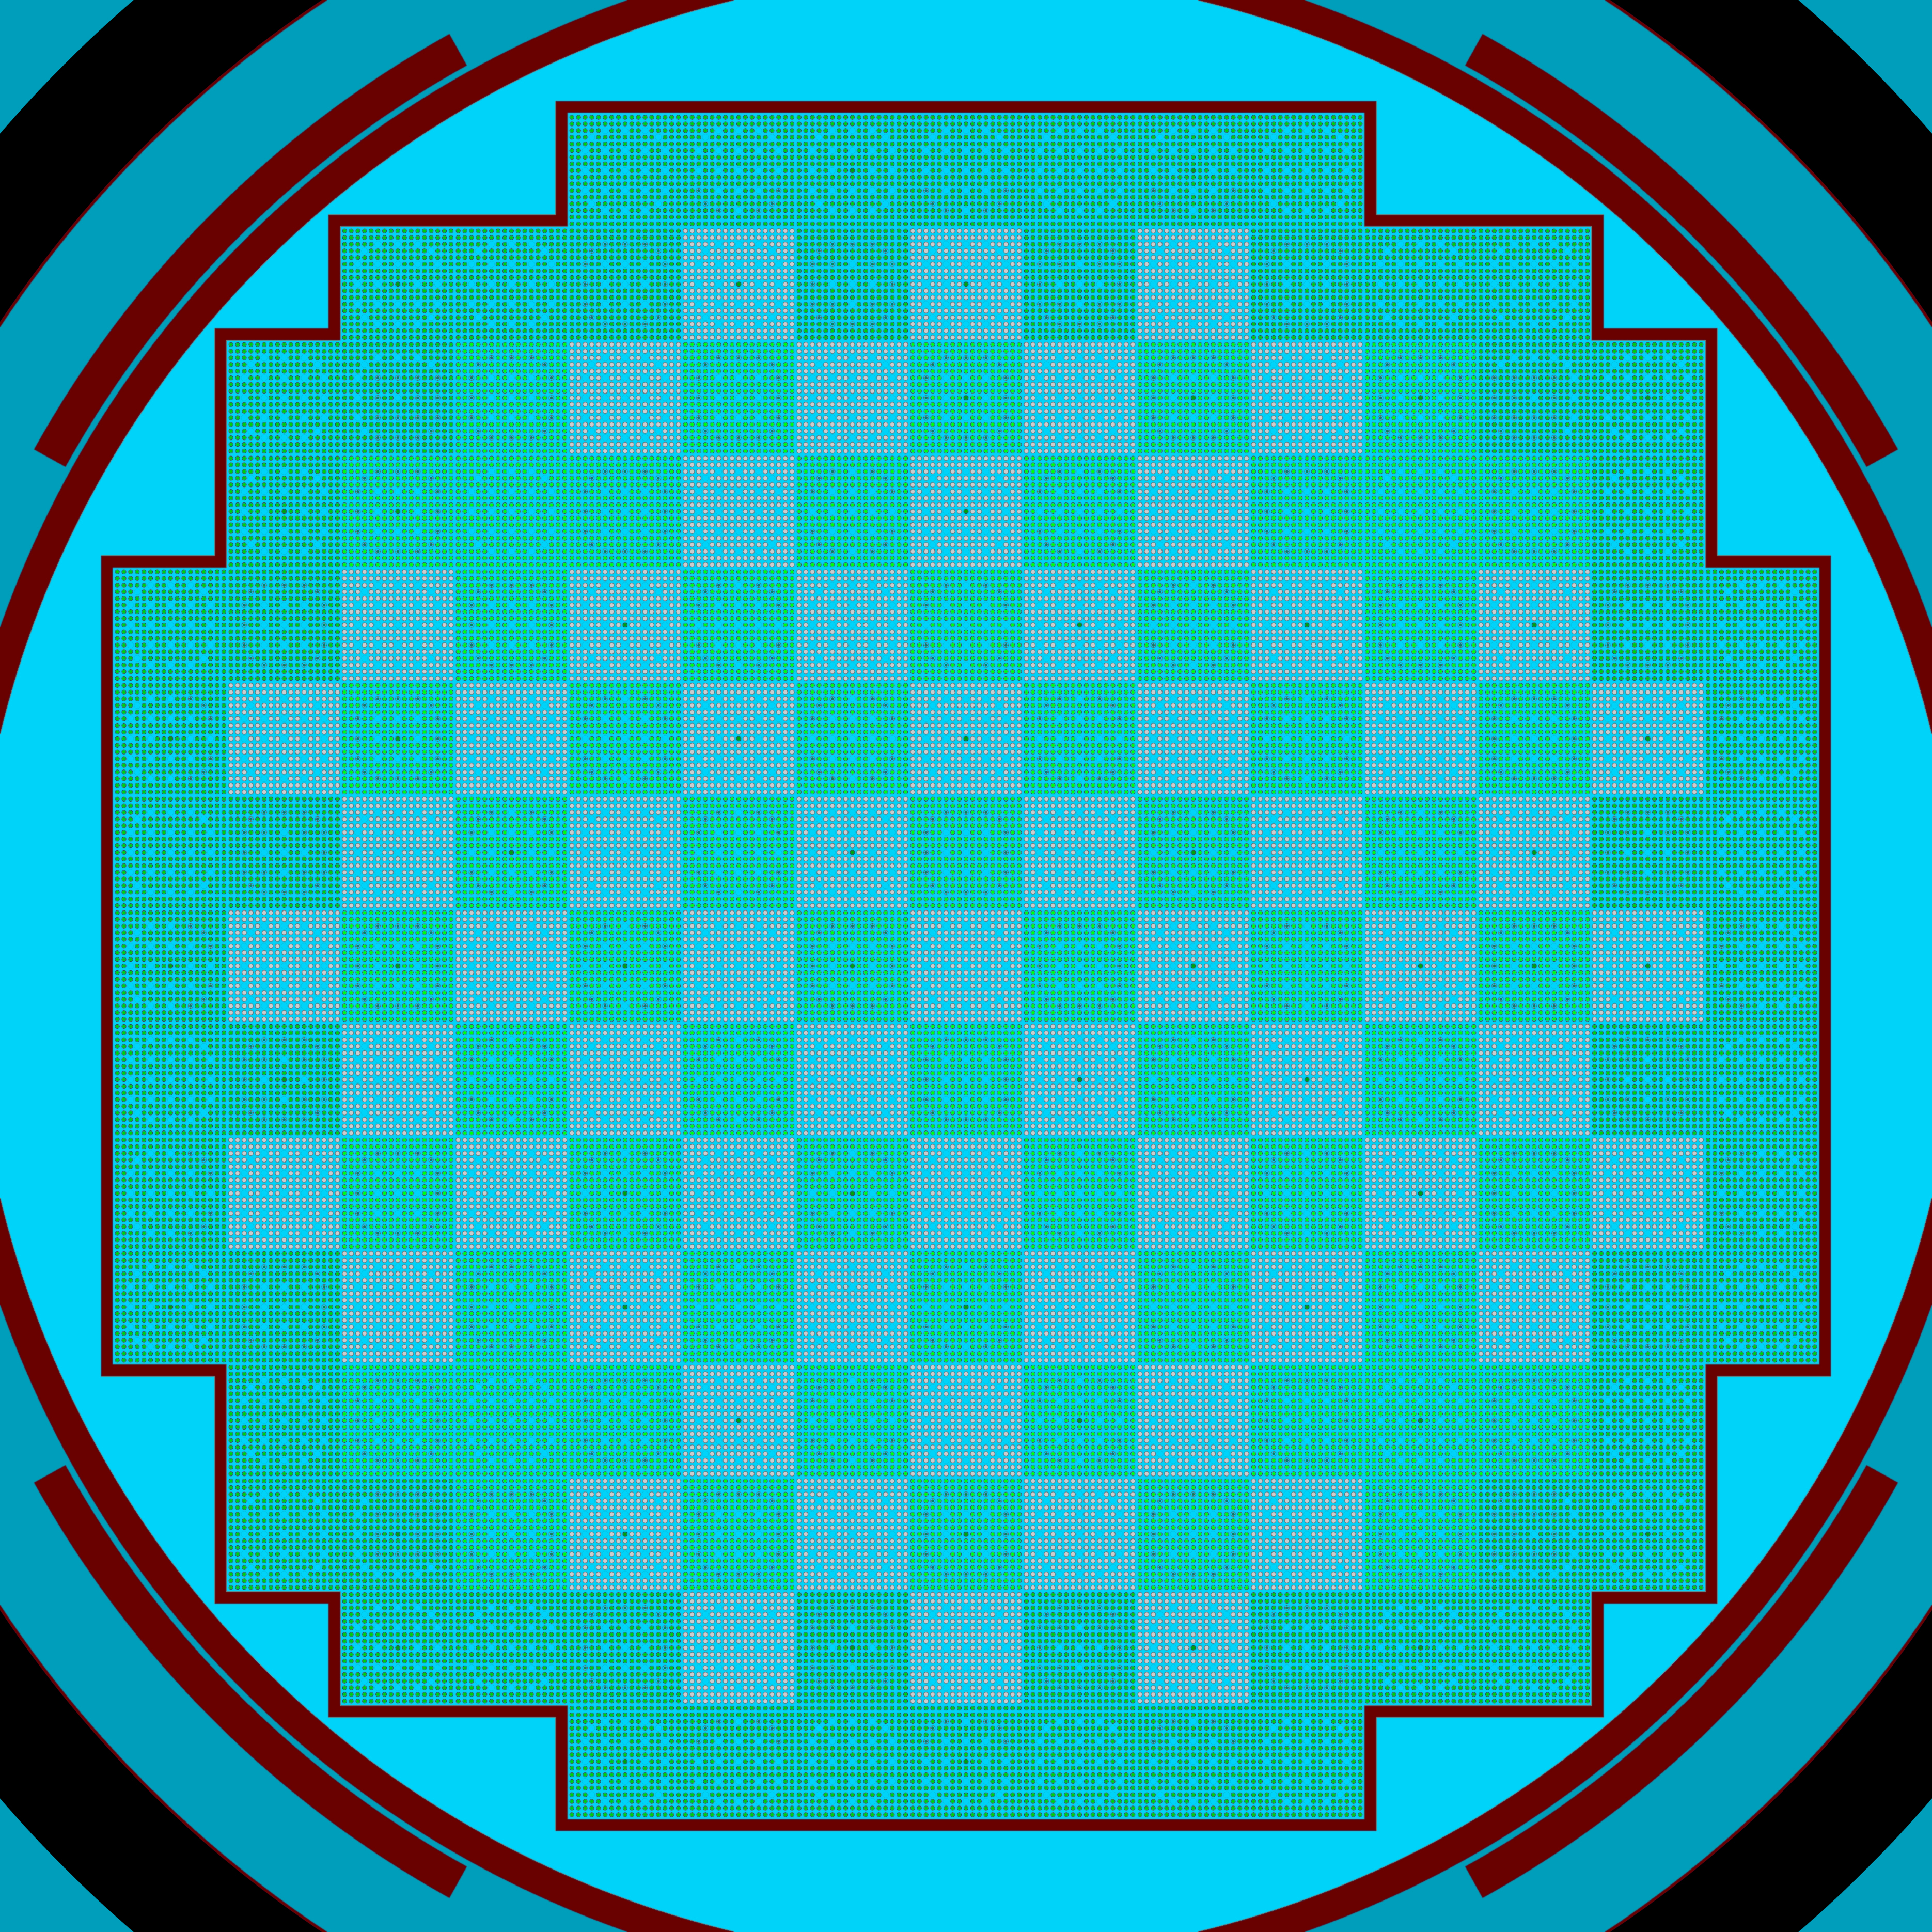
\includegraphics[width=\linewidth]{figures/beavrs-visual/materials-beavrs-radial.jpg}
	\caption{A radial view of the BEAVRS benchmark with regions colored by material.}
	\label{fig:beavrs-materials-radial}
\end{figure} 

\begin{figure}[h!]
	\centering
	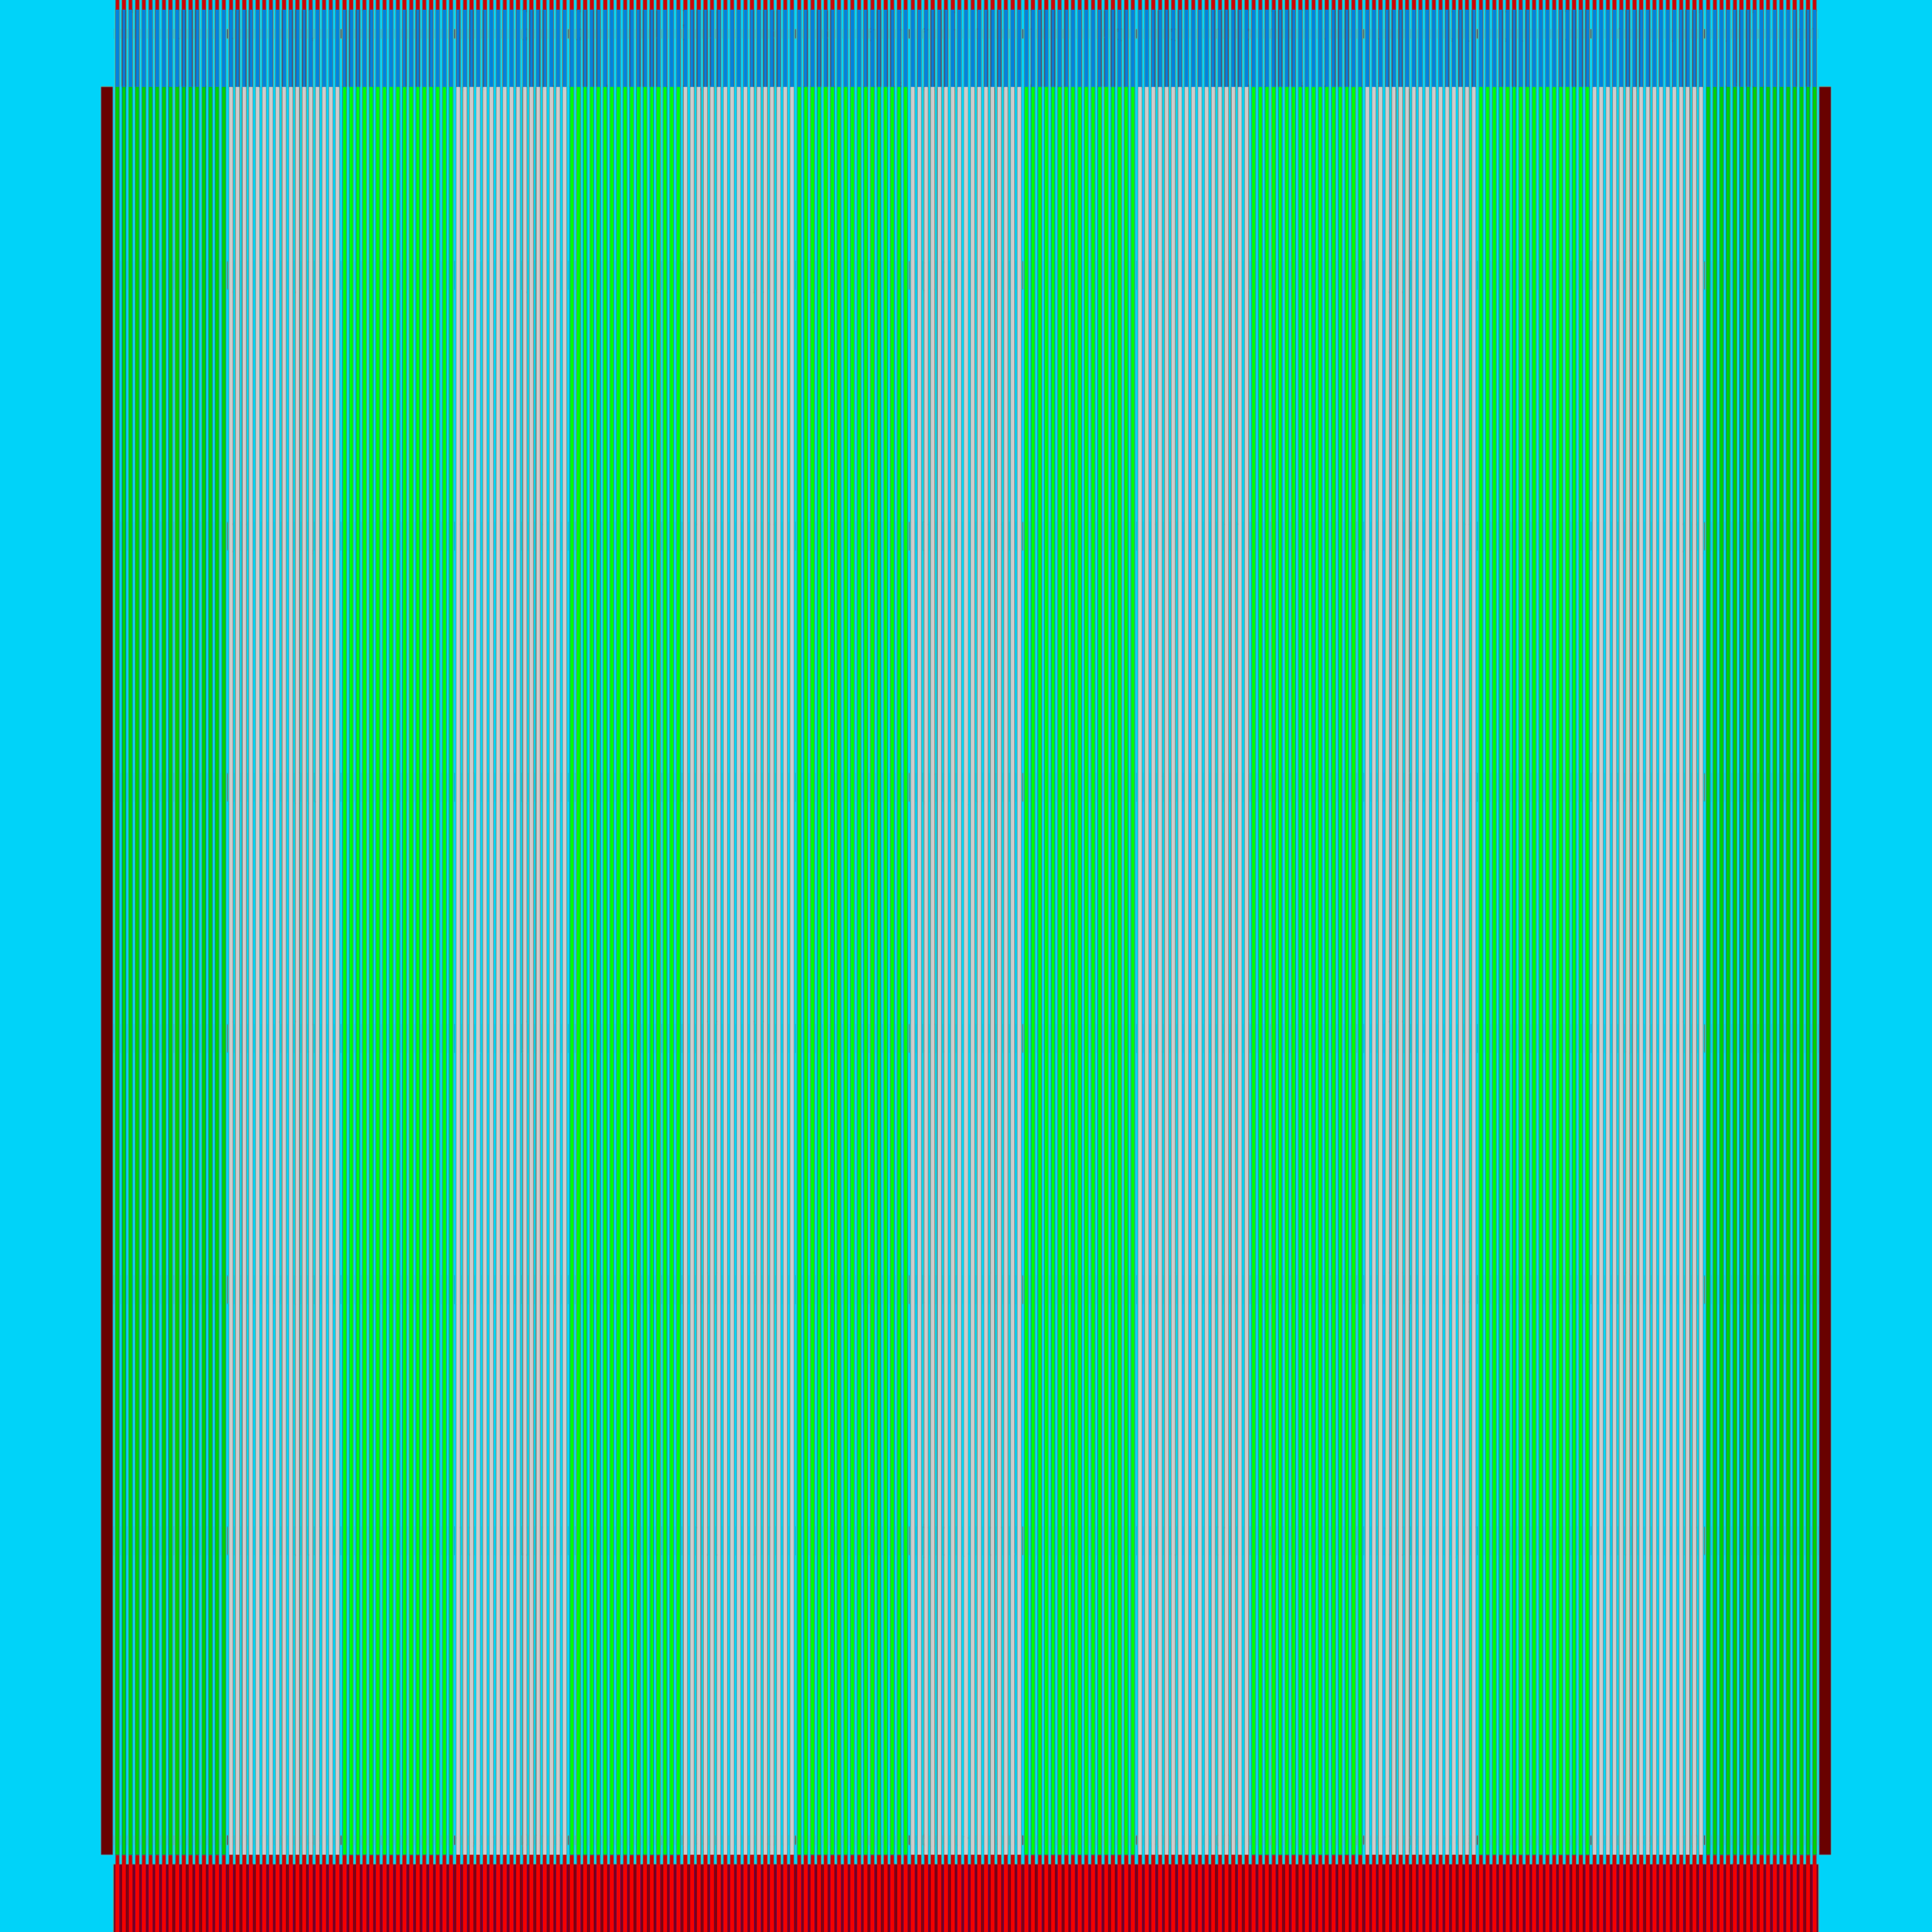
\includegraphics[width=\linewidth]{figures/beavrs-visual/materials-beavrs-axial.jpg}
	\caption{An axial view of the BEAVRS benchmark with regions colored by material.}
	\label{fig:beavrs-materials-axial}
\end{figure} 

\begin{figure}[h!]
	\centering
	\includegraphics[width=0.65\linewidth]{figures/beavrs-visual/materials-single-assembly-radial.png}
	\caption{A radial view of the 1.6\% enriched fuel assembly in the BEAVRS benchmark with regions colored by material.}
	\label{fig:beavrs-single-assembly-materials-radial}
\end{figure} 

\begin{figure}[h!]
	\centering
	\includegraphics[width=0.65\linewidth]{figures/beavrs-visual/materials-single-assembly-axial.png}
	\caption{An axial view of 1.6\% enriched fuel assembly in the BEAVRS benchmark with regions colored by material.}
	\label{fig:beavrs-single-assembly-materials-axial}
\end{figure} 

\newpage
%%%%%%%%%%%%%%%%%%%%%%%%%%%%%%%%%%%%%%%%%%%%%%%%%%%%%%%%%%%%%%%%%%%%%%%%%%%%%%%%
\section{Description of BEAVRS Models}
\label{sec:beavrs-models}

All models which are simulated in this thesis are derived from cutouts of the BEAVRS benchmark with 70 group cross-sections, as described in Appendix~\ref{app:cross-section-gen}. Cutouts are formed in order to evaluate smaller problems which are representative of computational performance or physical behavior of the large full core problem.

\subsection{Full Core 3D Model}
\label{app:beavrs-3D}

The first model is the full core 3D BEAVRS model, incorporating all the details discussed in previous sections. The simulation of this model directly corresponds with the OpenMC simulations from which the cross-sections are derived.


\subsection{Full Core 2D Model}
\label{app:beavrs-2D}

A 2D extruded cutout of the reactor is formed in order to determine the physical behavior of the BEAVRS model in the radial direction. This cutout is taken from a 10 cm axial interval over which there are no grid spacers. Reflective boundary conditions are placed on the top and bottom of the problem. While this model lacks any axial variation, it still contains all radial detail except grid spacers. Due to the lack of axial detail, 2D \ac{MOC} and 3D \ac{MOC} simulations with sufficient parameter refinement should produce equivalent solutions. Only this model and the full core 3D model contain the full radial water reflector. Therefore, this model is very useful in determining the effect of large radial water reflectors. 

\subsection{Single Assembly Model}
\label{app:beavrs-single-assembly}

A single assembly model is formed which represents the full axial detail of a single 1.6\% enriched fuel assembly. While this model lacks radial water reflectors, it contains the full axial detail of the full core problem, including grid spacers. Outside the core, full geometrical detail is also captured including support plate / nozzles and, most notably, water reflectors of approximately 20 cm above and below the fuel. Reflective boundaries are placed on the $x$ and $y$ boundaries. Physically, this is equivalent to an infinite 2D lattice of 1.6\% enriched fuel assemblies. Vacuum boundaries remain on the top and bottom of this model. 

\subsection{Single Assembly Model without Reflectors}
\label{app:trunc-single-assembly}

In addition to the single assembly model, a single assembly model without reflectors is also formed which contains all the detail of the single assembly model, but without the axial water reflectors. Specifically, 20 cm are removed from both the bottom and top of the model, resulting in a model that only covers the active fuel and is 360 cm tall. Axial boundaries conditions are vacuum.

\subsection{SDSA Model}
\label{app:sdsa}

The Single Domain Single Assembly (SDSA) model represents a 20 cm tall cutout within the single assembly model which contains no grid spacers. Reflective boundary conditions are imposed on all surfaces.

\subsection{Short Single Assembly Model}
\label{app:short-single-assembly}

Similar to the SDSA model, the short single assembly model is created which allows for more feasible testing due to its far reduced size. This model is the same as the SDSA model except it is only 10 cm in axial height and contains 3.1\% enriched fuel. This enrichment is the highest enrichment found in the cycle 1 BEAVRS model. The greater fuel enrichment allows for slightly larger gradients with a flux peak in the moderator.


\subsection{Rodded Single Assembly Model}
\label{app:rodded-single-assembly}

The rodded single assembly model is the only model which uses a geometry not explicitly found in the full core 3D BEAVRS model. The model is constructed in the same way as the single assembly model described in Section~\ref{app:beavrs-single-assembly}, but with 3.1\% enriched fuel and with all rods inserted, covering approximately half of the active fuel height. The axial zones of guide tubes containing the inserted control rods are shown in Figure~\ref{fig:control-rod-spec}.

\begin{figure}[htbp]
	\centering
	\begin{tikzpicture}[scale=1,x=1in,y=1in]
	\node[inner sep=0pt,
	text width=3 in,
	minimum size=0.2 in,
	draw=black,
	align=center,
	shift={(0,0.0)}] (n0) {Water};
	\draw[->] (1.7,-0.1) node[right,anchor=west] {0 ~~~~~~~~~~~~~~~~~ Lowest Extent} -- (1.5,-0.1);
	\node[anchor=east] (s0) at (n0.west) {};
	\node[inner sep=0pt,
	text width=3 in,
	minimum size=0.2 in,
	draw=black,
	align=center,
	shift={(0,0.2)}] (n1) {Nozzle / Support Plate Stainless Steel};
	\draw[->] (1.7,0.1) node[right,anchor=west] {20 ~~~~~~~~~~~~~~~ Bottom of Support Plate} -- (1.5,0.1);
	\node[inner sep=0pt,
	text width=3 in,
	minimum size=0.2 in,
	draw=black,
	align=center,
	shift={(0,0.4)}] (n2) {Stainless Steel Pin};
	\draw[->] (1.7,0.3) node[right,anchor=west] {34 ~~~~~~~~~~~~~~~ Bottom of Fuel Rod} -- (1.5,0.3);
	\node[inner sep=0pt,
	text width=3 in,
	minimum size=0.2 in,
	draw=black,
	align=center,
	shift={(0,0.6)}] (n3) {Lower Control Rod Fitting};
	\draw[->] (1.7,0.5) node[right,anchor=west] {240 ~~~~~~~~~~~~~ Botton of Control Rod} -- (1.5,0.5);
	
	\node[inner sep=0pt,
	text width=3 in,
	minimum size=0.2 in,
	draw=black,
	align=center,
	shift={(0,0.8)}] (n4) {Control Rod Lower Absorber Pincell};
	\draw[->] (1.7,0.7) node[right,anchor=west] {242 ~~~~~~~~~~~~~ Bottom of Lower Absorber (AIC)} -- (1.5,0.7);
	\node[inner sep=0pt,
	text width=3 in,
	minimum size=0.2 in,
	draw=black,
	align=center,
	shift={(0,1.0)}] (n5) {Control Rod Upper Absorber Pincell};
	\draw[->] (1.7,0.9) node[right,anchor=west] {344 ~~~~~~~~~~~~~ Bottom of Upper Absorber (B4C)} -- (1.5,0.9);
	
	\draw[->] (1.7,1.1) node[right,anchor=west] {460 ~~~~~~~~~~~~~ Highest Extent} -- (1.5,1.1);
	\draw (1.5,1.3) node[right,anchor=west] {\underline{Elevation (cm)} ~ \underline{Description}};
	
	\end{tikzpicture}
	
	
	\caption[Control Rod Insertion]{Control rod pincell axial specification for the single assembly control rod insertion model.\label{fig:control-rod-spec}}
\end{figure}


The large control rod insertion causes significant gradients within the axial scalar flux distribution, allowing for robust testing of 3D \ac{MOC} on problems with significant axial variation. As mentioned previously, this model uses a separate cross-section library. Instead of simulating the all rods out configuration, which lacks control rods within the core, the rodded single assembly model is explicitly simulated in OpenMC to form cross-section estimates. This allows reasonable estimates of control rod material cross-sections.

%\newpage
%\vfill
%\begin{highlightsbox}[frametitle=Highlights]
%	\begin{itemize}
%		\item The BEAVRS benchmark represents a traditional \ac{PWR} reactor encompassing all relevant radial and axial detail
%		\item The BEAVRS model is simulated within a radially square bounding box, leading to large corner reflector regions
%		\item A 70 group cross-section library is formed through direct simulation of the BEAVRS benchmark in Monte Carlo using the OpenMC \texttt{mgxs} package with a combination of CASMO-4 and in-scatter transport corrections
%		\item Cutouts of the BEAVRS model allow for physics and computational behavior to be tested with much lower computational cost
%		\item A rodded single assembly model is created to test the effect of large axial variation, for which a separate cross-section library is generated in order to accurately capture control rod properties
		
%	\end{itemize}
%\end{highlightsbox}
%\vfill

 % tbr
%\part{Implementation}
% anals
\chapter{Software Design and Development}
\label{chap:software-design}

The work in this thesis uses the OpenMOC~\cite{openmoc} neutron transport code, which was developed for 2D \ac{MOC} simulations, to implement the 3D \ac{MOC} solver. Due to its strict focus on 2D simulations, great work was required to extend OpenMOC to 3D \ac{MOC} calculations. This chapter explains the structure of OpenMOC and the changes that were necessary to increase code flexibility in order to accommodate 3D \ac{MOC} calculations. 

This chapter begins with a general overview of OpenMOC in Section~\ref{sec:openmoc-overview}, with a focus on the Constructive Solid Geometry (CSG) representation of geometric detail. The interested reader can find a more complete description of the OpenMOC code in Boyd's thesis~\cite{boyd2014openmoc}. Next, the object oriented design is discussed in greater detail in Section~\ref{sec:object-oriented} with a focus on the changes to accommodate both 2D and 3D simulations. This discussion is continued in Section~\ref{sec:modular-structure}, where the new modular structure of OpenMOC is discussed as well as its importance in creating a robust simulation tool capable of supporting various algorithms. The computing systems used in this thesis are described in Section~\ref{sec:computing-systems}. Performance considerations are in developing an efficient \ac{MOC} solver are discussed in Section~\ref{sec:software-performance-considerations}. Section~\ref{sec:conv-criteria} discussed the convergence criteria used in this thesis. In Section~\ref{sec:user-input} the standard Python user input is discussed as well as the new C++ alternative build which is attractive for \ac{HPC} applications where the availability of software required for the Python interface may be limited. The chapter is concluded in Section~\ref{sec:version-control} with a discussion of development practices and the open source license.

%%%%%%%%%%%%%%%%%%%%%%%%%%%%%%%%%%%%%%%%%%%%%%%%%%%%%%%%%%%%%%%%%%%%%%%%%%%%%%%%
\section{OpenMOC Overview}
\label{sec:openmoc-overview}

OpenMOC is neutron transport code that is written in C++ with a \ac{SWIG}~\cite{swig} to expose the C++ classes and routines to the Python scripting language. This allows users to take advantage of the simplicity and flexibility of the Python language while also having the performance benefits of C++ compiled code. In this way, users can work entirely in Python without having to touch the underlying C++ code. In addition, users do not have to learn a new input file syntax, only the names, functionality, and input variables of functions constituting the \ac{API}. This allows for users to write more natural code.

The underlying C++ code of OpenMOC also leverages the use of OpenMP~\cite{openmp} for shared memory parallelism. In this framework, all on-node data is shared between threads. With the emergence of the 3D solver, distributed parallelism has also been implemented with MPI~\cite{mpi} in the form of domain decomposition, discussed in Chapter~\ref{chap:domain-decomposition}. With this hybrid parallelism design, OpenMOC is able to scale to both many CPU cores and many nodes. 

OpenMOC is built on the use of \ac{CSG}, which allows complex geometries to be built out of boolean operations -- such as intersections and unions -- of simple surfaces and building blocks termed \textit{primitives}. In addition, a hierarchy is used to agglomerate collections of primitives together. This approach is particularly useful for reactor geometries which are often highly structured. For example, a typical reactor core is built out of simple \textit{fuel pins}, grouped together into \textit{assemblies}. Fuel pins describe the radial detail of a fuel rod. Assemblies are then grouped together to form the reactor core. An example of a 2D \ac{CSG} construction of a single assembly is given in Figure~\ref{fig:core-csg}.

\begin{figure}[h!]
	\centering
	\includegraphics[width=0.9\linewidth]{figures/assembly-csg.PNG}
	\caption[]{The hierarchical CSG construction of a typical assembly.}
	\label{fig:core-csg}
\end{figure}

One of the benefits of the \ac{CSG} approach is a reduced memory requirements of storing the geometry. Instead of explicitly storing the geometry information of each fuel pin within the reactor core, only unique fuel pin types need to be stored. They are then referenced by their parent structure. For instance, an assembly containing a lattice of fuel pins creates a mapping of lattice location to the unique fuel pin type, rather than replicating the full geometric information for each fuel pin.

In addition, the formation of a \ac{CSG} allows ray tracing to be conducted in a general framework, agnostic of the individual primitives. Each \textit{cell} in OpenMOC is defined in terms of of \textit{surface} objects and the half-space of each surface. A half-space determines on which side of the surface the cell is located. Ray tracing fundamentally involves calculating the distance to intersection along a direction. With the \ac{CSG} framework, each of the bounding surfaces is queried for the distance to intersection. This naturally speeds up ray tracing by not having to check each instance of a surface within the geometry, but rather only the local surfaces. 

Once the geometry is built, OpenMOC generates tracks across the constructed geometry, and solves the neutron transport equation iteratively, as described in Chapter~\ref{chap:moc}. CMFD acceleration can also be included by the user, which utilizes the methods described in Chapter~\ref{chap:cmfd}.

Once the neutron transport equation is solved, the solver can be queried to return the scalar flux distribution as well as reaction rates. In order to visualize the data, OpenMOC includes Python plotting routines for scalar flux data, computed reaction rates, as well as geometric detail and visual diagnostics. 


%%%%%%%%%%%%%%%%%%%%%%%%%%%%%%%%%%%%%%%%%%%%%%%%%%%%%%%%%%%%%%%%%%%%%%%%%%%%%%%%
\section{Object Oriented Design}
\label{sec:object-oriented}

OpenMOC uses the object oriented programming paradigm whereby data structures called \textit{classes} are created that encapsulate both the data and associated subroutines. Object oriented programming generally leads to more resilient code since only the class itself can access its private attributes. An instantiation of a class is termed an \textit{object}. OpenMOC applies many of the principles of object oriented programming including information hiding, inheritance, and polymorphism.

An OpenMOC simulation requires three main components: a geometry, a track generator, and a solver. All of these are C++ classes in OpenMOC and exposed to the user. The user first describes the surfaces, cells, universes, and materials which constitute the geometry in a hierarchical \ac{CSG} arrangement. The user then instantiates a \texttt{Geometry} object and provides it the root cell of the \ac{CSG}. Next, a \texttt{TrackGenerator} is instantiated which is provided the \texttt{Geometry} object as well as track generation parameters such as radial ray spacing and number of azimuthal angles. Lastly, a \texttt{Solver} object is instantiated and provided the \texttt{TrackGenerator} object along with solver criteria such as the tolerance. The solver can then be called to solve the \ac{MOC} equations, such as the \ac{MOC} neutron transport eigenvalue problem, using the track and segmentation information found in the \texttt{TrackGenerator}.

Extending the OpenMOC solver to 3D simulations required restructuring all of these classes in order to make them more flexible. A focus in extending the sovler to 3D simulations was to still maintain the ability to run 2D simulations. A benefit of maintaining the ability to run 2D simulations is to allow the user to compare 2D and 3D simulations on the same problem. To accommodate this, the input structure between 2D and 3D simulations is very similar. In order to make the code more resilient and simpler, common code reuse was emphasized. Many of the routines present in the 2D simulations are also used in the 3D simulations so both should use the same code without re-writing those entire sections. These points illustrate the need for maximum cohesion between the 2D and 3D solver modes. This is accomplished by expanding the 2D classes to be more general.

\subsection{\texttt{Geometry} Class Updates}
\label{sec:oo-geometry}

The \texttt{Geometry} class was altered to accommodate piecewise \textit{axially extruded geometries}. Axially extruded geometries are geometric configurations in which the geometry looks the same at every axial level. A piecewise axially extruded geometry is a geometry that can be formed as the union of a finite number of extruded geometries. For instance, a fuel rod with end caps would fit the description of a piecewise axially extruded geometry but a sphere would not. Most practical reactor applications are indeed piecewise extruded geometries so this is not a very strong limitation. 

With the change from 2D geometries to piecewise axially extruded geometries, circles are transformed to $z$-cylinders (cylinders with a vertical major axis) and $z$-planes are added with a similar structure to the $x$ and $y$ planes already incorporated in OpenMOC. With this new geometry paradigm, 2D problems are thought of as simulating a radial slice of a 3D geometry at a given $z$ height. 

\subsection{\texttt{TrackGenerator} Class Updates}
\label{sec:oo-trackgenerator}

The \texttt{TrackGenerator} class was updated to generate tracks and ray trace, compatible with the updated \texttt{Geometry} class. 2D ray tracing is imagined as ray tracing tracing perpendicular to the $z$-axis at some $z$-height. By default this height is assumed to be 0.0 in order to limit the complexity of user input for 2D simulations. The user can specify a different $z$-height using the \texttt{setZCoord} function of the \texttt{TrackGenerator} class.

For 3D simulations, a new \texttt{TrackGenerator3D} class was created which inherits from the \texttt{TrackGenerator} class. In object oriented programming, a class that inherits from a parent class has access to all the parent class data and subroutines. Since tracks are built on a 2D projection, the 3D track generator must have all the functionality of the regular 2D track generator. This is the typical paradigm where class inheritance is useful. 

During ray tracing, a \texttt{TrackGenerator3D} object first ray traces all 2D tracks (determined from the parent \texttt{TrackGenerator} functionality) over all potentially unique $z$-planes in the geometry to form the equivalent of a ray trace over the composite of all radial detail in the geometry. Since this can potentially be expensive, users are allowed to indicate the unique piecewise axially extruded ranges in the \texttt{Geometry} through the \texttt{setSegmentationZones} function in the \texttt{TrackGenerator3D} class. If these zones are not specified, all $z$-planes in the geometry are viewed as a potential divider between different axially extruded regions.

Once the 2D ray trace is conducted over all axially extruded regions, the full 3D ray trace can be calculated. Due to the expense of explicitly storing all 3D tracks in a typical geometry, the \texttt{TrackGenerator3D} class generates tracks on-the-fly. Similarly, segments can be prohibitively expensive to store. Therefore, the default mode is to calculate segments on-the-fly rather than upfront, although both options are available. Ray tracing and segmentation is discussed in greater detail in Chapter~\ref{chap:ray-tracing}.

\subsection{\texttt{Solver} Class Updates}
\label{sec:oo-solver}

The \texttt{Solver} class has also been reformulated to support both 2D and 3D simulations. The \texttt{Solver} class is an abstract class, meaning it contains the description of data and associated subroutines, but cannot be instantiated on its own. Instead, there are subclasses that inherit from the abstract class that can be instantiated. In this case the \texttt{CPUSolver} and \texttt{GPUSolver} classes are both subclasses of the \texttt{Solver} class. Rather than supporting both the \texttt{CPUSolver} and \texttt{GPUSolver} classes, this thesis focuses on the \texttt{CPUSolver} class to allow for easier implementation of the object oriented structures.

The \texttt{CPUSolver} was altered to support the calculation of both 2D \ac{MOC} and 3D \ac{MOC} equations. By referring to the supplied \texttt{TrackGenerator} object, it can determine whether a 2D or 3D simulation should be calculated. If a \texttt{TrackGenerator3D} object was provided to the solver, it runs a 3D simulation. Otherwise, a 2D simulation is run. While much of the code is shared between the 2D and 3D simulations in the solver, the core code which calculates the variation of angular flux over segments has separate 2D \ac{MOC} and 3D \ac{MOC} code sections in order to maximize performance.

In addition to the existing \texttt{CPUSolver}, a new \texttt{CPULSSolver} class has been added to OpenMOC which is capable of using a linear source approximation. Since the linear source solver needs much of the code present in the regular flat source solver, \texttt{CPULSSolver} was implemented as a subclass of \texttt{CPUSolver}.

%%%%%%%%%%%%%%%%%%%%%%%%%%%%%%%%%%%%%%%%%%%%%%%%%%%%%%%%%%%%%%%%%%%%%%%%%%%%%%%%
\section{Modular Structure}
\label{sec:modular-structure}

In altering OpenMOC to support both 2D and 3D simulations, it was quickly realized that without a massive overhaul, there would be a very large amount of repeated code. The goal was to create code that was capable of conducting both 2D and 3D \ac{MOC} simulations, but also compare multiple types of ray tracing and mathematical approximations (such as linear source). For all these options to be supported, there is the possibility for much of the same functionality to be implemented at multiple points in the code.

For example, \ac{MOC} can largely be described as an algorithm that performs a ray trace and then computes equations over the segments formed from the ray trace. Many different ray tracing algorithms could be used with the underlying equations and solver remaining theoretically unchanged. However, if the code is rigid, each new ray tracing algorithm would require an entire code re-write.

Therefore, a goal in developing OpenMOC to support work presented in this thesis is to maximize code reuse. This not only shortens the code but also makes it more robust as algorithms tend to change frequently to update functionality and fix bugs. If code is repeated, it is likely that not all of the code would receive the appropriate updates. Additionally, comparing options in the code, such as ray tracing, becomes much more robust when the code run during comparisons only differs minimally with most of the differences being those directly tested.

A structure was created in which segment traversal, ray tracing, and the algorithms that use segment information could be easily decoupled. In this new structure, \texttt{MOCKernel} classes dictate what operations to perform on each segment and a \texttt{TraverseSegments} class dictates how to iterate over segments and which ray tracing method to use. Both of these classes are virtual classes which have subclass implementations. Specific algorithms that use segment information are formed as subclasses of the \texttt{TraverseSegments} class, each defining operations to perform on groups of segments. The algorithms should also specify which \texttt{MOCKernel} objects to use.

\subsection{\texttt{MOCKernel} Classes}

Since the \texttt{MOCKernel} class operates directly on segments, it appears in the inner-most loop in algorithms. The \texttt{MOCKernel} parent class contains common information used for most of its subclass implementations. These attributes include:
\begin{itemize}
	\item A counter for the number of segments encountered by the kernel
	\item The maximum path length allowed for segments before they must be split
	\item The number of energy groups
\end{itemize}

An \texttt{MOCKernel} class also has a few virtual functions that must be implemented by subclasses. Notable functions include:
\begin{itemize}
	\item An \texttt{execute} function which dictates what to do on a segment
	\item A \texttt{newTrack} function that dictates functionality when a new group of segments is encountered.
\end{itemize}
The \texttt{execute} function is applied immediately when a segment is formed from ray tracing (or loaded in the case of explicitly stored segments) whereas the \texttt{newTrack} function is applied at the start of sequencing through a group of segments. The segments comprising a track is an example of a common grouping of segments, though other groupings could be chosen.

Since the \texttt{MOCKernel} class is a virtual class, it is meant to have subclasses which can be instantiated. The current \texttt{MOCKernel} subclasses implemented in OpenMOC are:
\begin{itemize}
	\item \texttt{CounterKernel}: Counts the number of segments encountered by the kernel
	\item \texttt{VolumeKernel}: Uses track weights and segment lengths to form an estimate of the volumes of regions encountered
	\item \texttt{TransportKernel}: Directly applies the transport equation on the encountered segments
	\item \texttt{SegmentationKernel}: Caches segment information for use in later calculations
\end{itemize}
Since the \texttt{SegmentationKernel} object just caches information it is useful for complicated operations or operations which can be most efficient when applied to a bulk grouping of data. For this efficiency reason, the \texttt{TransportKernel} is not currently used in the default solver. Instead, a \texttt{SegmentationKernel} is used in its place so that the operations can be applied to flux data at once instead of interleaving ray tracing with transport calculations.

\subsection{\texttt{TraverseSegments} Classes}

Unlike the \texttt{MOCKernel} parent class, the \texttt{TraverseSegments} virtual class contains a significant amount of algorithmic information. Specifically, the virtual class contains all segment iteration and ray tracing algorithms. The algorithm has a \texttt{loopOverTracks} function that takes an \texttt{MOCKernel} as an argument. Subclasses of \texttt{TraverseSegments} can call this function which iterates over groups of segments (eg. tracks). 

Inside the \texttt{loopOverTracks} function, a conditional block calls the appropriate segment looping scheme, passing along the provided kernel. The currently implemented segment iteration schemes are:
\begin{itemize}
	\item \texttt{loopOverTracks2D}: Iteration scheme for looping over explicitly stored 2D segments
	\item \texttt{loopOverTracks3DExplicit}: Iteration scheme for looping over explicitly stored 3D segments
	\item \texttt{loopOverTracksByTrackOTF}: Iteration scheme for looping over and generating segments on-the-fly where segments in a track are looped over in order before switching to the next track
	\item \texttt{loopOverTracksByStackOTF}: Iteration scheme for looping over and generating segments on-the-fly where segments in a $z$-stack of tracks are looped over in order before switching to the next $z$-stack
\end{itemize}
Each of the iteration schemes loops over all tracks and segments in the problem in some order, performing the associated ray tracing algorithm when appropriate. The ray tracing scheme is provided information relevant to ray tracing or loading the segments of interest. In most cases, this pertains to all segments in a track. However, for the \texttt{loopOverTracksByStackOTF} scheme, all segments in a $z$-stack are traced at once. Before calling the ray tracing scheme, the \texttt{newTrack} function of the provided kernel is called. Then the ray tracing scheme is called and provided the kernel so that it can call the \texttt{execute} function immediately when the segment is formed or loaded. 

After the ray tracing scheme is completed, an \texttt{onTrack} function is called which details operations to perform on the group of segments. The cached segment information is also provided if a \texttt{SegmentationKernel} was used. The transport sweep algorithm currently used in OpenMOC applies all of the \ac{MOC} equations inside the \texttt{onTrack} function using the provided cached segment information.

In general, algorithms which require track or segment information should form a small subclass of the \texttt{TraverseSegments} function and define the \texttt{onTrack} function. Additionally, an \texttt{execute} function should be defined which details the general structure of the algorithm. It should include the setup, call the \texttt{loopOverTracks} function to loop over all segments and apply the algorithm defined by the \texttt{onTrack} function and the provided kernel, and then detail any operations to perform after looping over all tracks and segments. 

An example of an execute function is given below for the \texttt{VolumeCalculator} class which calculates the volumes of all regions in the geometry. Since it performs all operations directly on segments using \texttt{VolumeKernel} objects, the \texttt{onTrack} function is defined to simply return.

\begin{center}
\begin{lstlisting}
void VolumeCalculator::execute() {
	#pragma omp parallel
	{
		MOCKernel* kernel = getKernel<VolumeKernel>();
		loopOverTracks(kernel);
	}
}
\end{lstlisting}
\end{center}

For algorithms in which only operations need to be performed on tracks, a \texttt{NULL} kernel can be provided which alerts the segment iteration scheme to skip the ray tracing step. Numerous subclasses of \texttt{TraverseSegments} are present in OpenMOC since every algorithm which loops over segments or tracks is contained in a subclass of \texttt{TraverseSegments}. They all appear in the files \texttt{TrackTraversingAlgorithms.h} and \texttt{TrackTraversingAlgorithms.cpp}.

%%%%%%%%%%%%%%%%%%%%%%%%%%%%%%%%%%%%%%%%%%%%%%%%%%%%%%%%%%%%%%%%%%%%%%%%%%%%%%%%%
\section{Computing Systems}
\label{sec:computing-systems}

In this thesis, all computational results either use the Argonne BlueGene/Q supercomputer or the Falcon supercomputer at the Idaho National Laboratory. An overview of system parameters is shown in Table~\ref{tab:system-params}. Note that the BlueGene/Q architecture uses significantly slower cores. In addition, these cores have limited branch prediction capabilities, causing them to be much slower. The Argonne BlueGene/Q supercomputer contains two partitions of interest in this thesis: the Cetus partition and the Mira partition. The Cetus partition is intended for small simulations whereas the Mira partition is intended for large simulations.

\begin{table}[ht]
	\centering
	\caption{Description of single node supercomputer architectures}
	\medskip
	\begin{tabular}{c|c|c}
		\hline
		& Argonne BlueGene/Q & Falcon\\
		\hline
		CPU Type & Single Socket & Dual Socket \\
		CPU Name & BlueGene/Q & E5-2695 v4 \\
		Architecture & PowerPC A2 & Broadwell\\
		Cores per Node & 16 & 36\\
		Hardware Threads per Node & 64 & 36\\
		Speed (GHz) & 1.6 & 2.1\\
		Node Memory (GB) & 16 & 128 \\
		\hline
	\end{tabular}
	\label{tab:system-params}
\end{table}

%%%%%%%%%%%%%%%%%%%%%%%%%%%%%%%%%%%%%%%%%%%%%%%%%%%%%%%%%%%%%%%%%%%%%%%%%%%%%%%%
\section{Performance Considerations}
\label{sec:software-performance-considerations}

So far this chapter has emphasized software design for code resiliency and flexibility. However, a useful application should also minimize runtime. This section concentrates on software design considerations to maximize performance and minimize runtime.

\subsection{Addressing Performance in Object-Oriented Modular Software Design}

While the object-oriented and modular design is useful for code reuse, minimizing the number of potential bugs and allowing for greater flexibility, it does add some computational overhead. The overhead is largely due to added function calls. This can be overcome through the use of \textit{inline functions} which inject their code directly into sections where they are called at compile time. While this increases the performance of the code, it can radically increase the size of the executable, especially for large inline functions. Therefore, functions should only be inline functions if they are small. For instance, inline functions are used in OpenMOC for computing surface intersections and tallying current to CMFD surfaces. 

However, successfully using inline functions can sometimes be difficult where logic is required to determine which function to call. Therefore, performance-sensitive code should be designed such that the number of function calls which are not inline functions are minimized.

The optimal code design blends object oriented and modular design for code that is not performance-critical while using optimized and less flexible code for the performance-sensitive sections. In terms of the \ac{MOC} algorithm, over 95\% of the runtime is typically spent applying the \ac{MOC} equations for a given segment. In OpenMOC, the application of the \ac{MOC} equations occurs in the \texttt{CPUSolver::tallyScalarFlux} function. This function, which is quite small in size, should be thoroughly optimized for performance while the rest of the code should rely heavily on object oriented and modular design principles. 

\subsection{Organizing Data Contiguously in Energy Groups}

One critical consideration when designing performance-sensitive code is the memory layout. When CPU cores load information from memory, they load entire cache lines into local caches rather than just the desired variable. This allows the number of loads to be reduced if nearby memory is accessed. When desired memory is already within cache, it is termed a \textit{cache hit}. If it is not, it is termed a \textit{cache miss}, requiring an extra load. Optimizing cache performance to maximize cache hits is critical when designing efficient software, as loads from main memory can be quite expensive. \textit{Locality} refers to how well memory is organized such that nearby or local memory is accessed frequently. 

To maximize locality in \ac{MOC} applications, the data should be structured to be contiguous in energy groups. Generally, the \ac{MOC} equations can be approached as being applied to segments over several energy groups. Since \ac{MOC} tracks traverse regions in different orderings, it is difficult to optimize the cache efficiency of data accessed by region. However, the data for each region can easily be structured and always traversed in the same ordering. Therefore, the maximal amount of work should be completed on each region before moving to the next. This implies that the energy groups should all be treated together and the data structures should be contiguous in energy groups to reflect this memory access pattern. 

\subsection{Scratch Pads for Temporary Storage}

There are several points throughout the \ac{MOC} algorithm where quantities need to be temporarily stored by region or by group. One example is calculating total reaction rates. To compute a total reaction rate in the reactor, the reaction rates from all regions and energy groups need to be calculated and summed. It is possible to add each contribution from a region and group to a tally for the total reaction rate immediately after calculation, but this can lead to significant roundoff error. Alternatively, if the summed values could be first stored in an array and then added in a pairwise fashion, the roundoff error can be significantly reduced~\cite{pairwise}.

The number of summed quantities is $NG$ where $N$ is the number of source regions and $G$ is the number of energy groups. An array of $NG$ could be allocated, but this would require a significant amount of additional storage. Instead, two arrays are allocated -- one of size $G$ and another of size $N$. Reaction rates for all $G$ groups for an individual region are computed and then stored in a temporary array of size $G$. This array is then summed using a pairwise sum. The result is then stored in an array of size $N$. After this conducted for all $N$ regions, the array of size $N$ is then summed in a pairwise fashion.

Since temporary arrays of size $N$ and size $G$ are often found throughout OpenMOC, memory for these arrays is allocated at the beginning of the solver for each thread. Allocating memory can often be quite costly. If the arrays were allocated just before use, there would be a significant number of memory allocations. By allocating the memory up front and later referencing the allocated memory, the number of memory allocations is minimized, improving performance.

\subsection{Minimizing Parallel Contention}

When multiple threads modify shared data, bugs can be incurred due to race conditions where the outcome of a program is dependent on the order in which threads execute operations. For instance, consider multiple threads adding numbers to a shared counter. The fundamental operations that access the data are reads and writes. Therefore, one thread could read a value of the counter and before the thread adds the read value with its added value, the counter updates. The thread then writes the computed value to the shared counter, disregarding the update that occurred after the read, leading to an error in the computation. This occurs because the read, addition, and write are separate operations where the data can be modified between the operations~\cite{shavit}.

Because of these considerations, care must be taken to ensure correctness in multi-threaded applications. A common way to ensure correctness is to place a \textit{lock} around \textit{critical sections}. A critical section is where shared data is potentially modified by multiple threads. A lock ensures that at most one thread can access the critical section at any time. While locks do ensure correctness, they can also cause a bottleneck in the code, especially when many threads are present and attempting to access the same critical section. This situation is termed \textit{contention}.

In terms of the \ac{MOC} algorithm, in which each thread is responsible for applying the \ac{MOC} equations to a group of segments, threads can be handling segments which access and modify data (such as the scalar flux) for the same region. A naive implementation would place a lock around the modification of the local scalar flux data for each energy group when the segment's contribution is computed. While this ensures correctness, it requires that each thread attempt to acquire a lock for each energy group, which can incur significant overhead cost.

Instead, each thread tallies the contributions to each energy group in its local temporary storage array, as mentioned in the previous section. This allows for the thread to modify the array without any contention with other threads. After the contributions are computed and stored for every energy group, a lock is acquired for the region and the local thread contributions are summed to the global tally of scalar flux. This allows for only one lock to be acquired for each segment traversal. In addition, it allows for increased cache efficiency and vectorization. Lock operations require communication between cache levels to ensure correctness and are not vectorizable. By decreasing the frequency to which locks are accessed, these issues can be minimized. This was thoroughly tested during the development of a prototype application named SimpleMOC~\ref{simplemoc}.

\subsection{Computing Exponentials}

One major bottleneck of \ac{MOC} solvers, particularly for flat source \ac{MOC}, is the computation of exponentials. Since an exponential term is present in the \ac{MOC} equations, dependent on optical path length, an exponential needs to be computed for each segment and group. Specifically, $1-e^{-\tau}$ needs to be computed, where $\tau$ is the optical path length. 

A naive approach would just use the intrinsic \texttt{exp} function available in the standard C++ library. While this would accurately compute the exponential, the intrinsic \texttt{exp} function can be quite expensive. Boyd showed that for the initial flat source implementation of OpenMOC, it was far more efficient to compute exponentials with a table lookup~\cite{boyd2014openmoc}. This is accomplished by first allocating a table of exponential values (specifically $1-e^{-\tau}$) as a function of optical path length $\tau$. This table only ranges from optical path lengths up to the maximum optical path length in the problem to reduce table size, allowing for it to more easily fit in cache. Boyd implemented the table lookup using linear interpolation, but the work in this thesis implements a quadratic lookup table, allowing for the table size to be reduced even more.

The computation of the exponential will be further addressed in Chapter~\ref{chap:linear-source} where the linear source implementation is addressed. In addition to discussing the implications of exponential computation for linear source, optimized exponential functions will also be discussed.

\subsection{Floating Point Precision}

Another performance consideration is the precision to use for floating point variables -- either single or double precision. In general, all accumulators, which store the summation of many terms, are stored in double precision because they are sensitive to roundoff error. Common examples include the eigenvalue $k$ and residual estimates. On the other hand, values which are less likely to have an impact on results due to roundoff error are stored in single precision.  For instance, the angular fluxes are always stored in single precision. This allows for the memory footprint to be reduced and cache efficiency to be maximized as twice as much data can be stored in cache.

Some variables allow for either single or double precision, depending on specified compiler options. Specifically, the types \texttt{FP_PRECISION}, \texttt{SF_PRECISION}, and \texttt{CMFD_PRECISION} are all defined to be either single or double precision floating point types at compile time. The \texttt{FP_PRECISION} type dictates the precision of the majority of toggled data, including the exponential table and cross-section data.  The \texttt{SF_PRECISION} type dictates the precision of scalar flux data and the \texttt{CMFD_PRECISION} dictates the precision of CMFD matrices and linear algebra solvers.

The \texttt{SF_PRECISION} type, dictating the precision of scalar flux data is defined separate from \texttt{FP_PRECISION} to independently treat the way scalar flux tallies are handled. On one hand, scalar flux data can be viewed as accumulators since many segments tally their contribution to the scalar flux in each region. However, the data footprint of scalar flux data can also be significant and impact the performance of the solver.

For high performance computing problems, all the precision types are typically set to single precision in order to maximize performance. However, when very tight convergence is desired, normally for debugging purposes, all precision types are set to double precision. In this thesis, all timing results presented use single precision, but double precision is used for cases where convergence behavior is analyzed to tight convergence.

To test the effect of floating point precision, simulations of the SDSA test problem introduced in Section~\ref{sec:sdsa} are conducted with the modular track laydown which will be introduced in Chapter~\ref{chap:track-laydown}, on-the-fly ray tracing by $z$-stack introduced in Chapter~\ref{chap:ray-tracing}, and the linear source solver introduced in Chapter~\ref{chap:linear-source}. The aim is to show performance differences from using single or double precision. Here, only one transport sweep iteration is conducted without \ac{CMFD} acceleration. The \ac{MOC} parameters used in the tests are those presented later in Table~\ref{tab:final-params} and the results are presented in Table~\ref{tab:precision-results}. In these tests, the reported precision refers to the precision of both \texttt{SF_PRECISION} and \texttt{FP_PRECISION}. The tests were conducted using all 36 cores on one node of the Falcon supercomputer. For each precision, three simulations were conducted with the runtime uncertainty reported as the maximum difference from the mean of the three tests.

\begin{table}[ht]
	\centering
	\caption{Effect of floating point precision on performance of the SDSA test problem}
	\medskip
	\begin{tabular}{lcc}
		\hline
		 & Single Precision & Double Precision \\
		 \hline
		Total Memory (GB) & 12.49 & 12.81 \\
		Boundary Angular Flux Storage (GB) & 12.15 & 12.15 \\
		Scalar Flux Storage (GB) & 0.39 & 0.76\\
		Scalar Flux Moments Storage (GB) & 0.78 & 1.52 \\
		Runtime (sec) & 98 +/- 7 & 100 +/- 6 \\
		\hline
	\end{tabular}
	\label{tab:precision-results}
\end{table}

Note that boundary angular fluxes are always stored in single precision. The single precision boundary angular flux storage accounts for 94.8\% of total memory when the \texttt{SF_PRECISION} and \texttt{FP_PRECISION} types set to double precision. When these types are set to single precision, boundary angular flux storage accounts for 97.3\% of total memory. Since boundary angular flux storage accounts for the vast majority of memory consumption, the memory footprint of OpenMOC would almost directly double if the boundary angular fluxes were stored in double precision.

The effect of single or double precision for the \texttt{SF_PRECISION} and \texttt{FP_PRECISION} types on runtime is not obvious, as the difference is less than the reported uncertainties. The total memory footprint is only slightly reduced by using single precision. The effect of \ac{CMFD} precision on runtime is not tested in these studies, but the final results presented in this thesis will show the computational cost of the \ac{CMFD} solver to be insignificant for the targeted full core simulations with \ac{MOC} parameters chosen to sufficiently converge the solution is space and angle.

%%%%%%%%%%%%%%%%%%%%%%%%%%%%%%%%%%%%%%%%%%%%%%%%%%%%%%%%%%%%%%%%%%%%%%%%%%%%%%%%
\section{Convergence Criteria}
\label{sec:conv-criteria}

Since the \ac{MOC} equations are converged iteratively with source iteration, a convergence tolerance must be chosen for the simulation. In this thesis, convergence is determined by iterative change in the neutron production rate. Specifically, the neutron production rate $f_i$ in a source region $i$ can be computed with a sum of contributions from all $G$ energy groups as
\begin{equation}
f_i = \sum_{g=1}^G \nu \Sigma_f^{i,g} \overline{\phi_{i,g}}
\end{equation}
for the current estimate of scalar fluxes $\overline{\phi_{i,g}}$. The relative change in fission rate, termed \texttt{eps-MOC}, in iteration $n$ can be computed as
\begin{equation}
\texttt{esp-MOC} = \frac{1}{N_f} \sqrt{\sum_{i \in N_f} \left(\frac{f_i^n - f_i^{n-1}}{f_i^{n-1}}\right)^2}
\end{equation}
where $N_f$ is the number of regions with a nonzero neutron production rate and $f_i^n$ refers to the neutron production rate of region $i$ in iteration $n$. For all results in this thesis, convergence is determined when \texttt{esp-MOC} is reduced to $10^{-4}$ and the change in eigenvalue estimate from the previous iteration is less than 1 pcm. 

When \ac{CMFD} acceleration is applied, there are also tolerances for the \ac{CMFD} solver. Recall from Chapter~\ref{chap:cmfd} that the \ac{CMFD} equations are solved with power iteration and during each iteration a linear system is solved with red-black SOR. Therefore, two \ac{CMFD} tolerances are required: the tolerance for power iteration and the tolerance for the linear solver.

If a constant tolerance were set, significant computational time could be wasted when the system is far from convergence. In the context of \ac{CMFD} acceleration for \ac{MOC}, early \ac{MOC} source iterations will have significant error in the estimates of neutron sources. Therefore, the resulting \ac{CMFD} solution will also have significant error, even with strict convergence criteria. For this reason, the convergence criteria is always relative to either the current residual of the \ac{MOC} solution or the reduction in error from the starting guess. In every iteration, the starting guess is the previously converged solution, and therefore also implicitly tied to the \ac{MOC} residual.

In this thesis, the tolerance on \ac{CMFD} power iteration is chosen to be an error reduction by a factor of 0.03. For the linear solve, an error reduction by a factor of 0.1 is required \textit{or} a neutron production residual of less than 0.01 \texttt{eps-MOC}. For both the power iteration and linear solve, a minimum of 25 iterations is enforced to safeguard against cancellation of error for poorly converged cases.


%%%%%%%%%%%%%%%%%%%%%%%%%%%%%%%%%%%%%%%%%%%%%%%%%%%%%%%%%%%%%%%%%%%%%%%%%%%%%%%%
\section{User Input}
\label{sec:user-input}

In terms of input structure, the 3D MOC updates to OpenMOC were structured to minimize the amount of work required to convert a 2D input to a 3D input. From a fully defined 3D geometry, including $z$-planes, the only difference in input between a 2D and 3D simulation is the definition of the track generator. A regular 2D \texttt{TrackGenerator} object supplied to a solver will trigger the 2D \ac{MOC} solver, whereas a \texttt{TrackGenerator3D} object will trigger the 3D \ac{MOC} solver. Similarly, a \texttt{CPUSolver} object triggers the flat source solver, whereas a \texttt{CPULSSolver} object triggers the linear source solver.

If the Geometry was written in two dimensions without specifying $z$-planes, the geometry will need to be bounded in order to have a well defined 3D \ac{MOC} problem. In theory, a 2D simulation implies infinite dimensions axially so if a bounded 3D geometry is provided to a regular 2D \texttt{TrackGenerator} object, a warning will be triggered, but the simulation will still run assuming infinite axial dimensions.

To facilitate running on systems which do not have thorough Python support or have difficulty transferring MPI communicator objects between Python and C++ for domain decomposed simulations, an alternative C++ build was implemented in the \texttt{profile} directory. This build uses a standard C++ Makefile and sample C++ inputs are provided as well. This alternative build might also be advantageous for developers that would like quick turnaround between updates in the core OpenMOC code rather than having to re-install OpenMOC after each source code update. 

The downside of using the C++ build is that a C++ input file is required, which can be quite inflexible compared with regular scripting languages such as Python. This difficulty mainly arises during geometry and material definitions. Therefore, new routines were created in the \texttt{Geometry} class that save the geometry and material descriptions to a geometry binary file (usually with the *.geo extension). The file can then be easily loaded in either Python or C++ using the OpenMOC geometry reader. This allows the user to take advantage of both the flexibility of the Python build for inputs and the C++ build for universality and ease of installation. This process of creating geometry and material definitions in Python while running the simulations using the C++ build was used for the vast majority of the results presented in this Thesis.



%%%%%%%%%%%%%%%%%%%%%%%%%%%%%%%%%%%%%%%%%%%%%%%%%%%%%%%%%%%%%%%%%%%%%%%%%%%%%%%%%
\section{Version Control and Licensing}
\label{sec:version-control}

OpenMOC utilizes Git version control and an open source distribution is hosted on GitHub at \url{https://github.com/mit-crpg/OpenMOC.git}. Git is a free and open source version control distribution that is becoming the software industry standard for version control. GitHub uses the Git distribution to host software distributions, both open source and closed source. Pull requests to the \textit{develop} branch form the basis by which the code evolves. Anyone in the public can contribute to the code by making a pull request to the develop branch. The work presented in this thesis is found on the \textit{3DMOC} branch, which has not yet been merged with the \textit{develop} branch since it does not contain all the functionality currently available on the \textit{develop} branch for 2D \ac{MOC} simulations.

The OpenMOC code has been approved for open source release by the MIT Technology Licensing Office (TLO) under the MIT/X license. This license allows anyone to download the software without restriction. In addition, modifications to the software may be published, distributed, or sold. OpenMOC is designed with the intent of experimenting with new ideas within \ac{MOC} simulations. This is further aided by the new flexible structure detailed in this chapter. The goal of OpenMOC is to promote an active reactor physics community where transparent research is possible and new ideas encourage the improvement of nuclear reactor modeling and simulation.

\newpage
\vfill
\begin{highlightsbox}[frametitle=Highlights]
	\begin{itemize}
		\item OpenMOC is implemented using C++ but with a \ac{SWIG} wrapper to Python, allowing users to run OpenMOC simulations in a high level language
		\item Geometries are defined in a \ac{CSG} form, allowing for great flexibility and efficiency in geometry definitions and storage
		\item OpenMOC reuses code between 2D and 3D simulations in a cohesive manner
		\item A modular structure is implemented which allows for ray tracing algorithms to be defined separately from algorithms using the ray traced information, allowing for code reuse and reliable comparisons between algorithms
		\item The memory in OpenMOC is structured to maximize locality and minimize contention between threads
		\item Exponentials are computed using a table lookup with quadratic interpolation for efficiency
		\item Most values in OpenMOC are stored in single precision during large simulations in order to increase performance, though accumulators are always stored in double precision
		\item An alternative C++ build is provided to bypass the \ac{SWIG} and Python interface, which can be desirable for \ac{HPC} applications
		\item A binary geometry reader and writer was created to allow for easier incorporation of complex material and geometric data in the C++ alternative build
		\item OpenMOC utilizes git version control and is hosted on GitHub at \url{https://github.com/mit-crpg/OpenMOC.git}
		
	\end{itemize}
\end{highlightsbox}
\vfill % tbr
\chapter{Track Laydown}
\label{chap:track-laydown}

The Method of Characteristics (MOC) has seen significant interest in the past several decades owing to the computational efficiency and flexibility of the method to model complex geometries. Several production neutronics codes utilize 2D MOC for lattice physics or full core neutronics calculations. Full core analysis using MOC has typically followed a 2D/1D approach \cite{ntracer, decart, 2d1d, CRX}. In this approach, 2D MOC is used in the radial direction while transport in the axial direction is modeled with a low order diffusion operator that uses transverse leakage to couple the radial planes. Recently, several codes has been written or extended to perform direct MOC calculations in 3D \cite{kochunas, MCI, 3D-MOC-annals}. Extending MOC to 3D comes with a wide array of challenges.

One of the areas that has been investigated recently is the development of procedures to create 3D tracks. The modular ray tracing (MRT) method developed by Filippone \cite{orig-moc-rt} has seen wide adoption in codes including MPACT \cite{mpact, kochunas}, DeCART \cite{decart}, DRAGON \cite{MCI}, CRX \cite{3D-MOC-annals}, PEACH \cite{PEACH}, and nTRACER \cite{ntracer} as a way to reduce the memory and compute time required to generate tracks for a large 3D geometry. While simple in theory, MRT requires all domains to be the same size which can lead to load imbalance issues during segmentation if the minimum repeating domain is too large. Additionally, when certain simplifications are used, the z-spacing between 3D tracks can be limited for shallow polar angles \cite{kochunas}. This results in additional memory and compute requirements that could prove burdensome when trying to produce high fidelity solutions to full core PWR problems. Studies performed on 3D MOC often use pin cell domains during the MRT segmentation process when simplified problems such as the 3D C5G7 benchmark are solved \cite{kochunas}. With the small domain sizes, the load imbalance issues are trivial. However, in real PWR problems such as the BEAVRS benchmark \cite{beavrs}, the strict pin cell structure is no longer preserved due to the presence of the grid sleeve and inter-assembly water gap. Furthermore, the presence of grid spacers, flow nozzles, and the bottom support plate result in uneven axial zone heights in the geometry. These characteristics complicate MRT and suggest a more streamlined, global approach to generating tracks might be more practical. 

In this paper, we describe the conditions required for cyclic ray tracing and present a new procedure for creating global 3D tracks that is independent of the domain decomposition scheme used. This new method, which we call 3D Global Tracking (3DGT), uses information about the 2D track cycles to perform a global fitting to ensure cyclic wrapping of 3D tracks. In order to highlight the benefits of this method, we present the number of tracks required for the MRT, simplified MRT, and 3DGT methods using anticipated parameters for a converged 3D MOC solution of a PWR core. 

\section{2D Tracking}

The Method of Characteristics is a widely used method for finding the solution of partial differential equations in which a two or three dimensional problem is approximated by solving the transport equation along constant angle tracks that traverse the geometry. While one dimensional, each track represents a particular three dimensional volume and angular subspace. The first step in setting up the MOC problem is creating tracks that span the spatial and angular space of the problem. In Fig. \ref{sample-tracks}, a sparse 2D and 3D track laydown for a homogeneous cube geometry is illustrated.

% insert picture of 2D and 3D tracks
\begin{figure}[H]
	\vspace{-0.1in}
	\centering
	\includegraphics[width=4in]{figures/mc2015/sample-tracks-2.png}
	\caption{Pictures illustrating 2D (a) and 3D (b) tracks for a homogeneous cube geometry.}
	\label{sample-tracks}
\end{figure}

When creating the tracks, it is important to consider the boundary conditions as these determine whether the outgoing angular flux needs to be passed as the incoming flux to another track. In this study, we focus on generating tracks that are cyclic and can therefore be used for reflective or vacuum boundary conditions. While analysis of full-core problems typically involves only vacuum boundaries, it is helpful to have the option for reflective boundaries to compare the results of small-core benchmarks, such as the C5G7 benchmark, to other codes.

In our discussion, it is important that we make clear the distinction between tracks and segments (sometimes referred to as intersections). Tracks are defined to span an entire geometry or geometry subdomain and pass through region boundaries. When setting up a problem, tracks are decomposed into segments that span only a single region. Fig. \ref{tracks-vs-segments} illustrates a fine track and segment laydown for a pin cell geometry. In this study, we focus only on the track generation procedure.
%
% insert picture of fine 2D tracks and segments for a BEAVRS pin cell.
\begin{figure}[H]
	\vspace{-0.25in}
	\centering
	\includegraphics[width=6.5in]{figures/mc2015/tracks-vs-segments.png}
	\caption{Pictures illustrating the geometry (a), the geometry subdivided into source regions (b), a fine 2D track laydown (c), and the corresponding segment laydown colored by source region (d) for a 2D pin cell geometry containing fuel, gap, clad, and moderator materials.}
	\label{tracks-vs-segments}
	\vspace{-0.5in}
\end{figure}

Before discussing the methodology for 3D track generation, we discuss how global tracks are generated for 2D problems. Tracks for a 2D MOC problem are typically laid down using the cyclic tracking approach as illustrated in Fig. \ref{figure 3D tracks}. Users input a desired azimuthal track spacing, $\boldsymbol{\delta_\phi}$, and number of azimuthal angles, $n_{\phi}$, in 0 < $\phi$ < $2 \pi$. With this approach, azimuthal angles are created to evenly subdivide the angular space such that each azimuthal angle in 0 < $\phi$ < $\frac{\pi}{2}$ is paired with a complementary azimuthal angle,

\begin{equation}
\boldsymbol{\phi^i} = \frac{2 \pi}{n_\phi} (0.5 + i) \qquad \forall \qquad i = \Big[0,\frac{n_{\phi}}{2}\Big)
\end{equation}
%
\begin{equation}
\boldsymbol{\phi^{\frac{n_{\phi}}{2} - i - 1}} = \pi - \boldsymbol{\phi^i} \qquad \forall \qquad i= \Big[0,\frac{n_{\phi}}{4}\Big),
\end{equation} 

\noindent
where $\boldsymbol{\phi^{\frac{n_{\phi}}{2} - i - 1}}$ is the complement of angle $\boldsymbol{\phi^i}$. Other valid angular quadrature sets have also been used \cite{3D-MOC-annals}. By tracking both forward and backward along a track, the full $2 \pi$ angular space is covered as shown in Fig. \ref{figure 3D tracks} for four azimuthal angles. Tracks are laid down such that they intersect with a complementary track at the boundaries. 

% insert picture of cyclic tracking and backwards tracking
\begin{figure}[H]
	\vspace{-0.1in}
	\centering
	\includegraphics[width=4in]{figures/mc2015/fwd_bwd_tracking_2.png}
	\caption{Pictures illustrating forward (a) and backward (b) tracking for 2D MOC track laydown. The geometry width $\Delta x$, geometry height $\Delta y$, and track angles and spacing (collectively $\phi^i$, $\phi^{\frac{n_{\phi}}{2} - i - 1}$, $\delta_{\phi}^i$, $\delta_x^i$, and $\delta_y^i$) have been denoted on the pictures.}
	\label{figure 3D tracks}
\end{figure}

In order to guarantee cyclic wrapping of 2D tracks, there must be an integer number of tracks on x and y axes for a particular angle, $\boldsymbol{\phi^i}$,

\begin{equation}
\vspace{-0.1in}
\delta_x^i = \frac{\Delta x}{n_x^i} \qquad \delta_y^i = \frac{\Delta y}{n_y^i}
\label{eqn:3DGT-dx-dy}
\end{equation}

\noindent
where $n_x^i$ is the integer number of tracks along the x axis for angle $\boldsymbol{\phi^i}$. The same notation applies to the y direction. Using the input value of $\boldsymbol{\delta_{\phi}}$, the integer number of tracks along the axes for a particular angle $\boldsymbol{\phi^i}$ are computed,

\begin{equation}
%n_x^i = \ceil*{\Bigg(\frac{\Delta x \cdot \text{sin} (\boldsymbol{\phi^i})}{\boldsymbol{\delta_{\phi}}}\Bigg)} \qquad n_y^i = \ceil*{\Bigg(\frac{\Delta y \cdot \text{cos} (\boldsymbol{\phi^i})}{\boldsymbol{\delta_{\phi}}}\Bigg)}
FIXME
\label{eqn:3DGT-nx-ny}
\end{equation}

\noindent
where the ceiling is taken to ensure at least one track intersects with each axis. The azimuthal angle is then corrected,

\begin{equation}
\phi^i = \text{tan}^{-1} \bigg(\frac{\delta_y^i}{\delta_x^i}\bigg)
\label{eqn:azi-correct}
\end{equation}

\noindent
where $\phi_i$ is used to denote the corrected azimuthal angle. Using the corrected azimuthal angle, the azimuthal track spacing for each angle is also corrected,

\begin{equation}
\delta_{\phi}^i = \delta_x^i \cdot \text{sin} (\phi^i)
\label{eqn:azi-space-correct}
\end{equation}

\noindent
where $\delta_{\phi}^i$ is used to denote the corrected azimuthal track spacing. Using the corrected values, $\phi^i$ and $\delta_{\phi}^i$, the 2D tracks are laid down on the geometry. 

\section{3D tracking}

\subsection{Requirements for Cyclic Track Laydown in 3D}

In generating 3D tracks, we assume that 3D tracks are laid down as z-stacked arrays of tracks that project down onto the 2D track layout. Before discussing the conditions required to generate cyclic tracks in 3D, we need to understand the concept of a reflective track cycle. Fig. \ref{figure 2} decomposes a sample 2D geometry into 2D reflective track cycles with $T_{R,k}^{i}$ denoting the $k^{th}$ reflective track cycle for azimuthal angle $\phi^i$. 

% insert picture
\begin{figure}[h]
	\vspace{-0.05in}
	\centering
	\includegraphics[width=6.5in]{figures/mc2015/reflective-track-cycles-3.png}
	\caption{Each plot highlights one of the 2D track cycles contained in a sample geometry. The reflective track cycles are labeled with $T_{R,k}^{i}$ denoting the $k^{th}$ track cycle for azimuthal angle $\phi^i$.}
	\label{figure 2}
\end{figure}

\noindent
To generate 3D tracks, users input a desired polar track spacing, $\boldsymbol{\delta_\theta}$, and number of polar angles, $n_{\theta}$, in 0 < $\theta$ < $\pi$ in addition to the parameters required to generate 2D tracks. With this approach, polar angles are created to evenly subdivide the angular space such that each polar angle in $0 < \theta < \frac{\pi}{2}$ is paired with a complementary polar angle,

\begin{equation}
\boldsymbol{\theta^{i,j}} = \frac{\pi}{n_{\theta}} \cdot (0.5 + j) \qquad \forall \qquad j = \Big[0,\frac{n_{\theta}}{2}\Big)
\end{equation}

\begin{equation}
\boldsymbol{\theta^{i,n_{\theta} - j - 1}} = \pi - \boldsymbol{\theta^{i,j}} \qquad \forall \qquad j= \Big[0,\frac{n_{\theta}}{2}\Big),
\end{equation} 

\noindent
where $\boldsymbol{\theta^{i,n_{\theta} - j - 1}}$ is the complement of angle $\boldsymbol{\theta^{i,j}}$. Note that the polar angles are initially defined to be independent of azimuthal angle index, $i$. Later, we use the azimuthal angle to correct the polar angle to ensure the tracks are cyclic. Following the same notation used to describe the azimuthal angles, the corrected polar angles will be denoted by $\theta^{i,j}$. By tracking both forward and backward along a track, the full $4 \pi$ angular space can be covered as shown in Fig. \ref{sample-tracks} for four azimuthal and two polar angles.

Tracks are laid down such that they intersect with a complementary track at the boundaries. Selecting an arbitrary cycle, $T_{R,k}^{i}$, we follow a set of 3D tracks as they complete one 2D cycle. Fig. \ref{figure 3} highlights a particular 2D track cycle and a set of 3D tracks projected along that cycle.

% insert picture
\begin{figure}[h]
	\vspace{-0.1in}
	\centering
	\includegraphics[width=4.5in]{figures/mc2015/track_cycles_3.png}
	\caption{Illustration of an arbitrary 2D track cycle (a), $T_{R,k}^{i}$, and a set of 3D tracks projected along the 2D track cycle (b).}
	\label{figure 3}
\end{figure}

\noindent
To guarantee cyclic track wrapping of the 3D tracks, two conditions must be met:

\begin{enumerate}
	\item For each azimuthal angle, $\phi^i$, polar angle, $\theta^{i,j}$, and 2D track cycle, $T_{R,k}^{i}$, the distance between the beginning and end of a 3D track projection along a 2D track cycle must be an integer number of track spacings.
	\item For each azimuthal angle, $\phi^i$, and polar angle, $\theta^{i,j}$, there must be an integer number of track spacings along the z axis over the depth of geometry, $\Delta z$.
\end{enumerate}

The first condition guarantees that a 3D track cycle wraps back onto another 3D track when the 2D reflective cycle is completed. The second condition guarantees that a 3D track cycle that contains a reflection off a top or bottom surface still reflects into an existing 3D track when the 2D cycle is completed. In the next two sections, we show how both the 3DGT and MRT methods comply with these conditions and what additional assumptions they make.

\subsection{The 3D Global Tracking Method}

The 3DGT method uses the conditions stated in the previous section for 3D cyclic ray tracing to generate tracks for a rectangular geometry independent of any domain decomposition scheme. After the 2D track information has been generated, the 3D track information can be computed using the requirements for 3D cyclic global ray tracing. First, we note that all 2D track cycles for a particular azimuthal angle index, $i$, have the same cycle length that can be computed,

\begin{equation}
L_R^i = \text{lcm}\bigg( 2 \cdot n_x^i,  \frac{2 \cdot \Delta y}{\text{tan} (\phi^i) \cdot \delta_x^i} \bigg) \cdot \frac{\delta_x^i}{\text{cos} (\phi^i)},
\label{eqn:refl-cycle-len}
\end{equation}

\noindent
where lcm is the least common multiple. There are several ways in which the 3D track information can be found given a user specified polar spacing and number of polar angles. The method we use below is well suited towards minimizing the correction to the desired polar angles while allowing the polar track spacing to change significantly. Using the reflective cycle length for each azimuthal angle, the integer number of track spacings between the beginning and end of a set of 3D tracks after one complete 2D cycle can be computed,

\begin{equation}
%n_l^{i} = \ceil*{L_R^i \cdot \text{cot} (\boldsymbol{\theta^{i,j}}) \cdot \frac{\text{sin} (\boldsymbol{\theta^{i,j})}}{\boldsymbol{\delta_{\theta}}}},
FIXME
\label{eqn:3DGT-nl}
\end{equation}

\noindent
where $L_R^i \cdot \text{cot} (\boldsymbol{\theta^{i,j}})$ is the z distance between the start and end of the set of 3D tracks, $\frac{\text{sin} (\boldsymbol{\theta^{i,j}})}{\boldsymbol{\delta_{\theta}}}$ is the z distance between tracks, and the subscript $l$ is used to signify that $n_l^i$ is measured along the direction of a track cycle. Next, the number of track spacings along the z axis needs to be set to an integer number. The number of tracks on the z axis can be found by considering the relation between the number of track spacings in the z direction and the spacing along the length of the 2D track.

\begin{equation}
\text{tan} (\theta^{i,j}) = \frac{\delta_L^i}{\delta_z^{i,j}} = \frac{L_R^i}{n_l^i} \cdot \frac{n_z^{i,j}}{\Delta z}
\end{equation}

\noindent
Rearranging and inserting our approximation for the polar angle, $\boldsymbol{\theta^{i,j}}$, this equation gives us an expression for the number of tracks on the z axis,

\begin{equation}
%n_z^{i,j} = \ceil*{\frac{\Delta z \cdot n_l^i \cdot \text{tan} (\boldsymbol{\theta^{i,j}})}{L_R^i}},
FIXME
\label{eqn:3DGT-nz}
\end{equation}

\noindent
where we take the ceiling to ensure at least one track crossing on the z axis. The z-spacing between 3D tracks is shown in Eq. \ref{eqn:3DGT-delta-z}.

\begin{equation}
\delta_z^{i,j} = \frac{\Delta z}{n_z^{i,j}}
\label{eqn:3DGT-delta-z}
\end{equation}

\noindent
Using the 2D cycle length and number of track crossings on the z axis and along the length of the 2D cycle, the polar angle can be corrected using Eq. \ref{eqn:3DGT-theta-correct}.

\begin{equation}
\theta^{i,j} = \text{tan}^{-1} \bigg( \frac{L_R^i}{n_l^i \cdot \delta_z^{i,j}}\bigg)
\label{eqn:3DGT-theta-correct}
\end{equation}

\noindent
Similarly, the polar track spacing is corrected using Eq. \ref{eqn:3DGT-dtheta-correct}.

\begin{equation}
\delta_\theta^{i,j} = \delta_z^{i,j} \cdot \text{sin} (\theta^{i,j})
\label{eqn:3DGT-dtheta-correct}
\end{equation}

\noindent
In summary, the algorithm for generating tracks with the 3DGT method is described by Alg. \ref{alg:3DGT}.

\begin{algorithm*}[!h]
	\caption{3D track generation using the 3D Global Tracking Method}
	\label{alg:3DGT}
	%\begin{algorithmic}
	%	\STATE User specifies $n_{\phi}$, $\boldsymbol{\delta_{\phi}}$, $n_{\theta}$, and $\boldsymbol{\delta_{\theta}}$. \hspace{\fill}
%		\FORALL[Loop over azimuthal angles]{$i \in I$}
%		\STATE Compute the \# of tracks in x and y for $\boldsymbol{\phi^i}$, $n_x^i$ and $n_y^i$, and distance between tracks in x and y, $\delta_x^i$ and $\delta_y^i$ (Eqs. \ref{eqn:3DGT-dx-dy} and \ref{eqn:3DGT-nx-ny}). \hspace{\fill}
		
%		\STATE Correct the azimuthal angle and azimuthal track spacing, $\phi^i$ and $\delta_{\phi}^i$ (Eqs. \ref{eqn:azi-correct} and \ref{eqn:azi-space-correct}).
		
%		\STATE Compute the length of the 2D reflective track cycles, $L_R^{i}$ (Eqs. \ref{eqn:refl-cycle-len}).
		
%		\FORALL[Loop over polar angles]{$j \in J$}
		
%		\STATE Compute the \# of track spacings after one complete 2D cycle, $n_l^{i,j}$ (Eq. \ref{eqn:3DGT-nl}).
		
%		\STATE Compute the \# of tracks on the z axis, $n_z^{i,j}$ (Eq. \ref{eqn:3DGT-nz}).
		
%		\STATE Compute the z distance between 3D tracks, $\delta_z^{i,j}$ (Eq. \ref{eqn:3DGT-delta-z}).
		
%		\STATE Correct the polar angle, $\theta^{i,j}$ (Eq. \ref{eqn:3DGT-theta-correct}).
		
%		\STATE Correct the polar track spacing, $\delta_{\theta}^{i,j}$ (Eq. \ref{eqn:3DGT-dtheta-correct}).
		
%		\ENDFOR
%		\ENDFOR
%	\end{algorithmic}
FIXME
\end{algorithm*}

\subsection{The Modular Ray Tracing Method}

Modular ray tracing relies on the principle that a geometry can be uniformly decomposed into a series of rectangular cuboids of equal size. Typically, the decomposition procedure is performed such that many of the cuboids have the same underlying geometry and therefore contain the same segment structure. This allows an identical set of tracks to be laid down on each domain and segmentation only performed on each unique domain type. Therefore, we only present the track generation procedure for a single domain. 

The MRT method uses a procedure similar to that used in the 3DGT method for track generation. For a domain, the number of tracks and spacing between tracks in x and y are described in Eq. \ref{eqn:mrt-nx-ny} and Eq. \ref{eqn:mrt-dx-dy}, respectively,

\begin{equation}
%n_x^i = \ceil*{\Bigg(\frac{\Delta x \cdot \text{sin} (\boldsymbol{\phi^i})}{D_x \cdot \boldsymbol{\delta_{\phi}}}\Bigg)} \qquad n_y^i = \ceil*{\Bigg(\frac{\Delta y \cdot \text{cos} (\boldsymbol{\phi^i})}{D_y \cdot \boldsymbol{\delta_{\phi}}}\Bigg)}
FIXME
\label{eqn:mrt-nx-ny}
\end{equation}

\begin{equation}
\delta_x^i = \frac{\Delta x}{D_x \cdot n_x^i} \qquad \delta_y^i = \frac{\Delta y}{D_y \cdot n_y^i},
\label{eqn:mrt-dx-dy}
\end{equation}

\noindent
where $D_x$ and $D_y$ are the integer number of domains in the x and y directions, respectively. This guarantees that an integer number of tracks lie along the x and y boundaries of each domain cell and that tracks on one surface line up with adjoining tracks in the neighbor domain cell. 

When generating tracks using the MRT method, it is important to remember that a track crossing a domain interface needs to connect with another track on the neighboring domain. As we follow a series of tracks across the geometry, we notice that the series of tracks is periodic. A periodic track cycle is defined to be the series of domain tracks that repeats when a global track traverses a geometry. Fig. \ref{periodic cycles} shows the periodic track cycles for one azimuthal angle in our sample geometry when it is split into four domains.

% insert picture
\begin{figure}[h]
	\centering
	\includegraphics[width=5in]{figures/mc2015/2d_periodic_track_cycles_2.png}
	\caption{Each plot highlights one of the 2D periodic track cycles contained in a sample geometry split into four domains of equal size. The track cycles are labeled with $T_{P,k}^i$ denoting the $k^{th}$ periodic track cycle for azimuthal angle $\phi^i$.}
	\label{periodic cycles}
\end{figure}

We can define the length of the periodic track cycles for each azimuthal angle to be $L_P^{i}$. For the MRT method, the periodic 2D track cycles for a particular azimuthal angle, $i$, have the same cycle length computed in Eq. \ref{eqn:period-cycle-len}.

\begin{equation}
L_P^i = \text{lcm} \bigg( n_x^i,  \frac{\Delta y}{D_y \cdot \text{tan} (\phi^i) \cdot \delta_x^i} \bigg) \cdot \frac{\delta_x^i}{\text{cos} (\phi^i)}
\label{eqn:period-cycle-len}
\end{equation}


\noindent
The procedure to find the corrected polar track spacing and corrected polar angles is identical to the procedure used in the 3DGT method, except that $L_R^i$ is replaced with $L_P^i$ and $\Delta z$ is replaced with $\frac{\Delta z}{D_z}$.

The procedure for identifying the periodic track cycles and finding the start and end points for all tracks using the MRT and 3DGT methods can seem a bit tedious, so others have simplified the MRT method by noticing that the lengths of all 2D tracks are an integer multiple of the shortest 2D track \cite{kochunas}. For example, the length of the first three 2D tracks, $t_1^i$, $t_2^i$, and $t_3^i$, for azimuthal angle $\phi^i$ are shown in Eqs. \ref{eqn:short-track}, \ref{eqn:short-track-2}, and \ref{eqn:short-track-3}.

\begin{equation}
l_1^i = \sqrt{\bigg[\frac{\delta_x^i}{2}\bigg]^2 + \bigg[\frac{\delta_y^i}{2}\bigg]^2} = \frac{1}{2} \sqrt{(\delta_x^i)^2 + (\delta_y^i)^2}
\label{eqn:short-track}
\end{equation}

\begin{equation}
l_2^i = \sqrt{\bigg[\frac{3 \delta_x^i}{2}\bigg]^2 + \bigg[\frac{3 \delta_y^i}{2}\bigg]^2} = \frac{3}{2} \sqrt{(\delta_x^i)^2 + (\delta_y^i)^2} = 3 l_1^i
\label{eqn:short-track-2}
\end{equation}

\begin{equation}
l_3^i = \sqrt{\bigg[\frac{5 \delta_x^i}{2}\bigg]^2 + \bigg[\frac{5 \delta_y^i}{2}\bigg]^2} = \frac{5}{2} \sqrt{(\delta_x^i)^2 + (\delta_y^i)^2} = 5 l_1^i
\label{eqn:short-track-3}
\end{equation}

Since the length of all 2D tracks is an integer number of lengths of the first track, $l_1^i$, any valid track laydown for the first track is also valid for all other tracks. Therefore, we can set the cycle length for an azimuthal angle, $L_P^i$, to the length of the shortest track, $l_1^i$. The algorithm for generating tracks for the MRT and simplified MRT (s-MRT) method can be described by Alg. \ref{alg:MRT}. 

\begin{algorithm*}[!h]
	\caption{3D track generation using the Modular Ray Tracing Method}
	\label{alg:MRT}
	FIXME
	%\begin{algorithmic}
	%	\STATE User specifies $n_{\phi}$, $\boldsymbol{\delta_{\phi}}$, $n_{\theta}$, $\boldsymbol{\delta_{\theta}}$, $D_x$, $D_y$, and $D_z$. \hspace{\fill}
	%	\FORALL[Loop over azimuthal angles]{$i \in I$}
	%	\STATE Compute the \# of tracks in x and y for $\boldsymbol{\phi^i}$, $n_x^i$ and $n_y^i$, and distance between tracks in x and y, $\delta_x^i$ and $\delta_y^i$ (Eq. \ref{eqn:mrt-nx-ny} and \ref{eqn:mrt-dx-dy}). \hspace{\fill}
		
	%	\STATE Correct the azimuthal angle and azimuthal track spacing, $\phi^i$ and $\delta_{\phi}^i$ (Eqs. \ref{eqn:3DGT-dx-dy} and \ref{eqn:3DGT-nx-ny}).
		
	%	\IF{MRT}  
	%	\STATE Compute the length of the 2D periodic track cycles, $L_P^{i}$ (Eq. \ref{eqn:period-cycle-len}).
		
	%	\ELSE 
	%	\STATE Compute the length of the shortest track, $l_1^i$ (Eq. \ref{eqn:short-track}). 
		
	%	\ENDIF
		
	%	\FORALL[Loop over polar angles]{$j \in J$}
		
	%	\STATE Compute the \# of track spacings after one complete 2D cycle, $n_l^{i,j}$.
		
	%	\begin{equation}
	%	n_l^{i} = \ceil*{L_P^i \cdot \text{cot} (\boldsymbol{\theta^{i,j}}) \cdot \frac{\text{sin} (\boldsymbol{\theta^{i,j}})}{\boldsymbol{\delta_{\theta}}}}
	%	\nonumber
	%	\end{equation}
		
	%	\STATE Compute the \# of tracks on the z axis, $n_z^{i,j}$.
		
	%	\begin{equation}
	%	n_z^{i,j} = \ceil*{\frac{\Delta z \cdot n_l^i \cdot \text{tan} (\boldsymbol{\theta^{i,j}})}{D_z \cdot L_P^i}}
	%	\nonumber
	%	\end{equation}
		
	%	\STATE Compute the z-distance between 3D tracks, $\delta_z^{i,j}$.
		
	%	\begin{equation}
	%	\delta_z^{i,j} = \frac{\Delta z}{D_z \cdot n_z^{i,j}}
	%	\nonumber
	%	\end{equation}
		
	%	\STATE Correct the polar angle, $\theta^{i,j}$.
		
	%	\begin{equation}
	%	\theta^{i,j} = \text{tan}^{-1} \bigg( \frac{L_P^i}{n_l^i \cdot \delta_z^{i,j}}\bigg)
	%	\nonumber
	%	\end{equation}
		
	%	\STATE Correct the polar track spacing, $\delta_{\theta}^{i,j}$ (Eq. \ref{eqn:3DGT-dtheta-correct}).
		
	%	\ENDFOR
	%	\ENDFOR
	%\end{algorithmic}
\end{algorithm*}

It is important to note that the track generation procedure described in Alg. \ref{alg:MRT} favors correcting the polar track spacing over correcting the polar angle. Alternative algorithms could easily be designed to favor correcting the polar angle over the polar track spacing, but it is expected that correcting the polar track spacing is a more conservative procedure and this is in line with previous work on MRT \cite{kochunas}. When the periodic cycle length is small relative to the desired polar track spacing, the correction to the polar track spacing can be very large. This has significant implications for the s-MRT method where the periodic cycle length is always on the order of the azimuthal track spacing. For instance, if we consider the case of a shallow polar angle ($\boldsymbol{\theta}$ near $\frac{\pi}{2}$) where $\boldsymbol{\phi} = \frac{\pi}{4}$, $\boldsymbol{\theta} = 0.9 \cdot \frac{\pi}{2}$, $\boldsymbol{\delta_\phi} = 0.05$, and $\boldsymbol{\delta_\theta} = 0.25$ for an infinitely tall domain, the s-MRT method produces a corrected polar track spacing of $\delta_\theta^{i,j} \approx 0.0079$. This increases the number of tracks for this direction by a factor of $\sim$32 over the ideal case and in Sec. \ref{implications} we discuss the memory implications of this characteristic in more detail. 

Additionally, others have claimed that the MRT method must store all tracks in the unit sphere while the s-MRT method only requires tracks in half of the unit sphere \cite{kochunas}. Our algorithm for generating tracks using the MRT and s-MRT methods (Alg. \ref{alg:MRT}) satisfies the criteria for cyclic tracking and in practice we have been able to produce cyclic track laydowns for the MRT method that require storage of tracks over only half the unit sphere. It is suspected that the previous work did not consider the track cycles as a unit and instead generated the z-stacked arrays of 3D tracks independent of other tracks in the cycle.

%%%%%%%%%%%%%%%%%%%%%%%%%%%%%%%%%%%%%%%%%%%%%%%%%%%%%%%%%%%%%%%%%%%%%
\section{Implications for 3D MOC}
\label{implications}

As a rough approximation, the required parameters to converge a full-core problem might be similar to those presented in Table~\ref{tab:full_core_reqs}. With the 3DGT method, these parameters lead to the generation of $5.66 \times 10^9$ tracks when no memory decomposition scheme is used. With this many tracks, the storage of the two 100-group angular flux vectors for each track with single precision would require 4.53 TB. This is much larger than the memory limit of current machines. For instance, the on-node memory of BlueGene/Q is constrained to 16 GB/node \cite{BGQ}.

\begin{table}[h]
	\centering
	\caption{Anticipated parameters for a converged 3D MOC solution of a PWR core.}
	\begin{tabular}{cc}
		\toprule
		\textbf{Parameter} & \textbf{Dimension} \\
		\midrule
		Height (z)                 & 455.444 cm \\
		Width (x and y)            & 365.56188 cm*\\
		Radial ray spacing         & 0.05 cm \\
		Axial ray spacing          & 0.25 cm \\
		Number of azimuthal angles & 64 \\
		Number of polar angles     & 10 \\
		\bottomrule
		\multicolumn{2}{l}{*Width assumed to be 17 assemblies in each direction.}\\
		\bottomrule
	\end{tabular}
	\label{tab:full_core_reqs}
\end{table}

For any MOC implementation, iterations are performed in which the Boltzmann neutron transport equation is solved for every characteristic track. Therefore, the computational time associated with solving any problem directly scales with the number of tracks \cite{kochunas}. In addition, the on-node memory constraints are often dominated by the storage of boundary angular fluxes for each track \cite{gunow}. The number of tracks generated using the s-MRT, MRT, and 3DGT methods using the parameters in Table~\ref{tab:full_core_reqs} is presented in Table~\ref{tab:track_laydown_comparison}. 

\begin{table}[h]
	\centering
	\caption{Number of tracks generated using the three track generation methods applied to the parameters in Table~\ref{tab:full_core_reqs}.}
	\begin{tabular}{cc}
		\toprule
		\textbf{Method} & \textbf{Number of tracks generated} \\
		\midrule
		s-MRT & $4.74 \times 10^{10}$ \\
		MRT & $5.70 \times 10^9$ \\
		3DGT & $5.66 \times 10^9$ \\
		\bottomrule
	\end{tabular}
	\label{tab:track_laydown_comparison}
\end{table}

Previous work has often used only one track spacing for both the desired azimuthal and polar track spacing \cite{kochunas, mpact}. However, due to the success of 2D/1D methods \cite{2d1d}, we anticipate that the required axial spacing will be far more coarse than the radial spacing. Fig. \ref{fig:tracks-comp} shows the number of tracks versus the ratio of desired polar to azimuthal track spacing for the parameters in Table~\ref{tab:full_core_reqs}. Both the MRT and 3DGT methods do not require large corrections on the polar track spacing due to the relatively large length of the cycle compared with the azimuthal spacing. With equal azimuthal and polar track spacing, the s-MRT method only requires $\sim$2.0 times more tracks than the 3DGT and MRT methods while for the expected parameters, the s-MRT method requires $\sim$8.4 times more tracks. This illustrates the inflexibility of the s-MRT method when applied to common reactor problems in which the radial complexity is much greater than the axial complexity and suggests that the s-MRT method should be avoided.

\begin{figure}[h]
	\centering
	\includegraphics[width=4in]{figures/mc2015/track_comparison_2.png}
	\caption{Plot of the number of tracks versus the track polar spacing, $\boldsymbol{\delta_\theta}$, divided by the track azimuthal spacing, $\boldsymbol{\delta_\phi}$, for the specifications described in \ref{tab:full_core_reqs}. In order to change the ratio of desired polar to azimuthal spacing, the polar track spacing was modified while the desired azimuthal spacing was held constant at 0.05 cm.}
	\label{fig:tracks-comp}
\end{figure}

Incorporating a domain decomposition scheme will only increase the memory requirements further. For the 3D MOC problem presented in Table~\ref{tab:full_core_reqs}, we have assessed the memory requirements for two domain decomposition schemes with a variety of input parameters and presented the results in Table~\ref{tab:dom_dec_reqs}. The increase in storage requirements for the s-MRT method is due almost entirely to the increase in the $\boldsymbol{\delta_{\theta}}/\boldsymbol{\delta_{\phi}}$ ratio and not to the domain decomposition scheme. Reducing the number of polar angles did not have a large effect on the ratio of storage required by the s-MRT method to the storage required by the MRT and 3DGT methods either. At this point, it is unclear what the track spacing and number of azimuthal and polar angles will be to converge a full-core problem. The storage requirements for many cases in Table~\ref{tab:dom_dec_reqs} are close to or above the on-node storage of BlueGene/Q and the storage for the scalar fluxes and material cross sections has not even been taken into consideration. New machines will likely have different characteristics and it will be important to have a method this both minimizes the memory requirements and is flexible to different domain sizes.  

\begin{table}[h]
	\centering
	\caption{Number of tracks and memory requirements for full core PWR problem using quarter assembly geometry, assembly-wise domain decomposition, 64 azimuthal angles, and 0.05 cm azimuthal ray spacing.}
	\begin{tabular}{cccccccc}
		\toprule
		\textbf{Method} & \textbf{Domains ($x$,$y$,$z$)} & \textbf{$n_\theta$} & \textbf{$\boldsymbol{\delta_\theta}$ (cm)} & $\frac{\textbf{tracks}}{\textbf{domain}}$ & $\frac{\textbf{memory}}{\textbf{domain}}$ \textbf{(GB)} \\
		\midrule
		3DGT  &            &    &      & $8.65 \times 10^{6}$ & 13.8 \\
		MRT   & (17,17,21) & 10 & 0.25 & $8.71 \times 10^{6}$ & 13.9 \\
		s-MRT &            &    &      & $7.00 \times 10^{7}$ & 112.1 \\ \hline
		3DGT  &            &    &      & $4.32 \times 10^{7}$ & 69.2 \\
		MRT   & (17,17,21) & 10 & 0.05 & $4.33 \times 10^{7}$ & 69.3 \\
		s-MRT &            &    &      & $8.64 \times 10^{7}$ & 138.2 \\ \hline
		3DGT  &            &    &      & $2.16 \times 10^{6}$ & 3.5 \\
		MRT   & (34,34,42) & 10 & 0.25 & $2.18 \times 10^{6}$ & 3.5 \\
		s-MRT &            &    &      & $1.76 \times 10^{7}$ & 28.2 \\ \hline
		3DGT  &            &    &      & $1.08 \times 10^{7}$ & 17.3 \\
		MRT   & (34,34,42) & 10 & 0.05 & $1.09 \times 10^{7}$ & 17.4 \\ 
		s-MRT &            &    &      & $2.17 \times 10^{7}$ & 34.7 \\ \hline
		3DGT  &            &    &      & $8.65 \times 10^{6}$ & 8.4 \\
		MRT   & (17,17,21) & 6  & 0.25 & $8.71 \times 10^{6}$ & 8.4 \\
		s-MRT &            &    &      & $7.00 \times 10^{7}$ & 59.4 \\ \hline
		3DGT  &            &    &      & $4.32 \times 10^{7}$ & 41.8 \\
		MRT   & (17,17,21) & 6  & 0.05 & $4.33 \times 10^{7}$ & 41.9 \\
		s-MRT &            &    &      & $8.64 \times 10^{7}$ & 75.7 \\ \hline
		3DGT  &            &    &      & $2.16 \times 10^{6}$ & 2.1 \\
		MRT   & (34,34,42) & 6  & 0.25 & $2.18 \times 10^{6}$ & 2.1 \\
		s-MRT &            &    &      & $1.76 \times 10^{7}$ & 14.9 \\ \hline
		3DGT  &            &    &      & $1.08 \times 10^{7}$ & 10.5 \\
		MRT   & (34,34,42) & 6  & 0.05 & $1.09 \times 10^{7}$ & 10.5 \\
		s-MRT &            &    &      & $2.17 \times 10^{7}$ & 19.0 \\
		\bottomrule
	\end{tabular}
	\label{tab:dom_dec_reqs}
\end{table}

Another important aspect to consider is the generality of the track generation scheme. While benchmark geometries can be quite simple, real geometries are often far more complex and can be composed of many different repeating subdomains of different sizes. The implementation of the MRT method must be able to identify these subdomains and have a robust track generation scheme or rely on the user to identify the subdomains in the input. The 3DGT method is completely general and works for arbitrary geometries, whether they have repeating subdomains (e.g. C5G7) or complex structures (e.g. pebble bed reactors). This characteristic makes the 3DGT method well suited as a general track generation scheme to implement in a 3D MOC code.

%%%%%%%%%%%%%%%%%%%%%%%%%%%%%%%%%%%%%%%%%%%%%%%%%%%%%%%%%%%%%%%%%%%%%
\section{Conclusions}

In this paper, a detailed description of track generation for 3D MOC was provided. A new track generation method for 3D MOC called 3D Global Tracking that is applicable for arbitrary geometries while having slightly lower memory requirements than the current state-of-the-art MRT method was also presented. A brief analysis of the number of tracks required for an anticipated track laydown for a full-core PWR problem was conducted. This revealed the inherent disadvantage of the s-MRT method in that it required $\sim$8.4 times more tracks than the MRT and 3DGT methods. As we move towards solving larger, more complex problems, the track generation method will become more relevant due to the increased memory and compute requirements implicit to the track laydown. Additionally, the current state-of-the-art method, Modular Ray Tracing, will face new challenges in track generation for complex geometries. As we tackle these larger problems, additional challenges and insights to the track generation procedure will likely arise.

\clearpage

\vfill
\begin{highlightsbox}[frametitle=Highlights]
\begin{itemize}
  \item Each of the six heterogeneous benchmarks introduced in Chap.~\ref{chap:benchmarks} is modeled in OpenMOC with \ac{MGXS} generated by OpenMC.
  \item Three spatial homogenization schemes enable a direct quantification of spatial self-shielding effects from local heterogeneities in \ac{MGXS}:
  \begin{itemize}
    \item \textbf{\textit{Infinite homogenization}} tallies \ac{MGXS} for each unique fuel pin type using the \ac{MC} flux in an infinite lattice calculation.
    \item \textbf{\textit{Null homogenization}} tallies \ac{MGXS} for each unique fuel pin type using the \ac{MC} flux from the complete heterogeneous geometry.
    \item \textbf{\textit{Degenerate homogenization}} tallies \ac{MGXS} for each unique fuel pin instance using the \ac{MC} flux from the complete heterogeneous geometry.
  \end{itemize}
  \item The OpenMOC eigenvalues match OpenMC to within nearly 250 \ac{pcm} for all benchmarks and homogenization schemes with 70-group \ac{MGXS}.
  \item Degenerate homogenization best predicts reaction rates most sensitive to spatial self-shielding since it incorporates perturbations to the flux due to heterogeneities such as \acp{CRGT} and \acp{BP}.
  \begin{itemize}
    \item Fission rate errors do not improve significantly
    \item \textbf{U-238 capture rate errors are reduced by 2 -- 4$\times$}
  \end{itemize}
  \item Degenerate homogenization requires far more particle histories to converge \ac{MC} \ac{MGXS} tallies than the simpler infinite and null schemes.
  \item The pin-wise reaction rate error distributions motivate the development of a new spatial homogenization scheme to identify groups of fuel pins which experience similar spatial self-shielding effects and have similar \ac{MGXS}.
\end{itemize}
\end{highlightsbox}
\vfill % tbr
\chapter{Ray Tracing}
\label{chap:ray-tracing}

There exists several methodologies to solve the neutron transport equation for a particular reactor geometry and material composition. Each methodology involves a different set of assumptions that can be applied to the neutron transport equation in order to simplify it into a form that can be solved numerically. The Method of Characteristics (MOC) approach solves the equation along characteristic tracks, across which the solution of the angular flux reduces to an ordinary differential equation. The scalar flux in a given region, which is necessary to calculate reaction rates, can be calculated by summing the contributions from each track's angular flux through the region. Often the approximation of a constant neutron source in each source region is applied, although higher order solutions exist. This flat source approximation leads to a simple exponential attenuation of the angular flux, $\psi$, through the flat source region (FSR) given in Eq.~\ref{eq::fsr_attenuation}

\begin{equation}
\psi(s) = \psi(0) e^{-\Sigma_t s} + \frac{q}{\Sigma_t} \left( 1 - e^{-\Sigma_t s} \right)
\label{eq::fsr_attenuation}
\end{equation}

where $\Sigma_t$ is the total cross-section, $s$ is the distance the track travels through the FSR, and $q$ is the constant neutron source in the FSR. With this approximation, the scalar flux, $\phi$, in a given FSR can be calculated by summing the contributions of each angular flux, as is given in Eq.~\ref{eq::scalar_flux}

\begin{equation}
\phi = \frac{4\pi}{\Sigma_t} \left(q + \frac{1}{V} \sum_{k\in V} w_k \Delta \psi_k \right)
\label{eq::scalar_flux}
\end{equation}

where $w_k$ is the weight of track $k$, $\Delta \psi_k$ is the change in the angular flux of track $k$ over the FSR, and $V$ is the volume of the FSR.

These equations are most widely applied in 2D, where the volume transforms to an area and tracks are laid down in 2D. In this scheme a certain polar quadrature is used so that for each 2D track, multiple angular fluxes are represented across both polar angle and neutron energy group. In 3D MOC, the tracks are explicitly laid across the 3D geometry so that each track represents a specific polar angle, although each track still represents multiple angular fluxes across energy groups. 

The first step of standard MOC solvers is to lay tracks across the geometry. During this procedure, tracks connect with complementary tracks to satisfy boundary conditions. The tracks' spacings and angles are modified to ensure every track exactly intersects with a complementary track at the boundaries. While simple in theory, this procedure can result in unnecessary modifications to the tracks' spacings and angles that can significantly increase the memory and compute requirements of the problem \cite{sam_old}. The track generation procedure is typically done in a piecewise manner. First, 2D tracks are laid down in the x-y plane according to a procedure described by Filippone \cite{filippone}. Next, 3D tracks are laid down on top of the 2D tracks following one of several procedures: Modular Ray Tracing, simplified-Modular Ray Tracing, and 3D Global Tracking \cite{sam_old, kochunas}. Groups of tracks sharing the same 2D track and polar angle are denoted as $z-$stacks in this paper. A depiction is shown in Fig.~\ref{fig::3D_tracks}.

\begin{figure}[ht!]
	\centering
	\includegraphics[width=0.75\linewidth]{figures/ph2016/3DMOC_stack.png}
	\caption{Depiction of creating $z$-stacked tracks given a polar angle $\theta$ and a 2D track.}
	\label{fig::3D_tracks}
\end{figure}

Once the tracks are laid across the geometry, they are partitioned by source region intersections into segments (or crossings) across which the MOC equations can be applied. For simplicity, we will assume in this paper all source regions are spatially flat and will hereafter denote a flat source region as an FSR. At a minimum, the segment lengths and associated FSR identifiers are saved for each track. After this is completed, the sweeping process starts in which Eq.~\ref{eq::fsr_attenuation} and Eq.~\ref{eq::scalar_flux} are applied to all segments with some initial guess of scalar fluxes and boundary angular fluxes. 

%This describes the common implementation of 2D MOC. The simple extension of this implementation to 3D MOC is presented in Algorithm~\ref{alg::old}.

%\begin{algorithm*}[!h]
%\caption{3D MOC algorithm extending the standard 2D approach}
%\label{alg::old}
%\begin{algorithmic}
%\STATE User specifies materials and a geometry
%\STATE Generate tracks across the geometry
%\FORALL{$i \in \text{2D tracks}$}
%  \FORALL{$\theta \in \text{polar angles}$}
%    \FORALL{$t \in \text{z-stack for 2D track } i \text{ and polar angle } \theta$} 
%        \STATE Segment track $t$ into segments, saving the segment lengths and corresponding FSR identifiers, populating 3D FSRs as new regions are traversed
%    \ENDFOR
%  \ENDFOR
%\ENDFOR
%\FORALL{transport sweeps}
%    \FORALL{$i \in \text{2D tracks}$}
%      \FORALL{$\theta \in \text{polar angles}$}
%        \FORALL{$t \in \text{z-stack for 2D track } i \text{ and polar angle } \theta$}
%            \FORALL{$s \in \text{segments for track } t$}
%                \STATE Apply Eq.~\ref{eq::fsr_attenuation} and Eq.~\ref{eq::scalar_flux} to segment $s$ and the corresponding FSR
%                \ENDFOR
%            \ENDFOR
%        \ENDFOR
%    \ENDFOR
%    \IF{Source is converged} 
%        \RETURN
%    \ENDIF
%\ENDFOR
%\end{algorithmic}
%\end{algorithm*}

While this approach is straightforward, its memory and compute requirements for 3D MOC can be prohibitive, even for small problems. Reducing the memory footprint is important for many reasons. Recently, the Chord Classification Method (CCM) \cite{Sciannandrone2015} was presented for axially extruded geometries to reduce memory requirements by only saving the unique chords (or segments).  However, this method still requires that the segmentation procedure be performed for all 3D tracks prior to performing transport sweeps, which can be prohibitively expensive for complex geometries. In this study, an alternative approach is presented that utilizes some ideas of CCM and greatly reduces the segment storage and generation requirements by taking advantage of the extruded geometry structure common to many reactor physics problems.

\section{METHODOLOGY}

An important observation of nuclear reactor cores is their close resemblance to axially extruded geometries. Here, an axially extruded geometry is defined to be a geometry in which every radial slice of the reactor geometry is identical. Note this is a requirement only on the radial geometry, not the materials. Given an axially extruded geometry, it is possible to store only the 2D segments associated with intersections in the radial geometry. The 3D segments can then be formed on-the-fly using a simple axial mesh.

\subsection{Forming an Axially Extruded Geometry}

While common reactor cores contain variations from axially extruded geometries, such as end plugs for control rods, most of these variations can be fully captured at little cost by implicitly inserting additional geometric regions.

First, 2D segments need to be formed which reflect intersections of the 2D tracks with a superposition of all radial surfaces in the geometry. This is done by simultaneously ray tracing across all the unique radial planes in the geometry, as depicted in Fig.~\ref{fig::superposition}. This creates an implicit geometry containing all radial information, which we refer to as the superposition plane. The 2D geometric regions in the superposition plane correspond to an axially extruded region with an associated unique identifier that contains an axial mesh and an array of associated 3D FSRs. 

\begin{figure}[ht!]
	\centering
	\includegraphics[width=\linewidth]{figures/ph2016/new_unique_z_levels_v_extruded_rt2.png}
	\caption{Depiction of 2D ray tracing for superposition of all radial detail.}
	\label{fig::superposition}
\end{figure}

Each 2D segment formed during the ray tracing contains its length and the unique identifier of the axially extruded region being traversed. After 2D segmentation, axial meshes need to be created for on-the-fly axial ray tracing. If a global axial mesh is desired, whereby all axially extruded regions have the same axial mesh, all the unique z-planes in the geometry are collected and sorted into an axial mesh. Otherwise, local meshes are populated for each axially extruded region during population of the 3D FSRs. To populate the 3D FSRs, a temporary vertical ray is created for each axially extruded region. These rays all start from the bottom of the root geometry and are directed upwards and segmented to determine distances between axial intersections and initialize the associated FSR.

Implicitly, this strategy can create extra radial intersections since some of the axial levels might not have originally contained the full radial detail of the superposition plane. However, the number of additional intersections should be low due to the regular structure of most reactor cores. For instance, fuel rods with end plugs present only a slight deviation from an axially extruded geometry.

The advantage of local axial meshes is the ability to have different axial refinements within the reactor. For instance, a partially inserted control rod might need a finer FSR discretizations near the control rod tip. If a global axial mesh were used, the finer discretization would need to be applied to the whole core at that axial height, including the reflector. With local axial meshes, only the regions which need refinement would use a finer discretization.

\subsection{On-the-fly Axial Ray Tracing}

During the transport sweeps, each 3D track is traversed until it reaches its end point on a geometry bounding surface. The common method presented in section~\ref{sect::intro} accomplishes this by splitting every 3D track into 3D segments before the transport sweeps and then simply cycling through all the segments of the track sequentially.

In the methods presented here, 3D segments are recreated on-the-fly for each 3D track using information stored in the 2D tracks formed during initial ray tracing. Due to the manner in which the 3D tracks were formed, each 3D track corresponds to one of the segmented 2D tracks. From the starting locations and polar angles, it is possible to determine the distance along the track to an axial intersection using an axial mesh and to a radial intersection using the 2D segments. On-the-fly axial ray tracing can either be performed on each 3D track individually or on a whole $z$-stack.

\subsubsection{Ray Tracing Individual 3D Tracks}


\begin{figure}[ht!]
	\centering
	\includegraphics[width=0.75\linewidth]{figures/ph2016/otf_ray_tracing.png}
	\caption{Illustration of the on-the-fly axial ray tracing process with axial intersections colored in blue and radial intersections colored in red. For the chosen track, the distance to the next axial intersection is denoted $L_z$ and the the distance to the next radial intersection is denoted $L_s$.}
	\label{fig::otf_ray_tracing}
\end{figure}



For ray tracing each 3D track individually, the associated 2D segments are traversed until the 3D track reaches its endpoint. First, the starting point is used to determine the appropriate starting 2D segment and index into the axial mesh. If local meshes are used, the index needs to be recomputed with a binary search at the start of each 2D segment. If a global mesh is used, the axial index only needs to be calculated at the beginning of the track. The 2D segments are traversed and the shorter distance to either an axial or radial intersection is calculated. This computed distance is the 3D segment length and has an associated 3D FSR indicated by the axial index. To form the next 3D segment, the position along the 2D track is moved by the appropriate distance. This process is repeated until the endpoint is reached. An illustration of this concept is presented in Fig.~\ref{fig::otf_ray_tracing}.

\subsubsection{Ray Tracing 3D Track Z-Stacks}

The structure of the 3D track laydown can be used to ray trace an entire $z$-stack. Specifically all tracks in the $z$-stack have the same polar angle $\theta$, project onto the same 2D track, and are separated by a constant axial ray spacing $\Delta z$. Therefore, if we define $z_0(0)$ as the $z$-coordinate at the intersection of the lowest track with the $z$-axis at the start of the associated 2D track, the axial height $z_i$ of the $i^{\textit{th}}$ lowest track (starting from 0) can be defined as

\begin{equation}
z_i(s) = z_0(0) + i\Delta z + s \cot{\theta}
\label{eq::track_projection}
\end{equation}

where $s$ is the distance along the associated 2D track. Combining this with 2D track information is enough to completely describe the trajectory and location of 3D tracks in the stack. Therefore, it is possible to determine which tracks will traverse a given FSR.

For each 2D segment in the 2D track, there is an associated axially extruded region which contains a list of 3D FSRs in the region. To trace a $z$-stack, intersections within axially extruded FSRs are determined in the order traversed by the 2D segments. The 1D axial mesh (either local or global) associated with the axially extruded region is used to determine the axial boundaries of each 3D FSR. Using the boundaries of the FSR and Eq.~\ref{eq::track_projection}, it is possible to analytically compute the indexes of tracks that will cross the FSR as

\begin{equation}
%i_\textit{start} = \ceil[\Big]{\frac{z_\textit{min} - \max\left({z_0(s_\textit{start}), z_0(s_\textit{end}})\right) }{\Delta z}}
FIXME
\label{eq::start_track}
\end{equation}

\begin{equation}
%i_\textit{end} = \floor[\Big]{\frac{z_\textit{max} - \min\left({z_0(s_\textit{start}), z_0(s_\textit{end}})\right) }{\Delta z}}
FIXME
\label{eq::end_track}
\end{equation}


where $i_{\textit{start}}$ is the index of the first track to cross the FSR, $i_{\textit{end}}$ is the index of the last track to cross the FSR, $s_{\textit{start}}$ is the 2D distance traversed at the start of the segment and $s_{\textit{end}}$ is the 2D distance traversed at the end of the segment. A depiction of this process is shown in Fig.~\ref{fig::stack_tracing}.

\begin{figure}[ht!]
	\centering
	\includegraphics[width=0.75\linewidth]{figures/ph2016/stack_tracing.png}
	\caption{Illustration of the on-the-fly axial ray tracing process for an entire $z$-stack. The green arrows denote the first track to traverse the highlighted FSRs calculated by Eq.~\ref{eq::start_track} and the red arrows denote the last tracks to traverse the FSRs calculated by Eq.~\ref{eq::end_track}.}
	\label{fig::stack_tracing}
\end{figure}


Notice that for FSR A depicted in Fig.~\ref{fig::stack_tracing} there are multiple track segments that cross the entire 2D length of the FSR and are therefore identical. Their 3D segment length $L_{3D}$ would simply be
\begin{equation}
L_{3D} = \frac{s_{\textit{end}} - s_{\textit{start}}}{\sin{\theta}}.
\end{equation}

In common reactor physics problems we expect this effect to be much more pronounced. Due to the radial direction having much greater complexity than the axial direction, FSRs will tend to be longer in the axial direction than in the radial plane, especially when higher order sources are added in the axial direction. The high aspect ratio would cause many tracks to cross the entire 2D length of the FSR.

To take advantage of this, it is possible to calculate the indexes of the first and last tracks to traverse the entire 2D segment length. For this condition to be met, the axial height of the tracks over the entire 2D segment must be greater than the minimum axial boundary of the FSR and less than the maximum axial boundary. Therefore, the indexes of interest are the first track to have its lowest point above the minimum boundary and the first track to have its highest point above the maximum boundary. We name this indexes $i_{\textit{in}}$ and $i_{\textit{out}}$ respectively and they can be calculated as:

\begin{equation}
%i_{\textit{in}} = \ceil[\Big]{\frac{z_\textit{min} - \min\left({z_0(s_{\textit{start}}), z_0(s_{\textit{end}}})\right) }{\Delta z}}
FIXME
\end{equation}

\begin{equation}
%i_{\textit{out}} = \ceil[\Big]{\frac{z_\textit{max} - \max\left({z_0(s_{\textit{start}}), z_0(s_{\textit{end}}})\right) }{\Delta z}}
FIXME
\end{equation}

For each FSR these indexes are calculated along with those beginning and end track indexes given in Eq.~\ref{eq::start_track} and Eq.~\ref{eq::end_track}. It is possible that $i_{\textit{in}}$ will be greater than $i_{\textit{out}}$ when the polar angle is steep enough, allowing for the FSR to be fully traversed axially without traversing the entire 2D length. These tracks can be determined with indexes $i_{\textit{in}}$ and $i_{\textit{out}}$ and have a common 3D segment length $L_{3D}$ given by
\begin{equation}
L_{3D} = \frac{z_{\textit{max}} - z_{\textit{min}}}{\left| \cos{\theta}\right|}.
\end{equation}

Therefore, 3D segments are classified into four categories:

\begin{itemize}
	\item \textbf{Mixed Tracks -- Case A:} Tracks that partially traverse the FSR and cross the lower FSR boundary. They are defined by track indexes $i_{\textit{start}} \leq i < \min\left(i_{\textit{in}}, i_{\textit{out}}\right)$. For these tracks, each 3D segment is computed individually. 
	\item \textbf{Mixed Tracks -- Case B:} Tracks that partially traverse the FSR and cross the upper FSR boundary and each 3D segment is again computed individually. They are defined by track indexes $\max\left(i_{\textit{in}}, i_{\textit{out}}\right)  \leq i  \leq i_{\textit{end}}$`
	\item \textbf{Horizontal Tracks:} Tracks that fully traverse the entire 2D radial distance of the FSR and are defined by indexes $i_{\textit{in}} \leq i < i_{\textit{out}}$. 
	\item \textbf{Vertical Tracks:} Tracks that traverse the entire axial distance of the FSR and are defined by $i_{\textit{out}} \leq i < i_{\textit{in}}$.
\end{itemize}

\subsection{Applying the MOC Equations}
The 3D segments that are computed from the axial on-the-fly ray tracing can either be stored in temporary arrays of segments or directly used to apply Eq.~\ref{eq::fsr_attenuation} to the associated track's angular flux and Eq.~\ref{eq::scalar_flux} to the associated FSR as they are formed. In MOC, it is common to have each track represent both a forward and backward angular flux to maximize efficiency and reduce the amount of book keeping associated with each angular flux. 

The advantage to temporarily storing segments is that ray tracing would only need to be performed in the forward direction along each track. Once the segments are stored in the temporary arrays, the MOC equations presented in Eq.~\ref{eq::fsr_attenuation} and Eq.~\ref{eq::scalar_flux} can be applied forward to the stored segments and then backward, representing the forward and backward angular fluxes. The temporary arrays are created at the beginning of the solver. For on-the-fly axial ray tracing by individual 3D track, one temporary array of segments needs to be created of size $S$ equal to the maximum number of segments per 3D track. For on-the-fly axial ray tracing by $z$-stack, the $M$ temporary arrays of segments need to be created of size $S$ where $M$ is the maximum number of tracks per $z$-stack.

Alternatively, if the segments are used in Eq.~\ref{eq::fsr_attenuation} and Eq.~\ref{eq::scalar_flux} immediately after formation, ray tracing needs to be performed both forward and backward along the tracks. This additional ray tracing cost should make this alternative method more expensive for ray tracing by individual 3D tracks. However for ray tracing by $z$-stacks, there will be increased cache efficiency from tracks that tally scalar flux contributions to the same FSR. In practice, FSRs are allocated continuously in memory by axial level so there is the potential of cache reuse from this method coupled with ray tracing by $z$-stacks. Because of this reasoning, results will only be shown for this method tested with ray tracing by $z$-stacks.

\section{RESULTS}

The methods described above were implemented into OpenMOC\cite{openmoc}, an open source MOC solver. Performance results are presented for the OpenMOC solver with the various different ray tracing schemes. All performance results were gathered from jobs submitted on Amazon Web Services' (AWS) Elastic Compute Cloud (EC2) on m4.10xlarge nodes which each have 40 CPU cores and 160 GB RAM.

\subsection{Description of Test Problem}
To test the different approaches to 3D MOC segment formation, a single test problem is chosen to represent the type of geometries encountered in reactor core simulations. Specifically, the central UO$_{\text{2}}$ assembly of the 3D C5G7 Benchmark Unrodded geometry was used with reflective boundaries on all surfaces except the top axial surface, which has a vacuum boundary. A detailed description of additional test problem parameters is given in Table~\ref{tab::problem}.

\begin{table}[ht]
	\centering
	\caption{Test Problem Parameters}
	\medskip
	\begin{tabular}{|l|c|}
		\hline
		Assembly width &  $21.42 \text{cm} \times 21.42 \text{cm}$\\
		Assembly height & 64.26 cm\\
		Pin Configuration &  $17\times 17$\\
		Number of Sectors per Pin Cell & 8 \\
		Number of Rings in Fuel &  3 \\
		Number of Rings in Moderator & 2 \\
		Height of Flat Source Regions & 7.14 cm \\
		Azimuthal ray spacing & 0.1 cm \\
		Polar Ray Spacing & 0.1 cm \\
		Number of Azimuthal Angles & 16 \\
		Number of Polar Angles & 6 \\
		Number of Transport Sweeps & 20 \\
		\hline
	\end{tabular}
	\label{tab::problem}
\end{table}

To truly converge this problem, a finer discretization is needed for both the tracks and flat source regions. In this paper, the focus is performance results and no converged solutions are presented. The number of transport sweep iterations is fixed at 20, which is far from convergence without CMFD acceleration. However, the parameters used in this study should be reasonably demonstrate the computation encountered for ray tracing in reactor core geometries. A separate study~\cite{sam_new} was performed for verification of the MOC solver. Fig.~\ref{fig::FSRs} plots the projection of the FSRs on both the $x$-$y$ and $x$-$z$ planes.


\begin{figure}[ht!]
	\centering
	\includegraphics[width=0.75\linewidth]{figures/ph2016/fsrs.png}
	\caption{Flat source region discretization of the test problem. Pin cells are divided into 8 sectors with three rings in the fuel and two in the moderator, each with a height of 7.14 cm.}
	\label{fig::FSRs}
\end{figure}


\subsection{Performance Results}
Several cases were run on single AWS m4.10xlarge compute nodes using the different techniques described in this paper. The list of cases is given in Table~\ref{tab::cases}, ordered by their computational time for the eigenvalue calculation. 

\begin{table}[ht]
	\centering
	\caption{Descriptions for the ray tracing schemes tested in OpenMOC.}
	\begin{tabular}{c m{10cm}}
		\toprule
		\textbf{Case Number} & \textbf{Description} \\
		\midrule
		1 & On-the-fly stack ray tracing with temporary segment storage and local axial meshes \\
		2 & On-the-fly stack ray tracing with temporary segment storage and a global axial mesh \\
		3 & Explicit 3D segment storage \\
		4 & On-the-fly ray tracing by individual 3D track with a global axial mesh\\
		5 &On-the-fly ray tracing by individual 3D track with local axial meshes\\
		6 & On-the-fly stack ray tracing with direct MOC equations and local axial meshes \\
		7 & On-the-fly stack ray tracing with direct MOC equations and a global axial mesh \\
		\bottomrule
	\end{tabular}
	\label{tab::cases}
\end{table}


Note that the timing results do not include the time required to lay down 3D tracks or segment tracks before the beginning of the transport sweeps. Only the computational time to complete the 20 transport sweeps is counted. If the total run time were instead presented, explicit 3D segments would perform far worse since the time required to segment the tracks before the transport sweeps can be substantial. Still, the best on-the-fly methods actually outperform the explicit 3D segments in this study. A detailed description of the performance results for each case are presented in Tab.~\ref{tab::performance_results}.


\begin{table}[ht]
	\centering
	\caption{Computational results from the C5G7 single assembly test problem with several different ray tracing schemes in OpenMOC.}
	\begin{tabular}{ccc}
		\toprule
		\textbf{Case Number} & \textbf{Computation Time (s)} & \textbf{Total Memory (GB)} \\
		\midrule
		1  & 391.85 +/- 4.50 & 4.522 \\
		2  & 392.40 +/- 2.99 & 4.523 \\
		3  & 394.97 +/- 6.37 & 79.00 \\
		4  & 401.61 +/- 3.32 & 4.359 \\
		5  & 427.41 +/- 3.30 & 4.269 \\
		6  & 537.85 +/- 6.10 & 4.274 \\
		7  & 539.27 +/- 2.75 & 4.343 \\
		\bottomrule
	\end{tabular}
	\label{tab::performance_results}
\end{table}


The computational time for the different scheme was calculated by running each case 3 times on 6 different m4.10xlarge nodes. The median computational time was taken from each node and averaged across the six test nodes to provide the mean computation time and standard deviation, which was taken to be the uncertainty in the result. Total memory presented is the physical memory used by the OpenMOC.

Notice that the memory usage of explicit segmentation (case number 3) is more than an order of magnitude greater than the memory required for any of the on-the-fly axial ray tracing schemes. The computation times of the on-the-fly ray tracing schemes by $z$-stack with temporary segment storage are better than that with explicit segments, but the difference is well within the uncertainty associated with the results. The axial ray tracing schemes by individual 3D tracks are slightly slower, with the global axial mesh option being significantly faster than local meshes due to the lack of the need for a binary search on each new 2D segment. 

The axial ray tracing schemes by $z$-stack with direct application of the MOC equations perform the worst, likely due to the need for performing on-the-fly segmentation twice on each $z$-stack during a transport sweep. However, it is important to note that if higher order sources were added this scheme might become more attractive with more relative computational time being spent on applying the MOC equations to the track angular fluxes and FSR scalar fluxes than on actual ray tracing.

\begin{figure}[ht!]
	\centering
	\includegraphics[width=0.75\linewidth]{figures/ph2016/scaling.png}
	\caption{Strong scaling results for the various ray tracing schemes on the C5G7 single assembly test problem.}
	\label{fig::scaling}
\end{figure}

Parallel scaling results are presented in Fig.~\ref{fig::scaling}. Notice that all the ray tracing schemes have similar parallel scaling performance during the transport sweeps. While the scaling is far from ideal, it is not saturated even at 40 cores. In more standard high performance computing, the scaling results would likely be far better, such as that observed for OpenMOC on BlueGene/Q\cite{will}.





%A description of this modified algorithm is presented in Algorithm~\ref{alg::new}.

%\begin{algorithm*}[!h]
%\caption{3D MOC algorithm extending the standard 2D approach}
%\label{alg::new}
%\begin{algorithmic}
%\STATE User specifies materials and a geometry
%\STATE Generate tracks across the geometry
%\STATE Create a superposition plane that contains all radial divisions
%\FORALL{$i \in \text{2D tracks}$}
%    \STATE Segment 2D track $i$ into 2D segments across the superposition plane, saving     the 2D segment lengths and corresponding axially extruded region identifiers,          populating the axially extruded regions as new regions are traversed
%\ENDFOR
%\FORALL{$A \in \text{axially extruded regions}$}
%    \STATE Create a vertical track in $A$ and segment the track through the 3D geometry, populating the 3D FSRs and saving their identifiers to $A$
%\ENDFOR
%\FORALL{transport sweeps}
%    \FORALL{$i \in \text{2D tracks}$}
%      \FORALL{$\theta \in \text{polar angles}$}
%        \FORALL{$t \in \text{z-stack for 2D track } i \text{ and polar angle } \theta$}
%           \FORALL{$s \in \text{2D segments for track } i$}
%               \STATE Determine the 3D segment on-the-fly by calculating whether a radial intersection defined by the 2D segment or an axial intersection defined by the axial mesh associated with $s$ is reached first
%                \STATE Apply Eq.~\ref{eq::fsr_attenuation} and Eq.~\ref{eq::scalar_flux} to track $t$ and the corresponding FSR
%                \ENDFOR
%            \ENDFOR
%        \ENDFOR
%    \ENDFOR
%    \IF{Source is converged} 
%        \RETURN
%    \ENDIF
%\ENDFOR
%\end{algorithmic}
%\end{algorithm*}




%------------------------------------------------------------------------------
%
%------------------------------------------------------------------------------
\section{CONCLUSION} 
\label{sect::conclusion}

In this study, an alternative approaches to 3D MOC were presented for segment storage whereby only 2D segments are stored and 3D segments are computed on-the-fly. This approach offers significant memory reduction with minimal or no computational overhead. Results show that the most efficient ray tracing tested was ray tracing entire $z$-stacks of 3D tracks with temporary storage of the computed segments.
\clearpage

\vfill
\begin{highlightsbox}[frametitle=Highlights]
\begin{itemize}
  \item The bias between OpenMC and OpenMOC is the result of the flux separability approximation which uses the scalar rather than the angular flux to collapse the total \ac{MGXS} in energy and space.
  \item The most rigorous solution would require the use of angular-dependent total \ac{MGXS}. However, most deterministic multi-group methods, including OpenMOC, are not equipped to use angular-dependent \ac{MGXS}.
  \item \ac{SPH} factors are introduced here as one approach to force reaction rate preservation in multi-group methods which use \ac{MC}-generated \ac{MGXS}.
  \item The \ac{SPH} factor scheme corrects the total \ac{MGXS} to enforce neutron balance with a reference fixed source computed from \ac{MC} tallies.
  \item The flux errors and eigenvalue bias between OpenMC and OpenMOC was largely resolved with \ac{SPH} factors for a 1D slab and 2D fuel pin.
  \item It is unclear if a generalizable scheme based upon \ac{SPH} factors may be used to correct for the flux separability approximation.
  \item Future work should investigate methods to account for the angular dependence of total \ac{MGXS} in order to adequately preserve reaction rates in fine-mesh transport methods with \ac{MC}-generated \ac{MGXS}.
\end{itemize}
\end{highlightsbox}
\vfill % tbr
%\chapter{MOC with a Track-Based Linear Source Approximation}
\label{chap:linear-source}

In Chapter~\ref{chap:moc}, the MOC equations were derived using a flat source approximation. While this approximation is convenient and used by many in practice~\cite{dragon_3d_moc, kochunas, apollo3_vv, cactus_3d, liu_mrt, mockingbird}, a linear approximation can potentially reduce the computational requirements of simulating a fully converged reactor physics problem. While the linear source approximation increases the computational cost for a fixed discretization, the higher order source can capture source gradients, allowing for a much coarser mesh discretization while maintaining solution accuracy~\cite{ferrer2012linear}. 

In this chapter, the track-based linear source approximation introduced by Ferrer~\cite{ferrer2015linear} for 2D \ac{MOC} is extended to 3D \ac{MOC}. A discussion of the subtleties in the derivation and implementation is presented. In Section~\ref{sec:ls-derivation}, the linear source approximation is defined, and the resulting \ac{MOC} equations are derived. Section~\ref{sec:ls-algorithm} highlights the important equations and discusses the practical implementation of the equations in an \ac{MOC} solver. In Section~\ref{sec:ls-performance} the computational performance of the linear source implementation is discussed. Finally, Section~\ref{sec:ls-conclusion} concludes the chapter by discussing implications of the linear source approximation and highlighting important computational results.

%%%%%%%%%%%%%%%%%%%%%%%%%%%%%%%%%%%%%%%%%%%%%%%%%%%%%%%%%%%%%%%%%%%%%%%%%%%%%%%
\section{Derivation of the Linear Source Approximation}
\label{sec:ls-derivation}

Starting from the integral form of the balance equation derived in Chapter~\ref{chap:moc}, the angular flux varies dependent on the neutron source $q_g(\mathbf{r})$ as
\begin{dmath*}
	\psi_g(\mathbf{r_0} + s \mathbf{\Omega},\mathbf{\Omega}) = \psi_g(\mathbf{r_0},\mathbf{\Omega}) e^{-\Sigma_{t}^{i,g} s} + \int\displaylimits_{0}^{s} ds' \, e^{-\Sigma_{t}^{i,g} (s-s')}q_g(\mathbf{r_0} + s'\mathbf{\Omega}).
\end{dmath*}
Previously, the neutron source was taken to be constant which resulted in a simple exponential attenuation relationship for the angular flux. With the linear source approximation, the source is assumed to vary linearly over the a given track $t$ on segment $\varsigma$ that traverses region $i$ as
\begin{equation}
q_g(\mathbf{r_0} + s\mathbf{\Omega}) = q^0_{t,\varsigma,g} + q^1_{t,\varsigma,g}(s-\ell_{t,\varsigma}/2)
\label{eq:track-ls}
\end{equation}
where $\ell_{t,\varsigma}$ is the length of the track $t$ over the region $i$ and the track-dependent coefficients are $q^0_{t,\varsigma,g}$ and $q^1_{t,\varsigma,g}$ . It is important to note that in this definition the source components are dependent on the track. Later, the track description of the source will be transformed into one dependent on only the source region, not on the track. For a linear source defined by the spatial region, the source observed by each track varies since tracks enter the source regions at different positions and different angles. This motivates track-dependent source components. 

By inserting the linear source definition into the balance equation, the angular flux follows the relationship
\begin{equation}
\psi_g(\mathbf{r_0} + s \mathbf{\Omega},\mathbf{\Omega}) = \psi_g(\mathbf{r_0},\mathbf{\Omega}) e^{-\Sigma_{t}^{i,g} s} + \int\displaylimits_{0}^{s} ds' \, (q^0_{t,\varsigma,g} + q^1_{t,\varsigma,g}(s'-\ell_{t,\varsigma}/2)) e^{-\Sigma_{t}^{i,g} (s-s')}.
\label{eq:first-ls}
\end{equation}
In this form, it is possible to analytically calculate the angular flux variation along any track given the track-based linear source components. In the following subsections, the linear source equations will be derived starting from this equation and the definition of the linear source.

\subsection{Calculation of Average Scalar and Angular Fluxes}

The calculation of average scalar fluxes is often the goal of neutron transport simulations. Therefore, this derivation of the track-based linear source approximation starts with a discussion of their calculation given the linear source definition. The angular flux relationship previously presented in Eq.~\ref{eq:first-ls} can be simplified to
\begin{dmath}
	\psi_g(\mathbf{r_0} + s \mathbf{\Omega},\mathbf{\Omega}) = \psi_g(\mathbf{r_0},\mathbf{\Omega}) + \left( \frac{q^0_{t,\varsigma,g}}{\Sigma_{t}^{i,g}} - \psi_g(\mathbf{r_0},\mathbf{\Omega}) \right) F_1\left(\Sigma_{t}^{i,g} s\right) \\ +  \left(\frac{q^1_{t,\varsigma,g}}{2\left(\Sigma_{t}^{i,g}\right)^2}\right) F_2\left(\Sigma_{t}^{i,g} s, \Sigma_{t}^{i,g} \ell_{t,\varsigma}\right)
\end{dmath}
where the function $F_1$ follows the form given in Chapter~\ref{chap:moc} as
\begin{equation*}
F_1(\tau) = 1 - e^{-\tau}
\end{equation*}
and $F_2$ is defined in terms of $F_1$ as
\begin{equation}
F_2(\tau_1, \tau_2) = 2 \left[\tau_1 - F_1(\tau_1)\right] - \tau_2 F_1(\tau_1)
\label{eq:f2}
\end{equation}
With the discretization of the angular and spatial variables into tracks and segments, as discussed in Chapter~\ref{chap:moc}, the angular flux of energy group $g$ for track $t$ on segment $\varsigma$ which traverses region $i$ can be described by
\begin{equation}
	\psi_g^{t,\varsigma}(s) = \psi^{t,\varsigma}_g(0) + \left( \frac{q^0_{t,\varsigma,g}}{\Sigma_{t}^{i,g}} - \psi_g^{t,\varsigma}(0) \right) F_1\left(\Sigma_{t}^{i,g} s \right) + \left(\frac{q^1_{t,\varsigma,g}}{2\left(\Sigma_{t}^{i,g}\right)^2}\right) F_2\left(\Sigma_{t}^{i,g} s, \Sigma_{t}^{i,g} \ell_{t,\varsigma} \right).
\label{eq:ls-angular-flux}
\end{equation}
Recall that the average flux can be computed based on angular fluxes as
\begin{equation}
	\overline{\phi_{i,g}} = \frac{1}{V_i} \sum_{(t,\varsigma) \in V_i} w_t \int_{0}^{\ell_{t,\varsigma}} ds \, \psi^{t,\varsigma}_g(s)
\end{equation}
which can be re-written in terms of average angular fluxes as
\begin{equation}
	\overline{\phi_{i,g}} = \frac{1}{V_i} \sum_{(t,\varsigma) \in V_i} w_t \overline{\psi}^{t,\varsigma}_g \ell_{t,\varsigma}
	\label{eq:flat-scalar-flux}
\end{equation}
where the angular average angular flux $\overline{\psi}^{t,\varsigma}_g$ over a segment is defined by
\begin{equation}
\overline{\psi}^{t,\varsigma}_g = \frac{1}{\ell_{t,\varsigma}}\int_{0}^{\ell_{t,\varsigma}} ds \, \psi^{t,\varsigma}_g(s).
\end{equation}
After the MOC transform and with the linear source approximation, the neutron transport equation takes the form
\begin{equation}
	\frac{d\psi_{i,g}(s)}{ds} \, + \, \Sigma_{t}^{i,g} \psi(s) = q^0_{t,\varsigma,g} + q^1_{t,\varsigma,g}(s-\ell_{t,\varsigma}/2)
\end{equation}
when the angular and spatial discretization is applied. This relationship can be rearranged to solve for the average angular flux $\overline{\psi}^{t,\varsigma}_g$ as
\begin{equation}
\overline{\psi}^{t,\varsigma}_g = \frac{q^0_{t,\varsigma,g}}{\Sigma_{t}^{i,g}} + \frac{\psi^{t,\varsigma}_g(0) - \psi^{t,\varsigma}_g(\ell_{t,\varsigma})}{\Sigma_{t}^{i,g} \ell_{t,\varsigma}}
\label{eq:ls-avg-angular-flux}
\end{equation}

Using Eq.~\ref{eq:ls-avg-angular-flux} with Eq.~\ref{eq:ls-angular-flux}, angular fluxes can be calculated, along with their segment averages, given the linear neutron source components presented in Eq.~\ref{eq:track-ls}. The scalar fluxes can also be computed by combining Eq.~\ref{eq:flat-scalar-flux} with Eq.~\ref{eq:ls-avg-angular-flux}, yielding
\begin{equation}
\overline{\phi_{i,g}} = \frac{1}{V_i} \sum_{(t,\varsigma) \in V_i} w_t \ell_{t,\varsigma} \left( \frac{q^0_{t,\varsigma,g}}{\Sigma_{t}^{i,g}} + \frac{\psi^{t,\varsigma}_g(0) - \psi^{t,\varsigma}_g(\ell_{t,\varsigma})}{\Sigma_{t}^{i,g} \ell_{t,\varsigma}} \right)
\end{equation}
which can be simplified as
\begin{equation}
\overline{\phi_{i,g}} = \frac{\overline{q}_{i,g}}{\Sigma_{t}^{i,g}} + \frac{1}{\Sigma_{t}^{i,g} V_i} \sum_{(t,\varsigma) \in V_i} w_t \left(\psi^{t,\varsigma}_g(0) - \psi^{t,\varsigma}_g(\ell_{t,\varsigma}) \right)
\label{eq:ls-avg-scalar-flux}
\end{equation}
All these equations are dependent on being able to calculate the track-based linear source components, which is the subject of the remainder of this section.

%%%%%%%%%%%%%%%%%%%%%%%%%%%%%%%%%%%%%%%%%%%%%%%%%%%%%%%%%%%%%%%%%%%%%%%%%%%%%%%
\subsection{Linear Source Defined By Region}
\label{sec:derivation-of-moc}

Until now, the linear source approximation has been introduced in the perspective of each track. This is convenient for simplifying the MOC equations, but not convenient for computing region-dependent components. Therefore, a region-wise linear source $q_i^g$ for region $i$ and energy group $g$ is defined in terms of position $\mathbf{r}$ as
\begin{equation}
q_{i,g}(\mathbf{r}) = \overline{q}_{i,g} + \vec{q}_{i,g} \cdot \left( \mathbf{r} - \mathbf{r}^C_i \right)
\label{eq:ls-regional}
\end{equation}
where $\overline{q}_{i,g}$ is the flat source component, $\vec{q}_{i,g}$ is a vector representing the gradient of the source, and $\mathbf{r}^C_i$ is the centroid of the region $i$. The source gradient can be defined in terms of its components as $\vec{q}_{i,g} = \left[q_{x,i,g}, q_{y,i,g}, q_{z,i,g} \right]^T$ where $q_{x,i,g}$, $q_{y,i,g}$, and $q_{z,i,g}$ are the source gradients in the $x$, $y$, and $z$ directions, respectively. Here the vector notation $\vec{q}$ was chosen to avoid confusion with $\mathbf{q}$, the vector of all sources across all regions and energy groups discussed in Chapter~\ref{chap:moc}.

With this formalism, the track-based linear source components defined in Eq.~\ref{eq:track-ls} can be computed as:
\begin{equation}
q^0_{t,\varsigma,g} = q_{i,g}(\mathbf{r}^m_{t,\varsigma}) = \overline{q}_{i,g} + \vec{q}_{i,g} \cdot \left( \mathbf{r}^m_{t,\varsigma} - \mathbf{r}^C_i \right)
\end{equation}
\begin{equation}
q^1_{t,\varsigma,g} = \vec{q}_{i,g} \cdot \mathbf{\Omega}_t
\end{equation}
where $\mathbf{r}^m_{t,\varsigma}$ is the midpoint of segment $\varsigma$ along track $t$ and $\mathbf{\Omega}_t$ is its unit vector direction. In Cartesian coordinates, the source defined in Eq.~\ref{eq:ls-regional} can be defined as
\begin{equation}
q_{i,g}(x, y, z) = \overline{q}_{i,g} + q_{x,i,g} \left( x - x^C_i \right) + q_{y,i,g} \left( y - y^C_i \right) + q_{z,i,g} \left( z - z^C_i \right)
\end{equation}
where $x^C_i$, $y^C_i$, and $z^C_i$ represent the $x$, $y$, and $z$ coordinates of the region $i$ centroid, respectively. The centroid represents the midpoint of the cell, as observed by traversing segments. The source can be written more compactly as
\begin{equation}
q_{i,g}(x, y, z) = \overline{q}_{i,g} + \sum_{v \in (x,y,z)} q_{v,i,g} \left( v - v^C_i \right)
\end{equation}
where $v$ represents the spatial variables $x$, $y$, and $z$. Using this same notation, the track-based source components can be expressed as:
\begin{equation}
q^0_{t,\varsigma,g} = \overline{q}_{i,g} + \sum_{v \in (x,y,z)} q_{v,i,g} \left( v^m_{t,\varsigma} - v^C_i \right)
\label{eq:q0-def}
\end{equation}
\begin{equation}
q^1_{t,\varsigma,g} = \sum_{v \in (x,y,z)} \Omega_{v,t} q_{v,i,g}
\label{eq:q1-def}
\end{equation}
where $\Omega_{v,t}$ refers to the $v\in(x,y,z)$ component of the unit vector direction $\mathbf{\Omega}_t$ for track $t$ and $v^m_{t,\varsigma}$ refers to the $v$ coordinate of the midpoint of segment $\varsigma$ along track $t$. The $v$ coordinate of the centroid, $v^C_i$, can be computed as
\begin{equation}
v^C_i = \sum_{(t,\varsigma) \in V_i} w_t \int_{0}^{\ell_{t,\varsigma}} ds \, v \qquad \forall v \in (x,y,z).
\label{eq:gen-centroid-int}
\end{equation}
The variables $x$, $y$, and $z$ corresponding to $v$ can be cast in terms of the distance $s$ along a segment as
\begin{equation}
v = v^m_{t,\varsigma} + \Omega_{v,t} \left(s - \frac{\ell_{t,\varsigma}}{2} \right) \qquad \forall v \in (x,y,z)
\label{eq:v-to-s}
\end{equation}
which can be inserted in Eq.~\ref{eq:gen-centroid-int} to yield the simplified form as
\begin{equation}
v^C_i = \sum_{(t,\varsigma) \in V_i} w_t \ell_{t,\varsigma} v^m_{t,\varsigma} \qquad \forall v \in (x,y,z).
\label{eq:gen-centroid-sum}
\end{equation}
The flat source component $\overline{q}_{i,g}$ can be computed using the scalar fluxes in the same way as the flat source approximation, as shown in Eq.~\ref{eq:ls-flat-source}.
\begin{equation}
\overline{q}_{i,g} = \frac{1}{4 \pi} \left( \frac{\chi_{i,g}}{k} \sum_{g'=1}^{G} \nu_{i,g'} \Sigma_f^{i,g'} \overline{\phi_{i,g'}} + \, \sum_{g'=1}^G \,  \Sigma_{s}^{i,g' \rightarrow g} \overline{\phi_{i,g'}} \right)
\label{eq:ls-flat-source}
\end{equation}

\subsection{Relating Linear Source Components To Moments}
\label{sec:ls-components}

With the neutron source defined in terms of spatial variables rather than track-based variables, it is possible to relate the linear source components to source moments. The moment $Q_{v,i,g}$ of the source in the $v\in(x,y,z)$ direction can be calculated as
\begin{equation}
Q_{v,i,g} = \int_{V_i} d\mathbf{r} \, \left(v - v^C_i\right) q(\mathbf{r}) \qquad \forall v \in (x,y,z)
\end{equation}
where $V$ refers to the volume and $V_i$ is the volume of region $i$. With the track discretization, the integral can be calculated as
\begin{equation}
Q_{v,i,g}  = \sum_{(t,\varsigma) \in V_i} w_t \int_{0}^{\ell_{t,\varsigma}} ds \, \left(v - v^C_i\right) \left(\overline{q}_{i,g} + \sum_{v' \in (x,y,z)} q_{v',i,g} \left( v' - {v'}^C_i \right)\right) \qquad \forall v \in (x,y,z).
\end{equation}
This can be separated as
\begin{dmath}
Q_{v,i,g} = \sum_{(t,\varsigma) \in V_i} w_t \int_{0}^{\ell_{t,\varsigma}} ds \, \left(v - v^C_i\right) \overline{q}_{i,g} + \\ {\sum_{(t,\varsigma) \in V_i} w_t \int_{0}^{\ell_{t,\varsigma}} ds \, \left(v - v^C_i\right) \left(\sum_{v' \in (x,y,z)} q_{v',i,g} \left( v' - {v'}^C_i \right)\right) \quad \forall v \in (x,y,z)}
\end{dmath}
and simplified to
\begin{equation}
Q_{v,i,g}  = \sum_{(t,\varsigma) \in V_i} w_t \int_{0}^{\ell_{t,\varsigma}} ds \, \left(v - v^C_i\right) \left(\sum_{v' \in (x,y,z)} q_{v',i,g} \left( v' - {v'}^C_i \right)\right) \qquad \forall v \in (x,y,z)
\label{eq:ls-source-moments}
\end{equation}
due to the definition of the region centroid in Eq.~\ref{eq:gen-centroid-int}. Defining moment coefficients $M_{v,v'}$ such that
\begin{equation}
M_{i,v,v'} = \sum_{(t,\varsigma) \in V_i} w_t  \int_{0}^{\ell_{t,\varsigma}} ds \, \left(v - v^C_i\right) \left( v' - {v'}^C_i \right) \qquad \forall (v,v') \in (x,y,z) \times (x,y,z),
\label{eq:moment-matrix-comp}
\end{equation}
it becomes clear that this can be cast as a linear problem such that
\begin{equation}
M_i \vec{q}_{i,g} = \vec{Q}_{i,g}
\label{eq:lin-moment-system}
\end{equation}
where $\vec{Q}_{i,g} = \left[Q_{x,i,g}, Q_{y,i,g}, Q_{z,i,g}\right]^T$ and the matrix $M_i$ is defined by Eq.~\ref{eq:moment-matrix-comp} where
\begin{equation}
M_i = 
\begin{bmatrix}
M_{i,xx} & M_{i,xy}  & M_{i,xz} \\
M_{i,xy} & M_{i,yy}  & M_{i,yz} \\
M_{i,xz} & M_{i,yz}  & M_{i,zz}
\end{bmatrix}.
\label{eq:linear-moment-matrix}
\end{equation}
Altogether, the linear system is defined by
\begin{equation}
\begin{bmatrix}
M_{i,xx} & M_{i,xy}  & M_{i,xz} \\
M_{i,xy} & M_{i,yy}  & M_{i,yz} \\
M_{i,xz} & M_{i,yz}  & M_{i,zz}
\end{bmatrix}
\begin{bmatrix}
q_{x,i,g} \\
q_{y,i,g} \\
q_{z,i,g}
\end{bmatrix}
=
\begin{bmatrix}
Q_{x,i,g} \\
Q_{y,i,g} \\
Q_{z,i,g}
\end{bmatrix}
.
\label{eq:moments-linear-sys}
\end{equation}
The source moments can then be calculated similar to the flat source components, using the relationship
\begin{equation}
Q_{v,i,g} = \frac{1}{4 \pi} \left( \frac{\chi_{i,g}}{k} \sum_{g'=1}^{G} \nu_{i,g'} \Sigma_f^{i,g'} \hat{\phi}_{v,i,g'} + \, \sum_{g'=1}^G \,  \Sigma_{s}^{i,g' \rightarrow g} \hat{\phi}_{v,i,g'} \right) \qquad \forall v \in (x,y,z)
\end{equation}
where $\hat{\phi}_{v,i,g}$ is the moment of the scalar flux in the $v$ direction. These scalar fluxes can be computed in parallel over all regions using the computed scalar flux moments from the prior iteration.


\subsection{Calculation of Scalar Flux Moments}
\label{sec:ls-moments}
The previous section allowed for the calculation of linear source moments given scalar flux moments. These scalar flux moments can be calculated by
\begin{equation}
\hat{\phi}_{v,i,g} = \sum_{(t,\varsigma) \in V_i} w_t \int_{0}^{\ell_{t,\varsigma}} ds \, \left(v - v^C_i\right) \psi^{t,\varsigma}_g(s) \qquad \forall v \in (x,y,z).
\end{equation}
Converting the variable $v$ into the tracked distance $s$ using Eq.~\ref{eq:v-to-s}, this can be recast as
\begin{equation}
\hat{\phi}_{v,i,g} = \sum_{(t,\varsigma) \in V_i} w_t \int_{0}^{\ell_{t,\varsigma}} ds \, \left[v^m_{t,\varsigma} + \Omega_{v,t} \left(s - \frac{\ell_{t,\varsigma}}{2} \right) - v^C_i \right] \psi^{t,\varsigma}_g(s) \qquad \forall v \in (x,y,z)
\end{equation}
and simplified to
\begin{equation}
\hat{\phi}_{v,i,g} = \sum_{(t,\varsigma) \in V_i} w_t \ell_{t,\varsigma} \left[\Omega_{v,t} \hat{\psi}^{t,\varsigma}_g +  \left( v^m_{t,\varsigma}- v^C_i - \frac{\Omega_{v,t} \ell_{t,\varsigma}}{2} \right) \overline{\psi}^{t,\varsigma}_g \right] \qquad \forall v \in (x,y,z)
\label{eq:flux-moments-1}
\end{equation}
where $\overline{\psi}^{t,\varsigma}_g$ is the average angular flux which can be calculated using Eq.~\ref{eq:ls-avg-angular-flux} and $ \hat{\psi}^{t,\varsigma}_g$ is the angular flux moment defined by
\begin{equation}
 \hat{\psi}^{t,\varsigma}_g = \int_{0}^{\ell_{t,\varsigma}} ds \, s \psi^{t,\varsigma}_g(s).
\end{equation}
To solve for the angular flux moment, the definition for angular flux in Eq.~\ref{eq:ls-angular-flux} is inserted, yielding
\begin{equation}
\hat{\psi}^{t,\varsigma}_g = \int_{0}^{\ell_{t,\varsigma}} ds \, s \left(\psi^{t,\varsigma}_g(0) + \left( \frac{q^0_{t,\varsigma,g}}{\Sigma_{t}^{i,g}} - \psi_g^{t,\varsigma}(0) \right) F_1\left(\Sigma_{t}^{i,g} s \right) + \left(\frac{q^1_{t,\varsigma,g}}{2\left(\Sigma_{t}^{i,g}\right)^2}\right) F_2\left(\Sigma_{t}^{i,g} s, \Sigma_{t}^{i,g} \ell_{t,\varsigma} \right)\right)
\end{equation}
which can be simplified to
\begin{equation}
\hat{\psi}^{t,\varsigma}_g = \frac{\psi^{t,\varsigma}_g(0) \ell_{t,\varsigma}}{2} + \left(\frac{q^0_{t,\varsigma,g}}{\Sigma_{t}^{i,g}} - \psi^{t,\varsigma}_g(0) \right) \frac{G_1(\Sigma_{t}^{i,g} \ell_{t,\varsigma})}{\Sigma_{t}^{i,g}} + \frac{\ell_{t,\varsigma} q^1_{t,\varsigma,g} G_2(\Sigma_{t}^{i,g} \ell_{t,\varsigma})}{2\left(\Sigma_{t}^{i,g}\right)^2}
\label{eq:angular-flux-moment}
\end{equation}
where the functions $G_1(\tau)$ and $G_2(\tau)$ are mathematically defined as
\begin{equation}
G_1(\tau) = 1 + \frac{\tau}{2} - \left(1 + \frac{1}{\tau}\right) F_1(\tau)
\end{equation}
and
\begin{equation}
G_2(\tau) = \frac{2}{3} \tau - \left(1 + \frac{2}{\tau}\right) G_1(\tau).
\end{equation}
With these definitions, the scalar flux moments can be calculated by inserting the definitions of average angular flux $\overline{\psi}^{t,\varsigma}_g$ (Eq.~\ref{eq:angular-flux-moment}) and angular flux moments $\hat{\psi}^{t,\varsigma}_g$ into the definition of the scalar flux moments in Eq.~\ref{eq:flux-moments-1}. This results in a long expression which, for simplicity, can be decomposed into four terms as
\begin{equation}
\hat{\phi}_{v,i,g} = K_1 + K_2 + K_3 + K_4
\end{equation}
where the terms are defined by:
\begin{align}
K_1 = & \frac{1}{\Sigma_{t}^{i,g}} \sum_{(t,\varsigma) \in V_i} w_t \ell_{t,\varsigma} q^0_{t,\varsigma,g} \left(\frac{\Omega_{v,t} G_1(\Sigma_{t}^{i,g} \ell_{t,\varsigma})}{\Sigma_{t}^{i,g}} +  v^m_{t,\varsigma} - v^C_i - \frac{\Omega_{v,t} \ell_{t,\varsigma}}{2} \right) \\
K_2 = & \frac{1}{\Sigma_{t}^{i,g}} \sum_{(t,\varsigma) \in V_i} w_t \Omega_{v,t} \ell_{t,\varsigma} \psi^{t,\varsigma}_g(0) \left(\frac{\Sigma_{t}^{i,g} \ell_{t,\varsigma}}{2} - G_1(\Sigma_{t}^{i,g} \ell_{t,\varsigma}) \right) \\
K_3 = & \frac{1}{2\left(\Sigma_{t}^{i,g}\right)^2} \sum_{(t,\varsigma) \in V_i} w_t q^1_{t,\varsigma,g} \Omega_{v,t} \ell_{t,\varsigma}^2 G_2(\Sigma_{t}^{i,g} \ell_{t,\varsigma}) \\
K_4 = & \frac{1}{\Sigma_{t}^{i,g}} \sum_{(t,\varsigma) \in V_i} w_t \left( v^m_{t,\varsigma} - v^C_i- \frac{\Omega_{v,t} \ell_{t,\varsigma}}{2} \right) \left(\psi^{t,\varsigma}_g(0) - \psi^{t,\varsigma}_g(\ell_{t,\varsigma}) \right)
\end{align}
Each of the terms can be simplified. First, $K_1$ can be simplified by inserting the definition of $q^0_{t,\varsigma,g}$ from Eq.~\ref{eq:q0-def}. After expanding terms, $K_1$ can be cast as
\begin{equation}
\begin{split}
K_1 = &\frac{\overline{q}_{i,g}}{\Sigma_{t}^{i,g}} \sum_{(t,\varsigma) \in V_i} w_t \ell_{t,\varsigma} \left(v^m_{t,\varsigma} - v^C_i \right) + 
 \frac{\overline{q}_{i,g}}{\Sigma_{t}^{i,g}} \sum_{(t,\varsigma) \in V_i} w_t \Omega_{v,t} \ell_{t,\varsigma} \left[\frac{G_1(\Sigma_{t}^{i,g} \ell_{t,\varsigma})}{\Sigma_{t}^{i,g}} - \frac{\ell_{t,\varsigma}}{2}\right] + \\
& \frac{1}{\Sigma_{t}^{i,g}} \sum_{p \in (x,y,z)} q_{p,i,g} \sum_{(t,\varsigma) \in V_i} w_t \ell_{t,\varsigma} \left( p^m_{t,\varsigma} - p^C_i \right) \left[\frac{\Omega_{v,t} G_1(\Sigma_{t}^{i,g} \ell_{t,\varsigma})}{\Sigma_{t}^{i,g}} +  v^m_{t,\varsigma} - v^C_i - \frac{\Omega_{v,t} \ell_{t,\varsigma}}{2} \right]
\end{split}
\end{equation}
Note that the first term of $K_1$ is zero due to the definition of the centroid in Eq.~\ref{eq:gen-centroid-sum}. The second term also becomes zero by noting that all tracks are traversed forwards and backwards, utilizing the simplification discussed in Section~\ref{sec:track-simplifications}. Therefore, after further expanding terms, $K_1$ is simplified to 
\begin{equation}
\begin{split}
K_1 = & \frac{1}{\Sigma_{t}^{i,g}} \sum_{p \in (x,y,z)} q_{p,i,g} \sum_{(t,\varsigma) \in V_i} w_t \ell_{t,\varsigma} \left( p^m_{t,\varsigma} - p^C_i \right) \left(v^m_{t,\varsigma} - v^C_i\right) + \\
& \frac{1}{\Sigma_{t}^{i,g}} \sum_{p \in (x,y,z)} q_{p,i,g} \sum_{(t,\varsigma) \in V_i} w_t \Omega_{v,t} \ell_{t,\varsigma} \left( p^m_{t,\varsigma} - p^C_i \right) \left[\frac{G_1(\Sigma_{t}^{i,g} \ell_{t,\varsigma})}{\Sigma_{t}^{i,g}} - \frac{\ell_{t,\varsigma}}{2} \right]. \\
\end{split}
\end{equation}
Notice that the bracketed quantity in the second term is not dependent on direction. Therefore, by again utilizing the forward and backward tracking simplifications discussed in Section~\ref{sec:track-simplifications}, the first term can be simplified and the second term can be eliminated, resulting in
\begin{equation}
K_1 = \frac{2}{\Sigma_{t}^{i,g}} \sum_{p \in (x,y,z)} q_{p,i,g} \sum_{(t,\varsigma) \in V^F_i} w_t \ell_{t,\varsigma} \left( p^m_{t,\varsigma} - p^C_i \right) \left(v^m_{t,\varsigma} - v^C_i\right)
\end{equation}
where $V^F_i$ represents the forward tracked volume of $V_i$, therefore using only half of the directional tracks. Next, $K_2$ can be simplified to
\begin{equation}
K_2 = \frac{1}{\Sigma_{t}^{i,g}} \sum_{(t,\varsigma) \in V_i} w_t \Omega_{v,t} \ell_{t,\varsigma} \psi^{t,\varsigma}_g(0) H(\Sigma_{t}^{i,g} \ell_{t,\varsigma})
\end{equation}
by defining the function $H$ as
\begin{equation}
H(\tau) = \frac{\tau}{2} - G_1(\tau).
\label{eq:h}
\end{equation}
The $K_3$ term can be simplified by inserting the definition of $q^1_{t,\varsigma,g}$ in Eq.~\ref{eq:q1-def} and again using the forward and backward tracking simplifications discussed in Section~\ref{sec:track-simplifications} as
\begin{equation}
K_3 = \frac{1}{\left(\Sigma_{t}^{i,g}\right)^2} \sum_{p \in (x,y,z)} q_{p,i,g} \sum_{(t,\varsigma) \in V^F_i} w_t \Omega_{v,t} \Omega_{p,t} \ell_{t,\varsigma}^2 G_2(\Sigma_{t}^{i,g} \ell_{t,\varsigma}).
\end{equation}
The fourth and final term $K_4$ can be simplified as
\begin{equation}
K_4 = \frac{1}{\Sigma_{t}^{i,g}} \sum_{(t,\varsigma) \in V_i} w_t v^{\textbf{in}}_{t,\varsigma} \left(\psi^{t,\varsigma}_g(0) - \psi^{t,\varsigma}_g(\ell_{t,\varsigma}) \right)
\end{equation}
by defining the entering coordinate $v^{\textbf{in}}_{t,\varsigma}$ of the segment on the source region relative to the centroid as
\begin{equation}
v^{\textbf{in}}_{t,\varsigma} = v^m_{t,\varsigma} - v^C_i - \frac{\Omega_{v,t} \ell_{t,\varsigma}}{2}.
\end{equation}
Altogether, these equations can be combined and written compactly as
\begin{equation}
\begin{split}
\hat{\phi}_{v,i,g} = \frac{1}{\Sigma_{t}^{i,g}} \Bigg( q_{x,i,g} C_{v,x}^{i,g} + & q_{y,i,g} C_{v,y}^{i,g} + q_{z,i,g} C_{v,z}^{i,g} \Bigg)+  \\
\frac{1}{\Sigma_{t}^{i,g}} \sum_{(t,\varsigma) \in V_i} w_t & \left[\Omega_{v,t} \ell_{t,\varsigma} \psi^{t,\varsigma}_g(0) H(\Sigma_{t}^{i,g} \ell_{t,\varsigma}) + v^{\textbf{in}}_{t,\varsigma} \left(\psi^{t,\varsigma}_g(0) - \psi^{t,\varsigma}_g(\ell_{t,\varsigma}) \right)\right]
\end{split}
\label{eq:final-scalar-flux-moments}
\end{equation}
where for $v, p \in (x,y,z) \times (x,y,z)$
\begin{equation}
C_{v,p}^{i,g} =  2 \sum_{(t,\varsigma) \in V^F_i} w_t \ell_{t,\varsigma}^2 \Omega_{v,t} \Omega_{p,t} G_2(\Sigma_{t}^{i,g} \ell_{t,\varsigma}) + \frac{1}{\Sigma_{t}^{i,g}} \sum_{(t,\varsigma) \in V^F_i} w_t \ell_{t,\varsigma} \left( p^m_{t,\varsigma} - p^C_i \right) \left(v^m_{t,\varsigma} - v^C_i\right).
\label{eq:ls-C}
\end{equation}

\section{MOC Algorithm with Linear Sources}
\label{sec:ls-algorithm}

In the previous section, the linear source equations were derived. Since these equations are much longer and greater in number than the flat source equivalent, this section will highlight the important equations and discuss how to implement an algorithm using the linear source approximation. For the flat source approximation discussed in Chapter~\ref{chap:moc}, there was significant discussion about the source iteration scheme. For linear source, source iteration will be the assumed as the method to solve the equations and this section will not dwell on the implications of source iteration. The iterative equations in this section will also be expressed in analytic form rather than matrix form.

\subsection{Identifying Invariant Constants}

Before starting the iterative process of solving the \ac{MOC} equations through source iteration, it is important to identify constants which do not change over iterations. These constants can be computed before the source iteration process, then re-used during each iteration. These constants must not consume too much memory or else their storage may have significant computational drawbacks. In the context of \ac{MOC}, since the number of segments is often significantly larger than the number of regions, explicit storage should be implemented for region-dependent constants and not for segment-dependent constants.

One example of region dependent constants that should be stored are the $C_{v,p}^{i,g}$ terms defined in Eq.~\ref{eq:ls-C} by
\begin{equation*}
	C_{v,p}^{i,g} =  2 \sum_{(t,\varsigma) \in V^F_i} w_t \ell_{t,\varsigma}^2 \Omega_{v,t} \Omega_{p,t} G_2(\Sigma_{t}^{i,g} \ell_{t,\varsigma}) + \frac{1}{\Sigma_{t}^{i,g}} \sum_{(t,\varsigma) \in V^F_i} w_t \ell_{t,\varsigma} \left( p^m_{t,\varsigma} - p^C_i \right) \left(v^m_{t,\varsigma} - v^C_i\right)
\end{equation*}
where $i$ is the source region, $g$ is the energy group, and both $v$ and $p$ are placeholders for spatial variables $x$, $y$, and $z$. Note these constants are not dependent on scalar or angular fluxes. Instead, they are solely dependent on the geometry and track laydown which are invariant over the iterative process. These constants are therefore computed and stored for every region $i$ before the iterative process.

In addition, the computation of linear source components involves solving the system described in Eq.~\ref{eq:lin-moment-system},
\begin{equation*}
M_i \vec{q}_{i,g} = \vec{Q}_{i,g}
\end{equation*}
for every region $i$ and energy group $g$ where $\vec{q}_{i,g}^{\mathbf{n}} = \left[q_{x,i,g}^{\mathbf{n}}, q_{y,i,g}^{\mathbf{n}}, q_{z,i,g}^{\mathbf{n}} \right]^T$ and $\vec{Q}_{i,g} = \left[Q_{x,i,g}, Q_{y,i,g}, Q_{z,i,g}\right]^T$. The matrix $M_i$ which is a $3 \times 3$ matrix for every region $i$ represented in Eq.~\ref{eq:linear-moment-matrix} by
\begin{equation*}
M_i = 
\begin{bmatrix}
M_{i,xx} & M_{i,xy}  & M_{i,xz} \\
M_{i,xy} & M_{i,yy}  & M_{i,yz} \\
M_{i,xz} & M_{i,yz}  & M_{i,zz}
\end{bmatrix}
\end{equation*}
and the matrix components are computed with Eq.~\ref{eq:moment-matrix-comp} as:
\begin{equation*}
M_{i,v,v'} = \sum_{(t,\varsigma) \in V_i} w_t  \int_{0}^{\ell_{t,\varsigma}} ds \, \left(v - v^C_i\right) \left( v' - {v'}^C_i \right) \qquad \forall (v,v') \in (x,y,z) \times (x,y,z)
\end{equation*}
Note that these terms $M_{i,v,v'}$ are independent of angular and scalar fluxes, and therefore $M_i^{-1}$ is also invariant over the iterative process. Therefore, the explicit computation and storage of $M_i^{-1}$ is performed for every region.

Note that the computation of $M_i^{-1}$ should be handled with great care. For regions that are thin in a particular Cartesian direction (for instance the $x$ direction), the associated moments in that direction can also become very small. For instance, a region thin in the $x$ direction can have extremely small $M_{i,xx}$. This can cause the matrix to be poorly conditioned. In OpenMOC, this is handled by treating thin regions in which the single direction moments (such as $M_{i,xx}$) are small ($10^{-4} \textit{cm}^2$) as having constant source in the thin direction. In the case of a thin $x$ direction, instead of handling the full $3 \times 3$ matrix, the system is simplified to a $2 \times 2$ matrix as
\begin{equation*}
	M_i^{-1} = 
	\begin{bmatrix}
		\begin{matrix}
			0  
		\end{matrix}
			& \begin{matrix} 
			 0\phantom{M_{i,yy}}  & 0\phantom{M_{i,yz}}
			 \end{matrix} \\
	    \begin{matrix} 
	    	0 \\ 0 
		\end{matrix}
		      & \begin{bmatrix}
				M_{i,yy}  & M_{i,yz} \\
				M_{i,yz}  & M_{i,zz}
			\end{bmatrix}^{-1}
	\end{bmatrix}
\end{equation*}
which is solved to determine the $y$ and $z$ linear source components and the $x$ component of the linear source is assumed to be zero. Similar simplifications are handled for thin $y$ and thin $z$ directions with the elimination of rows and columns involving the variable. If two directions are thin, then the source in both directions is treated as flat, with a simple $1\times1$ system evaluated to determine the source in the third direction. For example, for a region thin in both $x$ and $y$, the system reduces to
\begin{equation*}
	M_i^{-1} = 
	\begin{bmatrix}
		0 & 0  & 0 \\
		0 & 0  & 0 \\
		0 & 0  & 1 / M_{i,zz}
	\end{bmatrix}
\end{equation*}
which is used to form the source in the $z$ direction. For a region thin in all Cartesian directions, it is treated as having a flat source. In the linear source framework this means setting all elements of $M_i^{-1}$ to zero.

In addition to region-dependent terms, the functions $F_1$, $F_2$, and $H$ often arise in the \ac{MOC} equations. These terms are dependent on optical path length and therefore are segment-dependent. Therefore, they are not explicitly stored since the storage requirements would be computationally infeasible. Instead, they are either interpolated or computed on-the-fly. This will be further discussed in Section~\ref{sec:ls-exponential}

\subsection{Transport Sweeps}

After pre-processing steps, the source iteration process begins in which transport sweeps are applied. First, an initial guess of the scalar flux distribution $\phi_{i,g}^{\mathbf{0}}$ and scalar flux moments $\hat{\phi}_{v,i,g}^{\mathbf{0}}$ for every region $i$, energy group $g$, and direction $v \in (x,y,z)$. In OpenMOC, the initial scalar flux distribution is chosen to be flat and the scalar flux moments are initially chosen to be zero everywhere. Then for iteration $\mathbf{n} = 1,2,...,\mathbf{N_{\textit{max}}}$ for a maximum number of iterations $\mathbf{N_{\textit{max}}}$, the source moments $Q_{v,i,g}^{\mathbf{n}}$ at iteration $\mathbf{n}$ can be computed using Eq.~\ref{eq:ls-source-moments} as:
\begin{equation}
Q_{v,i,g}^{\mathbf{n}} = \frac{1}{4 \pi} \left( \frac{\chi_{i,g}}{k} \sum_{g'=1}^{G} \nu_{i,g'} \Sigma_f^{i,g'} \hat{\phi}_{v,i,g'}^{\mathbf{n}-1} + \, \sum_{g'=1}^G \,  \Sigma_{s}^{i,g' \rightarrow g} \hat{\phi}_{v,i,g'}^{\mathbf{n}-1} \right) \qquad \forall v \in (x,y,z)
\end{equation}
These moments are then used with Eq.~\ref{eq:lin-moment-system} as
\begin{equation}
\vec{q}_{i,g}^{\mathbf{n}} = M_i^{-1} \vec{Q}_{i,g}^{\mathbf{n}}
\end{equation}
Recall that the $M_i^{-1}$ matrices are explicitly computed and stored before the source iteration process begins. Therefore, the matrix values are simply loaded and only a matrix-vector multiplication is necessary during the computation of source components. The flat source components can then be computed in the same way as flat source \ac{MOC} using Eq.~\ref{eq:ls-flat-source} as
\begin{equation}
\overline{q}_{i,g}^{\mathbf{n}} = \frac{1}{4 \pi} \left( \frac{\chi_{i,g}}{k} \sum_{g'=1}^{G} \nu_{i,g'} \Sigma_f^{i,g'} \overline{\phi_{i,g'}}^{\mathbf{n}-1} + \, \sum_{g'=1}^G \,  \Sigma_{s}^{i,g' \rightarrow g} \overline{\phi_{i,g'}}^{\mathbf{n}-1} \right).
\end{equation}
With fully defined neutron sources, the fixed source problem is solved using a transport sweep at each iteration. The goal of the simulation is to compute scalar fluxes $\overline{\phi_{i,g}}$ but the flux moments $\hat{\phi}_{v,i,g}$ are also necessary for the calculation of linear sources. Therefore, Eq.~\ref{eq:ls-avg-scalar-flux} and Eq.~\ref{eq:final-scalar-flux-moments} are evaluated at iteration $\mathbf{n}$, yielding Eq.~\ref{eq:ls-avg-scalar-flux-iter} and Eq.~\ref{eq:final-scalar-flux-moments-iter} for average scalar fluxes and scalar flux moments, respectively. 

\begin{equation}
\overline{\phi_{i,g}}^{\mathbf{n}} = \frac{\overline{q}_{i,g}^{\mathbf{n}}}{\Sigma_{t}^{i,g}} + \frac{1}{\Sigma_{t}^{i,g} V_i} \sum_{(t,\varsigma) \in V_i} w_t \left(\psi^{t,\varsigma}_g(0) - \psi^{t,\varsigma}_g(\ell_{t,\varsigma}) \right)
\label{eq:ls-avg-scalar-flux-iter}
\end{equation}
\begin{equation}
\begin{split}
\hat{\phi}_{v,i,g}^{\mathbf{n}} = \frac{1}{\Sigma_{t}^{i,g}} \sum_{p \in (x,y,z)} q_{p,i,g}^{\mathbf{n}} C_{v,p}^{i,g} + & \\
\frac{1}{\Sigma_{t}^{i,g}} \sum_{(t,\varsigma) \in V_i} w_t & \left[\Omega_{v,t} \ell_{t,\varsigma} \psi^{t,\varsigma}_g(0) H(\Sigma_{t}^{i,g} \ell_{t,\varsigma}) + v^{\textbf{in}}_{t,\varsigma} \left(\psi^{t,\varsigma}_g(0) - \psi^{t,\varsigma}_g(\ell_{t,\varsigma}) \right)\right]
\end{split}
\label{eq:final-scalar-flux-moments-iter}
\end{equation}

These equations rely on the computation of angular fluxes $\psi_g^{t,\varsigma}$ at each iteration. Since the number of angular fluxes is so large, the angular fluxes are computed on-the-fly, similar to the process laid out for solving flat source \ac{MOC} in Chapter~\ref{chap:moc}. For linear source, the angular fluxes $\psi_g^{t,\varsigma}$ are computed using Eq.~\ref{eq:ls-angular-flux} as
\begin{equation*}
\psi_g^{t,\varsigma}(s) = \psi_g^{t,\varsigma}(0) + \left( \frac{q^0_{t,\varsigma,g}}{\Sigma_{t}^{i,g}} - \psi_g^{t,\varsigma}(0) \right) F_1\left(\Sigma_{t}^{i,g} s \right) + \left(\frac{q^1_{t,\varsigma,g}}{2\left(\Sigma_{t}^{i,g}\right)^2}\right) F_2\left(\Sigma_{t}^{i,g} s, \Sigma_{t}^{i,g} \ell_{t,\varsigma} \right)
\end{equation*}
where the track-based flat source $q^0_{t,\varsigma,g}$ and the track-based linear source $q^1_{t,\varsigma,g}$ are evaluated using Eq.~\ref{eq:q0-def} and Eq.~\ref{eq:q1-def}, respectively. These equations are evaluated at the current iteration $\mathbf{n}$ as:
\begin{equation}
q^0_{t,\varsigma,g} = \overline{q}_{i,g}^{\mathbf{n}} + \sum_{v \in (x,y,z)} q_{v,i,g}^{\mathbf{n}} \left( v^m_{t,\varsigma} - v^C_i \right)
\end{equation}
\begin{equation}
q^1_{t,\varsigma,g} = \sum_{v \in (x,y,z)} \Omega_{v,t} q_{v,i,g}^{\mathbf{n}}
\end{equation}
The boundary angular fluxes are treated the same in linear source \ac{MOC} as flat source \ac{MOC}. They are explicitly stored and the inward-directed boundary angular fluxes are approximated by the associated angular fluxes from the prior iteration. It is important to remember that this is not an approximation convergence. A more complete discussion of this approach can be found in Section~\ref{sec:moc-solve}.

The equations presented in this section form the basis of the track-based linear source \ac{MOC} implementation. After new estimates of average scalar fluxes and scalar flux moments are formed, the source iteration process repeats, calculating new sources using the scalar flux information. This repeats until convergence.

\section{Performance Considerations}
\label{sec:ls-performance}

The linear source approximation introduces equations which are much more computationally demanding than flat source \ac{MOC}. In addition, moments need to be calculated. These changes transform the computational nature of the solver. Therefore, this section addresses important computational considerations when implementing a linear source solver.

\subsection{Memory Access}

The first set of computational differences between flat and linear source \ac{MOC} is the structuring of data in memory and the order it is accessed. In flat source \ac{MOC}, the data should be laid out contiguous in energy groups. While it is still important for energy groups to be close in memory for linear source solvers, multiple quantities are tallied and used for each energy group due to the addition of moments in each Cartesian direction. Therefore, scalar flux moments and source moments are laid out contiguous in Cartesian direction ($x$, $y$, and $z$). Specifically, the arrays of scalar flux moments and source moments are indexed by $i\times 3G + 3\times g + d$ where $i$ is the region ID, $g$ is the energy group, and $d$ represents the $x$, $y$, and $z$ directions.

Similar to the flat source implementation, temporary buffers are used to tally contributions to average scalar fluxes for each segment and the local contributions are tallied to the global tally at the end of the segment computation. This is expanded to apply the same practice to scalar flux moments in order to reduce memory contention.

In addition, since the amount of computational work is increased and parts of the code access different locations in memory, the algorithm is split into tight loops over specific operations. Specifically, the algorithm presented in Alg.~\ref{alg:ls-kernel} is used for each segment traversal during transport sweeps. Note that the temporary buffers $B_k$ for $1 \leq k \leq 7$ are allocated at the beginning of the simulation for each thread in order to reduce the number of allocations and reduce thread contention.

\begin{algorithm*}[!h]
	\caption{Kernel for applying \ac{MOC} linear source equations on a segment}
	\label{alg:ls-kernel}
	\begin{algorithmic}
		\State Consider a segment $\varsigma$ on track $t$ traversing region $i$ with length $\ell_{t,\varsigma}$ \hspace{\fill}
		\State $G$ is the number of energy groups
		\State $\Sigma_{t}^{i,g}$ represents the total cross-section for each group $g$
		\State $\overline{\phi_{i,g}}$ is the array of average scalar fluxes
		\State $\hat{\phi}_{v,i,g}$ is the array of scalar flux moments for each Cartesian direction $v$
		\State $\psi_g^{t}$ is the array of current angular fluxes along the track
		\State $B_1$, $B_2$, $B_3$, $B_4$, $B_5$, and $B_6$ are arrays of length $G$
		\State $B_7$ is an array of length $3G$
		
		\ForAll{$g \in G$} \Comment Loop over all groups and compute exponentials
		\vspace{0.1in}
		\State $\tau \gets \Sigma_{t}^{i,g} \ell_{t,\varsigma}$
		\State $B_1[g] \gets F_1(\tau)$ \Comment Eq.~\ref{eq:f1}
		\State $B_2[g] \gets F_2(\tau)$ \Comment Eq.~\ref{eq:f2}
		\State $B_3[g] \gets H(\tau)$ \Comment Eq.~\ref{eq:h}
		\vspace{0.1in}
		\EndFor
		\vspace{0.1in}
		
		\ForAll{$g \in G$} \Comment Loop over all groups and compute track-based source terms
		\vspace{0.1in}
		\State Compute track-based flat source $q^0_{t,\varsigma,g}$ \Comment Eq.~\ref{eq:q0-def}
		\State Compute track-based linear source $q^1_{t,\varsigma,g}$ \Comment Eq.~\ref{eq:q1-def}
		\State $B_4[g] \gets q^0_{t,\varsigma,g}$
		\State $B_5[g] \gets q^1_{t,\varsigma,g}$
		\vspace{0.1in}
		\EndFor
		\vspace{0.1in}
		
		\State Compute direction independent terms in Eq.~\ref{eq:f2}
		\ForAll{$g \in G$} \Comment Loop over all groups and apply linear source \ac{MOC} equations
		\vspace{0.1in}
		\State Using arrays $B_1$, $B_2$, $B_3$, $B_4$, and $B_5$ compute the change in angular flux
		
		\State Tally contribution to local average scalar flux tally $B_6[g]$ \Comment Eq.~\ref{eq:ls-avg-scalar-flux-iter}
		
		\ForAll{$v \in (x,y,z)$}
		\vspace{0.1in}
		\State Directional index $d$ maps $v \in (x,y,z)$ to $d \in (0,1,2)$
		\State Calculate contribution to local scalar flux moment tally \Comment Eq.~\ref{eq:ls-avg-scalar-flux-iter}
		\State Tally contribution to array $B_7$ at $B_7[3g + d]$
		\EndFor
		\vspace{0.1in}
		
		\State Update angular flux $\psi_g^{t}$ 

		\EndFor
		\vspace{0.1in}
		
		\State Acquire lock for region $i$
		\ForAll{$g \in G$} \Comment Loop over all groups and tally contributions to fluxes
		\vspace{0.1in}
		\State Tally average scalar flux contributions in $B_6$ to $\overline{\phi_{i,g}}$ 
		\State Tally average scalar flux contributions in $B_7$ to $\hat{\phi}_{v,i,g}$ 
		\vspace{0.1in}
		\EndFor
		\vspace{0.1in}
		\State Release lock for region $i$
		
	\end{algorithmic}
\end{algorithm*}

\clearpage
\subsection{Computation of Exponential Terms}
\label{sec:ls-exponential}

A computational bottleneck of \ac{MOC} solvers is often the computation of exponential terms. These are terms that can be computationally cumbersome to explicitly compute and only depend on the optical path length. For flat source \ac{MOC}, there has been work to show that it is more efficient to calculate exponential terms by interpolating a table than explicitly calculating exponentials using the intrinsic exponential function~\cite{boyd2014openmoc}. 

In OpenMOC, table interpolation is implemented using a quadratic expansion around the interpolation points. For instance, when interpolating any exponential term $E$ for a given optical thickness $\tau$, a quadratic Taylor expansion is constructed from the closest interpolation point $\tilde{\tau}$ that is less than $\tau$ as
\begin{equation}
E(\tau) \approx E\left(\tilde{\tau}\right) + \frac{dE}{d\tau}\left(\tilde{\tau}\right) \left(\tau - \tilde{\tau}\right) +  \frac{1}{2}\frac{d^2E}{d\tau^2}\left(\tilde{\tau}\right) \left(\tau - \tilde{\tau}\right)^2
\end{equation}
The three expansion terms ($E\left(\tilde{\tau}\right)$, $\frac{dE}{d\tau}\left(\tilde{\tau}\right)$, and $\frac{1}{2}\frac{d^2E}{d\tau^2}\left(\tilde{\tau}\right)$) are computed and stored for every interpolation point upfront. This increases the amount of information that needs to be saved for each interpolation point from one value to three. However, the number of interpolation points required to accurately compute exponential terms can be reduced. Interpolation tables have been setup to compute the exponential term $F_1$, rather than a pure exponential, in order to reduce the number of required operations. In order to limit the table size, a search is conducted for the maximum optical path length for a segment in the problem. Once found, the interpolation points are chosen to range from zero to the maximum optical path length. For simplicity, the points are chosen to be equally spaced.

One important consideration with \ac{MOC} implementations is the behavior in optically thin regions. For instance, consider the flat source equation
\begin{equation*}
	\psi_g^{t,\varsigma}(\ell_{t,\varsigma}) = \psi^{t,\varsigma}_g(0) + \left( \frac{q^0_{i,g}}{\Sigma_{t}^{i,g}} - \psi_g^{t,\varsigma}(0) \right) F_1\left(\Sigma_{t}^{i,g} \ell_{t,\varsigma} \right)
\end{equation*}
in which the total cross-section $\Sigma_{t}^{i,g}$ becomes zero. The fundamental \ac{MOC} equations still apply, but this form poses computational difficulties as the total cross-section is in the denominator. However, this equation can be recast as
\begin{equation}
	\psi_g^{t,\varsigma}(s) = \psi^{t,\varsigma}_g(0) + \left(q^0_{i,g} \ell_{t,\varsigma} - \left[\Sigma_{t}^{i,g} \ell_{t,\varsigma}\right]\psi_g^{t,\varsigma}(0) \right) \frac{F_1\left(\Sigma_{t}^{i,g} \ell_{t,\varsigma} \right)}{\Sigma_{t}^{i,g} \ell_{t,\varsigma}}
\end{equation}
and instead of building a table of $F_1$ which is interpolated, the table is built for the term $F_1(\tau) / \tau$ where $\tau$ is the optical path length $\Sigma_{t}^{i,g} \ell_{t,\varsigma}$. When calculating this term for low optical thickness during table formation, a quadratic expansion around zero is used rather than the direct computation of $F_1(\tau) / \tau$. Note that the limit of $F_1(\tau) / \tau$ at zero is 1.0. Similarly, the exponential terms that arise in linear source (such as $F_2$) are also computed in a similar fashion ($F_2(\tau) / \tau$) with a quadratic expansion for low optical thickness.

While the interpolation approach has been used by many, others have implemented specialized exponential functions which can more efficiently calculate exponentials~\cite{colin-exp}. These specialized exponential functions allow for variable precision, which is useful for the \ac{MOC} application where reduced precision on exponential terms can still maintain solution accuracy. 

In comparison with table interpolation, the specialized exponential functions trade a decrease in loads for an increase in \acp{FLOP}. In recent years, the computational capabilities of computing \acp{FLOP} have increased while the performance of loading from memory has plateaued~\cite{Patterson_1997}. Therefore, this trade-off can be beneficial.

For flat source \ac{MOC} implementations, the specialized exponential functions can indeed lead to computational improvements. However, for linear source \ac{MOC} implementations, the exponential terms $F_2$ and $H$ need to be computed in addition to $F_1$. These two additional terms have far more complicated analytic forms than $F_1$. Therefore, the increased \ac{FLOP} work induced from computing exponentials explicitly is far greater for linear source than flat source \ac{MOC}. For this reason, table interpolation is used for all three exponential terms ($F_1$, $F_2$, and $H$) in the linear source implementation. They are stored sequential in memory for each interpolation point such that all three exponential terms can be retrieved with minimal loads. Again, they are stored in terms of $F_1(\tau) / \tau$, $F_2(\tau) / \tau$, and $H(\tau) / \tau$ for numerical stability using a quadratic expansion for low optical thickness. 

Both the specialized exponentials and table interpolation were implemented for flat source \ac{MOC} whereas only table interpolation was implemented for linear source \ac{MOC}. To test the impact of the different formulations on the computational profile of the solver, the SDSA problem detailed in Section~\ref{sec:sdsa} is simulated using the parameters presented in Table~\ref{tab:exp-performance-params}. 

\begin{table}[ht]
	\centering
	\caption{MOC ray parameters for the SDSA test problem for computational profiling}
	\medskip
	\begin{tabular}{lc}
		\hline
		Radial Ray Spacing & 0.1 cm \\
		Axial Ray Spacing & 1.5 cm \\
		Number of Azimuthal Angles & 16 \\
		Number of Polar Angles & 4 \\
		\hline
	\end{tabular}
	\label{tab:exp-performance-params}
\end{table}

These parameters are selected to be quite coarse in order to feasibly run in-depth profiling diagnostics. In particular, the problem is simulated in Intel VTune to record the number of floating point operations performed. The floating point utilization, often represented in G\acp{FLOP} per second, shows how well the implementation is using the available floating point units. Since usable code cannot achieve optimal floating point performance due to the need to load and store information, the LINPACK benchmark is often used for comparison. The LINPACK benchmark represents dense linear algebra computation, in which floating point units are well suited. Many regard LINPACK as the maximum floating point utilization achievable in practice. The results are shown in Table~\ref{tab:exp-performance} with only one test conducted per configuration, yielding no error estimates. Note that all cases use on-the-fly ray tracing by $z$-stack. All results also use one node of the Falcon supercomputer, utilizing all cores with shared memory parallelism.

\begin{table}[ht]
	\centering
	\caption{Computational profiles of flat and linear source solvers on a single node of the Falcon supercomputer}
	\medskip
	\begin{tabular}{l|l|l|l|l}
		\hline
		Source & Exponential & Integration & & \\
		Approximation & Computation & Time (ns) & GFLOPs/s & \% LINPACK \\
		\hline
		Flat & Sp. Function & 8.4 & 56.49 & 5.4 \\
		Flat & Interpolation & 9.7 & 23.56 & 2.3 \\
		Linear & Interpolation & 27.1 & 36.7 & 3.5 \\
		\hline
	\end{tabular}
	\label{tab:exp-performance}
\end{table}

These results show that linear source incurs a $\approx 2$ -- $3\times$ performance overhead. Since the specialized exponential function incurs added \ac{FLOP} work, it allows for greater floating point utilization. For the exponential interpolation implementations, the floating point utilization is significantly lower and performance is instead heavily reliant on the speed of loading from nearby caches. The linear source solver has greater floating point utilization than the associated flat source solver due to the equations being significantly more complicated, leading to increased \ac{FLOP} work. Note that both flat source implementations are able to achieve less than 10 ns integration times on the Falcon supercomputer. In order to simplify the code, the specialized exponentials were later removed from the code base, as they are not useful in the targeted linear source solver.

\subsection{Ray Tracing}

Since the performance of \ac{MOC} changes with the incorporation of linear sources, the ray tracing performance results could be impacted. For flat source, on-the-fly ray tracing by $z$-stack performed the best, as presented in Chapter~\ref{chap:ray-tracing}. However, with the incorporation of linear source, there is more computational work per region and more tallied quantities per region with the incorporation of scalar flux moments. These performance changes could potentially impact the trade-offs that exist between ray tracing by individual 3D track and ray tracing by $z$-stack. Therefore, the ray tracing computational analysis presented in Section~\ref{sec:rt-results} is repeated with the linear source \ac{MOC} solver. 

Again, the SDSA test problem is selected to compare the ray tracing schemes. The \ac{MOC} parameters are the same used for the flat source ray tracing analysis, presented in Table~\ref{tab:sdsa-rt-flat} of Section~\ref{sec:rt-results}, except with the linear source solver. Again, three runs are conducted with the mean reported along with an estimation of the error margin.

First, the single thread performance of the linear source solver with the two on-the-fly ray tracing schemes is compared in the same manner as those presented in Table~\ref{tab:rt-single-thread} for the flat source solver. For the flat source solver, both on-the-fly ray tracing schemes were close to the 10 ns target integration time. For the linear source solver, the integration time increases due to the increased computational work per segment. The results are shown in Table~\ref{tab:rt-single-thread-ls}.

\begin{table}[ht]
	\centering
	\caption{Single thread performance of ray tracing schemes with the linear source solver using one node of the Falcon supercomputer}
	\medskip
	\begin{tabular}{l|l|l}
		\hline
		Ray Tracing Scheme & Transport Sweep Time (s) & Integration Time (ns) \\
		\hline
		By Track & 2385.9 +/- 6.1 & 31.41 +/- 0.08 \\
		By $z$-Stack & 2268.7 +/- 2.1 & 29.87 +/- 0.03 \\
		\hline
	\end{tabular}
	\label{tab:rt-single-thread-ls}
\end{table}

Similar to the results with the flat source solver, ray tracing by $z$-stack seems to have slightly better computational performance as compared to ray tracing by individual track. Notice that the run-times are again $\approx 2$ -- $3\times$ longer for linear source as compared with the equivalent flat source tests in Table~\ref{tab:rt-single-thread}. Next, the parallel performance is presented in Fig.~\ref{fig:rt-parallel-ls}. Again the scaling is similar for both on-the-fly ray tracing schemes.

\begin{figure}[h!]
	\centering
	\includegraphics[width=0.7\linewidth]{figures/results/performance/ls-scaling-comb-stacks-tracks.png}
	\caption[]{Strong scaling performance on the SDSA test problem using the Falcon supercomputer with on-the-fly ray tracing by tracks and by $z$-stacks, both using the linear source \ac{MOC} solver.}
	\label{fig:rt-parallel-ls}
\end{figure}

As mentioned in the flat source ray tracing comparison,  performance using the full available resources is more important than single thread performance or scalability. Therefore, a comparison using full available resources on the Falcon supercomputer is is shown in Table~\ref{tab:rt-full-thread-ls}, showing again that ray tracing by $z$-stack seems to have slightly better performance than ray tracing by individual 3D track.

\begin{table}[ht]
	\centering
	\caption{Performance of the linear source solver on the SDSA test problem using full computational resources of a single Falcon node with 36 cores}
	\medskip
	\begin{tabular}{l|l|l}
		\hline
		Ray Tracing Scheme & Transport Sweep Time (s) & Integration Time (ns) \\
		\hline
		By Track & 103.3 +/- 3.4 & 49.0 +/- 1.8 \\
		By $z$-Stack & 101.2 +/- 4.4 & 47.9 +/- 2.2 \\
		\hline
	\end{tabular}
	\label{tab:rt-full-thread-ls}
\end{table}

\subsubsection{Performance on Cetus}

Lastly, performance tests of the ray tracing methods are conducted on the Cetus partition of the Argonne BlueGene/Q supercomputer, the targeted computer architecture for this thesis. Again, the same coarse ray parameters used in the flat source tests, and presented in Table~\ref{tab:rt-cetus-params}, are used for the linear source tests. Recall that while the BlueGene/Q architecture only has 16 CPU cores per node, the hyper-threads allow for improved resource utilization with up to 64 threads. The results are shown in Table~\ref{tab:rt-full-thread-cetus-ls}.

\begin{table}[ht]
	\centering
	\caption{Performance on the SDSA test problem using full computational resources of a single Cetus node with 16 cores}
	\medskip
	\begin{tabular}{l|l|l}
		\hline
		Ray Tracing Scheme & Transport Sweep Time (s) & Integration Time (ns) \\
		\hline
		By Track & 31.88 +/- 0.52 & 176.0 +/- 2.9 \\
		By $z$-Stack & 31.68 +/- 0.26 & 174.9 +/- 1.4 \\
		\hline
	\end{tabular}
	\label{tab:rt-full-thread-cetus-ls}
\end{table}

These results again confirm that on-the-fly ray tracing by $z$-stack performs slightly better than on-the-fly ray tracing by individual 3D track. The scaling results with on-the-fly ray tracing by $z$-stack are shown in Figure~\ref{fig:rt-parallel-ls-cetus}. 

\begin{figure}[ht!]
	\centering
	\includegraphics[width=0.75\linewidth]{figures/results/performance/ls-parallel-scaling-stacks-cetus.png}
	\caption{Strong scaling performance of the linear source solver on the SDSA test problem using the Cetus partition of the Argonne BlueGene/Q supercomputer with on-the-fly ray tracing by $z$-stacks.}
	\label{fig:rt-parallel-ls-cetus}
\end{figure}

When 16 threads are used, in which the number of threads equals in the number of cores, the speedup is 90.9\% of idea. When all 64 available hyper-threads are utilized, the average speedup is 37.8, showing that latency is a major contributor to overall run-time and hyper-threads help alleviate these bottlenecks.

\newpage
\section{Conclusion}
\label{sec:ls-conclusion}

In this thesis, the track-based linear source approximation was derived and its implementation was described. In this scheme, linear sources are defined in the perspective of each track segment and then related to region-based linear sources which can be formed from scalar fluxes and scalar flux moments. Important numerical stability considerations include the treatment of $3 \times 3$ matrix inversion for thin regions during track-based linear source formation from region-based linear sources as well as the treatment of exponential terms for optically thin segments. Important performance considerations were discussed including the memory layout, the computation of exponential terms using interpolation tables, and the choice of ray tracing algorithms. Again, on-the-fly ray tracing by $z$-stack was proven to be computationally advantageous to other implemented ray tracing schemes

Performance results on small but realistic test problems show that the linear source implementation adds a  $\approx 2$ -- $3\times$ computational overhead compared with the flat source \ac{MOC} implementation. However, the linear source approximation allows for gradients to be better represented, and thus a coarser mesh while retaining solution accuracy. Others have shown this trade-off to be beneficial in 2D~\ac{MOC} implementations on common reactor physics problems~\cite{ferrer2015linear}. In 3D, the linear source solver should be even more advantageous due to smooth gradients in the axial direction for common \ac{PWR} problems. Therefore, the 3D linear source solver is chosen for simulation results presented in this thesis.

\vfill
\begin{highlightsbox}[frametitle=Highlights]
\begin{itemize}
\item A track-based linear source approximation has been introduced to OpenMOC in which linear sources are stored for each region based on moments

%\item Forming track-based linear sources from region-based linear sources involves a $3 \times 3$ matrix inversion, which can be explicitly computed and stored at the beginning of the simulation

%\item When inverting the $3\times 3$ matrix, thin regions need to be specially treated to avoid numerical issues

\item With a linear source approximation, thin regions need to be specially treated to avoid numerical issues

\item Exponential terms are computed with a quadratic table interpolation with special treatment of optically thin regions to avoid numerical issues

\item The linear source solver adds a $\approx 2$ -- $3\times$ computational overhead

\end{itemize}
\end{highlightsbox}
\vfill % tbr
\chapter{Domain Decomposition}
\label{chap:domain-decomposition}

In Chapter~\ref{chap:software-design}, the on-node shared memory parallelism of OpenMOC was discussed in which all data is shared and available to all threads on a single computational node. However, this thesis concentrates on solving large scale reactor physics problems which cannot be solved with just one computational node. Extending to multiple computational nodes, communication of data between nodes becomes extremely costly. This makes a shared parallelism model computationally infeasible across nodes. Therefore, hybrid parallelism is introduced in which on-node parallelism uses the OpenMP shared parallelism model, but \ac{MPI}~\cite{mpi} is used to communicate information across nodes. In section~\ref{sec:geometrical-decomposition}, geometric domain decomposition is discussed which forms the basis of the inter-node parallelism in OpenMOC. Section~\ref{sec:moc-dd} discusses how the \ac{MOC} solver is domain decomposed and Section~\ref{sec:cmfd-dd} discusses how the \ac{CMFD} solver is domain decomposed. Both sections first identify the quantities that need to be communicated and then discuss the communication algorithms.

\section{Geometrical Decomposition}
\label{sec:geometrical-decomposition}

There are a wide variety of options for decomposing a problem into sub-domains, each of which are assigned to a single \ac{MPI} process. In this thesis, geometrical domain decomposition is selected for both its simple interpretation and scalability. In geometrical domain decomposition, the geometry is partitioned into many geometrical sub-domains. Each \ac{MPI} process (usually one per node) is assigned one of the geometrical sub-domains and is responsible for simulating the neutron behavior over the region. A 2D depiction is given in Figure~\ref{fig:domain-partition}.

\begin{figure}[h!]
	\centering
	\includegraphics[width=0.6\linewidth]{figures/DD/moc-dd-geometry.PNG}
	\caption[]{An illustration of partitioning a geometry into sub-domains. The partition, shown in green, forms a $2 \times 2$ lattice of sub-domains.}
	\label{fig:domain-partition}
\end{figure}

Each geometrical sub-domain can be approached as a somewhat independent reactor physics problem. However, the \ac{MOC} equations require knowing the boundary impingent boundary angular fluxes. Since these angular fluxes are carried along tracks, this requirement can be satisfied by linking tracks at sub-domain boundaries. To enforce the linking of tracks, the \ac{MRT} track laydown algorithm is implemented, as discussed in Chapter~\ref{chap:track-laydown}, with each sub-domain required to be of identical dimensions and track laydown. Under the \ac{MRT} scheme, tracks automatically link at reflective and periodic boundaries. By ensuring periodic track linking, tracks naturally meet at sub-domain boundaries. This is illustrated in Figure~\ref{fig:domain-track-linking}.

\begin{figure}[h!]
	\centering
	\includegraphics[width=0.6\linewidth]{figures/DD/moc-dd-rays.PNG}
	\caption[]{An illustration of track-liking with an \ac{MRT} track laydown. Tracks are shown for just one angular direction. Notice that the track laydown on every domain is the same and the linking track can be found by examining the periodic connecting track on the domain.}
	\label{fig:domain-track-linking}
\end{figure}

It is important to note that while the track laydown across each sub-domain is identical, the internal geometry of each sub-domain can be different. Therefore, ray tracing must be conducted on each sub-domain separately, using the techniques described in Chapter~\ref{chap:ray-tracing}. Each \ac{MPI} process separately forms a superposition of radial detail across its sub-domain. Since only the local sub-domain super position plane is used during ray tracing, the extra intersections formed from assuming an axially extruded geometry become minimal for a large number of axial sub-domains.

\section{MPI Communication}
\label{sec:mpi}

In any domain decomposition scheme, it is important to identify the data that needs to be communicated between sub-domains. The communication between nodes in OpenMOC is entirely handled by \ac{MPI}, which is an industry standard for inter-node communication, used widely in scientific applications. An \ac{MPI} process is defined as the series of programmed instructions which can be managed independently by an operating system scheduler~\cite{lamport}. Each \ac{MPI} process is responsible for exactly one sub-domain. In the context of this thesis, one \ac{MPI} process is expected per node. However, it is possible to run multiple \ac{MPI} processes per node with the node splitting its computational resources between its assigned \ac{MPI} processes. Since the domain decomposition algorithm in this thesis is designed with the expectation of one \ac{MPI} process per node, communication will be discussed as being between nodes rather than \ac{MPI} processes.

The communicated quantities in this thesis fall into two categories: boundary quantities and global quantities. Boundary quantities only need to be communicated between the neighboring nodes whereas global quantities need to be communicated between all nodes. Since communication costs scale with the number of communicating nodes, communication of global quantities is far more costly than the communication of boundary quantities. Therefore, an optimal domain decomposition algorithm should keep the data associated with global quantities small, such as scalar values. Once the communication data is identified, algorithms can be formed to transmit the data. 

\subsection{MPI Fundamentals}

The fundamental \ac{MPI} communication protocols are sends and receives, which can either be blocking or non-blocking. During blocking sends and receives, if node $A$ sends data with an \texttt{MPI_Send} function to node $B$, it will wait until node $B$ calls the \texttt{MPI_Recv} function to receive data from node $A$. Likewise, node $B$ will wait until it finds the matching send from node $A$. Once there is a match, node $A$ sends the data to node $B$ at the specified addresses and once the communication is complete both nodes $A$ and $B$ then continue their operations.

In contrast, non-blocking sends and receives do not wait for the matching send / receive functions to continue. Instead, the send and receive are merely posted and when they match the data is transmitted. When using non-blocking sends and receives it is important to manage the send and receive matches with care in order to ensure that the data is actually received before use. Therefore, the non blocking \ac{MPI} send and receive functions (\texttt{MPI_Isend} and \texttt{MPI_Irecv}, respectively) are also created with an \texttt{MPI_Request} object which monitors the communication. The object can be queried using the \texttt{MPI_Test} function to determine whether the data transfer has been completed. In general, non-blocking communication can be much faster than blocking communication but requires extra book-keeping to monitor the status of \ac{MPI} messages.

In addition to standard send and receive messages, \ac{MPI} also contains functions for global reductions. A \textit{reduction} is an operation applied to data across many nodes. A global reduction is a reduction over all nodes. An example of this is a summation of values across all nodes, though other operations exist such as maximum and minimum. For instance, consider a domain decomposed problem in which the total neutron production rate is desired. To compute this quantity, each node could first compute the local neutron production on its sub-domain. A reduction can be used to then sum the local neutron production rates to form the total neutron production rate.

Global reductions come in both blocking and non-blocking forms. The blocking and non-blocking reduction functions are \texttt{MPI_Allreduce} and \texttt{MPI_Iallreduce}, respectively. Since reductions in OpenMOC are usually implemented on scalar data rather than vectors, the communicated data is small, so the cost of the communication is relatively cheap. Therefore, blocking communication is always chosen for reductions in OpenMOC for simplicity and for guaranteeing synchronization across all nodes during reductions.

\subsection{The Buffered Synchronous Algorithm}

A common theme in the \ac{MPI} communication algorithms for both the \ac{MOC} and \ac{CMFD} solvers is the need to communicate information with nodes of neighboring sub-domains. Since most of the communication in OpenMOC falls into this category, it is important to use an algorithm that is efficient. Here, an efficient algorithm for communication with any collection of neighbors is presented. The concept is to use separate buffers for transferring data with each neighbor with non-blocking communication. All send and receive messages are posted in a non-blocking fashion. Then, each node waits for all its sends and receives to complete before unpacking the data. This process is described in detail in Algorithm~\ref{alg:Buffered Synchronous} from the perspective of a single node communicating with its neighbors.


\begin{algorithm*}[!h]
	\caption{Buffered Synchronous algorithm for transferring information with neighboring nodes}
	\label{alg:Buffered Synchronous}
	\begin{algorithmic}
		\State Consider a node with neighbors $U$ \hspace{\fill}
		\State Send buffer $S_u$ and receive buffer $R_u$ have been initialized for each neighbor $u$ \hspace{\fill}
		\vspace{0.1in}
		\ForAll{$u \in U$} \Comment Loop over all buffers for neighboring nodes
		\vspace{0.1in}
		\State Fill send buffer $S_u$ with information to transfer to node $u$
		\vspace{0.1in}
		\EndFor
		\vspace{0.1in}
		\ForAll{$u \in U$} \Comment Loop over all neighboring nodes
		\vspace{0.1in}
		\State Post non-blocking send message $M_{\text{send},u}$ to $u$ with data from buffer $S_u$
		\State Post non-blocking receive message $M_{\text{receive},u}$ to $u$, which will fill buffer $R_u$
		\vspace{0.1in}
		\EndFor
		\vspace{0.1in}
		\State $A \gets \textbf{true}$ \Comment $A$ indicates whether communication is active
		\While{$A$}
		\vspace{0.1in}
		\State $A \gets \textbf{false}$
		\ForAll{$u \in U$} \Comment Loop over all messages to neighboring nodes
		\vspace{0.1in}
		\If{$M_{\text{send},u}$ is active \textbf{or} $M_{\text{receive},u}$ is active}
		\State $A \gets \textbf{true}$
		\EndIf
		\vspace{0.1in}
		\EndFor
		\EndWhile
		\vspace{0.1in}
		\ForAll{$u \in U$} \Comment Loop over all buffers for neighboring nodes
		\vspace{0.1in}
		\State Copy data from buffer $R_u$ into local data structures
		\vspace{0.1in}
		\EndFor
	\end{algorithmic}
\end{algorithm*}

It is important to underscore that this algorithm works for any collection of neighbors a given node might have, which do not need to be adjacent. For application in OpenMOC, this algorithm is applied to spatially adjacent neighbors. In OpenMOC, boundary communication is limited to face-adjacent and corner-adjacent neighbors.

\newpage

\section{MOC Inter-domain Communication}
\label{sec:moc-dd}

\subsection{Identification of Communicated Quantities}

For \ac{MOC}, there is relatively little data that needs to be communicated between nodes, since each sub-domain can be approached as a legitimate reactor physics problem. Most of the communication deals with boundary angular flux data. With the tracks linked at sub-domain boundaries, each node should communicate the outgoing boundary flux information for its tracks with neighboring sub-domains. Ignoring boundary sub-domains which might not need to communicate across the information across the boundary surface, the number of boundary angular fluxes each node needs to communicate with its neighbors is $2TG$ where $T$ is the number of tracks per sub-domain, $G$ is the number of \ac{MOC} energy groups, and the factor of two arises from angular fluxes existing in both the forward and reverse directions of each track.

While the boundary angular flux communication accounts for the vast majority of the \ac{MOC} communication, a few global quantities need to also be calculated. First, residuals are required to evaluate convergence criteria. Second, total reaction rates are necessary to form estimates of the eigenvalue $k$ when no  \ac{CMFD} acceleration is present. This is computed with the fission, leakage, and absorption rates. In addition, reaction rates are necessary to normalize the \ac{MOC} scalar fluxes, which are normalized by the total fission source. Since all of these global quantities are scalar values, they add very little to the overall inter-node communication costs of OpenMOC.

\subsection{Communication Algorithm}

Since the bulk of the \ac{MOC} communication costs relate to the communication of boundary angular fluxes, the algorithm for transferring boundary angular flux information is described in great detail here. In order to simplify the algorithms for communicating angular flux data, a bulk synchronous communication scheme is chosen whereby all angular fluxes are communicated after the transport sweep, rather than during the transport sweep. 

Before and after the communication scheme, there are \textit{synchronization barriers} which force all nodes to wait until all other nodes have reached the barrier before continuing. This ensures that data is not overwritten that is necessary for the transport sweeps. In addition, it allows for simple recording of the run-time spent in the \ac{MOC} communication stage.

To determine how the angular flux information is communicated, recall that each node is aware of which track in the neighboring sub-domain each of its tracks need to connect with since the track laydown is identical on all sub-domains. The index of the connecting track on the neighboring sub-domain is simply the index of the periodic track in the current sub-domain. Since tracks run in both forward and reverse directions, the direction of the connecting track is also relevant.

By providing the neighboring node with the track index, the track direction, and the boundary angular flux data, the neighboring node can copy the angular flux data into its local boundary angular flux arrays. 

The communication of angular fluxes between nodes can be accomplished by using the Buffered Synchronous algorithm with corner-adjacent neighbors in addition to face-adjacent neighbors since tracks can cross sub-domain corners. However, due to the structure of the \ac{MRT} track laydown, there are no tracks through $xy$ corners. Therefore, there is a maximum of 14 neighboring sub-domains. 

In order to use the Buffered Synchronous algorithm, buffers need to be setup that temporarily store the communication data. A naive approach would be to have these buffers be the size of the boundary angular flux data. While this would accurately communicate the data, it would significantly add to the on-node memory footprint of the algorithm and would also likely have slow communication due to the large size of data being sent at once.

Instead, the Buffered Synchronous algorithm is applied iteratively in which smaller buffers are packed with some angular flux and connecting track data. After the Buffered Synchronous algorithm completes, new data is packed into the buffers and the process repeats until all boundary angular flux data has been successfully communicated with neighbor domains. Structuring the communication algorithm in this way allows for all communication channels to be filled frequently without significantly lower bandwidth usage per communication round, yielding improved performance. 

The algorithm is given in Algorithm~\ref{alg:moc-dd-transfer} which assumes that all tracks link with a neighbor sub-domain. This might not be true for geometry boundaries where there is no neighbor domain, but this can be overcome for notational convenience by assuming these tracks communicate with their own domain where their own domain is a neighboring domain. To simplify the presentation of the algorithm, tracks are assumed to be in only one direction, though abstraction to traversing tracks in both forward and reverse directions is simple.

\begin{algorithm*}[!h]
	\caption{MOC boundary angular flux communication algorithm for transferring information with neighboring nodes}
	\label{alg:moc-dd-transfer}
	\begin{algorithmic}
		\State Consider a node with neighbors $U$ \hspace{\fill}
		\State Send buffer $S_u$ and receive buffer $R_u$ have been initialized for each neighbor $u$ \hspace{\fill}
		\State Buffers have size $LG$, where $L$ is defined by the user, $G$ is the number of groups
		\State The current node contains $T$ tracks %and $T_u$ tracks that link with neighbor $u$
		
		%\Comment Note that $T = \sum_{u \in U} T_u$ 
		
		\State Initialize vector $V$ of size equal to the number of neighbors $|U|$ with elements $V_u$
		\State $V_u \gets 0 \quad \forall u \in U$


		\vspace{0.1in}
		\State $A \gets \textbf{true}$
		\While{$A$} \Comment While there are boundary angular fluxes to communicate

		\vspace{0.1in}
		\ForAll{$u \in U$} \Comment Loop over all neighboring nodes
		\vspace{0.1in}
		
		\State $z \gets 0$
		\State $t \gets V_u$
		\vspace{0.1in}
		
		\While{$t < T$ \textbf{and} $z < L$}  \Comment Loop over all un-seen tracks
		\vspace{0.1in}
		
		\If{Track $t$ connects with neighbor domain $u$}
		\State Place data of size $G$ for track $t$ in buffer $S_u$ at location $zG$
		\State $z \gets z+1$
		\EndIf
		
		\State $t \gets t+1$
		\State $V_u \gets t+1$
		
		\EndWhile
		\EndFor
		
		\State Run the Buffered Synchronous algorithm described in Algorithm~\ref{alg:Buffered Synchronous} for $U$ neighbors
		
		\If{$V_u = T \quad \forall u \in U$}
		\State $A \gets \textbf{false}$
		\EndIf
		
		\EndWhile
		
	\end{algorithmic}
\end{algorithm*}

\section{CMFD Inter-domain Communication}
\label{sec:cmfd-dd}

\subsection{The CMFD Eigenvalue Solver}

Before discussing the domain decomposition implementation of \ac{CMFD}, the specific algorithm used to solve the \ac{CMFD} equations should be discussed. The \ac{CMFD} equations presented in Chapter~\ref{chap:cmfd} form a generalized eigenvalue problem in which the elements of the standard matrices can be easily formed. This allows the \ac{CMFD} system to be solved by more standard solvers than the \ac{MOC} equations.

While many algorithms exist to solve generalized eigenvalue problems, the \ac{CMFD} implementation in OpenMOC focuses on the red-black SOR algorithm. A notable aspect of this algorithm is that all cells are assigned a color in a checkerboard pattern, as illustrated in Figure~\ref{fig:red-black}. 

\begin{figure}[h!]
	\centering
	\begin{subfigure}{0.45\textwidth}
		\centering
		\includegraphics[width=\linewidth]{figures/DD/sa-geometry.png}
		\caption{}
		\label{fig:red-black-a}
	\end{subfigure}
	\begin{subfigure}{0.45\textwidth}
		\centering
		\includegraphics[width=\linewidth]{figures/DD/sa-rb.png}
		\caption{}
		\label{fig:red-black-b}
	\end{subfigure}
	\caption[]{A depiction of the red-black cells in the \ac{CMFD} solver. Here a single assembly geometry (a) is modeled with a uniform \ac{CMFD} mesh (b) with cells encoded in a red-black checkerboard pattern.}
	\label{fig:red-black}
\end{figure}

Each iteration is split into two stages: one dealing with the red cells and one dealing with the black cells. Since each cell only depends on the neighbors, the two stages can be solved separately. First, the solution in the red cells is updated with the previous solution on black cells. Then, the solution of the black cells is updated with the new solution in the red cells. In this way, all cells in each stage can be computed independently, allowing increased parallelism. For structuring the communication algorithm, it is important to note that this scheme only solves for half of the scalar fluxes in each iteration. This means only half the boundary terms need to be communicated at each stage.

\subsection{Identification of Communicated Quantities}

In solving the \ac{CMFD} equations, the main communication between nodes involves the boundary \ac{CMFD} \textit{scalar fluxes} at every red/black stage during the red-black SOR algorithm. In addition, boundary \ac{CMFD} diffusion coefficients, volumes, and surface currents must be communicated at the start of the \ac{CMFD} eigenvalue solver setup during each transport sweep iteration.

In addition to boundary quantities, a few global quantities need to be communicated. Similar to \ac{MOC}, these are limited to residuals and reaction rates. The only difference with \ac{CMFD} global quantities is their definition. Rather than being defined in terms of \ac{MOC} scalar fluxes, they are defined in terms of \ac{CMFD} scalar fluxes.


\subsection{Communication of Boundary Currents}

At the beginning of the formation of the \ac{CMFD} eigenvalue solver during each transport sweep, some boundary values are communicated. Boundary diffusion coefficients and volumes can be handled easily using the Buffered Synchronous algorithm described in Alg.~\ref{alg:Buffered Synchronous}. Communicating surface currents is more difficult due to nuances from edge and corner cases. Specifically, the \ac{CMFD} solver treats currents as existing on CMFD cell faces, decisions need to be made when \ac{MOC} tracks intersect cell edges (here defined to be $xy$, $xz$, or $yz$ corners) or cell vertexes ($xyz$ corners). In handling these edges and vertexes, it is critically important that an \ac{MOC} track's full current end up in the CMFD cell that the track traverses.

\subsubsection{Handling Edge and Vertex Currents}

Before discussing how OpenMOC treats the communication of \ac{CMFD} surface currents, the process for handling edge and vertex currents needs to be described. In OpenMOC, currents are directly tallied on cell faces, edges, and vertexes during transport sweeps. This means that each \ac{CMFD} cell has 26 tally surfaces (6 face surfaces, 12 edge surfaces, and 8 vertex surfaces) in 3D rather than just the 6 face surfaces used in the \ac{CMFD} calculation. In OpenMOC all currents are defined as leaving a particular \ac{CMFD} cell. For instance the current shown in Figure~\ref{fig:tally-current} would be tallied as a current leaving the positive $x$ surface of \ac{CMFD} cell $C$ rather than a current entering cell $D$ along the negative $x$ surface. Therefore, currents entering a cell are gathered from current tallies leaving neighboring cells across opposite surface directions.


\begin{figure}[h!]
	\centering
	\includegraphics[width=0.6\linewidth]{figures/DD/current-transfer.PNG}
	\caption[]{An illustration of an \ac{MOC} track traversing \ac{CMFD} cells. The current from the blue portion of the \ac{MOC} track is tallied as an outgoing current on the positive $x$ surface of cell $C$.}
	\label{fig:tally-current}
\end{figure}

After the transport sweep, currents are split from edges and vertexes onto faces such that the current is delivered to the cell with which the \ac{MOC} track connects. This is accomplished by having the current traverse across neighboring cells and into the connecting cell.

For edge currents, this is easy to visualize as show in Figure~\ref{fig:cmfd-split-edge}. In this instance the current from the \ac{MOC} track is split onto the faces that meet at the edge, as shown in red. Each split current receives half the current of the original \ac{MOC} tallied current. In order for the two split currents to transmit to the connecting \ac{CMFD} cell, they then traverse the other surface composing the edge.

\begin{figure}[h!]
	\centering
	\includegraphics[width=0.6\linewidth]{figures/DD/edge-split.PNG}
	\caption[]{Illustration of splitting currents from an \ac{MOC} track (blue) crossing an edge surface to currents on surface faces (red).}
	\label{fig:cmfd-split-edge}
\end{figure}


It is important to note that this process involves tallying currents on neighboring \ac{CMFD} cells in order to properly transmit currents. For vertex, a similar approach is taken. However, rather than splitting the vertex current directly onto faces, the current is split onto the three corresponding edges, as shown in Figure~\ref{fig:cmfd-split-vertex}. Since edges comprise to surfaces (such as $xy$), the remaining face (in this case $z$) must be crossed in order to properly deliver the current to the connecting cell. For vertex currents, each split current takes one third of the original current since it is split along three edges.

\begin{figure}[h!]
	\centering
	\includegraphics[width=0.6\linewidth]{figures/DD/vertex-split.PNG}
	\caption[]{Illustration of an \ac{MOC} track (blue) crossing from the red cell to the green cell through a vertex surface split into currents (red) intersecting edges (highlighted in orange). The currents (red) then continue to the green cell through surface face intersections.}
	\label{fig:cmfd-split-vertex}
\end{figure}

Since the splitting of vertex currents tallies current to edges, the vertex splits must be done before edge splits. Otherwise, the splitting of edge currents would need to be done twice. One way to conceptualize this methodology is by artificially perturbing an \ac{MOC} track's location by an infinitely small amount such that the imagined virtual track does not cross an edge or corner. The perturbation is applied in all relevant directions (i.e., shifted both positively and negatively in $x$ or $y$ for an $xy$ edge) with equal weight so that no bias is induced. 

For each of the virtual tracks, it is important to treat boundaries carefully to consistently capture the effect the virtual track would have on a boundary. For instance, if the virtual track encounters a vacuum boundary, it needs to be counted as current leaking the geometry. However, if it encounters a reflective boundary, the track needs to reflect onto the correct surface. This is illustrated in Figure~\ref{fig:cmfd-split-current-boundary}. 


\begin{figure}[h!]
	\centering
	\begin{subfigure}{0.45\textwidth}
		\centering
		\includegraphics[width=\linewidth]{figures/DD/split-vacuum.PNG}
		\caption{Vacuum}
		\label{fig:split-vacuum}
	\end{subfigure}
	\begin{subfigure}{0.45\textwidth}
		\centering
		\includegraphics[width=\linewidth]{figures/DD/split-reflective.PNG}
		\caption{Reflective}
		\label{fig:split-reflective}
	\end{subfigure}
	\caption[]{Split currents (red) for an \ac{MOC} track (blue) intersecting a boundary edge for (a) vacuum boundary conditions and (b) reflective boundary conditions.}
	\label{fig:cmfd-split-current-boundary}
\end{figure}


\subsubsection{Communicating Edge and Vertex Currents}

Since the process of splitting edge and vertex currents tallies face and edge currents onto neighboring cells, nodes may need to tally currents onto another node's sub-domain. In order to keep the off-domain tallied currents local with the 6 communicating neighbors, the communication is conducted in two steps. First, the vertex currents are split and off-domain edge and face currents are communicated. Off-domain face currents are necessary to be communicated during this steps to properly account for the facial crossing which transmits current to the appropriate connecting cell. Then, edge currents are split and off-domain face currents are communicated. When these currents are communicated, the off-domain currents are received by the appropriate domain and added to the local tally of the corresponding surface current.

Since vertex currents are split before communication, only the 18 face and edge currents need to be communicated between nodes. The two stage communication process allows current to be transmitted with corner neighbors with only direct communication between the 6 nodes representing face-adjacent sub-domains. Again, this communication can be implemented using the Buffered Synchronous algorithm.

\subsection{Communication of Boundary Scalar Fluxes}

The most important communication component of the \ac{CMFD} algorithm is the communication of boundary scalar fluxes. Since the number of boundary \ac{CMFD} scalar fluxes on a typical sub-domain are usually quite small in comparison with the \ac{MOC} boundary angular fluxes, the Buffered Synchronous algorithm can be applied directly to the red-black SOR scheme with face-adjacent neighbors. Since only half the boundary scalar fluxes are communicated in each red-black iteration, the communication buffers can be chosen to be half the size of the number of scalar fluxes on each boundary.

Since the \ac{CMFD} cells are laid out in a uniform grid and each buffer location corresponds to at most two \ac{CMFD} cells, the mapping of cells to buffer locations is straightforward, eliminating the need to communicate indexes.

\section{Results} % tbr
\chapter{Convergence of MOC Source Iteration}
\label{chap:moc-convergence}

In the previous chapters, the implementation of methods in OpenMOC has been discussed in great detail. All of these methods rely on the \ac{MOC} form of the transport equation presented in Chapter~\ref{chap:moc}. More specifically, these methods rely on the source iteration form the \ac{MOC} equations, possibly used in conjunction with \ac{CMFD} acceleration discussed in Chapter~\ref{chap:cmfd}. In this chapter, the convergence of source iteration with and without \ac{CMFD} acceleration is addressed. While convergence is straightforward for physical cross-sections, the transport correction discussed in Section~\ref{sec:transport-correction} can cause convergence issues. 

In Section~\ref{sec:source-iteration-intro}, the multi-group transport problem is formalized in matrix form which forms the basis of discussing convergence of source iteration. Section~\ref{sec:equiv-cpm} relates multi-group transport forms to collision probabilities, allowing for an analytical description of iteration matrix elements. Section~\ref{sec:moc-iteration-schemes} discusses methods to solve the resulting system of equations, focusing on source iteration. Theoretical issues with source iteration are discussed for transport-corrected cross-sections. Then, in Section~\ref{sec:diagonal-stabilization} a solution is proposed, termed diagonal stabilization. Finally, Section~\ref{sec:convergence-results} demonstrates convergence issues of source iteration on realistic problems and the ability of diagonal stabilization to fix the convergence issues.

\section{Introduction}
\label{sec:source-iteration-intro}

The multi-group transport equation can be solved by a variety of methods, including \ac{MOC}. Many of these methods discretize the transport equation in some fashion and solve a linear system of the form
\begin{equation}
	\boldsymbol{\phi} = J \left(\frac{1}{k} F + S \right) \boldsymbol{\phi}
	\label{eq:si-transport}
\end{equation}
where $\boldsymbol{\phi}$ represents the vector of all scalar fluxes, $J$ is the transport sweep matrix, $F$ is the fission matrix, $S$ is the scattering matrix, and $k$ is the eigenvalue. 

In many efficient transport solvers, these matrices are not explicitly formed but rather they implicitly solve these equations with sweeps taking the place of explicit formulation of the matrix elements. Therefore, these matrices are often presented as operators rather than matrices, but the underlying matrix elements could be computed if desired. 

For physical cross-sections, the matrices $J$, $F$, and $S$ are all positive.
\begin{equation}
\begin{split}
\Sigma_{\textit{tr}, i, g} = \Sigma_{t, i, g} -  \Delta \Sigma_{\textit{tr}, i, g} \\
\tilde{\Sigma}_{s, i}^{g \rightarrow g} = \Sigma_{s, i}^{g \rightarrow g} -  \Delta \Sigma_{\textit{tr}, i, g}
\end{split}
\label{eq:total-xs}
\end{equation}

When using large numbers of energy groups, the within-group scattering cross-sections can become small, and the modified within-group scattering cross-section can become negative with transport correction. Tabuchi discovered negative within-group scattering cross-sections to be an issue when converging inner within-group scattering iterations of \ac{MOC}~\cite{ty-problem}. Specifically, it was identified that the inner iteration matrix could have a spectral radius greater than unity, causing the system not to converge. Tabuchi later proposed a stabilization technique for inner iterations~\cite{ty-solution}.

In this chapter, the ideas presented by Tabuchi are expanded to explain the observed convergence behavior of source iteration without inner iterations. Convergence is analyzed with transport corrected cross-sections. Realistic full core cases are presented that observe the failed convergence behavior and a new stabilizing method is proposed that stabilizes source iteration.

\section{Equivalence of Collision Probability Methods}
\label{sec:equiv-cpm}

Deterministic methods such as flat source \ac{MOC} or step characteristics are equivalent to the collision probability form, aside from discretization errors~\cite{ty-problem}. Although collision probabilities do not explicitly enter the transport method, the neutron balance equation takes the form in Eq.~\ref{eq:cpm-form}:
\begin{equation}
	\Sigma_{\textit{tr}, i, g} \phi_{i,g} V_i = \sum_j P_{ji, g} q_{j,g} V_j
	\label{eq:cpm-form}
\end{equation}
where $P_{ji,g}$ represents the collision probability of a neutron of energy group $g$ from region $j$ to region $i$, $V_i$ represents the volume of region $i$, $q_{i,g}$ represents the neutron source and $\phi_{i,g}$ represents the average scalar flux in region $i$ and group $g$. In general, the neutron source can be computed by summing contributions from all $G$ energy groups as
\begin{equation}
	q_{i,g} = \sum_{g'=1}^G \left( \Sigma_{s,i}^{g'\rightarrow g} \phi_{i,g'} + \chi_{i,g} \nu \Sigma_{f,i,g'} \phi_{i,g'} \right)
\end{equation}
where $\Sigma_{s,i}^{g'\rightarrow g}$ is the scattering cross-section in region $i$ from group $g'$ to group $g$, $\chi_{i,g}$ is the fission emission probability for group $g$ in region $i$, and $\nu \Sigma_{f,i,g'}$ is the fission production in region $i$ from group $g'$. Combining this definition with Eq.~\ref{eq:cpm-form}, as well as the reciprocity relationship, 
\begin{equation}
	P_{ij, g} \Sigma_{\textit{tr}, i, g} V_i = P_{ji, g} \Sigma_{\textit{tr}, j, g} V_j,
	\label{eq:reciprocity}
\end{equation}
neutron balance can be presented in the form of Eq.~\ref{eq:cpm-balance}.
\begin{equation}
	\phi_{i,g} = \sum_j \frac{P_{ij, g} \sum_{g'=1}^G \left( \Sigma_{s,j}^{g'\rightarrow g} \phi_{j,g'} + \chi_{j,g} \nu \Sigma_{f,j,g'} \phi_{j,g'} \right)}{\Sigma_{\textit{tr}, j, g}} 
	\label{eq:cpm-balance}
\end{equation}
Notice that this is in the form of Eq.~\ref{eq:si-transport}. Therefore, the matrix $A = J\left(\frac{1}{k}F + S\right)$, with rows and columns indexed by $(i, g)$  where $i$ is the region and $g$ is the energy group, can be expressed as
\begin{equation}
	A_{(i,g), (j, g')} = P_{ij}^g \left(\frac{\chi_{j,g} \nu\Sigma_{f,j,g'} / k + \Sigma_{s,j}^{g' \rightarrow g}}{\Sigma_{\textit{tr}, j, g}}\right).
	\label{eq:a-matrix}
\end{equation}
Matrix $A$ is square and dense with length equal to the number of scalar fluxes. 

\section{Iteration Schemes}
\label{sec:moc-iteration-schemes}

\subsection{Power Method}

Often an iterative process is performed in which a new source distribution is computed at each iteration, yielding a new estimate of the associated scalar flux distribution. Therefore, solving the transport equation in this form where source terms are lagged is termed \textit{source iteration}.

One method to solve a system of the form given in Eq.~\ref{eq:si-transport} is the power method, which yields the dominant eigenvector corresponding to the steady-state flux distribution. To invoke the power method, Eq.~\ref{eq:si-transport} can be re-arranged to the form in Eq.~\ref{eq:eigenvalue} where $I$ represents the identity matrix~\cite{kords-book}.
\begin{equation}
\begin{split}
Z \equiv \left(I-JS\right)^{-1} JF \\
Z \boldsymbol{\phi} =  k \boldsymbol{\phi}
\end{split}
\label{eq:eigenvalue}
\end{equation}
With the power method scheme, repeated multiplication by $Z$ yields the dominant eigenvector~\cite{numerical-analysis}. Rather than performing strict power method iterations, the estimate of the eigenvalue $k_n$ at iteration $n$ is often included in the source. This scheme is presented in Eq.~\ref{eq:power-method}. These iterations are often termed \textit{outer iterations}.
\begin{equation}
\boldsymbol{\phi}_{n+1} =  \left(I-JS\right)^{-1} J\frac{F}{k_n} \boldsymbol{\phi}_n
\label{eq:power-method}
\end{equation}
Since explicitly taking the matrix inverse of $I-JS$ is unwise, an iterative scheme is necessary to solve the linear system. In many transport methods, such as \ac{MOC}, computing the elements of $J$ can be as expensive as computing a matrix vector product~\cite{transport-sweeps}. In addition, each matrix-vector product with matrix $J$ is usually quite expensive (often termed \textit{transport sweeps}). Therefore, few methods are available to efficiently solve the linear system in practice. 

\subsection{Source Iteration}

Note that in this notation the neutron source $\mathbf{q}$ can be computed as 
\begin{equation*}
	\mathbf{q} = \left(\frac{1}{k} F + S \right) \boldsymbol{\phi}. 
\end{equation*}
The transport sweep matrix $J$ therefore yields the scalar flux distribution associated with the computed source distribution. 

An alternative way to solve the transport equation is to directly apply the transport sweep to the full neutron source. The eigenvalue problem in Eq.~\ref{eq:si-transport} is iteratively solved with the left hand side updated and the right hand side lagged as
\begin{equation}
	\boldsymbol{\phi}_{n+1} =  J\left(\frac{F\boldsymbol{\phi}_n}{k_n} + S\boldsymbol{\phi}_n\right).
	\label{eq:power-method-full-source}
\end{equation}
It is important to note that this process is non-linear due to the iteration matrix $J\left(\frac{1}{k_n} F + S\right)$ being dependent on the iteration number $n$. To simplify this relationship, assume that the eigenvalue $k$ is perfectly known to be $k_{\textit{crit}}$, the eigenvalue associated with the dominant mode of the system. In reality, the exact value of $k_{\textit{crit}}$ is not known a priori but observations and intuition suggests that it does not strongly impact convergence. With the eigenvalue fixed, the system becomes 
\begin{equation}
	\boldsymbol{\phi}_{n+1} =  A \boldsymbol{\phi}_n
\end{equation}
where matrix $A$ is defined in Eq.~\ref{eq:a-matrix} with $k = k_{\textit{crit}}$. This process is equivalent to power method iterations with the matrix $A$, which converges to the eigenvector associated with the dominant eigenvalue of $A$. Since $k_{\textit{crit}}$ is the dominant eigenvalue of the original system, 1.0 must be an eigenvalue of $A$. In addition, if an everywhere positive solution exists, it must be associated with the physical solution.

Recall from Eq.~\ref{eq:a-matrix} that the iteration matrix $A$ is everywhere positive and real as long as the within-group scattering cross-section is positive. According to the Perron-Frobenius Theorem~\cite{perron-frobenius}, square matrices of all positive real entries have a unique largest real eigenvalue which is dominant and associated with an everywhere positive eigenvector. In addition, all other eigenvectors must have a negative component. Without transport correction, the iteration matrix $A$ is an all positive and real matrix, implying that the largest eigenvalue is 1.0 and is associated with the physical solution. Therefore, the process detailed in Eq.~\ref{eq:power-method-full-source} will converge to the physical solution.

However, with the transport correction, it is possible to have negative within-group scattering causing this criteria not to hold. If this criteria does not hold, the system might still converge, but convergence cannot be guaranteed under the Perron-Frobenius Theorem. Therefore, the iteration scheme should be updated to ensure convergence. 

\section{Stabilization of Source Iteration}
\label{sec:diagonal-stabilization}

Note that Eq.~\ref{eq:damped-transport} is a mathematically valid rewriting of Eq.~\ref{eq:si-transport} for \textit{any matrix} $D$ where $I+D$ is invertible. 
\begin{equation}
	\boldsymbol{\phi} = (I+D)^{-1} J \left(\frac{1}{k} F + S + D\right) \boldsymbol{\phi}
	\label{eq:damped-transport}
\end{equation}
Next, the same source iteration scheme is applied where the left hand side is updated with the right hand side constant. Since $I+D$ needs to be easily invertible for this new scheme to be efficient, $D$ is chosen to be diagonal. The convergence discussion then follows the same discussion as before except the new iteration matrix  now has the form $\tilde{A} = (I+D)^{-1} J \left(\frac{1}{k_{\textit{crit}}} F + S + D\right)$  with the matrix $\tilde{A}$ is described by
\begin{equation}
	\tilde{A}_{(i,g), (j, g')} = \frac{1}{1 + D_{(i,g), (i,g)}}\left[P_{ij}^g \left(\frac{\chi_{j,g} \nu\Sigma_{f,j,g'} / k_{\textit{crit}} + \Sigma_{s,j}^{g' \rightarrow g}}{\Sigma_{\textit{tr}, j, g}}\right) + D_{(i,g), (j, g')}\right]
	\label{eq:a-tilde}
\end{equation}
where the rows and columns are again indexed by region, energy group pairs. The diagonal elements of $D$ are chosen to be:
\begin{equation}
	D_{(i,g), (i,g)} = \left\{\begin{array}{lr}
		\frac{-\rho \Sigma_{s,i}^{g \rightarrow g}}{\Sigma_{\textit{tr}, i, g}} , & \text{for } \Sigma_{s,i}^{g \rightarrow g} < 0\\
		0, & \text{otherwise}
	\end{array}\right.
	\label{eq:d-matrix}
\end{equation}
where the damping coefficient $\rho$ is a positive value chosen by the user. For $\rho = 1$, the diagonal update ensures that there are no negative diagonal elements in the iteration matrix. The diagonal stabilization scheme has the effect of shifting the iteration matrix eigenvalues to be more positive. The intuition for this shift is due to the Gershgorin Disk Theorem where eigenvalues exist in disks around diagonal elements. Since the diagonal elements are positively increased and all matrix elements are contracted, the Gershgorin Disks are likewise shifted positively with their radii contracted. While this improves stability, it also tightens the positive-eigenvalue modes, causing larger dominance ratios in the iteration matrix, and slower convergence. Therefore, $\rho$ should be chosen to be small while still ensuring convergence. 

\section{Convergence Results}
\label{sec:convergence-results}

In order to test the convergence behavior of the stabilization methods, the stabilization methods were implemented in OpenMOC~\cite{openmoc}, a \ac{MOC} neutron transport solver. In particular, this analysis will focus on the 3D \ac{MOC} solver~\cite{openmoc-3dmoc} which has recently proven the ability to solve full core \ac{PWR} problems~\cite{openmoc-beavrs}. The cross-sections used in this analysis are generated using the OpenMC MGXS framework~\cite{will} which uses tallied Monte Carlo reaction rates to form cross-sections.

The transport correction for most materials in this analysis is taken from the P0-corrected OpenMC MGXS tallies. However, the water transport correction, which is the most vital to obtaining accurate results, uses the CASMO methodology~\cite{casmo-xs} which has recently been outlined for pure hydrogen~\cite{johnny}.

This section focuses on results for realistic reactor physics problems. All results use the 3D \ac{MOC} solver of OpenMOC with 32 azimuthal angles, 0.1 cm radial ray spacing, 6 polar angles (Gauss-Legendre quadrature), and 1.5 cm axial ray spacing. While finer \ac{MOC} parameters would be necessary to accurately the solution, the convergence has not been observed to change substantially from refining \ac{MOC} parameters beyond these values. The source region mesh for all problems has 4 sectors in fuel and 8 sectors in the moderator for pin-cells. All source regions are 2.0 cm tall. 

\subsection{Single Assembly with Axial Water Reflectors}
\label{sec:sa-axial-ref}

While OpenMOC is capable of solving full core \ac{PWR} problems, this analysis will start by focusing on a 3D single assembly model, which is computationally less expensive, in order to observe longer iteration histories. The single assembly model is 400 cm in axial height with an active fuel height of 366 cm and an assembly pitch of 21.42 cm. It is simulated with vacuum boundaries in the axial directions and reflective boundaries in the radial directions. The assembly incorporates the full geometric detail, including grid spacers. Outside the core, full geometrical detail is also captured including support plate nozzles and, most notably, water reflectors of approximately 20 cm above and below the fuel.

To analyze the convergence behavior, an error metric is needed. Usually, error is analyzed in terms of RMS error in the fission distribution over all fissile regions.  This requires a having a reference solution to be the fission distribution of tightly converged case. 


\subsubsection{Source Iteration Convergence without CMFD Acceleration}

The single assembly model is first analyzed using pure source iteration, without any \ac{CMFD} acceleration. In order to focus on the asymptotic convergence behavior, rather than the behavior far from convergence, the \ac{MOC} simulations start with a \textit{good guess} of the scalar flux distribution. Specifically, a converging simulation where the error drops below $3\times 10^{-5}$ on RMS fission rate error is chosen as the starting point.

The convergence behavior is presented in Figure~\ref{fig:no-cmfd} in which the relative error is plotted as a function of iteration number for a variety of stabilizing schemes.
\begin{figure}[ht!]
	\centering
	\includegraphics[width=1.0\linewidth]{figures/convergence/no_cmfd.png}
	\caption{Convergence behavior of different stabilization schemes. TY Stabalization refers to the approach presented by Tabuchi, et. al~\cite{ty-solution} whereas Diagonal Stabilization refers to the approach presented in this paper with damping coefficient $\rho$.}
	\label{fig:no-cmfd}
\end{figure}
Notice that the case without stabilization diverges while all the stabilization cases converge except for the new diagonal stabilization scheme with damping factor $\rho = 1/128$. This is expected since as $\rho$ approaches zero as the stabilization method becomes equivalent to source iteration without stabilization. This clearly shows that this problem requires stabilization to converge with source iteration. In addition, the more conservative the stabilization scheme, the more convergence is slowed. The scheme proposed by Tabuchi slows convergence the most. The diagonal damping scheme hinders convergence significantly less, especially for $\rho < 1$. 

\subsubsection{Convergence with CMFD Acceleration}

Often \ac{CMFD} acceleration is necessary to achieve reasonable convergence on practical reactor physics problems. \ac{CMFD} acceleration is implemented in OpenMOC with damping on the current correction term~\cite{smith_cmfd}, often termed the \ac{CMFD} relaxation factor. When \ac{CMFD} acceleration is applied, the behavior is much more difficult to analyze since \ac{CMFD} is a non-linear process. Therefore, discussion of \ac{CMFD} results will focus on hypotheses to explain the observed results rather than rigorous analysis. In this study, the \ac{CMFD} mesh is always chosen to be a uniform mesh with cells of pin-cell pitch in the radial dimensions and 2.0 cm in the axial dimension. In addition, a relaxation factor of 0.7 is applied to the \ac{CMFD} acceleration scheme for computing corrected diffusion coefficients. 

Many \ac{CMFD} implementations choose to collapse to a fewer number of energy groups in order to improve the speed of the CMFD solver. While the CMFD equations are computationally less expensive in collapsed few-group structures, it is possible that collapsing group structures could cause slower convergence by not fully resolving spectral effects. In this study, a variety of \ac{CMFD} group structures are presented. While the \ac{MOC} calculation always uses a 70 group structure, \ac{CMFD} group structures are formed with $G_C$ \ac{CMFD} groups, with group ranges taken from the CASMO 4 Manual~\cite{casmo-xs}.

The results with \ac{CMFD} applied and \textit{without} any \ac{MOC} source iteration stabilization are shown in Figure~\ref{fig:sa-cmfd-no-stab} for a variety of \ac{CMFD} group structures with the error once again relative to a tightly converged reference.
\begin{figure}[ht!]
	\centering
	\includegraphics[width=0.65\linewidth]{figures/convergence/sa_no_stab_cmfd.png}
	\caption{Convergence behavior for a variety of \ac{CMFD} group structures with $G_C$ \ac{CMFD} groups and \textit{without} \ac{MOC} source iteration stabilization.}
	\label{fig:sa-cmfd-no-stab}
\end{figure}
As expected, most of the convergence histories have trouble converging. This is likely due to the convergence issue observed with pure source iteration. However, the 70 group \ac{CMFD} scheme appears to be stable. It is important to remember that the \ac{CMFD} equations do not suffer from the issue of a negative dominant eigenvalue in the source iteration scheme since since they solve an alternate form of the original eigenvalue system with standard eigenvalue solver techniques. 

If 70 group \ac{CMFD} is driving the convergence process, then the instability in the underlying source iteration technique might be overcome by the \ac{CMFD} acceleration prolongation update in which \ac{MOC} scalar fluxes are updated with the \ac{CMFD} solution. One way of interpreting this behavior is to think of the convergence as being dominated by the \ac{CMFD} acceleration where \ac{MOC} transport sweeps are used purely to resolve local behavior, integrate reaction rates to form \ac{CMFD} cross-sections, and tally currents crossing \ac{CMFD} mesh surfaces. 

However, with a reduced \ac{CMFD} group structure, the flux distribution in energy within a single \ac{CMFD} group \textit{must} be resolved by the \ac{MOC} source iteration process unless an effective energy interpolation can be formed during the \ac{CMFD} prolongation stage. Since the underlying \ac{MOC} source iteration process is unstable, any reliance on the process for convergence using a reduced group structure should lead to instability.

\subsubsection{Convergence with CMFD Acceleration and Source Iteration Stabilization}

To verify that the convergence issue can be remedied with \ac{MOC} source iteration stabilization, the same test is conducted but using diagonal stabilization with $\rho = 1/4$. For pure source iteration, this scheme was able to stabilize source iteration, as previously shown in Figure~\ref{fig:no-cmfd}. The results using this stabilization with \ac{CMFD} acceleration are shown in Figure~\ref{fig:sa-cmfd-stab}. As expected, the \ac{MOC} source iteration stabilization fixes the convergence issues for all \ac{CMFD} group structures, indicating that the convergence issue was caused by the underlying \ac{MOC} source iteration.
\begin{figure}[ht!]
	\centering
	\includegraphics[width=0.65\linewidth]{figures/convergence/sa_stab_cmfd.png}
	\caption{Convergence behavior for a variety of \ac{CMFD} group structures with $G_C$ \ac{CMFD} groups and \textit{with} Diagonal \ac{MOC} source iteration stabilization ($\rho = 1/4$).}
	\label{fig:sa-cmfd-stab}
\end{figure}

\subsection{Single Assembly without Axial Water Reflectors}
\label{sec:sa-no-axial-ref}

Next, the same single assembly model is studied but without the axial water reflectors. Vacuum boundary conditions are placed at the top and bottom of the active fuel. All other geometric and material data is unchanged. This model is run \textit{without} source iteration stabilization. The results with \ac{CMFD} acceleration for a variety of \ac{CMFD} group structures are presented in Figure~\ref{fig:truncated-convergence}.
\begin{figure}[ht!]
	\centering
	\includegraphics[width=0.65\linewidth]{figures/convergence/sa_trunc_no_stab.png}
	\caption{Convergence behavior for the single assembly \textit{without} axial reflectors with a variety of \ac{CMFD} group structures with $G_C$ \ac{CMFD} groups and \textit{without} \ac{MOC} source iteration stabilization.}
	\label{fig:truncated-convergence}
\end{figure}
Notice that the convergence issues are not present in this model. This indicates the issue is caused by the axial water reflectors. More generally, it appears to be a problem with deep water reflectors that have negative cross-sections. Recall from the theory discussion that iteration matrix components in Eq.~\ref{eq:a-matrix} were formed with the product of collision probability and self-scattering cross-sections. In deep water reflectors, the probability of transport between water regions containing negative cross-sections is significantly higher than in the active fuel where many neutrons collide with fuel. This motivates the idea of neutron behavior in deep reflectors causing the instability. 

\subsection{Full Core Behavior}

The previous results were focused on a single assembly with and without axial reflectors which proved the existence of source iteration instability. Since this issue seems to only appear at very low errors, the reader might judge this issue to be purely academic. However, for problems where deeper reflectors exist, such as a typical full core \ac{PWR} problem, this issue is exacerbated. In this last results section, the full core \ac{BEAVRS} benchmark is simulated using the same cross-section set applied in the single assembly studies. 

The model is again 400 cm in axial height with an active fuel height of 366 cm. The model extent in the radial plane is the size of $17\times 17$ assembly widths with each assembly again having a width of 21.54 cm. Since the \ac{BEAVRS} model only has 15 assemblies on the major axis, the model guarantees at least one assembly width of water reflector outside the core in every direction. Since the simulated geometry is square in the radial plane, the corners have very deep water reflectors. In general, vacuum boundaries are assumed on all surfaces. The geometry outside the core is radially discretized into square regions of length equal to $1/3$ of the pin-cell pitch (which is 1.26 cm).

\subsubsection{2D Extruded Model}

Before simulating the explicit 3D model, a 2D extruded model is constructed to observe the convergence behavior. This model takes a radial slice of the core that does not contain grid spacers and extruded the slice 10 cm in the axial direction, applying reflective boundaries on the top and bottom. This essentially converts the 3D problem into a 2D problem. Still, the problem is solved using the 3D \ac{MOC} solver. The results are shown in Figure~\ref{fig:fc-2D}. 
\begin{figure}[ht!]
	\centering
	\includegraphics[width=0.65\linewidth]{figures/convergence/fc_2D.png}
	\caption{Convergence behavior of \ac{CMFD} group structures with $G_C$ \ac{CMFD} groups and Diagonal \ac{MOC} source iteration stabilization with stabilization coefficient $\rho$.}
	\label{fig:fc-2D}
\end{figure}
The simulation is run with 8 group and 70 group \ac{CMFD} with Diagonal Stabilization. The damping coefficient $\rho$ is chosen for both cases to be zero (equivalent to no stabilization) and $1/4$. For all reduced \ac{CMFD} group structures, similar results are observed as seen with the 8 group \ac{CMFD} structure in Figure~\ref{fig:fc-2D} in which reasonable convergence can only be obtained by applying the \ac{MOC} diagonal stabilization.

\subsubsection{Explicit 3D Model}

Now the full core 3D model is simulated. Since the problem is large, current results use only 4 azimuthal angles and 2 polar angles for the \ac{MOC} angular quadrature. These parameters are very coarse, but still exhibit the convergence issue. For the final submission after edits, 3D results will be displayed for the quadrature with 32 azimuthal angles and 6 polar angles. Since the run time with coarse angles can become dominated by the \ac{CMFD} solution time, it is infeasible to use 70 \ac{CMFD} groups. Therefore, results are presented only for a reduced 8 group \ac{CMFD} structure. The results are shown in Figure~\ref{fig:fc-3D} both with and without using the Diagonal Stabilization technique with $\rho = 1/4$. 

\begin{figure}[ht!]
	\centering
	\includegraphics[width=0.65\linewidth]{figures/convergence/full-core-3D.png}
	\caption{Convergence behavior the full core \ac{BEAVRS} benchmark with and without Diagonal Stabilization ($\rho = 1/4$).}
	\label{fig:fc-3D}
\end{figure}

These results show that for the 3D full core \ac{PWR} problem, a stabilization technique is necessary in order to reach any reasonable convergence, especially when it is computationally infeasible to use a many-group \ac{CMFD} solver.

\section{Conclusion}

In this study, a theoretical analysis of source iteration convergence was presented which showed the possibility for source iteration instabilities. The theory was broadened to include source iterations without inner iterations. A new diagonal stabilization technique was presented which is substantially less conservative than previously proposed techniques. Realistic reactor physics problems were presented that showed instability with the source iteration process. The diagonal stabilization technique was shown to successfully stabilize the source iteration process without having much impact on convergence rate.

Results were also presented for convergence with \ac{CMFD} acceleration which showed that \ac{CMFD} acceleration without group collapse was able to stabilize the source iteration process. For \ac{CMFD} acceleration with a collapsed group structure, the previously discussed stabilization techniques were necessary to ensure convergence. In the case of full core \ac{PWR} problems, a collapsed group structure is attractive to reduce run time, necessitating a stabilization method to converge to a reasonable distribution.
 % tbr

%\part{Simulation Results}
% anals
\chapter{MOC Parameter Sensitivity Studies}
\label{chap:moc-sensitivity}

In this chapter, sensitivity to both mesh refinement and \ac{MOC} ray refinement is studied in detail. First, radial sensitivity is analyzed in Section~\ref{sec:radial-sensitivity} and in Section~\ref{sec:axial-sensitivity} axial sensitivity is studied. Both sections conduct both mesh refinement and ray refinement studies assuming a linear source approximation. In Section~\ref{sec:flat-linear-comparison}, a comparison of flat and linear source solvers is presented.

%%%%%%%%%%%%%%%%%%%%%%%%%%%%%%%%%%%%%%%%%%%%%%%%%%%%%%%%%%%%%%%%%%%%%%%%%%%%%%%%
\section{Radial Sensitivity}
\label{sec:radial-sensitivity}

Due to long experience with 2D \ac{MOC}, the radial parameters required to achieve sufficient accuracy -- both in mesh and ray refinement -- are relatively well known. These requirements for linear source were thoroughly studied by Ferrer~\cite{ferrer2012linear}. Based on these studies and CASMO-5 default parameters~\cite{rhodes2006casmo}, the expected radial parameters needed to achieve a sufficiently accurate solution are given in Table~\ref{tab:expected-radial-params}. Each of the parameters listed in the table will be thoroughly discussed and undergo a refinement study.

\begin{table}[ht]
	\centering
	\caption{Expected radial MOC parameters to sufficiently resolve the \ac{MOC} fission distribution using a linear source approximation}
	\medskip
	\begin{tabular}{lc}
		\hline
		Number of Rings in Fuel and Moderator & 1 \\
		Number of Sectors in Fuel & 4 \\
		Number of Sectors in Moderator & 8 \\
		Number of Sectors in Guide Tubes & 8 \\	
		Radial Ray Spacing & 0.05 cm \\
		Number of Azimuthal Angles & 64 \\
		Reflector Mesh & $3 \times 3$ cells per pin-cell mesh \\
		\hline
	\end{tabular}
	\label{tab:expected-radial-params}
\end{table}

\subsection{Core Radial Mesh Refinement}

First, the radial mesh within the core is studied. The core is composed of a lattice of assemblies. Therefore, the mesh refinement can be studied on a single assembly model. Since the axial dimensions should not largely impact the radial sensitivity the BLANK model is used, which is a 10 cm tall single assembly region without any grid spacers and reflective boundary conditions placed in both axial directions. This problem is simulated with the \ac{MOC} ray parameters given in Table~\ref{tab:rad-mesh-refinement-params}. These parameters are quite fine in the radial direction in order to accurately test the impact of the radial mesh. In the axial direction, the source height and axial ray spacing are quite coarse as the problem is uniform axially with no physical axial flux shape.

\begin{table}[ht]
	\centering
	\caption{XXX}
	\medskip
	\begin{tabular}{lc}
		\hline
		Radial Ray Spacing & 0.025 cm \\
		Number of Azimuthal Angles & 128 \\
		Axial Ray Spacing & 3.0 cm \\
		Number of Polar Angles & 10 \\
		Axial Source Height & 10.0 cm \\
		\hline
	\end{tabular}
	\label{tab:rad-mesh-refinement-params}
\end{table}

Typically, pin-cells are discretized into rings and sectors, as presented in Figure~\ref{fig:rings-sectors}. Ring divisions help to capture radial variation within the pin-cell and sector divisions help to capture angular variation.

\begin{figure}[h!]
	\centering
	\begin{subfigure}{0.3\textwidth}
		\centering
		\includegraphics[width=\linewidth]{figures/simp_fuel_pin.png}
		\caption{}
		\label{fig:rings-sectors-a}
	\end{subfigure}
	\begin{subfigure}{0.3\textwidth}
		\centering
		\includegraphics[width=\linewidth]{figures/sector_discr.jpg}
		\caption{}
		\label{fig:rings-sectors-b}
	\end{subfigure}
	\begin{subfigure}{0.3\textwidth}
		\centering
		\includegraphics[width=\linewidth]{figures/ring_sector_discr.jpg}
		\caption{}
		\label{fig:rings-sectors-c}
	\end{subfigure}
	\caption[]{A simplified pin-cell (a) of just moderator and homogenized fuel is discretized (b) into 8 sectors in the moderator and 4 sectors in the fuel and further discretized (c) into 2 rings in the fuel and 3 rings in the moderator.}
	\label{fig:rings-sectors}
\end{figure}

While the illustration in Figure~\ref{fig:rings-sectors} only shows fuel and moderator regions, realistic pin-cells contain fuel, gap, clad, and moderator. For mesh refinement, ring divisions are never added in gap and clad regions since they are so thin. However, sector divisions are added in these regions. In our studies, the sector divisions within fuel is also applied to the associated gap and clad regions.

Since both fuel pins and guide tubes exist in fuel assemblies, there are three main zones of interest that could be independently discretized: fuel pins, guide tubes, and moderator.

\subsubsection{Ring Divisions}

First, ring divisions are studied. The number of rings is counted by the number of \texttt{ZCylinder} surfaces bounding the region. For instance, 1 ring implies no further discretization in the regions. 

For fuel rods and guide tubes, these rings divide the regions by creating concentric \texttt{ZCylinder} surfaces inside the rod such that the volume of all regions are equal. For moderator regions, \texttt{ZCylinder} objects are created outside the rod in concentric circles such that the distance between the surfaces is equal. Since there is no bounding outer \texttt{ZCylinder}, a virtual bounding \texttt{ZCylinder} is created with volume equal to that of the pin-cell.

The sensitivity studies of ring divisions are shown in Table~\ref{tab:ring-sensitivity}. For all cases, the expected radial mesh parameters are used unless otherwise specified. For each zone, a separate parameter refinement is conducted using 1, 2, and 3 rings. The 3 ring case is always chosen as the reference. For the other radial mesh parameters, expected parameters are used (1 ring in all regions with 4 sectors in fuel and 8 sectors in the moderator and guide tube).

\begin{table}[ht]
	\centering
	\caption{MOC sensitivity to mesh refinement by radial rings in fuel, guide tube, and moderator regions}
	\medskip
	\begin{tabular}{c|c|c|c|c|c|c}
		\hline
		 & No. of & Ref. & & $k_{\textit{eff}}$ & RMS Fission & Max Fission \\
		Region & Rings  & Rings & $k_{\textit{eff}}$ & Bias & Rate Error & Rate Error \\
		\hline
		Fuel & 1 & 3 & 1.21568 & 0.9 pcm  & 0.002 \% & 0.003 \% \\
		Fuel & 2 & 3 & 1.21569 & 0.4 pcm  & 0.001 \% & 0.002 \% \\
		Fuel & 3 & 3 & 1.21569 & -- & -- & -- \\
		\hline
		\hline
		Guide Tube & 1 & 3 & 1.21569 & 0.1 pcm & 0.002 \% & 0.004 \% \\
		Guide Tube & 2 & 3 & 1.21569 & <0.1 pcm  & 0.002 \% & 0.004 \% \\
		Guide Tube & 3 & 3 & 1.21569 & <0.1 pcm & -- & -- \\
		\hline
		\hline
		Moderator & 1 & 3 & 1.21569 & 4.7 cm  & 0.003 \% & 0.007 \% \\
		Moderator & 2 & 3 & 1.21564 & -0.3 pcm  & 0.002 \% & -0.004 \% \\
		Moderator & 3 & 3 & 1.21564 & -- & -- & -- \\
		\hline
	\end{tabular}
	\label{tab:ring-sensitivity}
\end{table}

These results show very little sensitivity. With a linear source approximation, gradients can be accurately captured without further radial discretization, causing ring divisions to be less important. The most sensitivity is observed in the moderator region, but still less than 5 pcm. Therefore, all tests in this study do not use ring discretizations. 

\subsubsection{Sector Divisions}

Next, radial discretization into sectors in analyzed. Since these  discretizations largely account for angular differences rather than spatial gradients, they might still be needed with a linear source approximation. Again, the three regions (fuel, guide tubes, and moderator) are analyzed separately. Recall that gap and clad are discretized into the same number of sectors as the rod they surround.

For all of the cases, the RMS and maximum fission rate error is inconsequential, similar to that observed with discretization by rings.  The maximum error occurred when comparing a case without any sector discretization for moderator, in which the RMS fission rate error was 0.1\% and the maximum fission rate error was 0.3\%, which are both fairly low. However, the effect on the eigenvalue $k_{\textit{eff}}$ was more substantial. Therefore, the results for sector discretization focus on the impact on eigenvalue.

Similar to the approach taken for discretizing by rings, all mesh parameters are taken to be the expected parameters except the parameter being tested. All error estimates are formed relative to 16 sectors. Figure~\ref{fig:fuel-sectors} shows the sensitivity to the sector discretization of fuel and Figures~\ref{fig:gt-sectors} and \ref{fig:mod-sectors} show the same for guide tubes and moderator, respectively.
 
\begin{figure}[h!]
	\centering
	\includegraphics[width=0.7\linewidth]{figures/results/sensitivity/fuel_sectors.png}
	\caption[]{The bias in eigenvalue $k_{\textit{eff}}$ decreasing as the number of sector discretizations increased in fuel rod.}
	\label{fig:fuel-sectors}
\end{figure}
\begin{figure}[h!]
	\centering
	\includegraphics[width=0.7\linewidth]{figures/results/sensitivity/gt_sectors.png}
	\caption[]{The bias in eigenvalue $k_{\textit{eff}}$ decreasing as the number of sector discretizations increased in guid tubes.}
	\label{fig:gt-sectors}
\end{figure}
\begin{figure}[h!]
	\centering
	\includegraphics[width=0.7\linewidth]{figures/results/sensitivity/mod_sectors.png}
	\caption[]{The bias in eigenvalue $k_{\textit{eff}}$ decreasing as the number of sector discretizations increased in moderator regions.}
	\label{fig:mod-sectors}
\end{figure}

These results show that the moderator region is again the most sensitive. After 8 sectors in the moderator and 4 in fuel and guide tubes, very little sensitivity is observed. This would imply that requiring 8 sectors in the guide tubes may be excessive, but guide tubes are relatively sparse throughout the core so the increased discretization should not heavily impact computational requirements. Therefore, in order to be conservative, 8 sectors remains the choice for guide tube discretization.

\subsection{Reflector Radial Mesh Refinement}

Ring and sector discretizations form a well-defined mesh refinement within the core. However, for full core problems, the radial water reflector also needs to be discretized. To simplify the sensitivity study, a uniform global mesh is overlaid across the reflector regions. In addition, the discretization is chosen to align with \ac{CMFD} cell boundaries. In OpenMOC, \ac{CMFD} cell boundaries naturally create mesh discretizations as cells are split at the mesh boundaries. Since a pin-cell width uniform \ac{CMFD} mesh is chosen for acceleration of BEAVRS problems, the reflector is naturally discretized into pin-cell-sized regions. The radial mesh refinement then takes the form of a uniform mesh discretization within a pin-cell-sized region. Furthermore, a square mesh refinement is chosen. Since each assembly contains a lattice of $17\times 17$ cells and an assembly width is $\approx 21.5$ cm (when including inter-assembly gap), the radial reflector mesh refinement takes the form of an $N \times N$ discretization of each 1.264 cm $\times$ 1.264 cm region within the reflector.

In order to conduct radial reflector mesh refinement sensitivity studies, a full core model is necessary. However, the full 3D BEAVRS model is computationally demanding. Therefore, the 2D BEAVRS model described in Section~\ref{sec:beavrs-2D} is chosen. This model represents a radial cut of the full core BEAVRS geometry that has been extruded 10 cm in height with reflective boundary conditions placed on the top and bottom of the geometry. With the height greatly reduced from the full 3D model, the computational requirements are far less. In addition, since this model contains no axial variation, the radial sensitivity can be tested more directly. The \ac{MOC} parameters used in this sensitivity study are presented in Table~\ref{tab:rad-ref-refinement-params}.


\begin{table}[ht]
	\centering
	\caption{XXX}
	\medskip
	\begin{tabular}{lc}
		\hline
		Radial Ray Spacing & 0.1 cm \\
		Number of Azimuthal Angles & 32 \\
		Axial Ray Spacing & 1.5 cm \\
		Number of Polar Angles & 10 \\
		Axial Source Height & 2.0 cm \\
		\hline
	\end{tabular}
	\label{tab:rad-ref-refinement-params}
\end{table}

The results of the sensitivity study are presented in Figures~\ref{fig:rad-ref-pcm} and ~\ref{fig:rad-ref-fr} for eigenvalue and fission rate, respectively. All sensitivities are compared to a reference solution which uses a $5\times 5$ radial reflector mesh discretization. The results show little sensitivity to the reflector mesh, likely since the linear source approximation is able to accurately capture gradients. At the expected $3 \times 3$ reflector mesh refinement, the eigenvalue bias is below 1 pcm and all relative fission rate biases are below 0.1\%. Therefore, the  $3 \times 3$ radial reflector mesh discretization is sufficient to accurately resolve the solution and is chosen for all further studies and results.

\begin{figure}[h!]
	\centering
	\includegraphics[width=0.7\linewidth]{figures/results/sensitivity/reflector_mesh_pcm.png}
	\caption[]{The bias in eigenvalue $k_{\textit{eff}}$ decreasing as reflector mesh of square discretization $N \times N$, where $N$ is the number of mesh discretizations in each pin-cell width, is refined within the radial water reflector.}
	\label{fig:rad-ref-pcm}
\end{figure}
\begin{figure}[h!]
	\centering
	\includegraphics[width=0.7\linewidth]{figures/results/sensitivity/reflector_mesh_fr.png}
	\caption[]{The relative pellet-wise fission rate error decreasing as reflector mesh of square discretization $N \times N$, where $N$ is the number of mesh discretizations in each pin-cell width, is refined within the radial water reflector.}
	\label{fig:rad-ref-fr}
\end{figure}

\subsection{Radial Ray Refinement}

%FIXME
FIXME: discussion

\subsubsection{Radial Ray Spacing Sensitivity}'

%FIXME
FIXME: discussion
ref: 0.0125
base: 32 az angles

[  NORMAL ]  Azimuthal ray spacing = 0.100000
[  NORMAL ]  Number of polar angles = 10
[  NORMAL ]  Z-spacing = 0.750000


\begin{figure}[h!]
	\centering
	\includegraphics[width=0.7\linewidth]{figures/results/sensitivity/rad_spacing_pcm.png}
	\caption[]{The bias in eigenvalue $k_{\textit{eff}}$ decreasing as radial ray spacing is refined.}
	\label{fig:radial-rs-pcm}
\end{figure}
\begin{figure}[h!]
	\centering
	\includegraphics[width=0.7\linewidth]{figures/results/sensitivity/rad_spacing_fr.png}
	\caption[]{The relative pellet-wise fission rate error decreasing as radial ray spacing is refined.}
	\label{fig:radial-rs-fr}
\end{figure}


\subsubsection{Azimuthal Angle Sensitivity}

%FIXME
FIXME: discussion
ref: 256 angles
base: 0.1 cm rad ray spacing


[  NORMAL ]  Azimuthal ray spacing = 0.100000
[  NORMAL ]  Number of polar angles = 10
[  NORMAL ]  Z-spacing = 0.750000


\begin{figure}[h!]
	\centering
	\includegraphics[width=0.7\linewidth]{figures/results/sensitivity/az_angles_pcm.png}
	\caption[]{The bias in eigenvalue $k_{\textit{eff}}$ decreasing as the number of azimuthal angles is increased.}
	\label{fig:az-angles-pcm}
\end{figure}
\begin{figure}[h!]
	\centering
	\includegraphics[width=0.7\linewidth]{figures/results/sensitivity/az_angles_fr.png}
	\caption[]{The relative pellet-wise fission rate error decreasing as the number of azimuthal angles is increased.}
	\label{fig:az-angles-fr}
\end{figure}


\section{Axial Sensitivity}
\label{sec:axial-sensitivity}

The previous section studied radial sensitivities, which are known quite well due to extensive experience with 2D \ac{MOC}. Therefore, the studies were a verification that the expected parameters were sufficient to accurately simulate BEAVRS geometries. 

In this section, the axial sensitivities are studied, for which there is much less collective experience. 3D \ac{MOC} solvers have only recently been investigated in great detail. Therefore, rather than verifying a set of \ac{MOC} parameters to be sufficient for accurate simulations, a search is required to find the accurate parameters. This requires some metric for determining whether a simulation is sufficiently accurate.

The following criteria is selected to constitute an accurate simulation: less than 1.0\% RMS pellet fission rate error, less than 3.0\% maximum pellet fission rate error, and less than 20 pcm bias on eigenvalue compared with a converged reference solution. The pellet fission rate is defined to be the fission rate within a given 2.0 cm tall fuel pin region. The reference solution for every case is chosen by further refining the parameter of interest, similar to the radial mesh studies. This allows each parameter to independently be studied.

In this study, the single assembly model detailed in Section~\ref{sec:beavrs-single-assembly} is chosen which contains axial reflectors and grid spacers. It does not contain any inserted rods. Later, a single assembly with inserted rods is analyzed to determine the \ac{MOC} parameters when there are significant axial gradients.

%FIXME
FIXME: discussion

TODO: Talk about axial parameters: angles, spacing, source height.

\subsection{Axial Source Height Sensitivity}

%FIXME
FIXME: discussion
ref: sh = 0.25

base: same as axial ray
ax ray spacing = 1.5/16




\begin{figure}[h!]
	\centering
	\includegraphics[width=0.7\linewidth]{figures/results/sensitivity/source_height_pcm.png}
	\caption[]{The bias in eigenvalue $k_{\textit{eff}}$ decreasing as axial source height is refined.}
	\label{fig:axial-sh-pcm}
\end{figure}
\begin{figure}[h!]
	\centering
	\includegraphics[width=0.7\linewidth]{figures/results/sensitivity/source_height_fr.png}
	\caption[]{The relative pellet-wise fission rate error decreasing as axial source height is refined.}
	\label{fig:axial-sh-fr}
\end{figure}

\subsection{Axial Ray Spacing Sensitivity}

%FIXME
FIXME: discussion
ref: 1.5/32

[  NORMAL ]  Number of azimuthal angles = 32
[  NORMAL ]  Azimuthal ray spacing = 0.100000
[  NORMAL ]  Number of polar angles = 10
source height = 2.0



\begin{figure}[h!]
	\centering
	\includegraphics[width=0.7\linewidth]{figures/results/sensitivity/z_spacing_pcm.png}
	\caption[]{The bias in eigenvalue $k_{\textit{eff}}$ decreasing as axial ray spacing is refined.}
	\label{fig:axial-rs-pcm}
\end{figure}
\begin{figure}[h!]
	\centering
	\includegraphics[width=0.7\linewidth]{figures/results/sensitivity/z_spacing_fr.png}
	\caption[]{The relative pellet-wise fission rate error decreasing as axial ray spacing is refined.}
	\label{fig:axial-rs-fr}
\end{figure}

\subsection{Polar Angle Sensitivity}

%FIXME
FIXME: discussion
ref: 32

[  NORMAL ]  Number of azimuthal angles = 32
[  NORMAL ]  Azimuthal ray spacing = 0.100000
[  NORMAL ]  Z-spacing = 0.250000

\begin{figure}[h!]
	\centering
	\includegraphics[width=0.7\linewidth]{figures/results/sensitivity/polar_angles_pcm.png}
	\caption[]{The bias in eigenvalue $k_{\textit{eff}}$ decreasing as the number of polar angles is increased.}
	\label{fig:polar-angles-pcm}
\end{figure}
\begin{figure}[h!]
	\centering
	\includegraphics[width=0.7\linewidth]{figures/results/sensitivity/polar_angles_fr.png}
	\caption[]{The relative pellet-wise fission rate error decreasing as the number of polar angles is increased.}
	\label{fig:polar-angles-fr}
\end{figure}


\section{Axial Sensitivity on a Rodded Assembly}
\label{sec:axial-sensitivity-rodded}

\subsection{Axial Source Height Sensitivity}

%FIXME
FIXME: discussion
base: 1.5 / 16
ref: 0.25

\begin{figure}[h!]
	\centering
	\includegraphics[width=0.7\linewidth]{figures/results/sensitivity/rodded_source_height_pcm.png}
	\caption[]{The bias in eigenvalue $k_{\textit{eff}}$ decreasing as axial source height is refined.}
	\label{fig:rodded-axial-sh-pcm}
\end{figure}
\begin{figure}[h!]
	\centering
	\includegraphics[width=0.7\linewidth]{figures/results/sensitivity/rodded_source_height_fr.png}
	\caption[]{The relative pellet-wise fission rate error decreasing as axial source height is refined.}
	\label{fig:rodded-axial-sh-fr}
\end{figure}

\subsection{Axial Ray Spacing Sensitivity}

%FIXME
FIXME: discussion
ref: 1.5/64
base: 0.5 source height

\begin{figure}[h!]
	\centering
	\includegraphics[width=0.7\linewidth]{figures/results/sensitivity/rodded_z_spacing_pcm.png}
	\caption[]{The bias in eigenvalue $k_{\textit{eff}}$ decreasing as axial ray spacing is refined.}
	\label{fig:rodded-axial-rs-pcm}
\end{figure}
\begin{figure}[h!]
	\centering
	\includegraphics[width=0.7\linewidth]{figures/results/sensitivity/rodded_z_spacing_fr.png}
	\caption[]{The relative pellet-wise fission rate error decreasing as axial ray spacing is refined.}
	\label{fig:rodded-axial-rs-fr}
\end{figure}

\subsection{Polar Angle Sensitivity}

%FIXME
FIXME: discussion

SAME as unrodded

\begin{figure}[h!]
	\centering
	\includegraphics[width=0.7\linewidth]{figures/results/sensitivity/rodded_polar_angles_pcm.png}
	\caption[]{The bias in eigenvalue $k_{\textit{eff}}$ decreasing as the number of polar angles is increased.}
	\label{fig:rodded-polar-angles-pcm}
\end{figure}
\begin{figure}[h!]
	\centering
	\includegraphics[width=0.7\linewidth]{figures/results/sensitivity/rodded_polar_angles_fr.png}
	\caption[]{The relative pellet-wise fission rate error decreasing as the number of polar angles is increased.}
	\label{fig:rodded-polar-angles-fr}
\end{figure}

\section{Comparison with Flat Source MOC}
\label{sec:flat-linear-comparision}


\section{Conclusion}
\label{sec:sensitivity-conclusion}

Create table of parameters required to converge PWR problems with 3D MOC

\clearpage

\vfill
\begin{highlightsbox}[frametitle=Highlights]
\begin{itemize}
  \item A framework consisting of OpenMC, OpenMOC and OpenCG was used to explore \ac{MC}-based \ac{MGXS} generation methods for fine-mesh transport calculations.
  \item A fully-featured Python \ac{API} was developed to support input generation and downstream processing of large tally datasets for OpenMC.
  \item The \texttt{openmc.mgxs} Python module was created to generate \ac{MGXS} from OpenMC tallies. The distributed cell tally algorithm was implemented to generate pin-wise \ac{MGXS} in large, heterogeneous geometries.
  \item New features were added to the deterministic multi-group OpenMOC code to enable it to use \ac{MGXS} generated by \texttt{openmc.mgxs} in 2D \ac{MOC} calculations.
  \item The OpenCG code was created to facilitate data processing and transfer on the combinatorial geometry meshes used by OpenMC and OpenMOC.
  \item OpenCG's \ac{LNS} and region differentiation algorithms were crucial components for the spatial homogenization methodologies developed in Chaps.~\Crefrange{chap:benchmarks}{chap:results}.  
\end{itemize}
\end{highlightsbox}
\vfill % tbr
\chapter{Full Core Results}
\label{chap:full-core-results}

The objective of this thesis is to efficiently simulate the BEAVRS benchmark fully converged in space and angle using 3D \ac{MOC}. In this chapter, the OpenMOC implementation described in previous chapters is used to directly simulate the full core BEAVRS benchmark. In Section~\ref{sec:openmc-compare}, the computed OpenMOC solution using 3D \ac{MOC} is compared with the reference OpenMC Monte Carlo solution. In Section~\ref{sec:fc-computational-performance}, the computational performance and profile of OpenMOC on the full core problem is analyzed. Additionally, the computational performance is compared with the flat source solver in Section~\ref{sec:fc-flat-source}. To ensure the chosen \ac{MOC} parameters are sufficient for spatial and angular convergence, a narrow parameter refinement study is conducted in Section~\ref{sec:fc-parameter-refinement}. The chapter concludes in Section~\ref{sec:fc-conclusion} by summarizing and highlighting important results.

\section{Comparison with OpenMC}
\label{sec:openmc-compare}

In Chapter~\ref{chap:moc-sensitivity}, parameter refinement studies were conducted for each \ac{MOC} parameter. Using the \ac{MOC} parameters found sufficient to accurately and efficiently resolve pellet-wise fission rates, as presented in Table~\ref{tab:final-params}, the BEAVRS benchmark is simulated on the Mira partition of the Argonne BlueGene/Q supercomputer using the linear source 3D \ac{MOC} solver in OpenMOC. The resulting radially and axially integrated reaction rates are presented in Figure~\ref{fig:full-core-radial} and Figure~\ref{fig:full-core-axial}.

\begin{figure}[ht!]
	\centering
	\includegraphics[width=0.8\linewidth]{figures/results/rr-plots/beavrs-3d-radial.png}
	\caption{Radial fission rate distribution for the BEAVRS benchmark formed by OpenMOC with reaction rates axially integrated.}
	\label{fig:full-core-radial}
\end{figure}

\begin{figure}[ht!]
	\centering
	\includegraphics[width=0.8\linewidth]{figures/results/rr-plots/beavrs-3d-axial.png}
	\caption{Axial fission rate distribution for the BEAVRS benchmark formed by OpenMOC with reaction rates radially integrated.}
	\label{fig:full-core-axial}
\end{figure}

\newpage
The OpenMOC results are compared with an OpenMC Monte Carlo solution from which the cross-sections were derived. The Monte Carlo simulation used 400 batches (300 inactive, 100 active) with $2 \times 10^8$ particles per batch. A comparison of the OpenMOC and OpenMC solutions is presented in Table~\ref{tab:openmc-comparison} in which fission rates are calculated on a pellet-wise scale (2.0 cm axial height).

\begin{table}[ht]
	\centering
	\caption{Simulation accuracy of OpenMOC relative to an OpenMC reference solution}
	\medskip
	\begin{tabular}{l|l|c|c|c}
		%\hline
		&                               & Avg. Fission Rate & RMS Fission & Max Fission \\
		& $k_{\textit{eff}}$ eigenvalue & Std. Dev.         & Rate Error & Rate Error \\
		\hline
		OpenMC  & 0.99927 +/- $1 \times 10^{-5}$  & 1.82\% & --     & -- \\
		OpenMOC & 0.99677                         & --     & 2.14\% & 7.52\% \\
		\hline
	\end{tabular}
	\label{tab:openmc-comparison}
\end{table}

Notice that since Monte Carlo simulations introduce statistical noise, each pellet-wise Monte Carlo fission rate has an associated standard deviation. The RMS pellet-wise fission rate error of OpenMOC is 2.14\% which is close to the average standard deviation in OpenMC tallies. The radial and axial error distributions are presented in Figure~\ref{fig:openmc-comp-rad} and Figure~\ref{fig:openmc-comp-ax}, respectively, showing a radial tilt across the core.

\begin{figure}[ht!]
	\centering
	\includegraphics[width=0.6\linewidth]{figures/results/full-core/radial_diff_v_openmc.png}
	\caption{Radial distribution of normalized fission rate errors of OpenMOC compared with a reference OpenMC solution on the BEAVRS benchmark.}
	\label{fig:openmc-comp-rad}
\end{figure}

\begin{figure}[ht!]
	\centering
	\includegraphics[width=0.6\linewidth]{figures/results/full-core/axial_diff_v_openmc.png}
	\caption{Axial distribution of normalized fission rate errors of OpenMOC compared with a reference OpenMC solution on the BEAVRS benchmark.}
	\label{fig:openmc-comp-ax}
\end{figure}


To ensure the gross fission rate distribution is simulated with reasonable accuracy, assembly-integrated fission rates are compared. Figure~\ref{fig:assembly-rr} shows these assembly rate errors and the associated OpenMC reference folded into a 1/8 map. Similar to the radial distribution shown in Figure~\ref{fig:openmc-comp-rad}, the error again appears as a pure tilt across the core. This tilt is due to the particular transport correction not being able to fully capture the effects of anisotropic scattering. It is possible that a better transport correction -- particularly in reflector regions -- would be able to eliminate this tilt. However, accurate cross-section formation is not the objective of this thesis.

\begin{figure}[ht!]
	\centering
	\includegraphics[width=\linewidth]{figures/results/full-core/folded-1-8-core-assembly-rr.png}
	\caption{1/8 core folded assembly fission rate error of OpenMOC compared with the reference OpenMC solution for the BEAVRS benchmark.}
	\label{fig:assembly-rr}
\end{figure}

\section{Computational Performance}
\label{sec:fc-computational-performance}

The computational requirements of the full core solution in OpenMOC is presented in Table~\ref{tab:full-core-comp-req}. Note that while the number of core-hours required to converge the problem is high (717,465), the solution was computed on the Argonne BlueGene/Q supercomputer, which has extremely slow cores for energy efficiency reasons. The requirements on modern computing cores, such as those on the Falcon supercomputer, is estimated by comparing the integration time per core of the SDSA problem on the Falcon supercomputer (48.96 ns/core) to those on the Argonne BlueGene/Q supercomputer (175.36 ns/core) for one node using all available cores. However, this case cannot be explicitly simulated due to the smaller size of the Falcon supercomputer.

\begin{table}[ht]
	\centering
	\caption{Computational requirements of OpenMOC on the full core 3D BEAVRS benchmark using the Mira partition of the Argonne BlueGene/Q supercomputer}
	\medskip
	\begin{tabular}{l|l}
		\hline
		Runtime & 7.76 hours \\
		Number of Transport Sweeps & 20 \\
		Nodes & 5780 ($17 \times 17 \times 20$) \\
		CPU Cores & 92480 \\
		Integration Time per Core & 256.7 ns / core \\
		Computational Cost & 717,465 core-hours \\
		Estimated Computational Cost on Falcon & $\approx$ 200,314 core-hours \\
		\hline
	\end{tabular}
	\label{tab:full-core-comp-req}
\end{table}

Further analysis of the computational profile is presented in Table~\ref{tab:full-core-comp-prof}. The results show the computational overhead of CMFD acceleration was insignificant. In addition, the time spent communicating boundary angular fluxes between domains was quite small. However, there was significant idle time between sweeps when nodes are waiting for others to finish their current iteration. This is an indication of load imbalance due to more work being required in core regions than in reflector regions.

\begin{table}[ht]
	\centering
	\caption{Computational profile of OpenMOC on the full core 3D BEAVRS benchmark using the Mira partition of the Argonne BlueGene/Q supercomputer}
	\medskip
	\begin{tabular}{lll|c|c}
		\hline
		& & & Computation & Fraction of \\
		\multicolumn{3}{c|}{Solver Component} & Time (s) & Runtime\\
		\hline
		Total & & & $2.79 \times 10^4$ & 100\% \\
		& Transport Sweeps & & $2.67 \times 10^4$ & 95.8\% \\
		& & Angular Flux Communication & $7.05 \times 10^2$ & 2.5\% \\
		& & Idle Time Between Sweeps & $7.74 \times 10^3$ & 27.7\% \\
		& CMFD Solver & & $97.4$ & 0.3\% \\		
		\hline
	\end{tabular}
	\label{tab:full-core-comp-prof}
\end{table}

\newpage

\section{Comparison with Flat Source MOC}
\label{sec:fc-flat-source}

Using the same \ac{MOC} parameters, the BEAVRS core is simulated using the flat source approximation. It is important to note that this case is not expected to be converged in space and angle since the \ac{MOC} parameters were derived from linear source \ac{MOC} sensitivity studies. Instead, the purpose is to compare the computational performance of the flat and linear source solvers to understand the overhead of the linear source approximation as well as possible differences in convergence behavior. The results are presented in Table~\ref{tab:fc-comp-flat-linear}, which again shows a factor of two to three overhead for the linear source solver. Also, the flat source solution converges 3 iterations faster than the linear source equivalent. 

\begin{table}[ht]
	\centering
	\caption{Comparison of Flat and Linear source 3D \ac{MOC} solvers on the BEAVRS benchmark with fixed mesh and ray spacing parameters}
	\medskip
	\begin{tabular}{l|l|l}
		\hline
		 & Flat Source & Linear Source \\
		\hline
		%$k_{\textit{eff}}$ & 0.99662 & 0.99677 \\
		%$\Delta k_{\textit{eff}}$ (pcm) & 15 & -- \\
		Iterations & 17 & 20 \\
		Run Time (hours) & 3.13 & 7.76 \\
		Time per Iteration (minutes) & 11.0 & 23.3 \\
		Core-hours & 289,488 & 717,465 \\
		Integration Time per Core (ns) & 116.2 & 256.7 \\
		\hline
	\end{tabular}
	\label{tab:fc-comp-flat-linear}
\end{table}

\section{Parameter Refinement}
\label{sec:fc-parameter-refinement}

In order to verify that the chosen \ac{MOC} parameters where sufficient in accurately converging the solution, simulations are conducted in which each 3D parameter is refined, with the results shown in Table~\ref{tab:fc-param-sensitivity}. Ideally, all parameters should be refined together, but the computational burden would be too large to run on Mira. Therefore, each parameter is refined separately. Due to memory constraints, ray parameters were only able to be refined by $\approx 1.5 \times$ but the axial mesh could be refined by a factor of 2. These results indicate that the solution nearly satisfies to the desired criteria of less than 1.0\% pellet-wise RMS fission rate error, less than 3.0\% maximum error, and less than 20 pcm bias with respect to finer parameter solutions. In order to strictly adhere to the criteria, the axial mesh would need to be slightly refined.

\begin{table}[ht]
	\centering
	\caption{Differences observed from refining 3D MOC parameters for the BEAVRS benchmark relative to the first solution}
	\medskip
	\begin{tabular}{l|l|l|c|c|c}
		\hline
		Polar  & Axial Ray & Source & $k_{\textit{eff}}$  & RMS Fission & Max Fission \\
		Angles & Spacing   & Height & Bias                & Rate Diff. & Rate Diff. \\
		\hline
		10 & 0.75 cm & 2.0 cm & --     & --     & --  \\
		14 & 0.75 cm & 2.0 cm & 2 pcm  & 0.51\% & 1.92\%  \\
		10 & 0.50 cm & 2.0 cm & 5 pcm  & 0.41\% & 1.76\%  \\
		10 & 0.75 cm & 1.0 cm & 13 pcm & 0.28\% & 3.33\%  \\
		\hline
	\end{tabular}
	\label{tab:fc-param-sensitivity}
\end{table}

\section{Conclusion}
\label{sec:fc-conclusion}

In this Chapter, full core simulation results were presented for the BEAVRS benchmark. The results show reasonable agreement with the OpenMC Monte Carlo solution, though a radial tilt does exist over the core, indicating the need for a better transport correction. Parameter refinement studies were conducted on the full core, showing some sensitivity to axial mesh. However, all parameter refinements nearly met the desired sensitivity criteria. The full core solution required 717,465 core-hours on the Argonne BlueGene/Q supercomputer with slow CPU cores. For more modern CPU cores, it is estimated that only $\approx$ 200,314 core-hours would be required, showing that full core 3D \ac{MOC} simulations are now feasible on modern supercomputers.


\vfill
\begin{highlightsbox}[frametitle=Highlights]
\begin{itemize}
  \item Full core simulation of the BEAVRS benchmark in OpenMOC had a pellet-wise fission rate error of 2.14\% relative to the OpenMC reference solution, which is close to the average standard deviation in OpenMC tallies
  
  \item The vast majority of computation time was spent during on-node transport sweeps with very little time spent communicating boundary information
  
  \item 27.7\% of computation time was spent waiting for other nodes to finish local work, indicating a load imbalance, likely due to less source regions in the radial reflector
  
  \item A narrow parameter refinement study on the full core BEAVRS benchmark showed little sensitivity around the parameters expected for spatial and angular convergence
  
  \item The full core solution required 717,465 core-hours on the Argonne BlueGene/Q supercomputer, equivalent to $\approx$ 200,314 core-hours on modern CPU cores
\end{itemize}
\end{highlightsbox}
\vfill
 % tbr

%\part{Conclusions}
\chapter{Conclusions}
\label{chap:conclusions-future-work}

This research was motivated by a desire to obtain Monte Carlo-quality solutions with computationally efficient deterministic neutron transport methods. This thesis approached this objective by employing continuous energy \ac{MC} neutron transport simulations to generate accurate \ac{MGXS} for fine-mesh deterministic transport codes. The new methods developed in this thesis were designed to accelerate the convergence of \ac{MGXS} tallied on full-core, fine-spatial meshes by leveraging the phenomenon of pin-wise \ac{MGXS} clustering. These methods reduce the computational burden of \ac{MC}-based \ac{MGXS} generation techniques, positioning it as a reactor agnostic alternative to today's deterministic methods which rely on engineering approximations.

This chapter concludes by evaluating the results presented in this thesis with respect to this over-arching objective, and by defining a roadmap of the milestones which must be addressed in the future to design a production-ready methodology for \ac{MC}-based reactor agnostic fine-mesh \ac{MGXS} generation. The key results demonstrated by this thesis are discussed in Sec.~\ref{sec:chap12-conclusions}, the author's contributions to the field of reactor physics are outlined in Sec.~\ref{sec:chap12-contributions}, and opportunities for future research are summarized in Sec.~\ref{sec:chap12-future-work}.

%-notes from bryan's thesis conclusions
%  -conclusions
%    -first sentence: something that i did
%    -remaining sentences: summarize / quantify conclusions
%    -final sentence: what does it all mean / impact statement
%  -future work
%    -break up into multiple sections
%    -first sentence: problem / approximation
%    -remaining sentences: how this impacted my results
%    -final sentence: possible solutions  

%-look at my executive summary - perhaps include a one-page summary of bullets???

%%%%%%%%%%%%%%%%%%%%%%%%%%%%%%%%%%%%%%%%%%%%%%%%%%%%%%%%%%%%%%%%%%%%%%%%%%%%%%%%
\section{Summary of Work}
\label{sec:chap12-conclusions}

This thesis replaces the traditional multi-level framework used for \ac{MGXS} generation with a single full-core MC calculation as summarized in Sec.~\ref{subsec:chap12-single-step}. Sec.~\ref{subsec:chap12-approx-error} highlights results which quantify different sources of approximation error in multi-group methods with \ac{MGXS} generated by \ac{MC}. The clustering of pin-wise \ac{MGXS} due to spatial self-shielding effects is recapped in Sec.~\ref{subsec:chap12-mgxs-clustering}. Finally, Sec.~\ref{subsec:chap12-homogenization-schemes} reviews the performance of new pin-wise spatial homogenization schemes which model \ac{MGXS} clustering.

%%%%%%%%%%%%%%%%%%%%%%%%%%%%%%%%%%%%%%%%%%%%%%%%%%%%%%%
\subsection{A Single-Step Approach for MGXS Generation}
\label{subsec:chap12-single-step}

Today's state-of-the-art methods for \ac{MGXS} generation use a multi-level approach in space, energy and angle to account for self-shielding effects while approximating the flux used to collapse cross sections (see Sec.~\ref{subsec:chap2-mgxs-lib-std-approach}). The flux approximations used in multi-level schemes are based on engineering prescriptions for specific reactor configurations and spectra and are not generalizable to new core designs. In addition, \ac{MC}-based \ac{MGXS} generation methods to date have retained the multi-level geometric framework to tabulate MGXS for individual reactor components for subsequent use in full-core multi-group calculations. Although the use of MC within a multi-level scheme eliminates the need to approximate the flux in energy, it does not account for spatial self-shielding effects throughout a reactor core. This thesis replaces the multi-level framework in place of a full-core \ac{MC} calculation which simultaneously accounts for all energy and spatial effects with a single simulation of the complete heterogeneous geometry.

This work required the development of a ``simulation triad'' encompassing three primary simulation codes. The OpenMC Monte Carlo code was utilized to generate multi-group cross sections on high-spatial-fidelity tally meshes. Second, the \ac{MGXS} were used by the OpenMOC code for deterministic multi-group transport calculations. Finally, the OpenCG library enabled the processing and transfer of tally data on combinatorial geometry meshes between OpenMC and OpenMOC. The simulation triad directly modeled all energy and spatial self-shielding effects with a single full-core OpenMC calculation of the complete heterogeneous geometry to generate \ac{MGXS} for use in OpenMOC.

%%%%%%%%%%%%%%%%%%%%%%%%%%%%%%%%%%%%%%%%%%%%%%%%%%%%%%%
\subsection{Approximation Error in Multi-Group Methods}
\label{subsec:chap12-approx-error}

This thesis investigated approximation error present in multi-group solutions even when the ``true'' flux from \ac{MC} is used to collapse cross sections for \ac{MGXS} generation. The case studies presented in Chap.~\ref{chap:biases} quantifed the eigenvalue bias between OpenMC and OpenMOC by separately varying the angular discretization, flat source region discretization and energy group structure while holding all other variables constant. A systematic bias on the order of -300 \ac{pcm} was demonstrated for a representative 2D \ac{PWR} fuel pin cell with converged angular and spatial discretization schemes and 70-group cross sections. The iso-in-lab scattering feature was employed in OpenMC to enable direct comparisons with OpenMOC which assumes an isotropic scattering source, but this only mitigated the bias by approximately 100 \ac{pcm}. The remaining -200 \ac{pcm} was shown to be caused by over-predictions of U-238 capture rates in resonance energy groups. Furthermore, as the energy group structures were refined, the errors were magnified for those energy groups encompassing the three lowest lying U-238 capture resonances.

%-Surprisingly, the bias grew in magnitude (but decreased in value) with more energy groups.
%-the eigenvalue bias varied substantially with the \ac{FSR} discretization, but was invariant to the spatial tally mesh used to generate \ac{MGXS}. 
%-largest for interior zones of fuel pin, smallest for outer rim of fuel pin nearest to the clad/moderator

In collaboration with Gibson~\cite{gibson2016thesis}, the U-238 capture rate errors and resulting eigenvalue bias were demonstrated to be the result of the flux separability approximation (Sec.~\ref{subsec:chap2-angle}) which permits the use of constant-in-angle \ac{MGXS}. In particular, it was shown that the flux separability approximation is not generally valid for U-238 capture since the angular neutron flux leaving a fuel pin is much more self-shielded in resonance groups than it is for the neutron flux entering the fuel pin from the moderator. Since the angular dependence of \ac{MGXS} is not typically modeled in deterministic multi-group transport codes, an equivalence scheme is needed to correct for the loss of angular information when cross sections are collapsed with the scalar rather than the angular flux. 

Chap.~\ref{chap:sph} investigated the use of SuPerHomog\'{e}n\'{e}isation (SPH) factors as one possible equivalence scheme to enforce reaction rate preservation between OpenMC and OpenMOC. The \ac{SPH} factor approach uses a reference fixed source to correct the total \ac{MGXS} to preserve reaction rates between fine and coarse mesh methods. The \ac{SPH} factors systematically eliminated the few percent reaction rate errors in U-238 resonance groups, and correspondingly reduced the eigenvalue bias from -200 \ac{pcm} to approximately 10 \ac{pcm}. In particular, the \ac{SPH} factors reduced the total \ac{MGXS} in resonance groups by 1 -- 3\% to resolve errors of the same magnitude in each of the lowest lying U-238 capture resonance groups. Notwithstanding these results, it is unclear if a generalizable scheme based upon \ac{SPH} factors may be used to correct for the flux separability approximation. Future work should further investigate equivalence methods which adequately preserve reaction rates in fine-mesh transport methods with \ac{MC}-generated \ac{MGXS}.

%-depending on energy group structure and \ac{FSR} discretization

%%%%%%%%%%%%%%%%%%%%%%%%%%%%%%%%%%%%%%%%
\subsection{Clustering of Pin-Wise MGXS}
\label{subsec:chap12-mgxs-clustering}

This thesis explored the dispersion and clustering of pin-wise \ac{MGXS} due to the spatial self-shielding spectral effects in heterogeneous single assembly benchmarks, 2$\times$2 assembly colorsets and a quarter core model of the \ac{BEAVRS} \ac{PWR} geometry. The results in Chap.~\ref{chap:spatial} demonstrated that the population variance of pin-wise \ac{MGXS} increases with the introduction of geometric heterogeneities such as control rod guide tubes (CRGTs), burnable poisons (BPs) and water reflectors. The magnitude of the dispersion depended on the sensitivity of each nuclide, reaction type and energy group to spatial self-shielding effects. Furthermore, the distributions of pin-wise \ac{MGXS} plotted as histograms illustrated the clustering of \ac{MGXS} in fuel pins with similar neighboring heterogeneities, and hence similar spatially self-shielded flux spectra. Although U-235 thermal fission \ac{MGXS} exhibited more clearly defined clusters than U-238 capture \ac{MGXS}, the U-238 capture \ac{MGXS} varied by up to 2.5\% about the population mean while U-235 fission \ac{MGXS} varied by only 1\% about the mean. These results indicate that \ac{MGXS} clustering is more challenging to identify but more important to model for accurate U-238 capture rates than for U-235 fission rates.

%The distributions of pin-wise \ac{MGXS} were highly dependent on the specific reactor configuration.

This thesis performed a series of case studies to investigate the impact of modeling (or neglecting) the clustering of pin-wise \ac{MGXS} due to spatial self-shielding effects\footnote{Although all spatial zones may experience spatial self-shielding, this thesis specifically modeled the impact of spatial self-shielding on MGXS in fissile materials.}. The null and degenerate pin-wise spatial homogenization schemes were designed to quantify the magnitude of the approximation error in deterministic methods that can be resolved by accounting for \ac{MGXS} clustering. Both schemes use a single \ac{MC} calculation of the complete heterogeneous geometry to collapse MGXS with the ``true'' flux. Null homogenization simply assigns all fuel pins to the same \ac{MGXS} cluster and averages all spatial self-shielding effects across the entire geometry. The null scheme makes no effort to account for spatial self-shielding effects experienced by different fuel pins, and computes a single \ac{MGXS} for each fuel enrichment. Degenerate spatial homogenization takes the opposite approach and assigns each fuel pin its own \ac{MGXS}, and is equivalent to modeling each fuel pin as a unique \ac{MGXS} cluster. The degenerate scheme accounts for all spatial self-shielding effects experienced by each instance of each fuel pin throughout a heterogeneous geometry. Although degenerate homogenization is more accurate than null homogenization, it requires many more \ac{MC} particle histories to converge the uncertainties on the \ac{MGXS} tallied separately for each fuel pin.

A series of OpenMOC simulations were performed in Chap.~\ref{chap:quantify} with \ac{MGXS} libraries prepared by the null and degenerate spatial homogenization schemes for six heterogeneous \ac{PWR} benchmarks to measure the impact of \ac{MGXS} clustering on deterministic calculations. In each case, the OpenMOC eigenvalue, pin-wise fission rate and U-238 capture rate predictions were compared with reference OpenMC results\footnote{The case studies were performed for 2-, 8- and 70-group cross sections. The results cited in this chapter correspond to the 70-group calculations since the fine group structure was necessary to resolve OpenMOC's U-238 capture rate predictions to within 2\% of the reference OpenMC results.}. The OpenMOC eigenvalues were within 100 -- 250 \ac{pcm} of the reference OpenMC eigenvalues for all six benchmarks. More importantly, the effect of \ac{MGXS} clustering had no impact on the eigenvalue predictions since null and degenerate homogenization use the same \ac{MC} flux to collapse the cross sections and therefore preserve global reaction rates. The effects of \ac{MGXS} clustering only marginally impacted the OpenMOC fission rates errors which were <2\% for all six benchmarks\footnote{The degenerate homogenization fission rate errors were 5 -- 20\% less than those for null homogenization.}.

The U-238 capture rate errors were much more sensitive to \ac{MGXS} clustering than the fission rates. The degenerate homogenization scheme reduced the errors by 2 -- 4$\times$ with respect to the null scheme for each of the single assembly and colorset benchmarks, approaching the same error magnitude as that observed for the fission rates. The errors for the null scheme were largest for fuel pins near control rode guide tubes and along inter-assembly and assembly-reflector interfaces. The degenerate homogenization scheme reduced the errors for these pins since it accounts for spatial self-shielding spectral effects, such as the additional moderation provided by neighboring control rod guide tubes and/or water reflectors. These results indicate that the U-238 capture rate errors in deterministic multi-group calculations of \acp{PWR} are largely dominated by the approximation(s) made to model pin-wise \ac{MGXS} clustering.

A large fraction of the fissions that occur in \ac{LWR} fuel at the end-of-life occur in the Pu-239 that is bred from U-238 capture reactions. As a result, accurate, high-spatial-fidelity fission rate predictions are limited by the accuracy of the U-238 capture rate predictions in burn-up calculations. The results presented in this thesis underscore the importance of modeling \ac{MGXS} clustering in order to predict Pu-239 production and therefore fission rates over time. This is important not only for \acp{LWR}, but also for advanced reactor concepts that are designed to convert sizable amounts of U-238 to Pu-239 for consumption. In general, \ac{MGXS} clustering is important to model in reactors with a complex configuration of absorbing (\textit{e.g.}, control) and/or moderating materials and relatively short neutron mean free paths (\textit{i.e.}, thermal reactors) such that geometric heterogeneities shield the localized flux throughout the reactor\footnote{\ac{MGXS} clustering may be less important for fast spectrum reactors with large neutron mean free paths since the local flux is relatively insensitive to spatial self-shielding spectral effects.}.

%In particular, \ac{MGXS} clustering is an important phenomenon to model for advanced reactors with relatively short neutron mean free paths (\textit{i.e.}, thermal reactors) such that geometric heterogeneities shield the localized flux to varying degrees throughout the reactor.

%These results are important since U-238 capture rates must be accurately calculated to predict Pu-239 production over time. 

%-degenerate scheme ``smooths'' U-238 capture rates (i.e., reduces largest errors)

%%%%%%%%%%%%%%%%%%%%%%%%%%%%%%%%%%%%%%%%%%%%%%%%%%%%
\subsection{Pin-Wise Spatial Homogenization Schemes}
\label{subsec:chap12-homogenization-schemes}

Although the degenerate scheme greatly reduces U-238 capture rate errors by accounting for \ac{MGXS} clustering, it is computationally expensive to converge the \ac{MC} tallies since the particle track densities in each spatial tally zone is quite small. This thesis developed two new pin-wise spatial homogenization schemes which aim to strike a balance between accuracy and computational efficiency by accounting for \ac{MGXS} clustering to accelerate the convergence of the \ac{MGXS} tallies in each fine-spatial-mesh tally zone. The two new schemes are motivated by the idea that fuel pins with similar neighboring heterogeneities will have similar microscopic \ac{MGXS}. In particular, these schemes aim to approach the accuracy of the degenerate scheme by accounting for spatial self-shielding effects, while simultaneously approaching the \ac{MC} convergence of the null scheme by homogenizing over as many spatial tally zones (\textit{i.e.}, fuel pins) as possible.

%-need to homogenize across many fuel pins to reduce the MGXS statistical uncertainties and batchwise deviations

This thesis proposes both engineering-based clustering and statistical clustering methods to accelerate the convergence of full-core \ac{MC} calculations for \ac{MGXS} generation. Local Neighbor Symmetry (LNS) spatial homogenization (Chap.~\ref{chap:spatial}) is an engineering-based approach which clusters \ac{MGXS} based on a nearest neighbor analysis of the fuel pins in a combinatorial geometry. The \ac{LNS} scheme is akin to geometric templates employed by some lattice physics codes to predict which groupings of fuel pins are likely to experience similar spatial self-shielding effects and hence have similar \ac{MGXS}. The MGXS are homogenized from ``noisy'' \ac{MC} tally data across all pins within the same \ac{LNS} grouping. Inferential \ac{MGXS} (\textit{i}\ac{MGXS}) spatial homogenization (Chap.~\ref{chap:unsupervised}) uses statistical clustering algorithms to infer \ac{MGXS} clusters directly from ``noisy'' \ac{MC} tally data. Unlike the \ac{LNS} scheme, the \textit{i}\ac{MGXS} has now knowledge of a reactor's geometric or materials configuration and instead relies on unsupervised machine learning techniques to determine which fuel pins to cluster in spatial homogenization zones. The \textit{i}\ac{MGXS} scheme is a multi-stage data processing pipeline and includes feature extraction, feature selecion, dimensionality reduction, predictor training, model selection and spatial homogenization stages. Both \ac{LNS} and \textit{i}\ac{MGXS} homogenization schemes attempt to model \ac{MGXS} clustering with fewer materials than degenerate homogenization in order accelerate the \ac{MC} tally convergence rate by homogenizing \ac{MGXS} across many fuel pins.

%The \textit{i}\ac{MGXS} scheme can flexibly accommodate arbitrary core heterogeneities better than heuristic approaches like \ac{LNS} which must be customized for particular core geometries. In addition, the \textit{i}\ac{MGXS} scheme accelerates the convergence rate of MGXS tallied with MC with respect to the degenerate and \ac{LNS} schemes since it homogenizes MC tallies across many more fuel pins.

% However, the \ac{LNS} algorithm fails to predict spatial self-shielding effects in arbitrary core geometries, such as those that occur at assembly-assembly and assembly-reflector interfaces. These shortcomings motivate the need for an unsupervised approach to accurately and scalably predict MGXS clustering.

The efficacy of the \ac{LNS} and \textit{i}\ac{MGXS} schemes to identify \ac{MGXS} clusters was evaluated for each of the six heterogneous \ac{PWR} benchmarks. The ``clustered geometries'' for the \ac{LNS} scheme illustrate the method's ability to distinguish fuel pins with neighboring \acp{CRGT} and/or \acp{BP}, but its inability to distinguish fuel pins at the interfaces with neighboring assemblies, reflectors or baffles. In contrast, the \textit{i}\ac{MGXS} scheme distinguished pins with similar neighboring \acp{CRGT} and/or \acp{BP}, and subsequently distinguished pins along interfaces into unique clusters. In general, the clustered geometries indicate that \textit{i}\ac{MGXS} scheme can flexibly accommodate arbitrary core heterogeneities better than heuristic approaches like \ac{LNS} which must be customized for particular core geometries.

A series of OpenMOC simulations were performed with \ac{MGXS} libraries prepared by the \ac{LNS} (Chap.~\ref{chap:spatial}) and \textit{i}\ac{MGXS} (Chap.~\ref{chap:results}) spatial homogenization schemes. As expected, the eigenvalues predicted by both schemes were nearly identical (to within 10 \ac{pcm}) since both schemes preserve global reaction rates. Although fission rates are only marginally impacted by \ac{MGXS} clustering, the predictions with the \ac{LNS} and \textit{i}\ac{MGXS} schemes were very nearly as accurate as those for the degenerate scheme. Most importantly, the U-238 capture rate errors approached those for the degenerate scheme to varying degrees for both schemes. The \ac{LNS} scheme performed as well the degenerate scheme for the single assembly benchmarks, but failed to systematically reduce the largest errors in the pins along inter-assembly and assembly-reflector interfaces. The \textit{i}\ac{MGXS} scheme largely reduced the U-238 capture rate errors with just a few clusters with relatively diminishing returns for more clusters. The \textit{i}\ac{MGXS} scheme required more materials (\textit{i.e.}, clusters) than \ac{LNS} to achieve the same accuracy for single assembly benchmarks. However, \textit{i}\ac{MGXS} outperformed \ac{LNS} for those benchmarks with inter-assembly and assembly-reflector interfaces, since it assigned unique \ac{MGXS} to the fuel pins along the interfaces to account for the local spatially self-shielded flux spectra.

In addition, the simulations were performed to quantify the number of \ac{MC} particle histories required to sufficiently converge the \ac{MGXS} for stable OpenMOC solutions with each pin-wise spatial homogenization scheme. The convergence analysis was performed for the single assembly and 2$\times$2 colorset benchmarks, but was not performed for the quarter core \ac{BEAVRS} model due to computational constraints. The eigenvalues for the null, degenerate, \ac{LNS} and \textit{i}\ac{MGXS} schemes converged to the same value with approximately 10$^{8}$ particle histories. As expected, the pin-wise U-238 capture rates converged in accordance with the number of clusters used in each pin-wise spatial homogenization scheme. In particular, the capture rates for the null scheme quickly converged with only 10$^{6}$ histories, but were still not yet fully converged for degenerate homogenization even with 10$^{9}$ histories. In contrast, the \ac{LNS} and \textit{i}\ac{MGXS} schemes converged faster than the degenerate scheme since they averaged the \ac{MGXS} tallied for the pins assigned to each cluster. Furthermore, both schemes converged faster than the statistical uncertainties of the corresonding reference OpenMC calculation. The magnitude of the acceleration achieved by both schemes depends on both the number of clusters required to meet the desired level of accuracy as well as the number of fuel pins assigned to each cluster\footnote{The error convergence is limited by the number of pins assigned to the smallest \ac{MGXS} cluster. The clusters of pins adjacent to the baffle/reflector -- which exhibited the largest U-238 capture rate errors -- comprised the smallest clusters in each benchmark were the most limiting for the U-238 capture rate convergence.}. The mean capture rate rate errors converged 5 -- 20$\times$ faster than the degenerate scheme or the OpenMC reference solution uncertainties for the benchmarks considered in this thesis.

%, though more histories may be needed for larger geometries (\textit{e.g.}, \ac{BEAVRS})

% -but with so few pins assigned to the cluster, the track density and therefore acceleration is minimal
% The eigenvalues fluctuated within 500 \ac{pcm} of the converged mean for fewer histories.

These results demonstrate a path forward to generate \ac{MGXS} with reactor agnostic \ac{MC} for computationally efficient deterministic transport codes. This thesis replaced traditional multi-level \ac{MGXS} generation schemes with \ac{MC} calculations of the complete heterogeneous geometry to generate reactor agnostic \ac{MGXS} in a single step. Engineering-based and statistical clustering algorithms were developed to model the clustering of pin-wise \ac{MGXS} to reduce the U-238 capture rate errors while simultaneously accelerating the convergence of the tallied \ac{MGXS}. The \ac{LNS} and \textit{i}\ac{MGXS} schemes enabled deterministic reactor physics simulations to produce accurate results from \ac{MGXS} generated by \ac{MC} faster than would be possible with a direct calculation with \ac{MC}. Furthermore, the \textit{i}\ac{MGXS} scheme was shown to be advantageous over geometric heuristic approaches such as \ac{LNS} which must be highly customized for specific types of core geometries.

%  -\ac{LNS} requires 400+ of materials to model 12,000+ fuel pin instances in \ac{BEAVRS}
%    -analysis of geometry is based on cell/universe/lattice IDs

%-iMGXS accounts for spatial self-shielding spectral effects without engineering heuristics based on the reactor core configuration.


%%%%%%%%%%%%%%%%%%%%%%%%%%%%%%%%%%%%%%%%%%%%%%%%%%%%%%%%%%%%%%%%%%%%%%%%%%%%%%%%
\section{Contributions}
\label{sec:chap12-contributions}

-include use of \ac{SPH} factors
-discuss replacing multi-level scheme
-itemize which approximation errors were investigated
  -MOC: angular discretization, \ac{FSR} discretization, energy discretization
  -MGXS: isotropic in lab approximation, energy discretization, spatial homogenization zones (by FSR within each pin, across many ``clustered pins'')
-have bullet specifically for pin-wise spatial homogenization schemes
 -include individual sub-bullets for null, degenerate, LNS and iMGXS

\begin{emphbox}
\begin{itemize}
\item Generated MGXS with a single MC simulation of a complete heterogeneous reactor geometry for use fine-mesh deterministic transport calculations.
\item Implemented a simulation triad that generated MGXS with OpenMC, used MGXS in deterministic OpenMOC calculations, and transferred MGXS between codes and built clustered geometries with OpenCG.
\item Developed LNS and iMGXS pin-wise spatial homogenization schemes to account for spatial self-shielding effects on the MGXS in each fuel pin while simultaneously accelerating MC tally convergence.
\item Quantified approximation error between reference OpenMC and deterministic OpenMOC calculations of the eigenvalues, pin-wise fission rates and U-238 capture rates for each homogenization scheme.
\item Demonstrated that LNS and iMGXS spatial homogenization schemes require fewer MC histories to generate MGXS and converge deterministic calculations to a given accuracy than an equivalent MC calculation.
\end{itemize}
\end{emphbox}

%%%%%%%%%%%%%%%%%%%%%%%%%%%%%%%%%%%%%%%%%%%%%%%%%%%%%%%%%%%%%%%%%%%%%%%%%%%%%%%%
\section{Future Work}
\label{sec:chap12-future-work}

%-focus on model selection criteria in future work section

first paragraph: motivation and outline
-this is an exploratory thesis
  -generate MGXS with MC for fine-mesh transport
  -single-step process
  -diagnose approx. error
-thesis identified many challenges and opportunities
-this section itemizes the author's assessment of what should be done and in what order
  -Sec.~\ref{subsec:further-imgxs} - improve \textit{i}\ac{MGXS}
  -Sec.~\ref{subsec:improve-mc-methods} - improve \ac{MC} methods to generate \ac{MGXS}

This thesis identified several issues which must be investigated in the future in order for \textit{i}MGXS to be useful in a production code setting. First, a systematic evaluation of the types of features, as well as algorithms for dimensionality reduction and clustering, which may be used in \textit{i}MGXS should be performed to better understand their impact on the resulting clustered geometry. A future study should also score each configuration of the \textit{i}MGXS data processing pipeline based on how many MC particle histories each scheme requires to accurately identify MGXS clusters from ``noisy'' MC tally data. 


%%%%%%%%%%%%%%%%%%%%%%%%%%%%%%%%%%%%%%%%%%%%%%%%%%%%%%%%%%%%
\subsection{Further Evaluation of the \textit{i}MGXS Scheme}
\label{subsec:chap12-further-imgxs}

first paragraph: motivate and outline
-this work only scratched the surface of what is possible
-Sec.~\ref{subsubsec:imgxs-noisy-mc-data} should consider using 
-Sec.~\ref{subsubsec:optimize-imgxs} investigate various configurations of the \textit{i}MGXS scheme
-Sec.~\ref{subsubsec:optimize-simulation-triad} speeding up the various components of the simulation triad

%%%%%%%%%%%%%%%%%%%%%%%%%%%%%%%%%%%%%%%%%%%%%%%%%%%%%%%%%%%%%%%%%%%%
\subsubsection{Evaluate \textit{i}MGXS Scheme with Noisy Tally Data}
\label{subsubsec:chap12-imgxs-noisy-mc-data}

first paragraph: 
-recall that convergence results in Sec.~\ref{sec:chap11-converge} used ``fully converged'' MC tally data
  -gave an upper bound for how quickly results converge in best case scenario
-what: repeat convergence studies with noisy ``MC'' tally data from statepoints at each batch
-why:  need to determine how quickly OpenMOC results stabilize 
-what would we expect??
  -errors will likely be larger for fewer batches
    -fuel pins more likely to be assigned to the wrong clusters
  -eventually errors will asympotically approach those shown for the upper bound
  -studies needed to determine how quickly the clustering predictions converge
-this would revise our estimates for the expected runtime in Sec.~\ref{subsec:chap11-runtimes}
  -wouldn't reduce but could potentially increase the runtime estimates
  -also possible that clustering predictions ``converge'' or ``stabilize'' before the OpenMOC solutions
-should also perform convergence studies with BEAVRS full core
-Score iMGXS configurations by number of MC histories needed to accurately identify MGXS clusters from ``noisy'' MC tally data

%%%%%%%%%%%%%%%%%%%%%%%%%%%%%%%%%%%%%%%%%%%%%%%%%%%%%%%%%%%%%%%%%%%%
\subsubsection{Optimize the \textit{i}MGXS Data Processing Pipeline}
\label{subsubsec:chap12-optimize-imgxs}

first paragraph: 
-Systematically evaluate various configurations of the iMGXS data processing pipeline:
-Feature extraction – Engineer new, better features?
-Feature selection – Develop techniques to select “best” features?
-Dimensionality reduction – Use fewer features for clustering?
-Clustering models – Which use the fewest clusters to reduce errors?
-Model selection – Which method best correlates with error reduction? none of them robustly works for my case studies!
-evaluate each with respect to score with noisy data Sec.~\ref{subsubsec:imgxs-noisy-mc-data}

%%%%%%%%%%%%%%%%%%%%%%%%%%%%%%%%%%%%%%%%%%%%%%%%%%%%%%%%%%%%%%%%%%%%%%
\subsubsection{Optimize Computational Performance of Simulation Triad}
\label{subsubsec:chap12-optimize-simulation-triad}

first paragraph:
-speed up OpenMOC full core: \\
  -find a way use quarter assembly CMFD mesh \\
    -use mesh only over fissile zones??
  -linear source to reduce number of spatial zones \\
  -vectorize transport solver over energy groups \\
  -3D \ac{MOC}
-speed up OpenMC:
  -particle tracking times in Tab.~\ref{table:chap11-openmc-rates} were 3$\times$ slower w/ tallies
  -numerous lingering issues, including: 

%%%%%%%%%%%%%%%%%%%%%%%%%%%%%%%%%%%%%%%%%%%%%%%%%%%%%%
\subsection{Improved Methods to Generate MGXS with MC}
\label{subsec:chap12-improve-mc-methods}

first paragraph: motivation
-recall that relatively little work to date to use \ac{MC} to generate \ac{MGXS} for fine-mesh transport codes as compared to coarse mesh diffusion codes
-methods lie along two axes:
  -improve tally efficiency (first one)
  -improve equivalence b/w \ac{MC} and multi-group deterministic codes (last three)
-Sec.~\ref{subsubsec:tally-estimators} to improve tally estimators
-Sec.~\ref{subsubsec:transport-mgxs} to model anisotropic scattering
-Sec.~\ref{subsubsec:angular-dependent-mgxs} equivalence method for scalar flux-weighted \ac{MGXS}
-Sec.~\ref{subsubsec:multi-physics-mgxs} multi-physics feedback in \ac{MGXS}

Future work should also consider employing \textit{i}MGXS in calculations with thermal-hydraulic feedback and nuclide depletion where the moderator density, fuel temperature and burnup will be needed as features to predict MGXS clustering. In addition, new methods must be developed to compute transport-corrected MGXS with MC which appropriately account for anisotropic scattering, thereby eliminating the isotropic in lab scattering approximations used throughout this work. Finally, this thesis may serve as inspiration to employ machine learning algorithms to automate the time-consuming process of selecting reduced energy group structures and their optimal energy group boundaries for MGXS.

%%%%%%%%%%%%%%%%%%%%%%%%%%%%%%%%%%%%%%%%%%%%%%%%%%%%%%%
\subsubsection{Improved Reaction Rate Tally Estimators}
\label{subsubsec:chap12-tally-estimators}

first paragraph: motivate and outline problem
-recall mixture of analog and track-length tally estimators employed to generate \ac{MGXS} with OpenMC in Sec.~\ref{subsubsec:chap3-tally-types-summary}
  -analog estimators used for group constants which depend on the outgoing energy
    -i.e., scattering matrix and fission spectrum
  -all other constants use more efficient track-length tally estimators
-recall separation between eigenvalues in Sec.~\ref{subsec:chap11-eigenvalue-converge} for few particle histories
  -all clustering algorithms eventually converge with enough particle histories
  -hypothesize that gap due to rxn rate imbalance (not preserved) due to mixture of tally estimators  
  -improved estimator may improve convergence to identical eigenvlaue

second paragraph: possible solutions
-cite Nelson NDPP~\cite{nelson2014improved} as one option
-simple heuristics may be employed for hydrogeneous systems to greatly improve tallying efficiency

%%%%%%%%%%%%%%%%%%%%%%%%%%%%%%%%%%%%%%%%%%%%%%%%%%
\subsubsection{Account for Anisotropic Scattering}
\label{subsubsec:chap12-transport-mgxs}

first paragraph: motivate and outline problem
-recall use of OpenMC's iso-in-lab scattering feature in Sec.~\ref{subsec:chap4-iso-in-lab}
  -enable ``apples-to-apples'' comparisons between OpenMC and OpenMOC
-recall impact on pin-wise reaction rates
  -compare pin-wise fission and U-238 capture rate distributions:
    -with iso-in-lab scattering: Figs.~\ref{fig:chap7-fiss-rates-full-core} and~\ref{fig:chap7-capt-rates-full-core}
    -with anisotropic scattering: Fig.~\ref{fig:benchmarks-beavrs-aniso}
  -iso-in-lab approx. causes fission rates to peak at approx. 2.3 -- 2.9 as compared to 1.5 -- 1.6
    -due to artificial scattering of neutrons from reflector back into core
    -reaction rates peak in assemblies near corners of the core nearest to the reflector
-need to model anisotropic scattering in multi-group deterministic code to solve ``correct'' or physical problem

second paragraph: possible solutions
-use full anisotropic scattering matrices in MOC
  -unclear what expansion order is necessary
  -this is the most theoretically rigorous approach
  -downside is that this is computationally expensive
    -more expensive to 1) compute scattering source and 2) tally flux moments
  -cite Nelson's work???
-improved transport cross sections
  -recall Sec.~\ref{subsec:chap2-transport-corr}
  -modify the total cross section in an attempt to produce an equivalent solution 
  -advantage is that the computational burden is no larger than it is currently
  -cite Liu's work???

%%%%%%%%%%%%%%%%%%%%%%%%%%%%%%%%%%%%%%%%%%%%%%%%%%%%%%%%%%%%%
\subsubsection{Equivalence Method for Angular-Dependent MGXS}
\label{subsubsec:chap12-angular-dependent-mgxs}

first paragraph: motivate and outline problem
-recall eigenvalue bias in simple 1D slab and 2D fuel pin benchmarks in Chap.~\ref{chap:biases}
-shown to be the result of errors in U-238 capture resonance groups
  -over-predicts capture by up to 2\% in group 27/70 which contains the 6.67 eV resonance 
  -trend was exacerbated for smaller energy groups
-cite nate's thesis~\cite{gibson2016thesis}
  -effect is the result of using the scalar rather than the angular flux to collapse \ac{MGXS}
-recall use of \ac{SPH} factors to correct this in Chap.~\ref{chap:sph}

second paragraph: possible solutions
-recall \ac{SPH} factors
  -equivalence factor use to preserve reaction rates in fissile zones given a fixed source in each region
  -\ac{SPH} factors are intrinsically coupled to spatial discretization
  -\ac{SPH} factors does not distinguish between sources of approximation error, and simply tries to preserve a reference reaction rate solution
    -all errors are indiscriminately treated with \ac{SPH}
      -angular, spatial, energy discretization, scattering kernel, etc. 
  -why it is challenging: 
    -requires knowledge of the fixed sources
    -is iterative and hence computationally expensive
  -possible changes: may be able to tabulate a set of \ac{SPH} factors for a specific energy group structure and spatial discretization
  -unclear how much the factors depend on enrichment, spatial discretization, etc.
-Consistent-P or BHS~\cite{bell1967transport}
  -expand collision term with Legendre moments, transfer to scattering kernel
-angular-dependent \ac{MGXS}
  -separate \ac{MGXS} for different angles in deterministic code
  -angular dependence is intrinsically coupled to spatial discretization
  -why it is challenging:
    -burdensome to track extra data in deterministic code
    -burdensome to tally extra data in \ac{MC}
    -must \textit{a priori} know or approximate angular dependence and its relationship with spatial mesh
  -possible changes: ``jump'' conditions, i.e. coarse angular discretization
    -still requires some knowledge of spatial discretization mesh

%%%%%%%%%%%%%%%%%%%%%%%%%%%%%%%%%%%%%%%%%%%%%%%%%%%%%%%%%%
\subsubsection{Account for Multi-Physics Feedback in MGXS}
\label{subsubsec:chap12-multi-physics-mgxs}

first paragraph: motivate and outline problem
-all calculations here were for steady-state scenarios with fresh \ac{PWR} fuel without T-H feedback
-\ac{MC} calculations used to generate \ac{MGXS} in future may:
  -model temperature-dependent cross sections (i.e., multipole)
  -model moderator density and/or temperature gradients
  -model fuel burnup with unique appropriate isotopic vectors in each fuel pin

second paragraph: possible solutions
-may be possible to use new features to model fuel burnup
  -i.e., fuel temperature, density of nearby moderator (T-H calcs), fuel burnup (depletion calcs)
-may be able to train machine learning regression models to predict \ac{MGXS} with these features
  -i.e., decision tree or support vector regression
  -challenging since this will not necessarily preserve global reactivity
    -must use integrated flux and reaction rates within fuel pin of interest rather than predicted \ac{MGXS} itself

%-multi-physics applications: moderator density, fuel temperature, burnup, etc. as features \\

%%%%%%%%%%%%%%%%%%%%%%%%%%%%%%%%%%%%%%%%%%%%%%%%%%%%
\subsection{Inspiration for New Research Directions}
\label{subsec:chap12-inspiration}

first paragraph: research may inspire new areas of research
-ML might be useful in other simulation application areas
  -large scale parameter selection for simulations
  -replace engineering / human judgement with data-informed decision-making
    -more flexible/extensible and accurate for parameter regimes (i.e., reactor designs) for which there may be little prior experience / heuristics
-could be closely related topics, such as choosing energy group boundaries
  -machine learning to optimize energy group structures \\
    -can \textit{i}MGXS reduce the number of necessary energy groups?? \\
-or could be in very different disciplines where a similar tradeoffs are made between simulation accuracy and speed % tbr
\begin{appendices}

%%%%%%%%%%%%%%%%%%%%%%%%%%%%%%%%%%%%%%%%%%%%%%%%%%%%%%%%%%%%%%%%%%%%%%%%%%%%%%%
\chapter{Energy Group Structures}
\label{app:energy-groups}

\renewcommand{\arraystretch}{0.8}% Tighter

\begin{table}[h!]
  \centering
  \footnotesize
  \caption{One group structure.}
  \label{table:app-1-groups} 
  \vspace{14pt}
  \begin{tabular}{c r r}
    \toprule
    {\bf Group No.} &
    {\bf Lower Bound [MeV]} &
    {\bf Upper Bound [MeV]} \\
    \midrule
1 & 0.00000E+00 & 2.00000E+01 \\
    \bottomrule
   \end{tabular}
\end{table}

\begin{table}[h!]
  \centering
  \footnotesize
  \caption{Two group structure.}
  \label{table:app-2-groups} 
  \vspace{14pt}
  \begin{tabular}{c r r}
    \toprule
    {\bf Group No.} &
    {\bf Lower Bound [MeV]} &
    {\bf Upper Bound [MeV]} \\
    \midrule
2 & 0.00000E+00 & 6.25000E-07 \\
1 & 6.25000E-07 & 2.00000E+01 \\
  \bottomrule
 \end{tabular}
\end{table}

\begin{table}[h!]
  \centering
  \footnotesize
  \caption{Four group structure.}
  \label{table:app-4-groups} 
  \vspace{14pt}
  \begin{tabular}{c r r}
    \toprule
    {\bf Group No.} &
    {\bf Lower Bound [MeV]} &
    {\bf Upper Bound [MeV]} \\
    \midrule
4 & 0.00000E+00 & 6.25000E-07 \\
3 & 6.25000E-07 & 5.53000E-03 \\
2 & 5.53000E-03 & 8.21000E-01 \\
1 & 8.21000E-01 & 2.00000E+01 \\
  \bottomrule
 \end{tabular}
\end{table}

\begin{table}[h!]
  \centering
  \footnotesize
  \caption{Eight group structure.}
  \label{table:app-8-groups} 
  \vspace{14pt}
  \begin{tabular}{c r r}
    \toprule
    {\bf Group No.} &
    {\bf Lower Bound [MeV]} &
    {\bf Upper Bound [MeV]} \\
    \midrule
8 & 0.00000E+00 & 5.80000E-08 \\
7 & 5.80000E-08 & 1.40000E-07 \\
6 & 1.40000E-07 & 2.80000E-07 \\
5 & 2.80000E-07 & 6.25000E-07 \\
4 & 6.25000E-07 & 4.00000E-06 \\
3 & 4.00000E-06 & 5.53000E-03 \\
2 & 5.53000E-03 & 8.21000E-01 \\
1 & 8.21000E-01 & 2.00000E+01 \\
  \bottomrule
 \end{tabular}
\end{table}

\begin{table}[h!]
  \centering
  \footnotesize
  \caption{Sixteen group structure.}
  \label{table:app-16-groups} 
  \vspace{14pt}
  \begin{tabular}{c r r}
    \toprule
    {\bf Group No.} &
    {\bf Lower Bound [MeV]} &
    {\bf Upper Bound [MeV]} \\
    \midrule
16 & 0.00000E+00 & 3.00000E-08 \\
15 & 3.00000E-08 & 5.80000E-08 \\
14 & 5.80000E-08 & 1.40000E-07 \\
13 & 1.40000E-07 & 2.80000E-07 \\
12 & 2.80000E-07 & 3.50000E-07 \\
11 & 3.50000E-07 & 6.25000E-07 \\
10 & 6.25000E-07 & 8.50000E-07 \\
9 & 8.50000E-07 & 9.72000E-07 \\
8 & 9.72000E-07 & 1.02000E-06 \\
7 & 1.02000E-06 & 1.09700E-06 \\
6 & 1.09700E-06 & 1.15000E-06 \\
5 & 1.15000E-06 & 1.30000E-06 \\
4 & 1.30000E-06 & 4.00000E-06 \\
3 & 4.00000E-06 & 5.53000E-03 \\
2 & 5.53000E-03 & 8.21000E-01 \\
1 & 8.21000E-01 & 2.00000E+01 \\
  \bottomrule
 \end{tabular}
\end{table}

\begin{table}[h!]
  \centering
  \footnotesize
  \caption{Twenty-five group structure.}
  \label{table:app-25-groups} 
  \vspace{14pt}
  \begin{tabular}{c r r}
    \toprule
    {\bf Group No.} &
    {\bf Lower Bound [MeV]} &
    {\bf Upper Bound [MeV]} \\
    \midrule
25 & 0.00000E+00 & 3.00000E-08 \\
24 & 3.00000E-08 & 5.80000E-08 \\
23 & 5.80000E-08 & 1.40000E-07 \\
22 & 1.40000E-07 & 2.80000E-07 \\
21 & 2.80000E-07 & 3.50000E-07 \\
20 & 3.50000E-07 & 6.25000E-07 \\
19 & 6.25000E-07 & 9.72000E-07 \\
18 & 9.72000E-07 & 1.02000E-06 \\
17 & 1.02000E-06 & 1.09700E-06 \\
16 & 1.09700E-06 & 1.15000E-06 \\
15 & 1.15000E-06 & 1.85500E-06 \\
14 & 1.85500E-06 & 4.00000E-06 \\
13 & 4.00000E-06 & 9.87700E-06 \\
12 & 9.87700E-06 & 1.59680E-05 \\
11 & 1.59680E-05 & 1.48730E-04 \\
10 & 1.48730E-04 & 5.53000E-03 \\
9 & 5.53000E-03 & 9.11800E-03 \\
8 & 9.11800E-03 & 1.11000E-01 \\
7 & 1.11000E-01 & 5.00000E-01 \\
6 & 5.00000E-01 & 8.21000E-01 \\
5 & 8.21000E-01 & 1.35300E+00 \\
4 & 1.35300E+00 & 2.23100E+00 \\
3 & 2.23100E+00 & 3.67900E+00 \\
2 & 3.67900E+00 & 6.06550E+00 \\
1 & 6.06550E+00 & 2.00000E+01 \\
  \bottomrule
 \end{tabular}
\end{table}

\begin{table}[h!]
  \centering	
  \footnotesize
  \caption{Forty group structure.}
  \label{table:app-40-groups} 
  \vspace{14pt}
  \begin{tabular}{c r r}
    \toprule
    {\bf Group No.} &
    {\bf Lower Bound [MeV]} &
    {\bf Upper Bound [MeV]} \\
    \midrule
40 & 0.00000E+00 & 1.50000E-08 \\
39 & 1.50000E-08 & 3.00000E-08 \\
38 & 3.00000E-08 & 4.20000E-08 \\
37 & 4.20000E-08 & 5.80000E-08 \\
36 & 5.80000E-08 & 8.00000E-08 \\
35 & 8.00000E-08 & 1.00000E-07 \\
34 & 1.00000E-07 & 1.40000E-07 \\
33 & 1.40000E-07 & 1.80000E-07 \\
32 & 1.80000E-07 & 2.20000E-07 \\
31 & 2.20000E-07 & 2.80000E-07 \\
30 & 2.80000E-07 & 3.50000E-07 \\
29 & 3.50000E-07 & 6.25000E-07 \\
28 & 6.25000E-07 & 8.50000E-07 \\
27 & 8.50000E-07 & 9.50000E-07 \\
26 & 9.50000E-07 & 9.72000E-07 \\
25 & 9.72000E-07 & 1.02000E-06 \\
24 & 1.02000E-06 & 1.09700E-06 \\
23 & 1.09700E-06 & 1.15000E-06 \\
22 & 1.15000E-06 & 1.30000E-06 \\
21 & 1.30000E-06 & 1.50000E-06 \\
20 & 1.50000E-06 & 1.85500E-06 \\
19 & 1.85500E-06 & 2.10000E-06 \\
18 & 2.10000E-06 & 2.60000E-06 \\
17 & 2.60000E-06 & 3.30000E-06 \\
16 & 3.30000E-06 & 4.00000E-06 \\
15 & 4.00000E-06 & 9.87700E-06 \\
14 & 9.87700E-06 & 1.59680E-05 \\
13 & 1.59680E-05 & 2.77000E-05 \\
12 & 2.77000E-05 & 4.80520E-05 \\
11 & 4.80520E-05 & 1.48730E-04 \\
10 & 1.48730E-04 & 5.53000E-03 \\
9 & 5.53000E-03 & 9.11800E-03 \\
8 & 9.11800E-03 & 1.11000E-01 \\
7 & 1.11000E-01 & 5.00000E-01 \\
6 & 5.00000E-01 & 8.21000E-01 \\
5 & 8.21000E-01 & 1.35300E+00 \\
4 & 1.35300E+00 & 2.23100E+00 \\
3 & 2.23100E+00 & 3.67900E+00 \\
2 & 3.67900E+00 & 6.06550E+00 \\
1 & 6.06550E+00 & 2.00000E+01 \\
  \bottomrule
 \end{tabular}
\end{table}


\afterpage{
\renewcommand*{\arraystretch}{0.6}% Tighter
\footnotesize
\begin{longtable}[h!]{c r r}
  \caption{Seventy group structure.} \\
  \label{table:app-70-groups} \\
  \toprule
  {\bf Group No.} &
  {\bf Lower Bound [MeV]} &
  {\bf Upper Bound [MeV]} \\
  \midrule
70 & 0.00000E+00 & 5.00000E-09 \\
69 & 5.00000E-09 & 1.00000E-08 \\
68 & 1.00000E-08 & 1.50000E-08 \\
67 & 1.50000E-08 & 2.00000E-08 \\
66 & 2.00000E-08 & 2.50000E-08 \\
65 & 2.50000E-08 & 3.00000E-08 \\
64 & 3.00000E-08 & 3.50000E-08 \\
63 & 3.50000E-08 & 4.20000E-08 \\
62 & 4.20000E-08 & 5.00000E-08 \\
61 & 5.00000E-08 & 5.80000E-08 \\
60 & 5.80000E-08 & 6.70000E-08 \\
59 & 6.70000E-08 & 8.00000E-08 \\
58 & 8.00000E-08 & 1.00000E-07 \\
57 & 1.00000E-07 & 1.40000E-07 \\
56 & 1.40000E-07 & 1.80000E-07 \\
55 & 1.80000E-07 & 2.20000E-07 \\
54 & 2.20000E-07 & 2.50000E-07 \\
53 & 2.50000E-07 & 2.80000E-07 \\
52 & 2.80000E-07 & 3.00000E-07 \\
51 & 3.00000E-07 & 3.20000E-07 \\
50 & 3.20000E-07 & 3.50000E-07 \\
49 & 3.50000E-07 & 4.00000E-07 \\
48 & 4.00000E-07 & 5.00000E-07 \\
47 & 5.00000E-07 & 6.25000E-07 \\
46 & 6.25000E-07 & 7.80000E-07 \\
45 & 7.80000E-07 & 8.50000E-07 \\
44 & 8.50000E-07 & 9.10000E-07 \\
43 & 9.10000E-07 & 9.50000E-07 \\
42 & 9.50000E-07 & 9.72000E-07 \\
41 & 9.72000E-07 & 9.96000E-07 \\
40 & 9.96000E-07 & 1.02000E-06 \\
39 & 1.02000E-06 & 1.04500E-06 \\
38 & 1.04500E-06 & 1.07100E-06 \\
37 & 1.07100E-06 & 1.09700E-06 \\
36 & 1.09700E-06 & 1.12300E-06 \\
35 & 1.12300E-06 & 1.15000E-06 \\
34 & 1.15000E-06 & 1.30000E-06 \\
33 & 1.30000E-06 & 1.50000E-06 \\
32 & 1.50000E-06 & 1.85500E-06 \\
31 & 1.85500E-06 & 2.10000E-06 \\
30 & 2.10000E-06 & 2.60000E-06 \\
29 & 2.60000E-06 & 3.30000E-06 \\
28 & 3.30000E-06 & 4.00000E-06 \\
27 & 4.00000E-06 & 9.87700E-06 \\
26 & 9.87700E-06 & 1.59680E-05 \\
25 & 1.59680E-05 & 2.77000E-05 \\
24 & 2.77000E-05 & 4.80520E-05 \\
23 & 4.80520E-05 & 7.55010E-05 \\
22 & 7.55010E-05 & 1.48730E-04 \\
21 & 1.48730E-04 & 3.67260E-04 \\
20 & 3.67260E-04 & 9.06900E-04 \\
19 & 9.06900E-04 & 1.42510E-03 \\
18 & 1.42510E-03 & 2.23950E-03 \\
17 & 2.23950E-03 & 3.51910E-03 \\
16 & 3.51910E-03 & 5.53000E-03 \\
15 & 5.53000E-03 & 9.11800E-03 \\
14 & 9.11800E-03 & 1.50300E-02 \\
13 & 1.50300E-02 & 2.47800E-02 \\
12 & 2.47800E-02 & 4.08500E-02 \\
11 & 4.08500E-02 & 6.73400E-02 \\
10 & 6.73400E-02 & 1.11000E-01 \\
9 & 1.11000E-01 & 1.83000E-01 \\
8 & 1.83000E-01 & 3.02500E-01 \\
7 & 3.02500E-01 & 5.00000E-01 \\
6 & 5.00000E-01 & 8.21000E-01 \\
5 & 8.21000E-01 & 1.35300E+00 \\
4 & 1.35300E+00 & 2.23100E+00 \\
3 & 2.23100E+00 & 3.67900E+00 \\
2 & 3.67900E+00 & 6.06550E+00 \\
1 & 6.06550E+00 & 2.00000E+01 \\
  \bottomrule
\end{longtable}}


\end{appendices}
 % tbr
%\appendix

%%%%%%%%%%%%%%%%%%%%%%%%%%%%%%%%%%%%%%%%%%%%%%%%%%%%%%%%%%%%%%%%%%%%%%%%%%%%%%%%
% BIBLIOGRAPHY

\begin{singlespace}
\bibliographystyle{ans}
\bibliography{references}
\end{singlespace}

\end{document}
